\documentclass{elsarticle}

% Build-mode switch:
%   preprintmode=0 (default): Data in Brief submission formatting
%   preprintmode=1           : generic/archive formatting (e.g., arXiv)
% You can override this at build time, e.g.:
%   pdflatex '\\def\\preprintmode{1}\\documentclass{elsarticle}

% Build-mode switch:
%   preprintmode=0 (default): Data in Brief submission formatting
%   preprintmode=1           : generic/archive formatting (e.g., arXiv)
% You can override this at build time, e.g.:
%   pdflatex '\\def\\preprintmode{1}\\documentclass{elsarticle}

% Build-mode switch:
%   preprintmode=0 (default): Data in Brief submission formatting
%   preprintmode=1           : generic/archive formatting (e.g., arXiv)
% You can override this at build time, e.g.:
%   pdflatex '\\def\\preprintmode{1}\\documentclass{elsarticle}

% Build-mode switch:
%   preprintmode=0 (default): Data in Brief submission formatting
%   preprintmode=1           : generic/archive formatting (e.g., arXiv)
% You can override this at build time, e.g.:
%   pdflatex '\\def\\preprintmode{1}\\input{manuscript.tex}'
%
% If you hit a cryptic build error after edits (e.g., "Runaway argument" while
% writing labels/outlines), remove auxiliary files and rebuild:
%   rm -f manuscript.aux manuscript.out manuscript.toc manuscript.bbl manuscript.blg
%   pdflatex manuscript.tex && pdflatex manuscript.tex
\providecommand{\preprintmode}{0}
\newcommand{\IfPreprintTF}[2]{\ifnum\preprintmode=1\relax #1\else #2\fi}
\newcommand{\SpecsTableHeading}{\IfPreprintTF{Dataset summary}{Specifications Table}}
\newcommand{\ValueHeading}{\IfPreprintTF{Value of the dataset}{Value of the Data}}

% Submission placeholders (override at build time if desired)
\providecommand{\ZenodoDoi}{10.5281/zenodo.18961227}
\providecommand{\ZenodoUrl}{https://doi.org/10.5281/zenodo.18961227}
\providecommand{\GrantNumber}{101078890}

\usepackage[utf8]{inputenc}
\usepackage[margin=2.5cm]{geometry}
\usepackage{graphicx}
\usepackage{booktabs}
\PassOptionsToPackage{hyphens}{url}\usepackage{hyperref}
\usepackage{siunitx}
\usepackage{xcolor}
\usepackage{longtable}
\usepackage{multirow}
\usepackage{array}
\usepackage{float}        % Better float positioning
\usepackage{placeins}     % \FloatBarrier command
\usepackage{enumitem}     % Better list formatting
\usepackage{caption}      % \captionof for multi-figure floats
\usepackage{wrapfig}      % text-wrapping figures
\usepackage{amssymb}      % For \checkmark symbol
\usepackage{pdflscape}    % For landscape pages in supplementary

% Avoid hyperref warnings from elsarticle author-note macros in PDF strings
% (e.g., when writing metadata/bookmarks).
\makeatletter
\pdfstringdefDisableCommands{%
  \def\corref#1{}%
  \def\cnotenum{}%
  \def\@corref#1{}%
}
\makeatother

% Allow line breaks after underscores so long \texttt{} filenames
% (e.g. building\_source\_counts.csv) can wrap instead of overrunning the margin.
\renewcommand{\_}{\textunderscore\allowbreak}

% Auto-generated statistics macros (from paper_stats.json)
\input{outputs/paper_macros}

% Consistent table column types
\newcolumntype{L}[1]{>{\raggedright\arraybackslash}p{#1}}
\newcolumntype{C}[1]{>{\centering\arraybackslash}p{#1}}
\newcolumntype{R}[1]{>{\raggedleft\arraybackslash}p{#1}}

\IfPreprintTF{}{\journal{Data in Brief}}

\begin{document}

\begin{frontmatter}

  \title{SOAR-EU: A Scalable, Open, Automatable, and Reproducible European Urban Dataset}

  \author[spacesyntax]{Gareth Simons\corref{cor1}}
  \ead{gareth.simons@ucl.ac.uk}
  \cortext[cor1]{Corresponding author}

  \author[spacesyntax]{Kayvan Karimi}
  \author[spacesyntax]{Sepehr Zhand}

  \affiliation[spacesyntax]{organization={Space Syntax Laboratory, UCL Bartlett School of Architecture},
    addressline={22 Gordon Street},
    city={London},
    country={United Kingdom}
  }

  \begin{abstract}
    Constructing spatial analytic datasets, particularly at scale, remains resource-intensive; SOAR-EU (Scalable, Open, Automatable, Reproducible --- European Urban) addresses this by providing ready-to-use pedestrian-scale urban metrics for \NCitiesTotal{} European cities across \NCountries{} countries to support comparative urban analytic research at the continental scale. Integrating GHS-UCDB urban boundaries, Eurostat census data, Copernicus Urban Atlas, and Overture Maps, it delivers over 100 pre-computed metrics per street at multiple spatial scales, covering network centrality, land-use and infrastructure accessibility, mixed-use diversity, building and block morphology, green-space and tree-canopy proximity, and demographics. Processing is automatable via open-source Python with fixed parameters; data are distributed as GeoPackage files in EPSG:3035. Because the Overture Maps POI layer aggregates commercial and editorial sources of varying completeness, we evaluate POI-derived accessibility through source-substitution replication against independent registries in \NRefCities{} reference cities in France and the Netherlands, providing task- and scale-specific guidance on when these metrics are more or less suitable for within-city pattern analysis and for broad between-city comparison.
  \end{abstract}

  \begin{keyword}
    pedestrian accessibility \sep
    street networks \sep
    land-use diversity \sep
    building morphology \sep
    walkability \sep
    cross-city comparison \sep
    spatial metrics
  \end{keyword}

\end{frontmatter}

%% ============================================================================
%% SPECIFICATIONS TABLE
%% ============================================================================
\section*{\SpecsTableHeading}

\begin{table}[!htbp]
  \centering
  \small
  \begin{tabular}{@{}L{3.2cm}L{8.3cm}@{}}
    \toprule
    \textbf{Subject} & Geography, Urban Studies, Geospatial Data Science \\
    \midrule
    \textbf{Specific subject area} & Urban morphology, pedestrian accessibility, land-use diversity \\
    \midrule
    \textbf{Type of data} & Table (geospatial vector); Processed, filtered (GeoPackage format) \\
    \midrule
    \textbf{Data format} & GeoPackage (.gpkg); one ZIP archive per country bundling the city GeoPackages, plus a boundary index file \\
    \midrule
    \textbf{How data was acquired} & Programmatic extraction and processing of open geospatial sources using Python (cityseer, momepy, GeoPandas). Metrics computed on natural street segments at multiple distance thresholds \\
    \midrule
    \textbf{Data collection} & Derived from publicly available authoritative sources: GHS-UCDB R2024A (2025 reference epoch), Overture Maps Foundation (2026 release), Copernicus Urban Atlas (2021), Copernicus Street Tree Layer (2021), Copernicus Height Model (2012), Eurostat Census Grid (2021) \\
    \midrule
    \textbf{Parameters for data collection} & Centrality thresholds: 400--9,600\,m. Accessibility thresholds: 200--1,600\,m. Morphology thresholds: 200--400\,m. CRS: EPSG:3035. See \href{https://github.com/UCL/t2e-soar-eu}{repository} for full configuration \\
    \midrule
    \textbf{Data source location} & Pan-European: \NCitiesTotal{} urban centres across 26 EU member states plus Norway and Switzerland (Liechtenstein has no qualifying urban centre under the GHS-UCDB threshold, and Cyprus is not covered by the GHS-UCDB R2024A European regional file used here). Coordinate Reference System: EPSG:3035 (ETRS89-LAEA Europe) \\
    \midrule
    \textbf{Data accessibility} & Repository: Zenodo. Data identification number: \ZenodoDoi{}. URL: \ZenodoUrl{} \\
    \midrule
    \textbf{Related research article} & G.\ Simons, K.\ Karimi, S.\ Zhand, A Morphological Atlas of European Urbanism: Eight Types of Urban Fabric Across Six Hundred Cities (SOAR-EU), submitted to \textit{Computers, Environment and Urban Systems}. \\
    \bottomrule
  \end{tabular}
\end{table}

%% ============================================================================
%% VALUE OF THE DATA
%% ============================================================================
\section*{\ValueHeading}

\begin{itemize}[leftmargin=*]
  \item The dataset enables \textbf{consistent comparative research} by removing the methodological confounds that usually frustrate cross-city work: all \NCitiesTotal{} cities are processed with identical methods, parameters, and source datasets, so measured differences reflect the urban fabric rather than differing analytical choices or bespoke data pipelines. This shared baseline supports benchmarking against continental norms, clustering streets into urban typologies, and detecting systematic differences in walkability and land use. Comparability is nonetheless bounded by the geographic consistency of the underlying open sources (Section~\ref{sec:provenance}): broad distributional comparison across regions and city groups is more strongly supported than exact city-by-city ranking, particularly for POI-derived metrics outside the validated French and Dutch reference set.
  \item The \textbf{multi-scale design} supports sensitivity analysis and scale-appropriate interpretation. Centrality metrics span 400\,m to 9,600\,m (5--120 minute walking catchments); accessibility metrics span 200\,m to 1,600\,m. Because relationships observed at one scale may not hold at others \cite{openshaw1984}, multiple thresholds are provided.
  \item The dataset supports \textbf{network-based accessibility} analysis that follows pedestrian routes rather than Euclidean buffers \cite{apparicio2008}. A park 200\,m as-the-crow-flies but 800\,m by foot is treated as 800\,m away. For each land-use category, both unweighted and distance-weighted counts are provided, supporting more nuanced aggregations in which proximity can be weighted by distance impedance.
  \item Researchers can benefit from the \textbf{fine-grained resolution} at street-segment level, which preserves within-neighbourhood heterogeneity and supports analysis from individual streets to city-wide patterns.
  \item The pipeline supports \textbf{reproducibility}: processing code and parameter settings are documented, enabling researchers to verify, regenerate, or extend the dataset as sources improve.
  \item The dataset benefits \textbf{urban planners, transport researchers, public health scientists, and environmental analysts} who need comparable pedestrian-scale indicators across European cities but lack the resources to assemble multi-source geospatial pipelines from scratch.
\end{itemize}

%% ============================================================================
%% OBJECTIVE
%% ============================================================================
\section*{Objective}

Comparative urban research requires consistent measurement across cities, yet constructing spatial analytic datasets remains resource-intensive. Related work includes GHSL \cite{pesaresi2023} global built-up surface mapping, Boeing's \cite{boeing2020} analysis of US street networks, Fleischmann et al.'s \cite{fleischmann2022} numerical taxonomy of urban form, and Yap and Biljecki's \cite{yap2023} feature-rich network dataset for 50 cities. Simons's \cite{simons2021thesis} pedestrian-scale integration of street networks, land use, and census demographics across 931 cities and towns in Great Britain is a direct methodological precursor to the present continental-scale dataset.

SOAR-EU (Scalable, Open, Automatable, Reproducible --- European Urban) complements these by providing ready-to-use pedestrian-scale metrics for \NCitiesTotal{} EU urban centres. The dataset integrates GHS-UCDB boundaries, Eurostat census grids, Copernicus land cover and building heights, and Overture Maps street networks and POIs. Metrics are computed on street segments across multiple spatial scales (200--9,600\,m) using the cityseer \cite{simons2023} Python package, spanning network centrality, land-use and infrastructure accessibility, mixed-use diversity, building and block morphology, green-space and tree-canopy proximity, and demographics. The pipeline is open-source and designed for regeneration as future data releases become available.

%% ============================================================================
%% DATA DESCRIPTION
%% ============================================================================
\section{Data Description}

\subsection{Dataset Structure}
\label{sec:dataset-structure}

The dataset comprises a \texttt{boundaries.gpkg} file derived from the GHS-UCDB urban centre boundaries, plus \NCountries{} country-level ZIP archives (\texttt{soar\_eu\_\{country\}.zip}) that bundle the \NCitiesTotal{} individually compressed city GeoPackages. Each city file follows the naming convention \texttt{metrics\_\{bounds\_fid\}.gpkg.zip}, where \texttt{bounds\_fid} corresponds to the unique identifier from \texttt{boundaries.gpkg}.

Each GeoPackage contains three layers: \textbf{streets} (natural street segments with computed metrics as LineString geometries), \textbf{buildings} (individual footprints with morphological attributes), and \textbf{blocks} (urban blocks with source and morphological attributes). The streets layer contains only \emph{live} segments (those whose midpoint falls within the urban centre boundary), excluding peripheral buffer segments used solely for edge-effect mitigation during network and accessibility analysis. Individual city files range from approximately \DatasetMinMB\,MB to \DatasetMaxGB\,GB depending on urban extent (average $\sim$\DatasetMeanMB\,MB); the complete compressed dataset is approximately \DatasetTotalCompressedGB\,GB. End-to-end processing takes approximately one day on a contemporary workstation-class laptop (18-core Apple M5 Pro).

Per-column completeness and building-source composition tables (\texttt{completeness\_coverage.csv}, \texttt{building\_source\_counts.csv}, and \texttt{building\_source\_by\_country.csv}) are bundled with the deposit; coverage is summarised in Section~\ref{sec:coverage} and source composition is interpreted in Section~\ref{sec:provenance}.

\subsection{Streets Layer}

The streets layer is the core of the dataset: each live segment carries pre-computed metrics spanning the full set of measure families: network centrality, land-use accessibility and mixed-use diversity, infrastructure accessibility, building and block morphology, green-space and tree-canopy proximity, and interpolated census demographics. Most are computed at several network-distance thresholds, indicated by a suffix (e.g., \texttt{\_400}, \texttt{\_800}). Table~\ref{tab:streets_schema} summarises the attribute groups; the complete per-column schema is given in Supplementary Material (Section~S1).

\begin{table}[!htbp]
  \centering
  \caption{Summary of streets layer attributes (selected metrics shown; full schema in Supplementary Material Section~S1).}
  \label{tab:streets_schema}
  \small
  \begin{tabular}{@{}L{4cm}L{8.1cm}@{}}
    \toprule
    \textbf{Attribute group} & \textbf{Description} \\
    \midrule
    \texttt{geometry}, \texttt{x}, \texttt{y} & Segment geometry and midpoint coordinates (EPSG:3035) \\
    \midrule
    \texttt{cc\_beta\_*} & Closeness centrality (gravity-weighted) at distance thresholds \\
    \midrule
    \texttt{cc\_harmonic\_*} & Harmonic closeness centrality \\
    \midrule
    \texttt{cc\_hillier\_*} & Hillier-type closeness (node count / mean distance) \\
    \midrule
    \texttt{cc\_farness\_*} & Farness (total network distance to reachable segments) \\
    \midrule
    \texttt{cc\_betweenness\_*} & Segment betweenness centrality \\
    \midrule
    \texttt{cc\_betweenness\_beta\_*} & Beta-weighted betweenness centrality \\
    \midrule
    \texttt{cc\_density\_*} & Street segment density within threshold \\
    \midrule
    \texttt{cc\_cycles\_*} & Network cycle count within threshold \\
    \midrule
    \texttt{cc\_\{landuse\}\_*\_nw} & Unweighted POI count for land-use category \\
    \midrule
    \texttt{cc\_\{landuse\}\_*\_wt} & Distance-weighted POI count for land-use category \\
    \midrule
    \texttt{cc\_\{landuse\}\_nearest\_max\_*} & Distance to nearest POI in category \\
    \midrule
    \texttt{cc\_\{infra\}\_*\_nw/wt} & Infrastructure accessibility: transport, parking, street-furniture counts \\
    \midrule
    \texttt{cc\_hill\_*} & Land-use diversity (Hill numbers $q=0,1,2$) \\
    \midrule
    \texttt{cc\_green\_nearest\_max\_*} & Distance to nearest green space \\
    \midrule
    \texttt{cc\_trees\_nearest\_max\_*} & Distance to nearest tree canopy \\
    \midrule
    \texttt{cc\_green\_area\_sum\_*}, \texttt{cc\_trees\_area\_sum\_*} & Green-space / tree-canopy area within threshold \\
    \midrule
    \texttt{cc\_*\_median\_*} & Building morphology, contextual aggregation (area, height, volume, compactness, shared-wall ratio, \ldots) \\
    \midrule
    \texttt{cc\_building\_*} & Building count within threshold \\
    \midrule
    \texttt{frontage\_max} & Bilateral street-frontage ratio: max(left, right) building coverage (0--1) \\
    \midrule
    \texttt{cc\_block\_*} & Contextual block morphology: area, perimeter, compactness, GSI, FSI, OSR, storeys, height \\
    \midrule
    \texttt{density}, \texttt{t}, \texttt{emp} & Interpolated census demographics (population, density, age, employment, nationality, migration) \\
    \bottomrule
  \end{tabular}
\end{table}

Two of these families, land-use and infrastructure accessibility, count points of interest grouped into analytical categories. The 11 land-use categories (\texttt{cc\_\{landuse\}\_*}) are listed in Table~\ref{tab:landuse} and the three infrastructure categories (\texttt{cc\_\{infra\}\_*}) in Table~\ref{tab:infrastructure}; both derive from Overture's classification as described in Section~\ref{sec:landuse-access}.

\begin{table}[!htbp]
  \centering
  \caption{Aggregated land-use categories derived from Overture Maps POI classification.}
  \label{tab:landuse}
  \small
  \begin{tabular}{@{}L{4.2cm}L{7.8cm}@{}}
    \toprule
    \textbf{Category} & \textbf{Includes} \\
    \midrule
    \texttt{eat\_and\_drink} & Restaurants, cafés, bars \\
    \texttt{retail} & Shops, supermarkets, pharmacies \\
    \texttt{business\_and\_services} & Automotive, beauty/spa, financial, home, professional services, real estate, travel agencies, pets, media, corporate offices \\
    \texttt{public\_services} & Government offices, libraries, civic facilities \\
    \texttt{health\_and\_medical} & Hospitals, doctors, dentists, optometrists \\
    \texttt{education} & Schools, universities, driving schools \\
    \texttt{accommodation} & Hotels, hostels, lodging \\
    \texttt{active\_life} & Sports facilities, fitness centres, recreation \\
    \texttt{arts\_and\_entertainment} & Cinemas, theatres, performance venues \\
    \texttt{attractions\_and\_activities} & Museums, landmarks, tourist attractions \\
    \texttt{religious} & Places of worship \\
    \bottomrule
  \end{tabular}
\end{table}

\begin{table}[!htbp]
  \centering
  \caption{Infrastructure categories derived from Overture Maps infrastructure theme.}
  \label{tab:infrastructure}
  \small
  \begin{tabular}{@{}L{3cm}L{9cm}@{}}
    \toprule
    \textbf{Category} & \textbf{Includes} \\
    \midrule
    \texttt{transport} & Bus stops, bus stations, railway stations, subway stations, ferry terminals, airports (including regional, international, seaplane), aerialway stations, helipads \\
    \texttt{street\_furn} & Benches, drinking water points, fountains, planters, plants, post boxes, picnic tables \\
    \texttt{parking} & Parking lots, motorcycle parking \\
    \bottomrule
  \end{tabular}
\end{table}

\subsection{Buildings and Blocks Layers}

The buildings layer contains individual building footprints derived from Overture Maps with morphological metrics including area, perimeter, compactness, orientation, estimated height (sampled from raster), volume, floor area, form factor, corners, shape index, shared wall ratio, and fractal dimension. Each footprint retains its Overture \texttt{sources} attribute, recording the contributing dataset (e.g., OpenStreetMap, Microsoft ML Buildings). The blocks layer provides urban block geometries derived from Urban Atlas with block-level morphology (area, perimeter, compactness, orientation, computed via the momepy package \cite{fleischmann2019}) and Spacematrix indicators: ground space index (GSI, building coverage ratio), floor space index (FSI), open space ratio (OSR), mean number of storeys (L), and area-weighted mean building height. Block-level morphology is reported only for built-up blocks; very small and oversized blocks are filtered out (appearing as NaN), with the thresholds and rationale given in Section~\ref{sec:metric-computation}.

\subsection{Coverage and Completeness}
\label{sec:coverage}

A per-column completeness report (\texttt{completeness\_coverage.csv}) is included with the dataset, listing the non-null coverage share for every attribute column in each city's streets, buildings, and blocks layers. Building footprint source composition is documented in \texttt{building\_source\_counts.csv} (per-city counts by source dataset) and \texttt{building\_source\_by\_country.csv} (country-level summaries); see Section~\ref{sec:provenance} for interpretation. Most metric groups (centrality, land-use and infrastructure accessibility, diversity, green-space and tree-canopy proximity, and building morphology) have near-complete coverage across all cities. Three categories exhibit variable coverage:

\begin{itemize}[nosep]
  \item \textbf{Height-derived metrics.} Building heights are sampled from the 2012 Copernicus Digital Height Model raster, whose spatial footprint does not cover all cities uniformly. Height-dependent attributes (mean height, volume, form factor, and their street-level contextual summaries) have a median coverage of \MedianHeightCoverage\%, with \NCitiesLowHeight{} cities below 50\% and \NCitiesNoHeight{} cities with no height data at all.\footnote{The \NCitiesNoHeight{}-city figure is derived per-column from \texttt{completeness\_coverage.csv}; it differs from the count of cities for which a Copernicus DHM raster was delivered at all (\NCitiesWithHeightsRaster{}/\NCitiesTotal{}) because some delivered rasters contain no usable pixels inside the city extent.}
  \item \textbf{Block morphology at 200\,m.} Contextual block metrics at the 200\,m threshold (area, perimeter, compactness, orientation, coverage ratio, and Spacematrix indicators) have a median coverage of \MedianBlockHundredCoverage\% (\NCitiesNoBlocks{} cities at zero). Coverage is reported over the filtered \emph{built-up} blocks layer that ships with each city file. Urban Atlas blocks classed as roads, rail, water, wetlands, agriculture, forest, green urban areas, sports/leisure, or otherwise exceeding 2\,km\textsuperscript{2} are excluded from urban morphological metrics (see Section~\ref{sec:metric-computation}), which particularly affects streets near city peripheries. The residual variability reflects a spatial scale effect: some street segments do not have any qualifying block within a 200\,m network radius. The same metrics at the 400\,m threshold have substantially higher coverage.
  \item \textbf{Employment.} Eurostat employment counts (\texttt{emp}, \texttt{emp\_\%}) are unavailable for \NCitiesNoEmployment{} cities, reflecting gaps in the upstream Census Grid. All other demographic variables (population, age structure, gender, nationality, migration) are near-universal.
\end{itemize}

\noindent The coverage report documents per-column coverage for each of these metric groups.

\subsection{Example Output}

Figure~\ref{fig:example-amsterdam} illustrates SOAR-EU output for Amsterdam, showing four representative metrics computed on the street network. Panel (A) shows closeness centrality at 800\,m, capturing network accessibility. Panel (B) shows retail catchment, the count of retail POIs reachable within 400\,m network distance, with higher values concentrated in the historic centre. Panel (C) shows distance to nearest green or blue space, indicating park and water proximity across the urban fabric. Panel (D) shows population density interpolated from the Eurostat Census Grid 2021 (1\,km\textsuperscript{2} resolution), expressed as persons per km\textsuperscript{2} of land surface. All metrics use network-based distances for aggregation, except for census statistics which are interpolated.

\begin{figure}[!htbp]
  \centering
  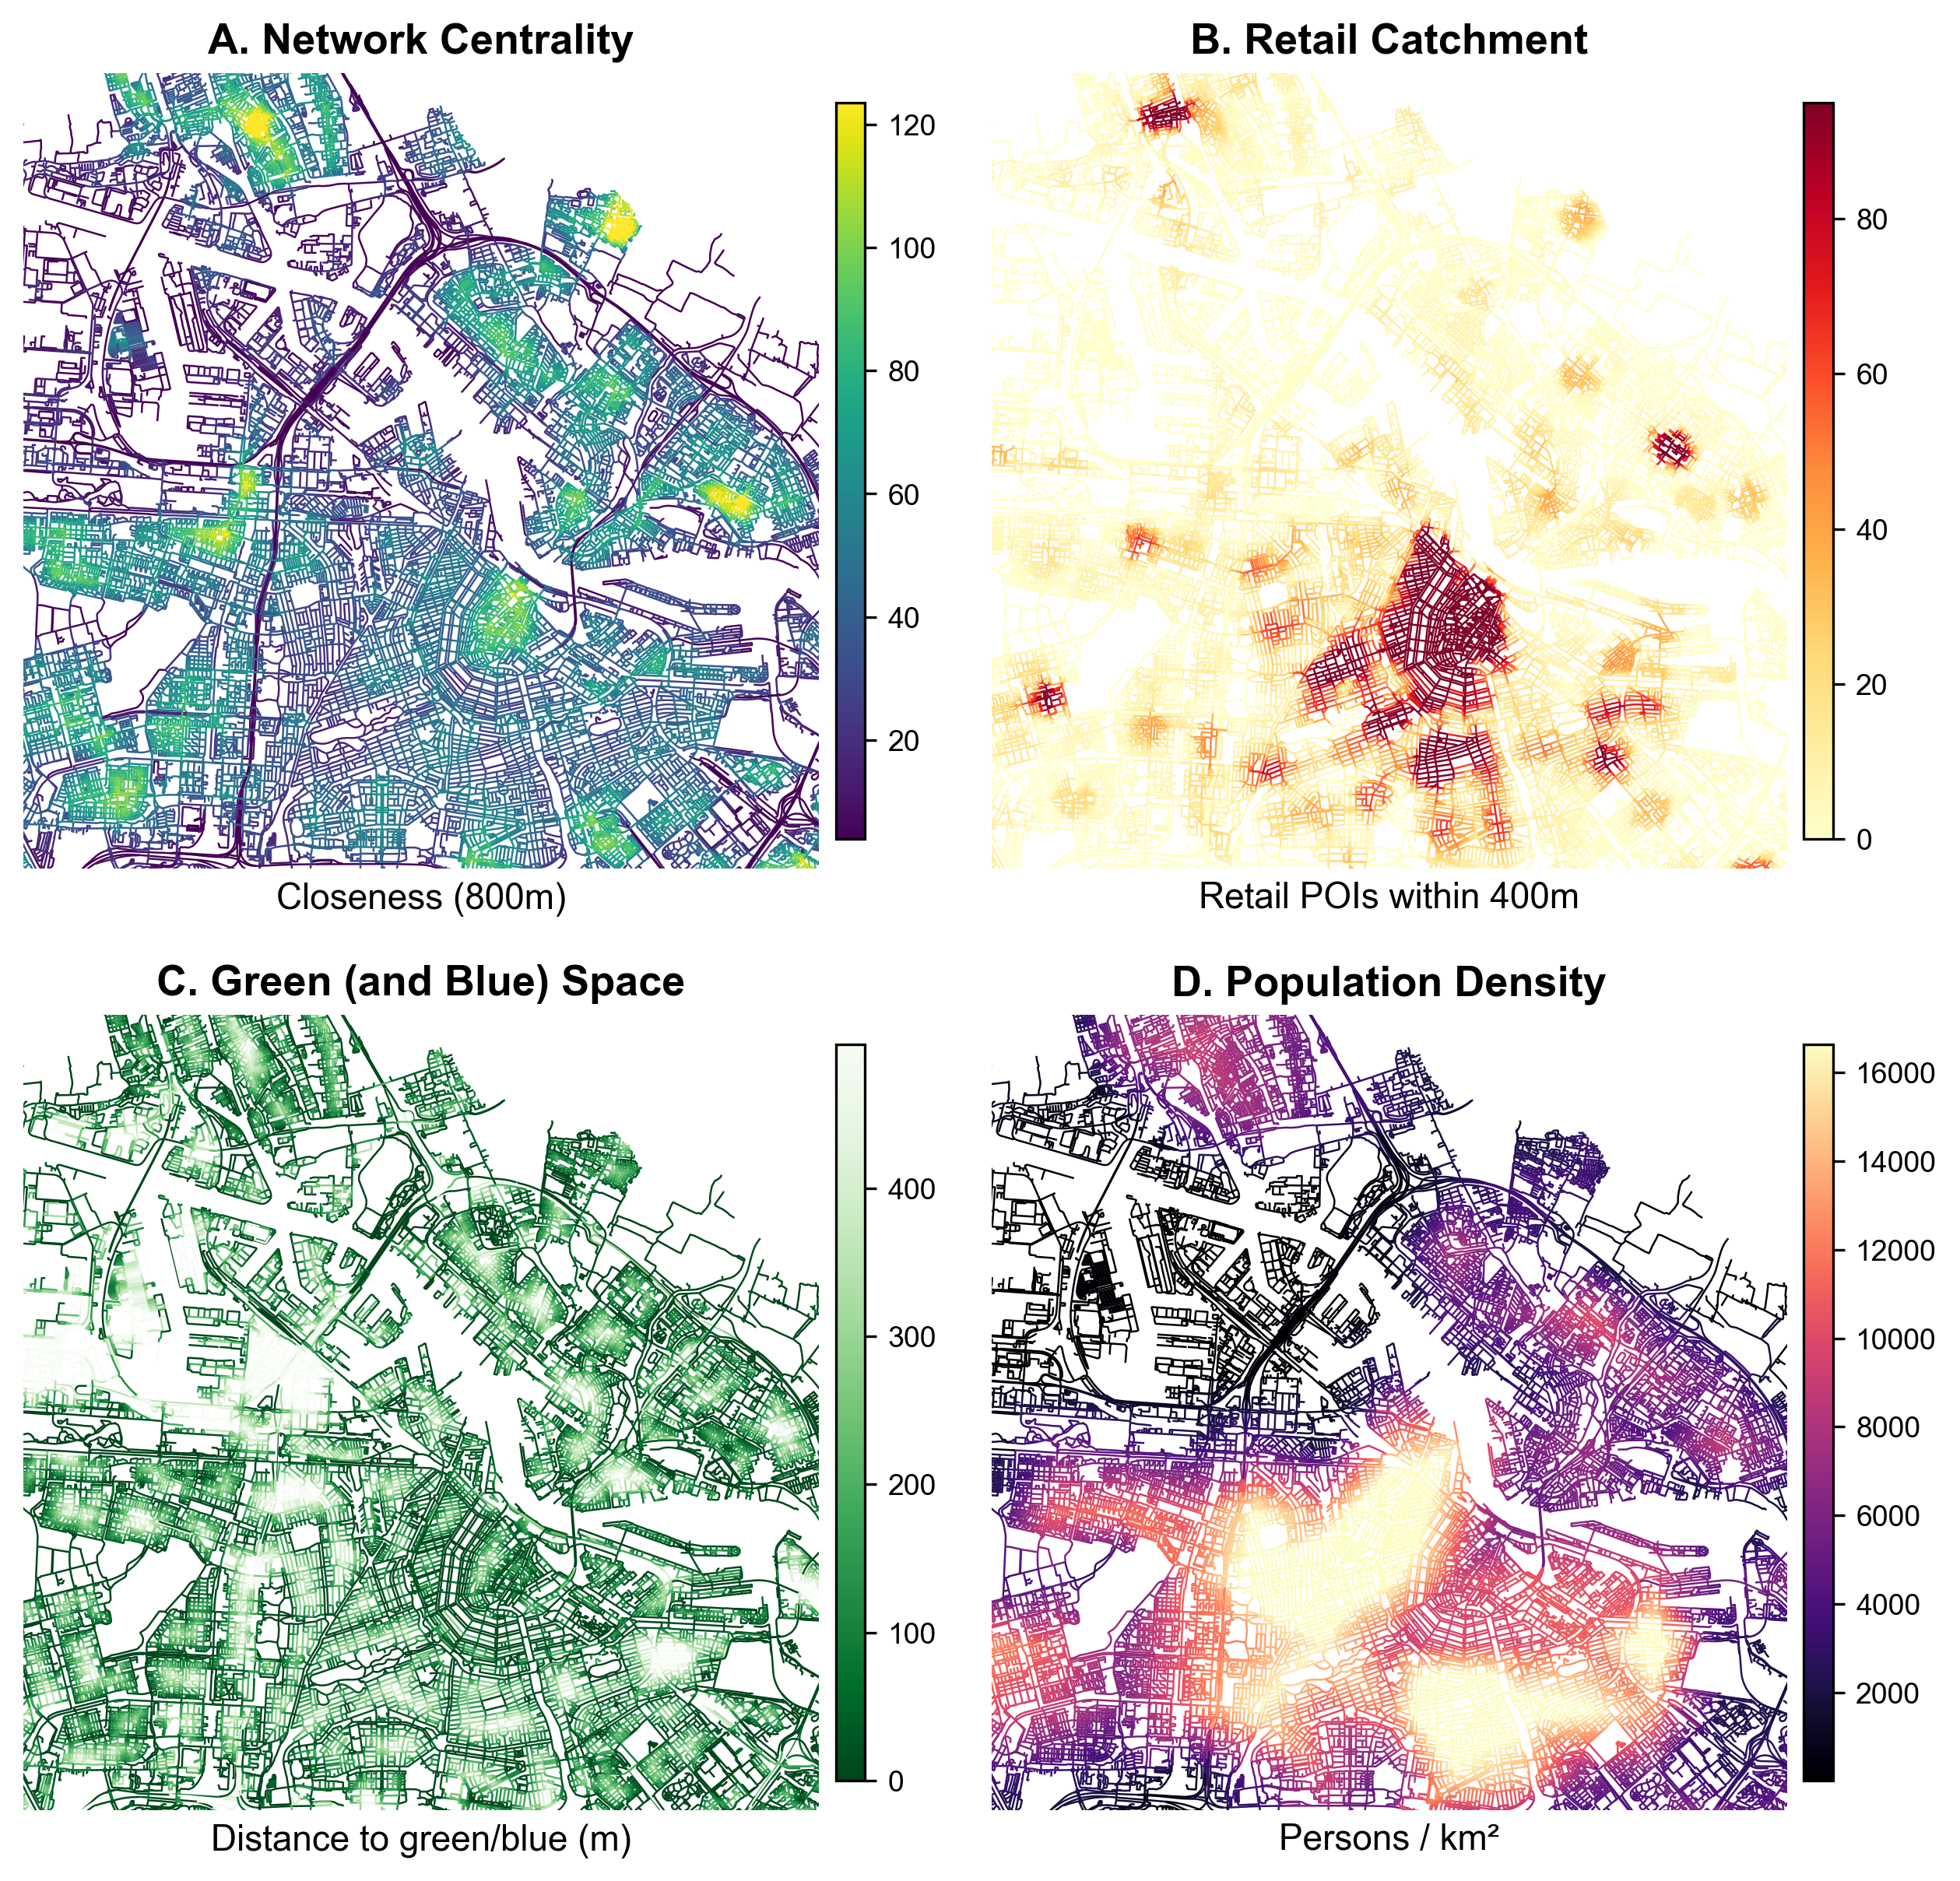
\includegraphics[width=\textwidth]{outputs/figures/fig_example_amsterdam.png}
  \caption{\textbf{Example SOAR-EU output for Amsterdam, Netherlands.} Street segments coloured by computed metrics: (A) closeness centrality at 800\,m threshold; (B) retail catchment (POI count within 400\,m); (C) distance to nearest green or blue space; (D) population density (persons/km\textsuperscript{2}, Eurostat Census Grid 2021). Different spatial scales and metric types lend themselves to different forms of analysis.}
  \label{fig:example-amsterdam}
\end{figure}

%% ============================================================================
%% METHODS
%% ============================================================================
\section{Methods}

Sections~\ref{sec:study-area}--\ref{sec:implementation} describe the processing pipeline (Figure~\ref{fig:pipeline}); Section~\ref{sec:provenance} discusses data provenance and source quality; Section~\ref{sec:poi-pattern-characterisation} provides scale-dependent usage guidance for POI-derived metrics. All source datasets were ingested during mid 2026 using the release versions indicated in Table~\ref{tab:sources}; the final dataset snapshot used for validation and distribution corresponds to Zenodo deposit \ZenodoDoi{}.

\begin{figure}[htbp]
  \centering
  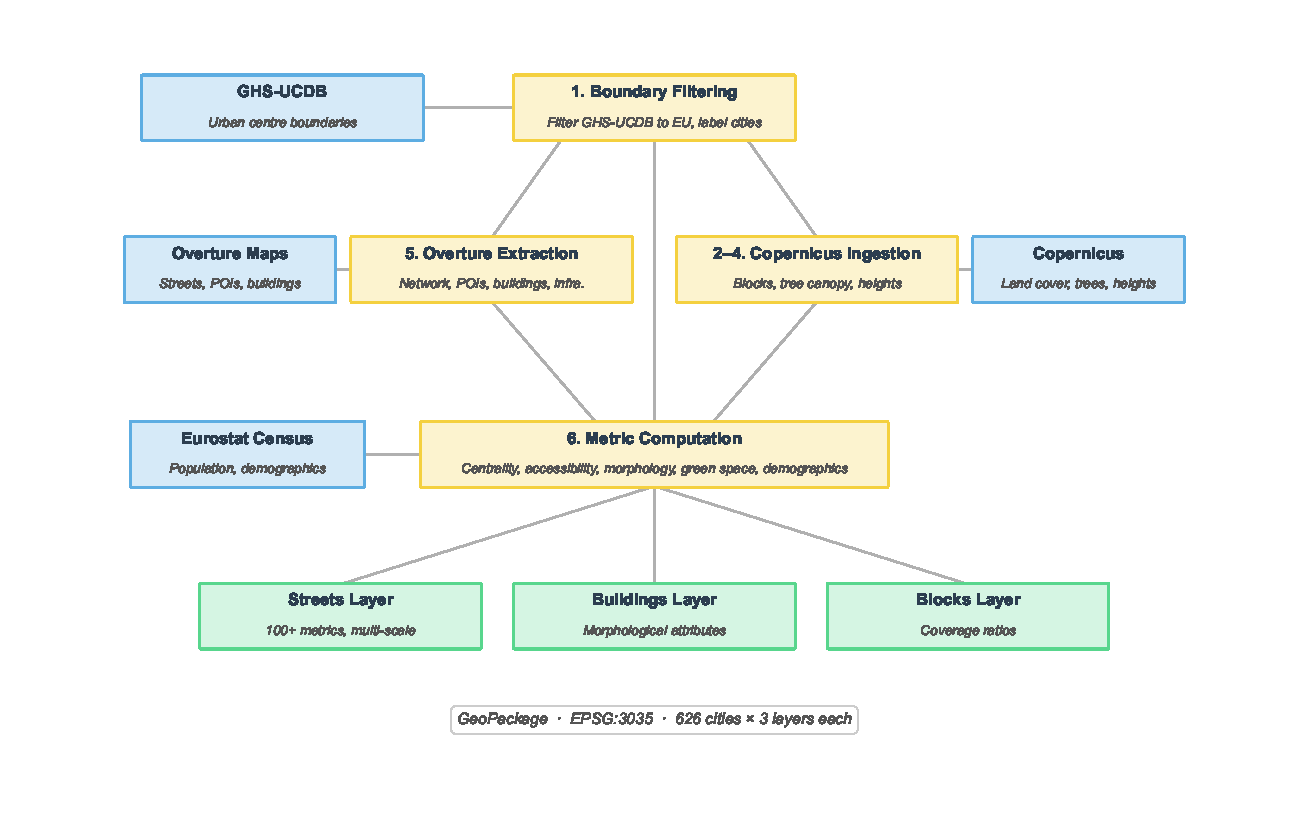
\includegraphics[width=0.85\textwidth]{outputs/figures/fig_pipeline.pdf}
  \caption{\textbf{SOAR-EU processing pipeline.} Four open data sources (blue) feed four processing stages (yellow) that produce three GeoPackage output layers per city (green). Stage~1 filters GHS-UCDB boundaries to the EU and labels cities; Stages~2--5 ingest Copernicus and Overture data in parallel; Stage~6 computes all metrics using the ingested layers, Eurostat census data, and the filtered boundaries.}
  \label{fig:pipeline}
\end{figure}

\subsection{Study Area Definition}
\label{sec:study-area}

Urban boundaries derive from the Global Human Settlement Layer Urban Centre Database (GHS-UCDB) R2024A \cite{ghsl2024}, which defines urban centres using the Degree of Urbanisation (DEGURBA) methodology: contiguous 1$\times$1~km grid cells with $\geq$1,500 inhabitants/km\textsuperscript{2} (or $\geq$50\% built-up surface) and cumulative population $\geq$50,000. Filtering to continental Europe (EPSG:3035) yielded \NCitiesTotal{} urban centres. All meet the $\geq$50,000 population threshold and thus correspond to cities or major urban agglomerations rather than small towns. City names are taken directly from the GHS-UCDB \texttt{GC\_UCN\_MAI\_2025} (Main Urban Centre Name) attribute. Because GHS-UCDB boundaries reflect population density contours rather than administrative units, assigned names may not always correspond to commonly used city names (e.g., a district name rather than the parent municipality).

\subsection{Data Sources}

Table~\ref{tab:sources} summarises input datasets.

Street networks from Overture Maps \cite{overture2026} were cleaned via cityseer \cite{simons2023}, following the automated network-cleaning procedure described in \cite{abdeldayem2026}: disconnected components were removed and degree-2 nodes collapsed. Level-aware processing prevents incorrect merging at bridges or tunnels. The 8\,m cleaning tolerance is deliberately conservative, prioritising consistent processing across all cities over city-specific fine-tuning.

POI categories from Overture's ``places'' theme were mapped to 11 analytical classes (Table~\ref{tab:landuse}; derivation in Section~\ref{sec:landuse-access}), and infrastructure points from Overture's infrastructure theme to three categories (transport, parking, street furniture; Table~\ref{tab:infrastructure}). Land cover and tree canopy derive from Copernicus Urban Atlas \cite{eea2021ua} and Street Tree Layer \cite{eea2021stl} respectively. Building heights were sampled from the Digital Height Model \cite{eea2012bh}.

Demographics from Eurostat Census Grid 2021 \cite{eurostat2024} include population, employment, age structure, nationality, and migration at 1~km\textsuperscript{2} resolution.

\begin{table}[H]
  \centering
  \caption{Input data sources and their roles in the processing pipeline.}
  \label{tab:sources}
  \small
  \begin{tabular}{@{}L{2.5cm}L{1.6cm}L{1cm}L{2.8cm}L{3.2cm}@{}}
    \toprule
    \textbf{Dataset} & \textbf{Source} & \textbf{Year} & \textbf{Licence} & \textbf{Use} \\
    \midrule
    GHS-UCDB R2024A & JRC/GHSL & 2024 & \href{https://commission.europa.eu/legal-notice_en\#copyright-notice}{EC reuse policy} & Urban boundaries \\
    Street networks & Overture Maps & 2026 & \href{https://opendatacommons.org/licenses/odbl/1-0/}{ODbL} & Centrality, accessibility \\
    Points of interest & Overture Maps & 2026 & \href{https://cdla.dev/permissive-2-0/}{CDLA-Permissive-2.0} & Land-use metrics \\
    Building footprints & Overture Maps & 2026 & \href{https://opendatacommons.org/licenses/odbl/1-0/}{ODbL} & Morphology \\
    Urban Atlas & Copernicus & 2021 & \href{https://land.copernicus.eu/en/data-policy}{Copernicus data policy} & Blocks, green space \\
    Street Tree Layer & Copernicus & 2021 & \href{https://land.copernicus.eu/en/data-policy}{Copernicus data policy} & Tree proximity \\
    Height Model & Copernicus & 2012 & \href{https://land.copernicus.eu/en/data-policy}{Copernicus data policy} & Building heights \\
    Census Grid & Eurostat & 2021 & \href{https://commission.europa.eu/legal-notice_en\#copyright-notice}{EC reuse policy} & Demographics \\
    \bottomrule
  \end{tabular}
\end{table}

\subsection{Data Processing Pipeline}

The pipeline comprises six stages executed via Python modules (Table~\ref{tab:pipeline}). All scripts support idempotent execution (existing outputs are skipped unless \texttt{overwrite} is specified), enabling incremental processing and failure recovery.

\begin{table}[H]
  \centering
  \caption{Processing pipeline stages with corresponding Python modules.}
  \label{tab:pipeline}
  \small
  \begin{tabular}{@{}cL{6cm}L{6cm}@{}}
    \toprule
    \textbf{Stage} & \textbf{Module} & \textbf{Description} \\
    \midrule
    1 & \texttt{src.data.generate\_boundary\_polys} & Filter GHS-UCDB boundaries to continental Europe \\
    2 & \texttt{src.data.load\_urban\_atlas\_blocks} & Extract Urban Atlas blocks per boundary \\
    3 & \texttt{src.data.load\_urban\_atlas\_trees} & Extract Street Tree Layer per boundary \\
    4 & \texttt{src.data.load\_bldg\_hts\_raster} & Clip building height rasters per boundary \\
    5 & \texttt{src.data.load\_overture} & Extract Overture data (network, POIs, buildings, infrastructure) \\
    6 & \texttt{src.processing.generate\_metrics} & Compute all metrics per boundary \\
    \bottomrule
  \end{tabular}
\end{table}

For accurate metric computation at boundary edges, input datasets are buffered beyond city boundaries. Street networks are buffered by 10\,km, giving nodes near boundaries a complete network context for centrality calculations. Points of interest, buildings, and infrastructure are buffered by 2\,km, capturing all reachable amenities for boundary-proximate locations. Copernicus land cover and tree canopy data is clipped to boundary bounding boxes for green-space proximity coverage.

\subsection{Metric Computation}
\label{sec:metric-computation}

\subsubsection{Network Centrality}
Network centrality metrics quantify a location's connectivity within the street network and were computed using the cityseer package \cite{simons2023}.

Closeness variants measure how accessible a location is relative to the rest of the network: beta-weighted closeness (gravity index with exponential distance decay), harmonic closeness (sum of inverse distances), Hillier-type closeness (node count divided by average node distance), farness (sum of distances), and street segment density. The density measure (\texttt{cc\_density\_DDD}) is an unweighted count of network nodes, each corresponding to a natural street-segment midpoint after cleaning, reachable within the network-distance threshold; it is not weighted by segment lengths. Betweenness centrality measures how often a location lies on shortest paths between other locations and is computed in both standard and distance-weighted forms.

Metrics were generated using cityseer's shortest-path centrality (\texttt{centrality\_shortest}) at thresholds of 400\,m, 800\,m, 1,200\,m, 1,600\,m, 4,800\,m, and 9,600\,m, corresponding to 5--120 minute walking catchments at 80\,m/min average pedestrian speed. These thresholds span local-to-global catchments: 400\,m captures immediate neighbourhood context; 800\,m reflects typical distances walked to transit; the 1,200--1,600\,m range corresponds to 15-minute walking catchments; 4,800\,m characterises district-scale network structure; and 9,600\,m extends to city-wide connectivity. Centralities are measured using shortest paths (as opposed to angular paths) for greater tolerance of artefacts deriving from automated street cleaning procedures.

\subsubsection{Land-Use and Infrastructure Accessibility}
\label{sec:landuse-access}
Points of interest from Overture Maps were classified into the 11 aggregated land-use categories distributed with the dataset (Table~\ref{tab:landuse}). The aggregation follows Overture's own top-level groupings to the extent possible, rather than imposing a re-engineered taxonomy: most of the 11 categories correspond directly to a single Overture top-level class, with only two consolidations (\texttt{eat\_and\_drink} merging restaurants, bars, and cafés; \texttt{business\_and\_services} merging eleven Overture professional and commercial sub-classes) and two renames (\texttt{public\_services} from \texttt{public\_service\_and\_government}, \texttt{religious} from \texttt{religious\_organization}). The complete mapping from Overture's 2,000+ leaf categories to analytical classes is detailed in Supplementary Material (Section~S2).

Overture's separate infrastructure theme is grouped into three further accessibility categories (transport, parking, and street furniture; Table~\ref{tab:infrastructure}), which receive the identical network-accessibility treatment described below.

Accessibility metrics aggregate POI counts over the street network at the same street-segment locations used for centrality computations, enabling direct comparison between network structure and land-use distribution \cite{simons2023}. Network-based distances are used throughout, rather than Euclidean buffers or zonal aggregation.

For each land-use and infrastructure category, both unweighted counts (reachable POIs within $d_{\max}$) and distance-weighted counts (applying exponential decay $e^{-\beta d}$, where $\beta = 4/d_{\max}$ such that weight falls to approximately 0.018 at the distance threshold) were computed, alongside nearest-distance measures. Distance-weighted counts reflect how amenity usage decays with distance (a caf\'{e} at 100\,m contributes more than one at 1,000\,m), while unweighted counts offer simpler interpretability.

The exponential weight never reaches zero, so an establishment infinitely far would still make an infinitesimal contribution. To keep each measure finite and tied to a walkable catchment, a threshold distance $d_{\max}$ is imposed rather than integrating over the entire network. The decay rate is set at $\beta = 4/d_{\max}$ where the weight has already fallen to under 2\% by the time it reaches $d_{\max}$, thereby discarding the infinitely long tail with minimal impact on the aggregations. The threshold distances are chosen for rounding convenience and the provision of a range of thresholds lets users choose the catchment that suits the intended usage scenario.

Mixed-use diversity was quantified using Hill numbers \cite{hill1973}. Hill numbers at $q=0$ equal richness (count of distinct land-use types); at $q=1$, the exponential of Shannon entropy; at $q=2$, the inverse Simpson index. We compute all three variants in both unweighted and distance-weighted forms, where the distance-weighted forms follow the same weighting conventions as described for land-use accessibility.

\subsubsection{Morphology}
Building and block morphology metrics were computed using the momepy package \cite{fleischmann2019}, which provides standardised urban morphometric functions.

For each building footprint, we compute: area, perimeter, circular compactness, orientation, corners count, shape index, fractal dimension, and shared wall ratio (fraction of perimeter shared with adjacent buildings). Building heights are extracted from the Copernicus Height Model raster by buffering each footprint by 10\,m (one DHM pixel) and averaging valid (non-null) overlapping pixel values. The single-pixel buffer ensures that small footprints (those contained within a single pixel) and footprints with minor misregistration against the 2012 raster still receive a height sample; the trade-off is some smoothing in dense fabric where party-wall neighbours and narrow courtyards fall within the buffer. The height value enables computation of volume and form factor. Floor area (assuming 3\,m floor height) is computed per building as an intermediate for block-level FSI but is not retained as a standalone aggregated metric.

Block morphology uses only built-up Urban Atlas blocks: 14 non-built land-cover classes (green areas, forests, agriculture, water, wetlands, and sports/leisure facilities) are excluded before morphometric computation and aggregation of the metrics to the adjacent streets. For the remaining blocks, we compute geometric properties (area, perimeter, circular compactness, orientation) and Spacematrix indicators \cite{haupt2010}: ground space index (GSI, building footprint area divided by block area), floor space index (FSI, total floor area divided by block area), open space ratio (OSR $= (1 - \text{GSI}) / \text{FSI}$), mean number of storeys (L $= \text{FSI} / \text{GSI}$), and area-weighted mean building height. Blocks exceeding 2\,km\textsuperscript{2} are additionally excluded as oversized infrastructural or transitional polygons (the threshold separates typical urban blocks from large airport, port, industrial, or transitional polygons that occur in the Urban Atlas layer); blocks below 1\% building coverage receive NaN for all Spacematrix metrics, since the ratios become numerically unstable as their denominators (GSI, FSI) approach zero.

Building and block metrics are aggregated to streets via nearest-network-distance assignment within 200\,m and 400\,m thresholds. Each building or block centroid is assigned to the nearest street, and statistics (median and median absolute deviation) are computed across all features within each threshold distance. For building area and volume, sum statistics are additionally retained; for block area, only the sum is additionally retained. Building height is also aggregated (as median and MAD of individual building heights per street).

In addition, a bilateral street-frontage ratio is computed per street segment as a source-robust measure of building continuity. For each street, a 35\,m buffer defines a corridor; all building edges whose midpoint falls inside the corridor and whose nearest street is this one are identified. Per side (left/right of the centreline), only edges within 5\,m of the closest edge are retained, filtering out rear extensions and garages while preserving the primary facade line. The score is the fraction of street length covered by the retained edges on the more-covered side (3\,m trimmed from each end as a junction guard). Unlike shared wall ratio, which requires exact topological contact between adjacent polygon boundaries, frontage ratio depends only on building \emph{presence} along the street edge. It is therefore insensitive to unintended gaps and to the lack of delineation between neighbouring buildings that is characteristic of ML-derived footprints, where segmentation pipelines lack the cadastral subdivision information available to community-contributed sources (see Section~\ref{sec:provenance}).

\subsubsection{Green Space Proximity}
Network distance to nearest green space polygon edge was computed for each street. Green spaces derive from 12 Urban Atlas land cover classes: public and unknown-access urban green areas, forests, herbaceous vegetation, open spaces with little or no vegetation, wetlands, water bodies, pastures, arable land, permanent crops, mixed cultivation, and orchards (full list in Supplementary Material Section~S3). Sports and leisure facility blocks often function as green space (e.g., open playing fields) but can also be heavily built up (e.g., stadiums, indoor arenas); we therefore apply a consistent 20\% building-coverage threshold, including the block as green space when built coverage is below 20\% and excluding it otherwise.

Polygon boundaries are sampled at 20\,m intervals to generate point features for distance calculations, improving accuracy for large or irregularly-shaped polygons. For each street, only the distance to the single nearest sampled point is retained, so a polygon contributes to a given street at most once regardless of how many of its boundary samples lie within range. Tree canopy proximity uses Street Tree Layer polygons with equivalent sampling. Green space and tree canopy areas are also aggregated within walking distances (200\,m, 400\,m, 800\,m) to quantify local coverage.

\subsubsection{Demographic Interpolation}
Census grid values were interpolated to street-segment midpoints using Delaunay-based linear barycentric interpolation (\texttt{scipy.interpolate.griddata}, method \texttt{linear}) from 1\,km grid cell centroids. Interpolated variables include: total population (\texttt{t}), population density (\texttt{density}), male/female counts (\texttt{m}, \texttt{f}), age cohorts (\texttt{y\_lt15}, \texttt{y\_1564}, \texttt{y\_ge65}), employment (\texttt{emp}), nationality (\texttt{nat}, \texttt{eu\_oth}, \texttt{oth}), and migration flows (\texttt{same}, \texttt{chg\_in}, \texttt{chg\_out}). Percentage variants (suffixed with \texttt{\_\%}) are computed for each variable relative to total population. Linear interpolation from 1\,km\textsuperscript{2} source cells produces smooth gradients that do not represent sharp sub-cell discontinuities (industrial estates, large parks, transit corridors); these street-level demographic values should be read as neighbourhood-scale context rather than as fine-grained block-level estimates.

\subsection{Implementation}
\label{sec:implementation}

The pipeline is implemented in Python 3.12 with modules for data ingestion, metric processing, utilities, and land-use classification. Network loading retrieves Overture ``connector'' and ``segment'' themes via STAC, transforms to EPSG:3035, and applies cityseer cleaning (8\,m tolerance, 100-node minimum component size). POI loading maps Overture's 2,000+ raw categories to 23 intermediate classes via a CSV lookup (preserved in the code repository for transparency and reuse), which are then aggregated to the 11 analytical categories distributed with the dataset (Table~\ref{tab:landuse}).

Table~\ref{tab:parameters} summarises the fixed processing parameters ensuring reproducibility across all urban centres.

\begin{table}[!htbp]
  \centering
  \caption{Fixed processing parameters for reproducibility.}
  \label{tab:parameters}
  \small
  \begin{tabular}{@{}L{4cm}L{3cm}L{4.5cm}@{}}
    \toprule
    \textbf{Parameter} & \textbf{Value(s)} & \textbf{Rationale} \\
    \midrule
    Network cleaning tolerance & 8\,m & Consolidate near-parallel edges \\
    Min.\ component size & 100 nodes & Remove disconnected fragments \\
    Centrality thresholds & 400, 800, 1200, 1600, 4800, 9600\,m & 5--120 minute walking catchments \\
    Accessibility thresholds & 200, 400, 800, 1200, 1600\,m & Pedestrian-scale proximity \\
    Morphology aggregation & 200, 400\,m & Immediate building context \\
    Green space proximity & 1600\,m & Extended walkable distance \\
    Green area aggregation & 200, 400, 800\,m & Multi-scale green coverage \\
    \bottomrule
  \end{tabular}
\end{table}

Outputs are written as GeoPackage files in EPSG:3035 following the structure described in Section~\ref{sec:dataset-structure}. Dependencies are pinned via \texttt{pyproject.toml}; core packages include cityseer, momepy, geopandas, and overturemaps.

\subsection{Data Provenance}
\label{sec:provenance}

SOAR-EU integrates data layers with different provenance. Eurostat boundaries, census data, and Copernicus land cover follow documented methodologies with full pan-European coverage. Street networks derive from OpenStreetMap via Overture, whose road coverage is largely complete across urbanised Europe \cite{barringtonleigh2017}.

Building footprints derive from Overture Maps, which conflates multiple sources in a fixed priority order: community-contributed datasets (OpenStreetMap, Esri Community Maps, national cadastres) take precedence over ML-derived datasets (Microsoft ML Building Footprints, Google Open Buildings). When two sources contain the same building (IoU~$\geq$~50\%), the higher-priority source's geometry is retained; ML-derived footprints fill areas not covered by community sources. Each footprint carries a \texttt{sources} attribute recording which dataset contributed it, enabling downstream filtering by provenance.

In European cities, OpenStreetMap is typically the dominant contributor. Herfort et al.\ \cite{herfort2023} analysed OSM building completeness across 13{,}189 urban agglomerations worldwide and found Europe and Central Asia to have the highest regional average (71\%), though within-region coverage remains uneven. Countries with completed cadastral imports---France (DGFiP cadastre), the Netherlands (BAG), and Belgium/Flanders (GRB)---are generally considered to have a high degree of community-sourced building coverage. In contrast, several southern and eastern European countries (including Romania, Bulgaria, Greece, Hungary, and Portugal) lack such imports and, in our data, rely more heavily on Microsoft's ML-derived footprints. Such ML-derived footprints overlap imperfectly with reference building data \cite{minghini2024}, as they are segmented from imagery rather than digitised from cadastre. Across the \NCitiesTotal{} cities in SOAR-EU, the proportion of ML-derived footprints ranges from near-zero in countries with complete cadastral imports to substantial in several southern and eastern European countries; per-city and per-country breakdowns are provided in the accompanying \texttt{building\_source\_counts.csv} and \texttt{building\_source\_by\_country.csv} (summarised in Supplementary~\S\ref{sec:bldg-supp}), and per-city completeness can be cross-referenced against the ohsome OSM-completeness map at \url{https://hex.ohsome.org/#/urban_building_completeness}.

ML-derived footprints expand coverage but introduce quality trade-offs relevant to morphometric computation. Because they are segmented from overhead imagery rather than digitised from cadastral plans, they delineate roof outlines rather than ground-level footprints and can merge adjacent structures into single polygons or leave gaps that break the topological adjacency these metrics rely on. The effect is visible directly in our data: metrics that depend on exact polygon boundary coincidence (particularly shared wall ratio and, to a lesser extent, fractal dimension) are systematically affected, with shared wall ratio showing the strongest negative association between a city's ML fraction and its median value (full coefficients in Supplementary Table~\ref{tab:building_metric_sensitivity}; the within-city test in Supplementary~\S\ref{sec:bldg-supp} confirms this as a per-building artefact rather than a country-level morphological gradient). Metrics based on polygon area and shape (compactness, orientation, shape index) show no significant association with source composition.

POI data derives primarily from commercial and editorial sources (e.g., Meta, Microsoft, Foursquare, OSM) via Overture, with variable coverage relative to official registries; this is characterised in detail in Section~\ref{sec:poi-pattern-characterisation}. Temporal currency and other cross-layer caveats are summarised under Limitations of the Dataset.

\subsection{POI-derived accessibility: source-substitution analysis}
\label{sec:poi-pattern-characterisation}

Because Overture's POI layer aggregates commercial and crowdsourced data of varying completeness, the reliability of derived metrics varies across categories and spatial scales. To characterise where agreement holds and where it does not, we recompute POI-derived outputs against independent official registries in the two countries for which suitable national registries are openly available: France (SIRENE, \NRefCitiesFr{} cities) and the Netherlands (BAG, \NRefCitiesNl{} cities), \NRefCities{} reference cities in total. This validation therefore speaks directly to French and Dutch coverage; cities elsewhere in Europe (particularly in southern and eastern Europe, where OpenStreetMap-derived coverage is less mature) are outside its scope and should be treated with the additional caution discussed under Limitations of the Dataset. We frame the comparison around three questions that capture the main analytical uses of the resulting metrics:
\begin{itemize}
  \item \textbf{How many, relative to elsewhere?} Whether locations are ranked consistently by how much of a particular land use they can access. This is a pattern-agreement question as opposed to one of absolute counts: Overture is known to undercount relative to official registries (further discussed below), so the analytically useful question is whether that undercounting preserves the spatial ordering of accessibility.
  \item \textbf{Where are the hotspots?} Which locations fall in the top tier of activity.
  \item \textbf{How far is the nearest?} Whether the land use is reachable within a given distance threshold.
\end{itemize}
For each question, we measure agreement between Overture- and registry-derived accessibility for every street segment, then summarise within cities and across cities for each category and spatial scale (Figure~\ref{fig:pointa_support_heatmap}; Table~\ref{tab:pointa_minima}).

\subsubsection{Source-substitution replication}

\begin{figure}[!htb]
  \centering
  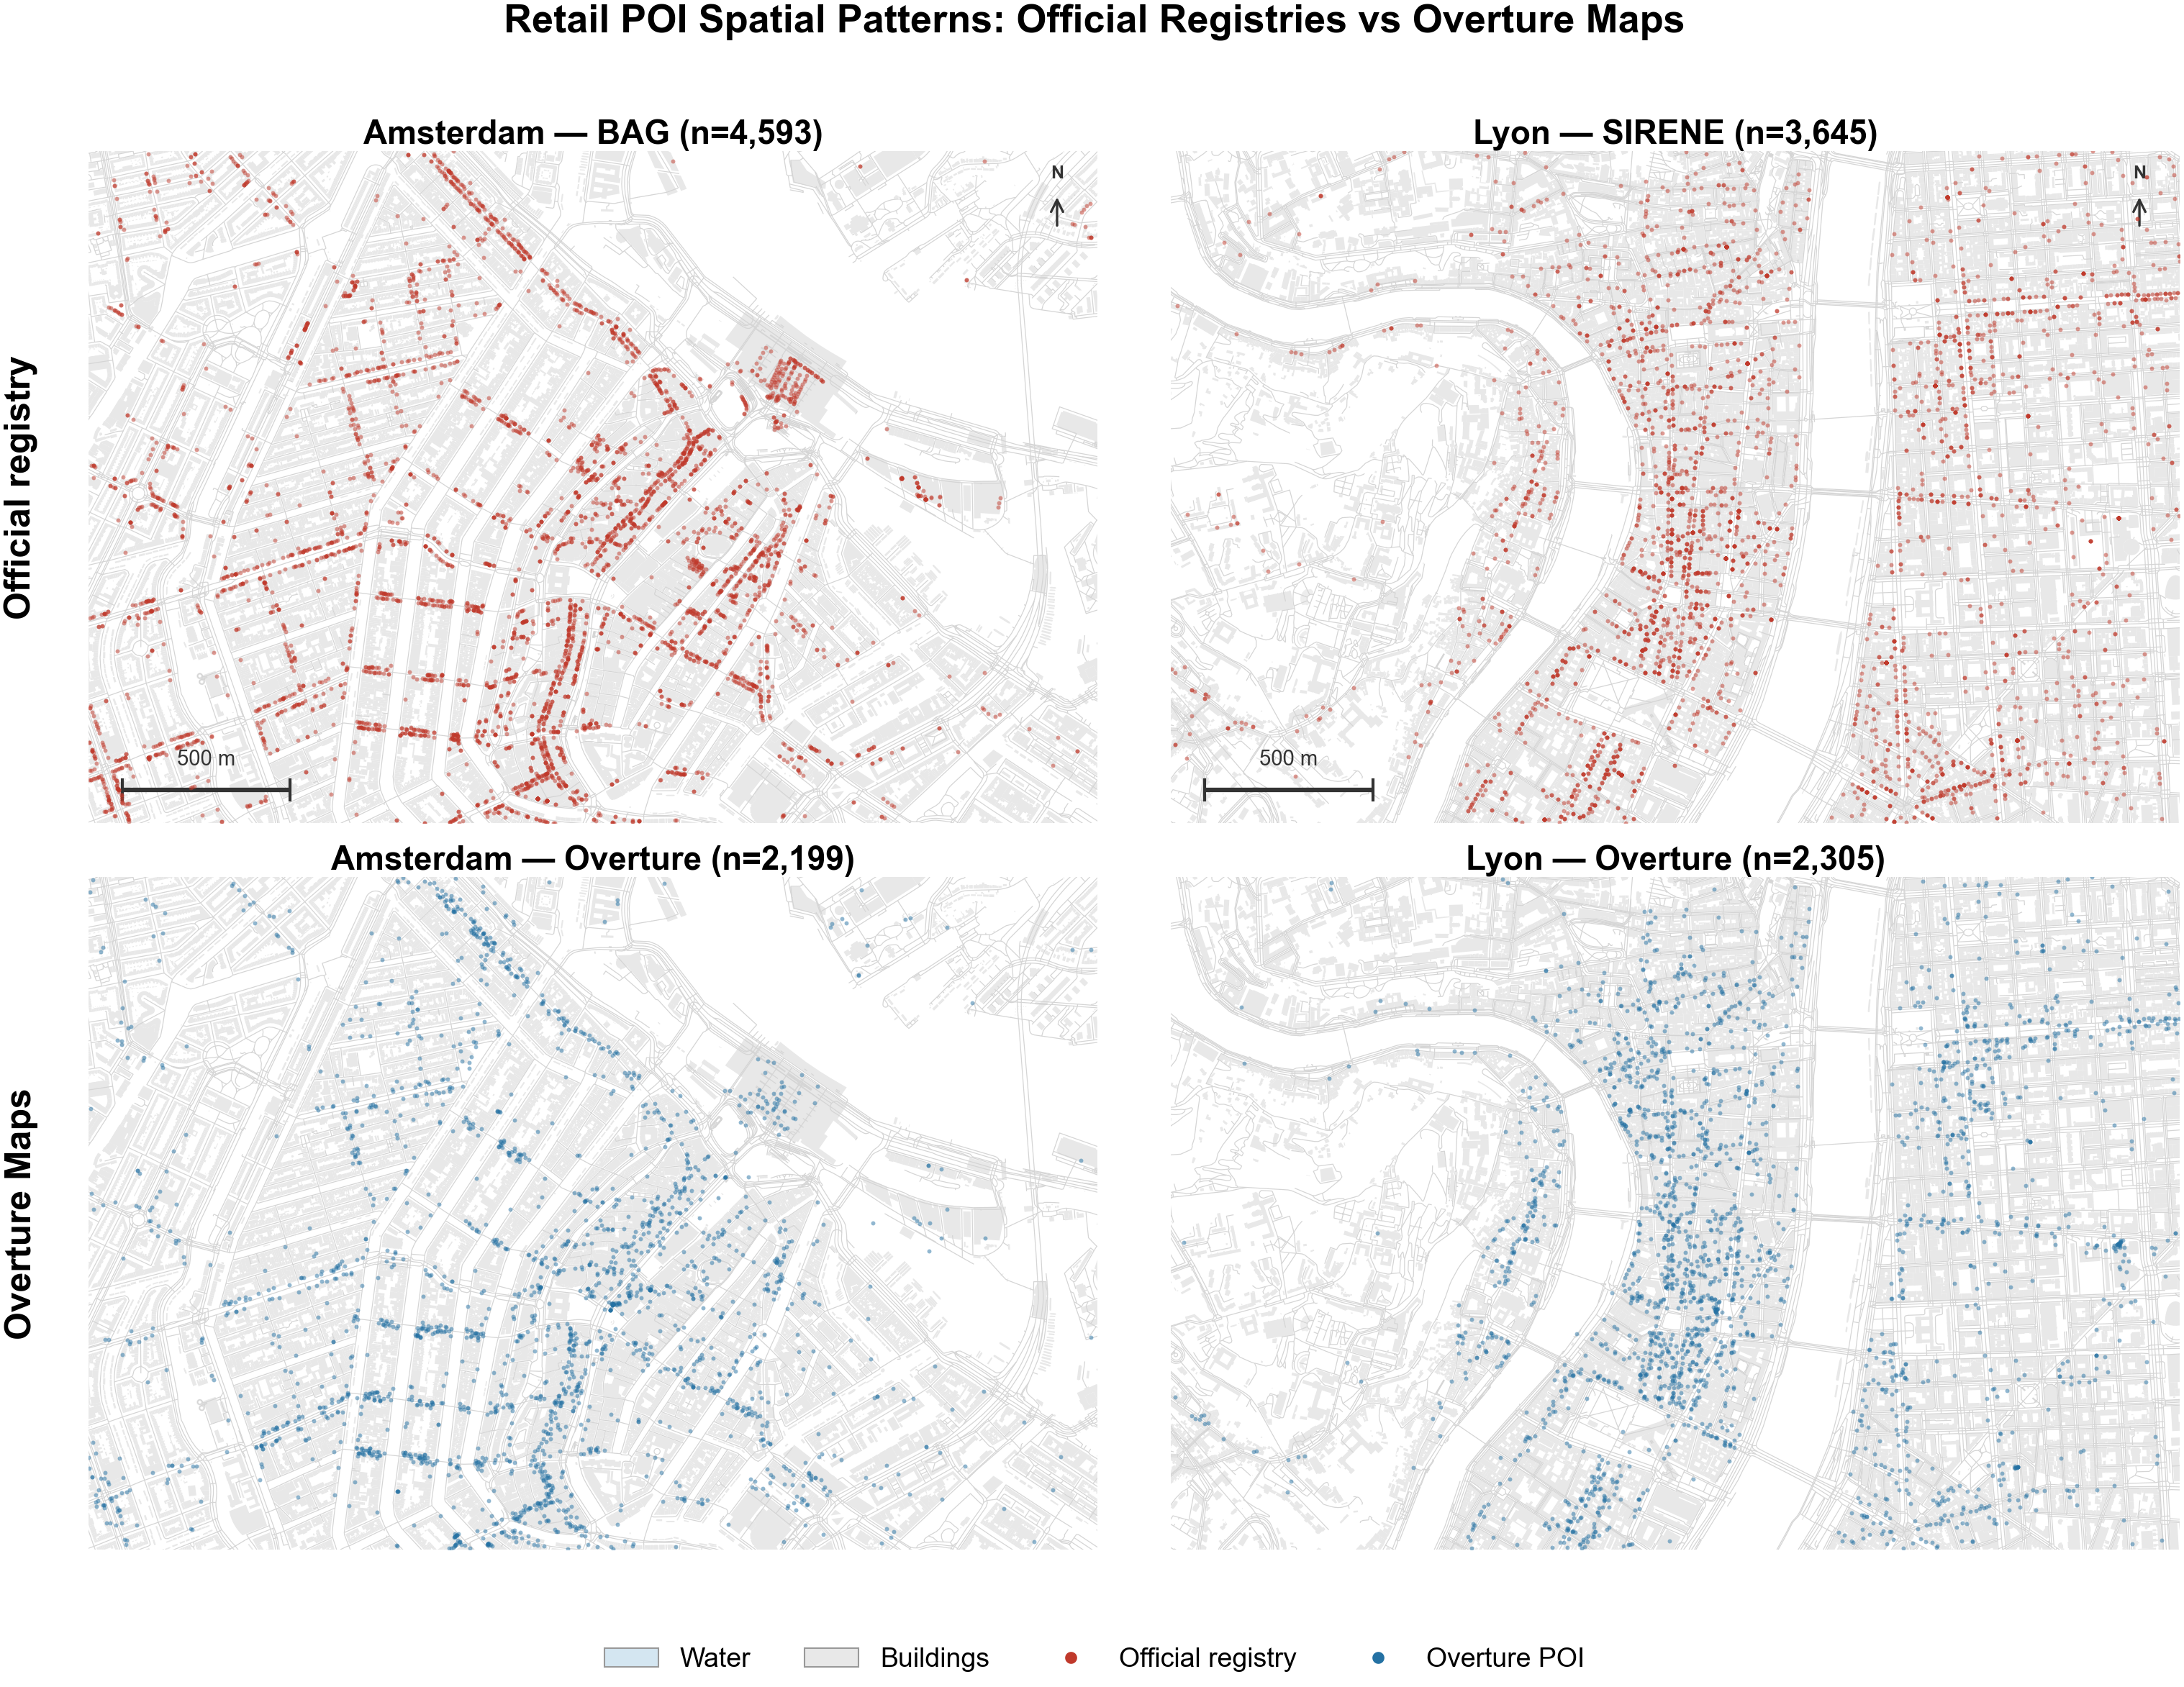
\includegraphics[width=\textwidth]{outputs/figures/fig_poi_spatial_comparison.png}
  \caption{\textbf{Retail POI locations from official registries (top) and Overture Maps (bottom)} for inner-city areas of Amsterdam (BAG; left) and Lyon (SIRENE; right). Point counts differ substantially between sources (Overture undercounts relative to the official registries), but the spatial clustering patterns are broadly consistent.}
  \label{fig:poi_spatial_comparison}
\end{figure}

\begin{figure}[p]
  \centering
  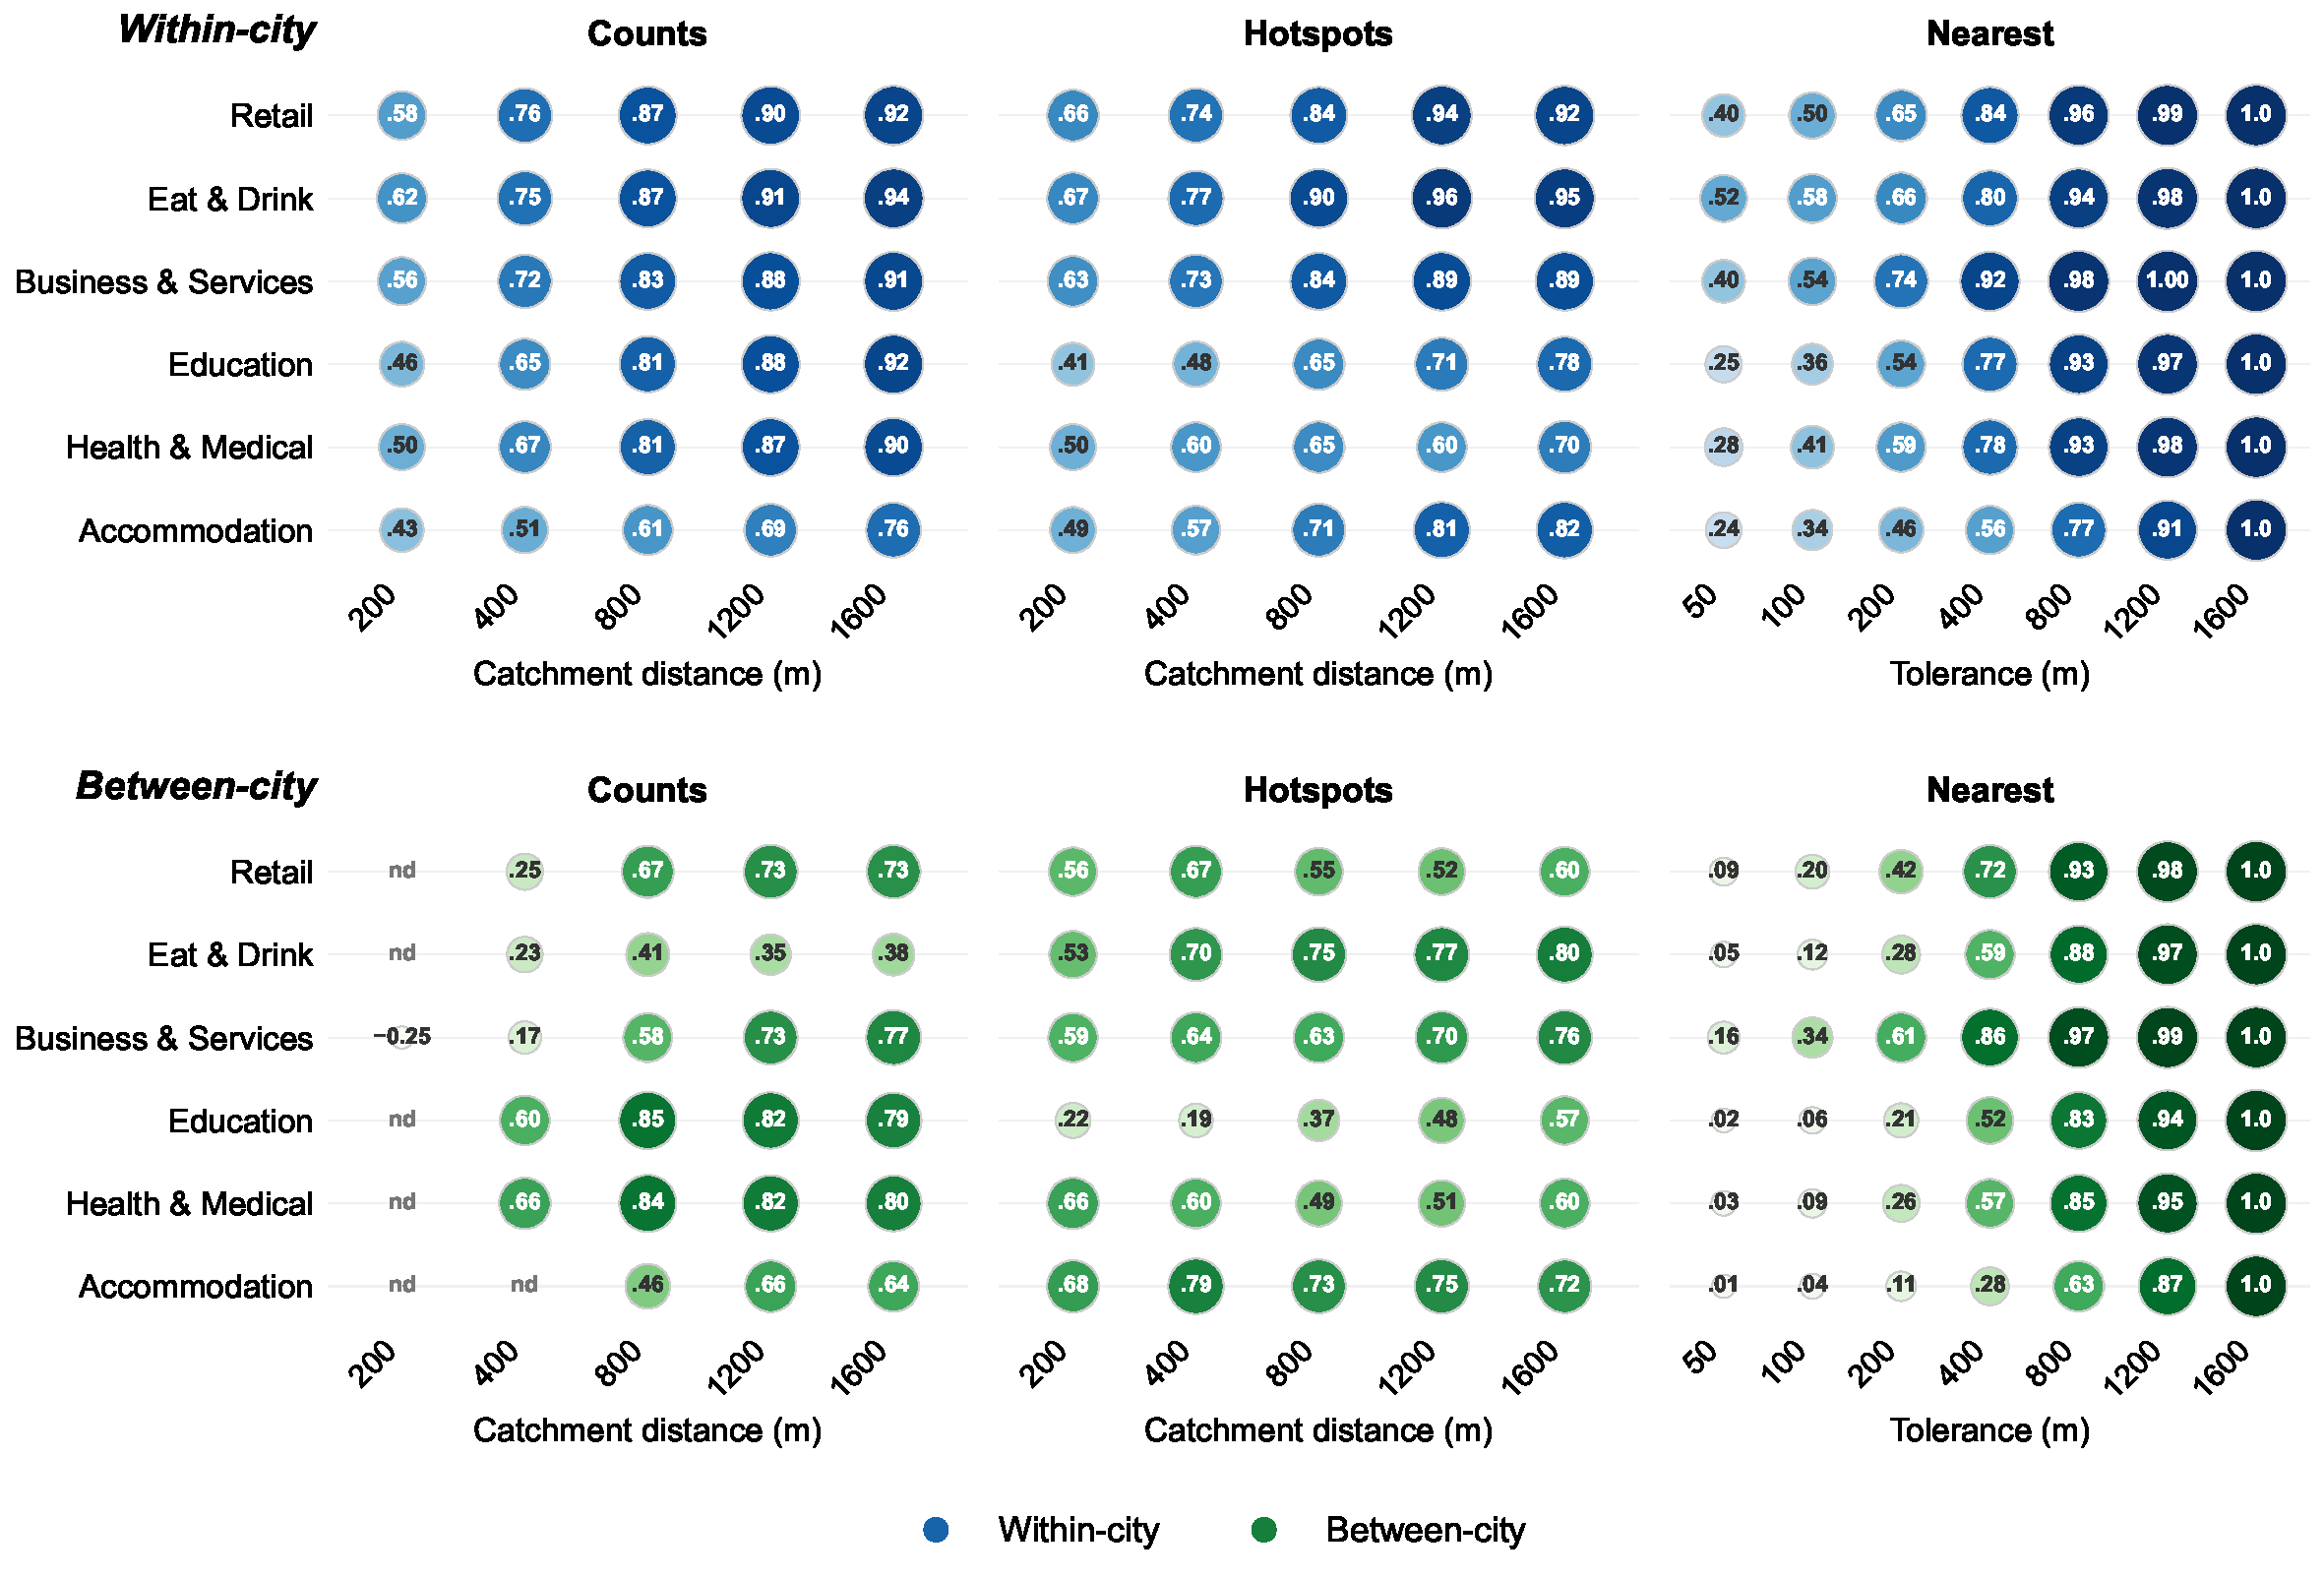
\includegraphics[width=\textwidth]{outputs/figures/fig_pointa_support_heatmap.pdf}
  \caption{\textbf{POI source-substitution agreement.}
    Agreement between Overture- and registry-based accessibility across all category--task--scale combinations. Top row (within-city): Spearman $\rho$ for segment-level rank correlation, top-10\% hotspot overlap, and nearest-distance F1. Bottom row (between-city): Spearman $\rho$ on city-level median counts and hotspot intensity, and harmonic-mean agreement of city-level nearest shares. Bubble size and annotation indicate the median score; colour distinguishes within-city from between-city scope. ``nd'' indicates insufficient data. Full agreement curves with bootstrap CIs appear in Supplementary Figure~\ref{fig:pointa_agreement_panels}.
  }
  \label{fig:pointa_support_heatmap}
\end{figure}

\begin{table}[p]
  \centering
  \caption{Minimum spatial scale (metres) at which each category's median agreement reaches $\geq$70\%, $\geq$75\%, $\geq$80\%, and $\geq$85\% concordance, grouped by scope (within-city, between-city) and metric family. For rank-correlation metrics, concordance is the fraction of observation pairs ranked identically by both sources, computed directly as $(1+\tau)/2$ where $\tau$ is the Kendall rank correlation (thresholds: $\tau \geq 0.40$, $0.50$, $0.60$, $0.70$). For overlap and F1 metrics the concordance fraction is used directly. Dashes indicate no tested scale reached that value.}
  \label{tab:pointa_minima}
  \scriptsize
  \input{outputs/tables/table_pointa_minima_clean}
\end{table}

We compute segment-level accessibility metrics twice for each reference city (\NRefCitiesFr{} in France via SIRENE \cite{sirene2026}; \NRefCitiesNl{} in the Netherlands via BAG \cite{bag2026}): once using Overture POIs and once using the official registry as input, holding the street network and all other inputs constant (see Figure~\ref{fig:poi_spatial_comparison} for an example). The question is not whether individual establishments match between sources, but whether the same network-based computations over different POI inputs produce consistent segment-level patterns of accessibility scores. Uncertainty is quantified at two levels: within-city spatial block bootstrap (distance-adaptive blocks, $B = 200$) captures segment-level spatial sampling variability, while a city-level bootstrap ($B = 2{,}000$) treats each city as an independent observation (see Supplementary~\S\ref{sec:poi-supp-bootstrap}). The reference set is concentrated in western Europe and country-specific results are in Supplementary~\S\ref{sec:poi-supp-city-variability}.

The two registries differ in granularity: SIRENE records individual business establishments with fine-grained activity codes that map relatively cleanly onto Overture's commercial categories. BAG records building-level usage \emph{purposes} in coarser classes that require more approximate mapping: a building tagged \texttt{winkelfunctie} (``retail function''), for instance, aggregates a wider activity range than Overture's retail slot. Differences in measured agreement between the two countries may therefore partly reflect harmonisation quality rather than Overture coverage alone, and BAG's coarser categories likely \emph{understate} Dutch agreement relative to a like-for-like comparison. Full harmonisation details, including the snapshot dates and filters used for each registry extract, are in Supplementary~\S\ref{sec:poi-supp-data}.

Six registry-comparable categories are covered: Retail, Eat \& Drink, Accommodation, Health \& Medical, Education, and Business \& Services. No equivalent registry data was available for the remaining categories (e.g., Active Life, Arts \& Entertainment). Formal definitions of all agreement metrics are in Supplementary~\S\ref{sec:poi-supp-metrics}.

\subsubsection{Scale-dependent results}

Agreement varies by category and scale; Figure~\ref{fig:pointa_support_heatmap} summarises all combinations using Spearman $\rho$ for rank-correlation cells, and Table~\ref{tab:pointa_minima} converts these to Kendall $\tau$ concordance for threshold comparison. Agreement curves with bootstrap CIs are in Supplementary Figure~\ref{fig:pointa_agreement_panels}.

We observe that within-city rank agreement increases with scale, while hotspot identification carries greater spatial uncertainty. In the reference cities, rank correlation rises steadily with catchment distance across all categories, with most reaching high concordance by neighbourhood scales (${\sim}$800\,m); Accommodation lags, requiring larger catchments for comparable agreement (Figure~\ref{fig:pointa_support_heatmap}, Table~\ref{tab:pointa_minima}). Hotspot overlap point estimates follow a similar trajectory, but spatial block bootstrap confidence intervals are substantially wider than for rank correlation, reflecting within-city heterogeneity in POI coverage. Nearest-distance F1 rises quickly and shows moderate CI widths. Health \& Medical is the weakest category across all within-city metrics: its sparse and unevenly registered POIs produce both lower point estimates and wider confidence intervals. Accommodation is a secondary outlier.

We find that the data preserves relative distributional patterns across cities, although absolute establishment counts are compressed relative to official registry totals. For between-city comparison across the \NRefCities{} French and Dutch reference cities, we treat each city as a single observation and compare city-level median accessibility scores. Figure~\ref{fig:pointa_support_heatmap} (bottom row) shows strong agreement for Education and Health \& Medical, with weaker but positive ordering for Retail, Eat \& Drink, and Business \& Services. Overture undercounts establishments relative to official registries, particularly for Retail and Eat \& Drink (Supplementary Figure~\ref{fig:pointa_cross_city_scatter}), compressing city-level absolute counts; between-city comparisons therefore reflect broad distributional ordering rather than precise positional ranking.

Among the metric families considered, nearest-distance measures show the strongest and most consistent agreement across both scopes. Within-city nearest-distance F1 rises quickly at moderate tolerances for most categories, and between-city nearest-share agreement is high for most categories by 800\,m (Accommodation requires larger tolerances). Because nearest-distance measures depend only on whether \emph{at least one} POI of the relevant type exists nearby, rather than on exact counts, they are more robust to incomplete coverage and show narrower block bootstrap CIs than hotspot overlap. Nearest-distance metrics therefore reach their agreement thresholds at smaller spatial scales than the count-based or hotspot metrics. These concordance levels are appropriate for analyses that compare distributional patterns across groups (morphological types, city clusters, density bands) rather than precise rankings of individual streets or cities.

%% ============================================================================
%% ETHICS AND DECLARATION
%% ============================================================================
\section*{Declaration of Competing Interest}

The authors declare that they have no known competing financial interests or personal relationships that could have appeared to influence the work reported in this paper.

\section*{Ethics Statement}

This research did not involve human subjects, animal experiments, or data collected from social media platforms. All source datasets are publicly accessible under their respective licenses.

\section*{Limitations of the Dataset}

Although the dataset spans \NCountries{} countries (EU-27 except Cyprus, plus Norway and Switzerland; Liechtenstein has no qualifying urban centre), the quality of contributing data sources, and therefore of derived metrics, is not uniform across this geography. The principal limitations are summarised below.

\begin{itemize}
  \item \emph{Building footprint source composition.} Polygon-precision metrics (shared wall ratio and, to a lesser extent, fractal dimension) are sensitive to whether footprints derive from cadastral or ML-segmented sources (Section~\ref{sec:provenance}). Per-city composition is reported in \texttt{building\_source\_by\_country.csv}, and the bilateral street-frontage ratio (\texttt{frontage\_max}) offers a more source-robust alternative for continuity analyses. Area-based block metrics (GSI, FSI) and shape metrics (compactness, orientation, shape index) show no meaningful association with source composition.

  \item \emph{Geographic scope of POI validation.} The source-substitution validation covers French and Dutch cities only (Section~\ref{sec:poi-pattern-characterisation}), where POI coverage is more mature than in southern and eastern Europe. The scale-dependent agreement curves (Section~S4) therefore characterise the concordance achievable within this benchmark region; cities in Eastern and Southern Europe may show additional category-specific undercounting that these curves do not directly bound.

  \item \emph{Temporal currency.} Source datasets span 2012--2026 (Table~\ref{tab:sources}). The 2012 Copernicus building height raster is the most outdated layer (\BldgHeightsAgeYears{} years old at time of writing), so morphology metrics for cities with substantial post-2012 construction reflect the pre-2012 built form. Because layers differ in vintage, areas of rapid change may show inconsistencies between layers.

  \item \emph{Coverage gaps.} Three metric groups have variable coverage (height-derived attributes, block contextual morphology at 200\,m, and employment demographics), as detailed in Section~\ref{sec:coverage}. Separately, census values are interpolated from 1\,km\textsuperscript{2} grids, which smooths within-cell variation.

  \item \emph{POI accuracy and uncertainty.} As characterised in Section~\ref{sec:poi-pattern-characterisation}, between-city POI-derived comparisons are reliable for broad distributional ordering rather than exact city rankings. Within-city spatial-block bootstrap CIs are substantially wider for hotspot identification (top-10\% overlap) than for rank correlation, particularly for Health \& Medical and Accommodation, where local data sources can help bound the residual uncertainty. Categories without registry comparators (e.g., Active Life, Arts \& Entertainment) lack formal validation.
\end{itemize}

\section*{Declaration of Generative AI and AI-assisted Technologies in the Writing Process}

The original research (pipeline design, data processing, and analysis) was undertaken with minimal AI-assistive technologies. The manuscript itself, together with manuscript-related code and figures, was completed with the aid of Claude (Anthropic). After using this tool, the authors reviewed and edited the content as needed and take full responsibility for the content of the publication.

\section*{CRediT Author Statement}

\noindent\textbf{Gareth Simons}: Conceptualisation, Methodology, Software, Data curation, Writing.\\
\textbf{Kayvan Karimi}: Conceptualisation, Supervision, Review.\\
\textbf{Sepehr Zhand}: Conceptualisation, Review.

\section*{Acknowledgements}

This project has received funding from the European Union's Horizon Europe Research and Innovation Programme under Grant Agreement No.\ \GrantNumber{}, UK Research and Innovation (UKRI) under the UK government's Horizon Europe funding guarantee under grant numbers 10052856 and 10050784.

\section*{Data Availability}

The dataset \cite{soar2026} is available at Zenodo: \ZenodoDoi{} / \ZenodoUrl{}, licensed under the \href{https://opendatacommons.org/licenses/odbl/1-0/}{Open Database License (ODbL 1.0)} to comply with share-alike requirements of the OpenStreetMap-derived content in the Overture Maps layers. The deposit contains the GHS-UCDB-derived \texttt{boundaries.gpkg} file (identifying which urban boundary corresponds to each city), \NCountries{} country-level ZIP archives bundling the \NCitiesTotal{} city GeoPackages with pre-computed metrics (streets, buildings, and blocks layers), and a \texttt{completeness\_coverage.csv} file documenting per-column non-null coverage for every city and layer; it does not redistribute upstream sources, which remain available from their original providers. The independent reference registries used for POI source-substitution testing are publicly available: SIRENE \cite{sirene2026} under Open License 2.0 and BAG \cite{bag2026} under CC Public Domain Mark 1.0.\footnote{Public-domain designations for the BAG vary across Dutch open-data portals (Creative Commons Public Domain Mark 1.0 and CC0 1.0); both dedicate the data to the public domain.}

The processing pipeline is available at \href{https://github.com/UCL/t2e-soar-eu}{github.com/UCL/t2e-soar-eu} (AGPL-3.0, tagged v1.2.0). To reproduce: install dependencies via \texttt{uv sync}, download input datasets per the README, and run the six-stage pipeline (Table~\ref{tab:pipeline}).

\textbf{Supplementary Material} is provided as an appendix: (S1)~complete streets layer schema; (S2)~full land-use classification mapping; (S3)~dataset metadata; (S4)~POI source-substitution methods, agreement curves, and per-city variability.

%% ============================================================================
%% REFERENCES
%% ============================================================================
\begin{thebibliography}{24}

  \bibitem{pesaresi2023} M. Pesaresi, P. Politis, GHS-BUILT-S R2023A -- GHS built-up surface grid [dataset], European Commission, Joint Research Centre, 2023. \url{https://doi.org/10.2905/JRC.939FACR}

  \bibitem{boeing2020} G. Boeing, A multi-scale analysis of 27,000 urban street networks: Every US city, town, urbanized area, and Zillow neighborhood, Environ. Plan. B Urban Anal. City Sci. 47~(4) (2020) 590--608. \url{https://doi.org/10.1177/2399808318784595}

  \bibitem{fleischmann2022} M. Fleischmann, A. Feliciotti, O. Romice, S. Porta, Methodological foundation of a numerical taxonomy of urban form, Environ. Plan. B Urban Anal. City Sci. 49~(4) (2022) 1283--1299. \url{https://doi.org/10.1177/23998083211059835}

  \bibitem{yap2023} W. Yap, F. Biljecki, A global feature-rich network dataset of cities and dashboard for comprehensive urban analyses, Sci. Data 10 (2023) 667. \url{https://doi.org/10.1038/s41597-023-02578-1}

  \bibitem{simons2023} G. Simons, The cityseer Python package for pedestrian-scale network-based urban analysis, Environ. Plan. B Urban Anal. City Sci. 50~(5) (2023) 1328--1344. \url{https://doi.org/10.1177/23998083221133827}

  \bibitem{simons2021thesis} G.D. Simons, Detection and prediction of urban archetypes at the pedestrian scale: computational toolsets, morphological metrics, and machine learning methods, Ph.D. thesis, UCL (University College London), 2021. \url{https://discovery.ucl.ac.uk/id/eprint/10134012/}

  \bibitem{openshaw1984} S. Openshaw, The modifiable areal unit problem, Concepts Tech. Mod. Geogr. 38 (1984). \url{https://www.qmrg.org.uk/catmog/}

  \bibitem{apparicio2008} P. Apparicio, M. Abdelmajid, M. Riva, R. Shearmur, Comparing alternative approaches to measuring the geographical accessibility of urban health services: Distance types and aggregation-error issues, Int. J. Health Geogr. 7 (2008) 7. \url{https://doi.org/10.1186/1476-072X-7-7}

  \bibitem{ghsl2024} European Commission, Joint Research Centre, GHS Urban Centre Database R2024A [dataset], 2024. \url{https://human-settlement.emergency.copernicus.eu/ghs_ucdb_2024.php}

  \bibitem{overture2026} Overture Maps Foundation, Overture Maps Data -- Release 2026-05-20.0 [dataset], 2026. \url{https://docs.overturemaps.org/release/2026-05-20.0/}

  \bibitem{eea2021ua} European Environment Agency, Urban Atlas 2021 [dataset], Copernicus Land Monitoring Service, 2021. \url{https://land.copernicus.eu/en/products/urban-atlas/urban-atlas-2021}. \url{https://doi.org/10.2909/05ae1ee1-e550-4e66-b74d-4926322d981a}

  \bibitem{eea2021stl} European Environment Agency, Street Tree Layer 2021 [dataset], Copernicus Land Monitoring Service, 2021. \url{https://land.copernicus.eu/en/products/urban-atlas/street-tree-layer-stl-2021}

  \bibitem{eea2012bh} European Environment Agency, Building Height 2012 [dataset], Copernicus Land Monitoring Service, 2012. \url{https://land.copernicus.eu/en/products/urban-atlas/building-height-2012}

  \bibitem{eurostat2024} Eurostat, Census 2021 -- Population Grid [dataset], 2024. \url{https://ec.europa.eu/eurostat/web/gisco/geodata/population-distribution/population-grids}

  \bibitem{hill1973} M.O. Hill, Diversity and evenness: a unifying notation and its consequences, Ecology 54~(2) (1973) 427--432. \url{https://doi.org/10.2307/1934352}

  \bibitem{fleischmann2019} M. Fleischmann, momepy: Urban morphology measuring toolkit, J. Open Source Softw. 4~(43) (2019) 1807. \url{https://doi.org/10.21105/joss.01807}

  \bibitem{haupt2010} M. Berghauser Pont, P. Haupt, Spacematrix: Space, Density and Urban Form, NAi Publishers, Rotterdam, 2010.

  \bibitem{herfort2023} B. Herfort, S. Lautenbach, J. Porto de Albuquerque, J. Anderson, A. Zipf, A spatio-temporal analysis investigating completeness and inequalities of global urban building data in OpenStreetMap, Nat. Commun. 14 (2023) 3985. \url{https://doi.org/10.1038/s41467-023-39698-6}

  \bibitem{barringtonleigh2017} C. Barrington-Leigh, A. Millard-Ball, The world's user-generated road map is more than 80\% complete, PLoS ONE 12~(8) (2017) e0180698. \url{https://doi.org/10.1371/journal.pone.0180698}

  \bibitem{minghini2024} M. Minghini, S. Thabit Gonzalez, L. Gabrielli, Pan-European open building footprints: analysis and comparison in selected countries, ISPRS Arch. XLVIII-4/W12-2024 (2024) 97. \url{https://doi.org/10.5194/isprs-archives-XLVIII-4-W12-2024-97-2024}

  \bibitem{sirene2026} INSEE, Base SIRENE des entreprises et de leurs \'{e}tablissements (SIREN, SIRET) [dataset], 2026. \url{https://www.data.gouv.fr/en/datasets/base-sirene-des-entreprises-et-de-leurs-etablissements-siren-siret/}. Open License 2.0 (Etalab).

  \bibitem{bag2026} Kadaster, BAG 2.0 Extract [dataset], 2026. \url{https://www.kadaster.nl/zakelijk/producten/adressen-en-gebouwen/bag-2.0-extract}. CC Public Domain Mark 1.0.

  \bibitem{abdeldayem2026} W.S. Abdeldayem, I. Geddes, A.H. Eldesoky, I. Stavroulaki, G. Simons, M. Berghauser Pont, N. Charalambous, Automated versus hybrid street network modelling for centrality and accessibility analysis, Environ. Plan. B Urban Anal. City Sci. (2026). \url{https://doi.org/10.1177/23998083261433647}

  \bibitem{soar2026} G. Simons, K. Karimi, S. Zhand, SOAR-EU: Scalable Open Automatable Reproducible European Urban Metrics [dataset], Zenodo, 2026. \url{https://doi.org/\ZenodoDoi{}}

\end{thebibliography}

%% ============================================================================
%% SUPPLEMENTARY MATERIAL
%% ============================================================================
\appendix
\renewcommand{\thesection}{S\arabic{section}}

\section{Complete Streets Layer Schema}
\label{sec:streets-schema}

The streets layer contains street segments with computed metrics. Distance thresholds vary by metric type: centrality at 400\,m, 800\,m, 1200\,m, 1600\,m, 4800\,m, 9600\,m; accessibility at 200\,m, 400\,m, 800\,m, 1200\,m, 1600\,m; morphology at 200\,m, 400\,m; green space proximity at 1600\,m; green area aggregation at 200\,m, 400\,m, 800\,m. Table~\ref{tab:complete_streets} provides the complete attribute schema.

\begin{landscape}
  \scriptsize
  \begin{longtable}{@{}L{7cm}L{2cm}L{8cm}L{3cm}@{}}
    \caption{Complete streets layer attribute schema. Suffix \texttt{\_DDD} indicates distance threshold in metres. Source abbreviations: Ovt net = Overture street networks; Ovt POI = Overture POIs; Ovt infra = Overture infrastructure; Ovt bldg = Overture building footprints; UA = Copernicus Urban Atlas; STL = Copernicus Street Tree Layer; CHM = Copernicus Height Model.} \label{tab:complete_streets} \\
    \toprule
    \textbf{Attribute} & \textbf{Type} & \textbf{Description} & \textbf{Source} \\
    \midrule
    \endfirsthead

    \multicolumn{4}{c}%
    {{\tablename\ \thetable{} -- continued from previous page}} \\
    \toprule
    \textbf{Attribute} & \textbf{Type} & \textbf{Description} & \textbf{Source} \\
    \midrule
    \endhead

    \midrule
    \multicolumn{4}{r}{{Continued on next page}} \\
    \endfoot

    \bottomrule
    \endlastfoot

    \multicolumn{4}{l}{\textbf{Geometry and Identifiers}} \\
    \midrule
    \texttt{geometry} & LineString & Street segment geometry (EPSG:3035) & Ovt net \\
    \texttt{ns\_node\_idx} & Integer & Internal network node index & Ovt net \\
    \texttt{x} & Float & Segment midpoint X coordinate (EPSG:3035) & Ovt net \\
    \texttt{y} & Float & Segment midpoint Y coordinate (EPSG:3035) & Ovt net \\
    \midrule

    \multicolumn{4}{l}{\textbf{Network Centrality (Segment-Based, DDD = 400, 800, 1200, 1600, 4800, 9600)}} \\
    \midrule
    \texttt{cc\_beta\_DDD} & Float & Beta-weighted closeness (gravity index with exponential decay) & Ovt net \\
    \texttt{cc\_cycles\_DDD} & Float & Cycle count within threshold & Ovt net \\
    \texttt{cc\_density\_DDD} & Float & Street segment density within threshold & Ovt net \\
    \texttt{cc\_farness\_DDD} & Float & Total network distance to reachable segments & Ovt net \\
    \texttt{cc\_harmonic\_DDD} & Float & Harmonic closeness (sum of inverse distances) & Ovt net \\
    \texttt{cc\_hillier\_DDD} & Float & Hillier-type closeness (node count / avg distance) & Ovt net \\
    \texttt{cc\_betweenness\_DDD} & Float & Segment betweenness centrality & Ovt net \\
    \texttt{cc\_betweenness\_beta\_DDD} & Float & Beta-weighted betweenness centrality & Ovt net \\
    \midrule

    \multicolumn{4}{l}{\textbf{Accessibility -- POI Counts (DDD = 200, 400, 800, 1200, 1600)}} \\
    \midrule
    \texttt{cc\_accommodation\_DDD\_nw} & Integer & Unweighted count of accommodation POIs & Ovt POI \\
    \texttt{cc\_accommodation\_DDD\_wt} & Float & Distance-weighted count of accommodation POIs & Ovt POI \\
    \texttt{cc\_accommodation\_nearest\_max\_1600} & Float & Distance to nearest accommodation POI (m) & Ovt POI \\
    \texttt{cc\_active\_life\_DDD\_nw/wt} & Float & Active life POI counts (unweighted/weighted) & Ovt POI \\
    \texttt{cc\_arts\_and\_entertainment\_DDD\_nw/wt} & Float & Arts and entertainment POI counts & Ovt POI \\
    \texttt{cc\_attractions\_and\_activities\_DDD\_nw/wt} & Float & Attractions and activities POI counts & Ovt POI \\
    \texttt{cc\_business\_and\_services\_DDD\_nw/wt} & Float & Business and services POI counts & Ovt POI \\
    \texttt{cc\_eat\_and\_drink\_DDD\_nw/wt} & Float & Eat and drink POI counts & Ovt POI \\
    \texttt{cc\_education\_DDD\_nw/wt} & Float & Education POI counts & Ovt POI \\
    \texttt{cc\_health\_and\_medical\_DDD\_nw/wt} & Float & Health and medical POI counts & Ovt POI \\
    \texttt{cc\_public\_services\_DDD\_nw/wt} & Float & Public services POI counts & Ovt POI \\
    \texttt{cc\_religious\_DDD\_nw/wt} & Float & Religious POI counts & Ovt POI \\
    \texttt{cc\_retail\_DDD\_nw/wt} & Float & Retail POI counts & Ovt POI \\
    \texttt{cc\_\{category\}\_nearest\_max\_1600} & Float & Distance to nearest POI in category (m) & Ovt POI \\
    \midrule

    \multicolumn{4}{l}{\textbf{Infrastructure Accessibility (DDD = 200, 400, 800, 1200, 1600)}} \\
    \midrule
    \texttt{cc\_transport\_DDD\_nw/wt} & Float & Transport stops/stations counts & Ovt infra \\
    \texttt{cc\_street\_furn\_DDD\_nw/wt} & Float & Street furniture counts (benches, fountains) & Ovt infra \\
    \texttt{cc\_parking\_DDD\_nw/wt} & Float & Parking facility counts & Ovt infra \\
    \midrule

    \multicolumn{4}{l}{\textbf{Mixed-Use Diversity Indices (DDD = 200, 400, 800, 1200, 1600)}} \\
    \midrule
    \texttt{cc\_hill\_q0\_DDD\_nw} & Float & Hill diversity (q=0, richness) unweighted & Ovt POI \\
    \texttt{cc\_hill\_q0\_DDD\_wt} & Float & Hill diversity (q=0, richness) distance-weighted & Ovt POI \\
    \texttt{cc\_hill\_q1\_DDD\_nw} & Float & Hill diversity (q=1, exp Shannon) unweighted & Ovt POI \\
    \texttt{cc\_hill\_q1\_DDD\_wt} & Float & Hill diversity (q=1, exp Shannon) distance-weighted & Ovt POI \\
    \texttt{cc\_hill\_q2\_DDD\_nw} & Float & Hill diversity (q=2, inv Simpson) unweighted & Ovt POI \\
    \texttt{cc\_hill\_q2\_DDD\_wt} & Float & Hill diversity (q=2, inv Simpson) distance-weighted & Ovt POI \\
    \midrule

    \multicolumn{4}{l}{\textbf{Building Morphology (DDD = 200, 400; stat = median, mad; suf = nw, wt)}} \\
    \midrule
    \texttt{cc\_area\_\{stat\}\_DDD\_\{suf\}} & Float & Building area statistics (m\textsuperscript{2}) & Ovt bldg \\
    \texttt{cc\_area\_sum\_DDD\_\{suf\}} & Float & Total building area within threshold (m\textsuperscript{2}) & Ovt bldg \\
    \texttt{cc\_perimeter\_\{stat\}\_DDD\_\{suf\}} & Float & Building perimeter statistics (m) & Ovt bldg \\
    \texttt{cc\_compactness\_\{stat\}\_DDD\_\{suf\}} & Float & Circular compactness ($A / A_{\text{encl}}$) & Ovt bldg \\
    \texttt{cc\_orientation\_\{stat\}\_DDD\_\{suf\}} & Float & Orientation angle (degrees) & Ovt bldg \\
    \texttt{cc\_mean\_height\_\{stat\}\_DDD\_\{suf\}} & Float & Building height (m) & CHM \\
    \texttt{cc\_volume\_\{stat\}\_DDD\_\{suf\}} & Float & Building volume (m\textsuperscript{3}) & Ovt bldg + CHM \\
    \texttt{cc\_volume\_sum\_DDD\_\{suf\}} & Float & Total building volume within threshold (m\textsuperscript{3}) & Ovt bldg + CHM \\
    \texttt{cc\_form\_factor\_\{stat\}\_DDD\_\{suf\}} & Float & Form factor ($S / V^{2/3}$, $S = Ph + A$) & Ovt bldg + CHM \\
    \texttt{cc\_corners\_\{stat\}\_DDD\_\{suf\}} & Float & Corner count & Ovt bldg \\
    \texttt{cc\_shape\_index\_\{stat\}\_DDD\_\{suf\}} & Float & Shape index & Ovt bldg \\
    \texttt{cc\_shared\_wall\_ratio\_\{stat\}\_DDD\_\{suf\}} & Float & Shared wall ratio (fraction of perimeter) & Ovt bldg \\
    \texttt{cc\_fractal\_dimension\_\{stat\}\_DDD\_\{suf\}} & Float & Fractal dimension & Ovt bldg \\
    \texttt{cc\_building\_DDD\_nw/wt} & Float & Building count (unweighted/weighted) & Ovt bldg \\
    \texttt{frontage\_max} & Float & Bilateral street-frontage ratio (0--1); max of left/right building edge coverage within 35\,m corridor & Ovt bldg \\
    \texttt{frontage\_avg} & Float & Mean of left and right frontage coverage & Ovt bldg \\
    \texttt{frontage\_left} & Float & Left-side frontage coverage & Ovt bldg \\
    \texttt{frontage\_right} & Float & Right-side frontage coverage & Ovt bldg \\
    \midrule

    \multicolumn{4}{l}{\textbf{Green Space Proximity (DDD = 200, 400, 800)}} \\
    \midrule
    \texttt{cc\_green\_nearest\_max\_1600} & Float & Distance to nearest green space (m) & UA \\
    \texttt{cc\_trees\_nearest\_max\_1600} & Float & Distance to nearest tree canopy (m) & STL \\
    \texttt{cc\_green\_area\_sum\_DDD\_nw/wt} & Float & Green space area within threshold (km\textsuperscript{2}) & UA \\
    \texttt{cc\_trees\_area\_sum\_DDD\_nw/wt} & Float & Tree canopy area within threshold (km\textsuperscript{2}) & STL \\
    \midrule

    \multicolumn{4}{l}{\textbf{Demographics (interpolated from census grid)}} \\
    \midrule
    \texttt{t} & Float & Total population & Eurostat 2021 \\
    \texttt{density} & Float & Population density (pop / land surface) & Eurostat 2021 \\
    \texttt{m}, \texttt{f} & Float & Male / female population counts & Eurostat 2021 \\
    \texttt{m\_\%}, \texttt{f\_\%} & Float & Male / female percentages & Eurostat 2021 \\
    \texttt{y\_lt15}, \texttt{y\_1564}, \texttt{y\_ge65} & Float & Age cohort counts (under 15, 15--64, 65+) & Eurostat 2021 \\
    \texttt{y\_lt15\_\%}, \texttt{y\_1564\_\%}, \texttt{y\_ge65\_\%} & Float & Age cohort percentages & Eurostat 2021 \\
    \texttt{emp} & Float & Employment count & Eurostat 2021 \\
    \texttt{emp\_\%} & Float & Employment percentage & Eurostat 2021 \\
    \texttt{nat}, \texttt{eu\_oth}, \texttt{oth} & Float & Nationality counts (national, EU other, non-EU) & Eurostat 2021 \\
    \texttt{nat\_\%}, \texttt{eu\_oth\_\%}, \texttt{oth\_\%} & Float & Nationality percentages & Eurostat 2021 \\
    \texttt{same}, \texttt{chg\_in}, \texttt{chg\_out} & Float & Migration counts (same residence, in, out) & Eurostat 2021 \\
    \texttt{same\_\%}, \texttt{chg\_in\_\%}, \texttt{chg\_out\_\%} & Float & Migration percentages & Eurostat 2021 \\
    \midrule

    \multicolumn{4}{l}{\textbf{Block Characteristics (DDD = 200, 400; stat = median, mad; suf = nw, wt)}} \\
    \midrule
    \texttt{cc\_block\_area\_\{stat\}\_DDD\_\{suf\}} & Float & Block area statistics (m\textsuperscript{2}) & UA \\
    \texttt{cc\_block\_perimeter\_\{stat\}\_DDD\_\{suf\}} & Float & Block perimeter statistics (m) & UA \\
    \texttt{cc\_block\_compactness\_\{stat\}\_DDD\_\{suf\}} & Float & Block circular compactness & UA \\
    \texttt{cc\_block\_orientation\_\{stat\}\_DDD\_\{suf\}} & Float & Block orientation (degrees) & UA \\
    \texttt{cc\_block\_covered\_ratio\_\{stat\}\_DDD\_\{suf\}} & Float & Building coverage ratio (GSI) & UA + Ovt bldg \\
    \texttt{cc\_block\_far\_\{stat\}\_DDD\_\{suf\}} & Float & Floor space index (FSI) & UA + Ovt bldg + CHM \\
    \texttt{cc\_block\_osr\_\{stat\}\_DDD\_\{suf\}} & Float & Open space ratio ($= (1 - \text{GSI}) / \text{FSI}$) & UA + Ovt bldg + CHM \\
    \texttt{cc\_block\_l\_\{stat\}\_DDD\_\{suf\}} & Float & Mean storeys ($= \text{FSI} / \text{GSI}$) & UA + Ovt bldg + CHM \\
    \texttt{cc\_block\_mean\_height\_\{stat\}\_DDD\_\{suf\}} & Float & Area-weighted mean building height (m) & UA + Ovt bldg + CHM \\
    \texttt{cc\_block\_DDD\_nw/wt} & Float & Block count (unweighted/weighted) & UA \\

  \end{longtable}
\end{landscape}

\section{Complete Land-Use Classification Schema}
\label{sec:landuse-schema}

Table~\ref{tab:complete_landuse} provides the complete mapping from Overture Maps categories to the 11 analytical land-use classes.

\footnotesize
\begin{longtable}{@{}L{3cm}L{4.5cm}L{5cm}@{}}
  \caption{Complete land-use classification schema mapping Overture categories to analytical classes.} \label{tab:complete_landuse} \\
  \toprule
  \textbf{Analytical Class} & \textbf{Intermediate Class} & \textbf{Overture Categories (examples)} \\
  \midrule
  \endfirsthead

  \multicolumn{3}{c}%
  {{\tablename\ \thetable{} -- continued from previous page}} \\
  \toprule
  \textbf{Analytical Class} & \textbf{Intermediate Class} & \textbf{Overture Categories (examples)} \\
  \midrule
  \endhead

  \midrule
  \multicolumn{3}{r}{{Continued on next page}} \\
  \endfoot

  \bottomrule
  \endlastfoot

  \multirow{3}{*}{eat\_and\_drink} & restaurant & restaurant, bistro, diner \\
  & bar & bar, pub, lounge \\
  & cafe & coffee\_shop, coffee\_roastery \\
  \midrule

  retail & retail & supermarket, grocery\_store, bookstore, florist, pharmacy \\
  \midrule

  \multirow{11}{*}{business\_and\_\allowbreak{}services} & automotive & car\_dealer, car\_wash \\
  & beauty\_and\_spa & hair\_salon, nail\_salon, beauty\_salon \\
  & financial\_service & bank\_credit\_union, insurance\_agency, accountant, tax\_services \\
  & professional\_services & lawyer, cleaning\_services \\
  & real\_estate & real\_estate, real\_estate\_agent \\
  & travel & travel\_agents, visitor\_center \\
  & home\_service & electrician, contractor, roofing \\
  & business\_to\_business & coworking\_space, business \\
  & private\_establishments\_\allowbreak{}and\_corporates & corporate\_office \\
  & mass\_media & print\_media, radio\_station \\
  & pets & veterinarian, pet\_services \\
  \midrule

  public\_services & public\_service\_\allowbreak{}and\_government & town\_hall, courthouse, post\_office, library, community\_center \\
  \midrule

  health\_and\_medical & health\_and\_medical & hospital, doctor, dentist, optometrist \\
  \midrule

  education & education & school, elementary\_school, high\_school, college\_university, driving\_school \\
  \midrule

  accommodation & accommodation & hotel, hostel, motel, guest\_house, bed\_and\_breakfast \\
  \midrule

  active\_life & active\_life & gym, swimming\_pool, playground, bowling\_alley \\
  \midrule

  arts\_and\_\allowbreak{}entertainment & arts\_and\_\allowbreak{}entertainment & cinema, theatre, arcade, auditorium \\
  \midrule

  attractions\_and\_\allowbreak{}activities & attractions\_and\_\allowbreak{}activities & museum, art\_gallery, monument, zoo, aquarium \\
  \midrule

  religious & religious\_organization & church\_cathedral, mosque, synagogue, temple \\
  \midrule

  \multicolumn{3}{l}{\textbf{Infrastructure Categories}} \\
  \midrule

  transport & (aggregated) & bus\_stop, bus\_station, railway\_station, subway\_station, ferry\_terminal, airport, aerialway\_station, helipad \\
  \midrule

  street\_furn & (aggregated) & bench, drinking\_water, fountain, plant, planter, post\_box, picnic\_table \\
  \midrule

  parking & (aggregated) & parking, motorcycle\_parking \\

\end{longtable}
\normalsize

\section{Dataset Metadata}
\label{sec:metadata}

\subsection{GHSL Urban Centre Database (GHS-UCDB) R2024A}

\begin{itemize}
  \item \textbf{Source}: European Commission Joint Research Centre (JRC), Global Human Settlement Layer
  \item \textbf{URL}: \url{https://human-settlement.emergency.copernicus.eu/ghs_ucdb_2024.php}
  \item \textbf{Resolution}: 1km $\times$ 1km grid (DEGURBA methodology)
  \item \textbf{Definition}: Contiguous cells with $\geq$1,500 inhabitants/km$^2$ (or $\geq$50\% built-up surface) and cumulative population $\geq$50,000
  \item \textbf{Reference Year}: 2025 epoch
  \item \textbf{Coverage}: Global (11,422 urban centres; filtered to continental Europe for SOAR-EU)
  \item \textbf{License}: European Commission reuse policy (Decision 2011/833/EU)
  \item \textbf{Processing}: Filtered to continental Europe (EPSG:3035), UK excluded
\end{itemize}

\subsection{Overture Maps Foundation -- Release 2026-05-20.0}

\begin{itemize}
  \item \textbf{Source}: Overture Maps Foundation
  \item \textbf{URL}: \href{https://overturemaps.org/}{overturemaps.org}
  \item \textbf{Release Date}: 2026-05-20
  \item \textbf{Themes Used}:
    \begin{itemize}
      \item Places (POIs): 2,000+ categories
      \item Buildings: Footprints with attributes
      \item Transportation: Road network (connectors and segments)
      \item Infrastructure: Transit stops, street furniture, parking
    \end{itemize}
  \item \textbf{Access Method}: STAC (SpatioTemporal Asset Catalog)
  \item \textbf{License}: ODbL (Transportation, Buildings, Base); CDLA-Permissive-2.0 (Places)
  \item \textbf{Processing}: Clipped to urban boundaries, transformed to EPSG:3035
\end{itemize}

\subsection{Copernicus Urban Atlas 2021}

\begin{itemize}
  \item \textbf{Source}: European Environment Agency / Copernicus Land Monitoring Service
  \item \textbf{URL}: \url{https://land.copernicus.eu/en/products/urban-atlas/urban-atlas-2021}
  \item \textbf{DOI}: \href{https://doi.org/10.2909/05ae1ee1-e550-4e66-b74d-4926322d981a}{10.2909/05ae1ee1-e550-4e66-b74d-4926322d981a}
  \item \textbf{Reference Year}: 2021
  \item \textbf{Resolution}: Minimum Mapping Unit (MMU) 0.25 ha for artificial surfaces
  \item \textbf{Classification}: 28 land cover/use classes (19 urban at 0.25\,ha MMU, 9 rural at 1\,ha MMU)
  \item \textbf{Coverage}: 790 Functional Urban Areas (FUAs) across EU
  \item \textbf{License}: Copernicus data policy (Regulation (EU) No 1159/2013)
  \item \textbf{Processing}: Extracted urban blocks, green spaces; clipped to GHS-UCDB boundaries
  \item \textbf{Green space classes used}: Green urban areas -- public access (14110) and unknown access (14130); Forests (31000), Herbaceous vegetation associations (32000), Open spaces with little or no vegetation (33000), Wetlands (40000), Water (50000), Pastures (23000), Arable land -- annual crops (21000), Permanent crops -- vineyards, fruit trees, olive groves (22000), Complex and mixed cultivation patterns (24000), Orchards at the fringe of urban classes (25000). Sports and leisure facilities (14200) are conditionally included when building coverage is below 20\%
\end{itemize}

\subsection{Copernicus Street Tree Layer 2021}

\begin{itemize}
  \item \textbf{Source}: European Environment Agency / Copernicus Land Monitoring Service
  \item \textbf{URL}: \url{https://land.copernicus.eu/en/products/urban-atlas/street-tree-layer-stl-2021}
  \item \textbf{Reference Year}: 2021
  \item \textbf{Resolution}: 0.5\,m spatial resolution
  \item \textbf{Method}: Very High Resolution imagery interpretation
  \item \textbf{Coverage}: Street trees in Urban Atlas FUAs
  \item \textbf{License}: Copernicus data policy (Regulation (EU) No 1159/2013)
  \item \textbf{Processing}: Clipped to GHS-UCDB boundaries; used for tree proximity calculations
\end{itemize}

\subsection{Copernicus Building Height 2012}

\begin{itemize}
  \item \textbf{Source}: European Environment Agency / Copernicus Land Monitoring Service
  \item \textbf{URL}: \url{https://land.copernicus.eu/en/products/urban-atlas/building-height-2012}
  \item \textbf{Reference Year}: 2012
  \item \textbf{Resolution}: 10\,m $\times$ 10\,m raster
  \item \textbf{Method}: Digital Height Model (DHM) derived from stereo imagery
  \item \textbf{Units}: Metres above ground
  \item \textbf{Coverage}: Urban Atlas FUAs
  \item \textbf{License}: Copernicus data policy (Regulation (EU) No 1159/2013)
  \item \textbf{Processing}: Sampled by buffering each building footprint by 10\,m and averaging valid (non-null) overlapping pixel values; footprints with no valid pixel coverage receive NaN
\end{itemize}

\subsection{Eurostat Census Grid 2021}

\begin{itemize}
  \item \textbf{Source}: Eurostat GEOSTAT project
  \item \textbf{URL}: \url{https://ec.europa.eu/eurostat/web/gisco/geodata/}\\\url{population-distribution/population-grids}
  \item \textbf{Reference Year}: 2021 (Census round)
  \item \textbf{Resolution}: 1km $\times$ 1km grid (INSPIRE compliant)
  \item \textbf{Variables}: Population, employment, demographics, migration
  \item \textbf{Coverage}: EU27 + EFTA
  \item \textbf{License}: European Commission reuse policy (Decision 2011/833/EU); note that Eurostat applies additional dataset-specific download terms for the census population grids (\texttt{TOT\_P\_2006}, \texttt{TOT\_P\_2011}, \texttt{TOT\_P\_2018}, \texttt{TOT\_P\_2021}) on top of the general reuse policy; users redistributing or extending derivative work should consult the GISCO metadata page above for the current population-grid terms.
  \item \textbf{Processing}: Interpolated to street-segment midpoints via grid cell centroids
\end{itemize}

\section{POI Source-Substitution: Methods and Additional Results}
\label{sec:poi-supp}

This supplement provides methodological detail for the POI-source substitution replication described in \S\ref{sec:poi-pattern-characterisation}.

\subsection{Data sources and harmonisation}
\label{sec:poi-supp-data}

The granularity difference between SIRENE and BAG, and its implications for interpreting the cross-country results, is discussed in the main text (\S\ref{sec:poi-pattern-characterisation}). This subsection documents the registry extracts and category mapping used in the replication. Reference set: \NRefCities{} cities (\NRefCitiesFr{} via SIRENE \cite{sirene2026}; \NRefCitiesNl{} via BAG \cite{bag2026}). The codebase records the exact registry extracts used (snapshot dates and filters) alongside the generated outputs.

\subsection{Agreement metrics}
\label{sec:poi-supp-metrics}

Agreement is computed on the SOAR-EU street-segment set for each city, category, and distance threshold. Catchment-based metrics are evaluated at distances of 200, 400, 800, 1200, and 1600\,m; nearest-distance metrics at tolerances of 50, 100, 200, 400, 800, 1200, and 1600\,m. Let $a_u$ and $b_u$ denote the accessibility values (or derived indicators) at segment $u$ under the Overture and registry POI sources, respectively.

\paragraph{Segment-level rank agreement ($\rho$)} For catchment-based accessibility measures (counts and weighted counts), we compute Spearman's rank correlation between $\{a_u\}$ and $\{b_u\}$ across segments. Because Spearman $\rho$ is rank-based and invariant to monotone rescaling, we report values on raw counts.

\paragraph{Hotspot overlap} For each city we identify the top 10\% of segments under each source (by accessibility value; ties broken deterministically) and compute the overlap
\[
  \mathrm{overlap}=\frac{|A\cap B|}{|A|},\quad |A|=|B|=\lceil 0.1\,|U|\rceil
\]
where $U$ is the set of live segments (segments falling within the city boundary, excluding buffer-zone segments used only for computational context) and $A$ and $B$ are the top-decile segment sets under each source. An overlap of 0.6 means roughly 6 in 10 high-accessibility locations are consistently identified across sources.

\paragraph{Nearest-within-tolerance agreement (F1)} For tolerance $t$ (50--1600\,m), define the binary indicator $p_u(t)=\mathbb{1}[\mathrm{nearest}_a(u)\leq t]$ and $q_u(t)=\mathbb{1}[\mathrm{nearest}_b(u)\leq t]$. We report the F1 score (harmonic mean of precision and recall) between $\{p_u(t)\}$ and $\{q_u(t)\}$ across segments, alongside precision/recall diagnostics.

\paragraph{Between-city ordering} For catchment-based metrics, we test whether city-level summaries are consistent across sources. Each city's accessibility distribution is summarised by its median count (for count comparisons) and the median of its top-decile counts (for hotspot intensity comparisons). We report Spearman $\rho$ computed across the \NRefCities{} cities, treating each city's summary statistic as a single observation. Bootstrap confidence intervals are obtained by resampling cities with replacement ($B=2{,}000$).

\paragraph{City-level nearest share agreement (harmonic mean)} For each city, the ``share within tolerance'' is the proportion of segments with $\mathrm{nearest} \leq t$. We summarise agreement in these shares using their harmonic mean
\[
  H(p,q)=\frac{2pq}{p+q},
\]
where $p$ and $q$ are the per-city shares under each source. This symmetric agreement score on prevalence levels, which we term the \emph{share harmonic mean}, is analogous to the S{\o}rensen--Dice coefficient. We report the median across cities.

\subsection{Bootstrap uncertainty}
\label{sec:poi-supp-bootstrap}

Uncertainty is estimated at two levels.

\emph{Within-city}: per-city agreement statistics (Spearman $\rho$, hotspot overlap, nearest F1) are accompanied by spatial block bootstrap confidence intervals. Segments are assigned to square grid cells whose side length equals the catchment distance being tested (e.g.\ 200\,m blocks for the 200\,m metric, 1{,}600\,m blocks for the 1{,}600\,m metric), blocks are resampled with replacement ($B=200$), and the statistic is recomputed on each resample. This distance-adaptive blocking matches the spatial autocorrelation range at each scale, avoiding both under-estimation of uncertainty (blocks too small relative to the catchment, failing to account for the spatial dependence the metric induces) and unnecessary loss of power (blocks too large, discarding within-block information). For the summary plots and heatmap, we report the median score across cities alongside the median of the per-city block-bootstrap CI bounds, so that the displayed confidence band reflects typical within-city spatial uncertainty rather than a single city's interval.

\emph{Between-city}: the city-level bootstrap ($B=2{,}000$ resamples with replacement) treats each city as an independent observation, quantifying the sensitivity of the cross-city median to the composition of the reference set.

These intervals quantify sampling variability within the French--Dutch reference set; they do not bound potential differences in Overture coverage patterns for cities outside this reference region.

\subsection{Reference thresholds}
\label{sec:poi-supp-decision}

Agreement scores are reported continuously with bootstrap CIs. For convenience, Table~\ref{tab:pointa_minima} shows the minimum spatial scale at which the median score first reaches four concordance thresholds ($\geq$70\%, $\geq$75\%, $\geq$80\%, $\geq$85\%). Concordance expresses the fraction of pairwise comparisons on which both sources agree: for rank-correlation metrics it equals $(1+\tau)/2$ where $\tau$ is the Kendall rank correlation, computed directly from the data (corresponding $\tau$ thresholds: $\geq$0.40, 0.50, 0.60, 0.70). This gives the proportion of observation pairs (nodes within a city, or cities in the cross-city comparison) ranked in the same order by both Overture and the official registry. For hotspot overlap and F1 metrics, the score is already a proportion and the concordance fraction is used directly as the threshold.

\subsection{Agreement curves}
\label{sec:poi-supp-agreement-curves}

\begin{figure}[!htb]
  \centering
  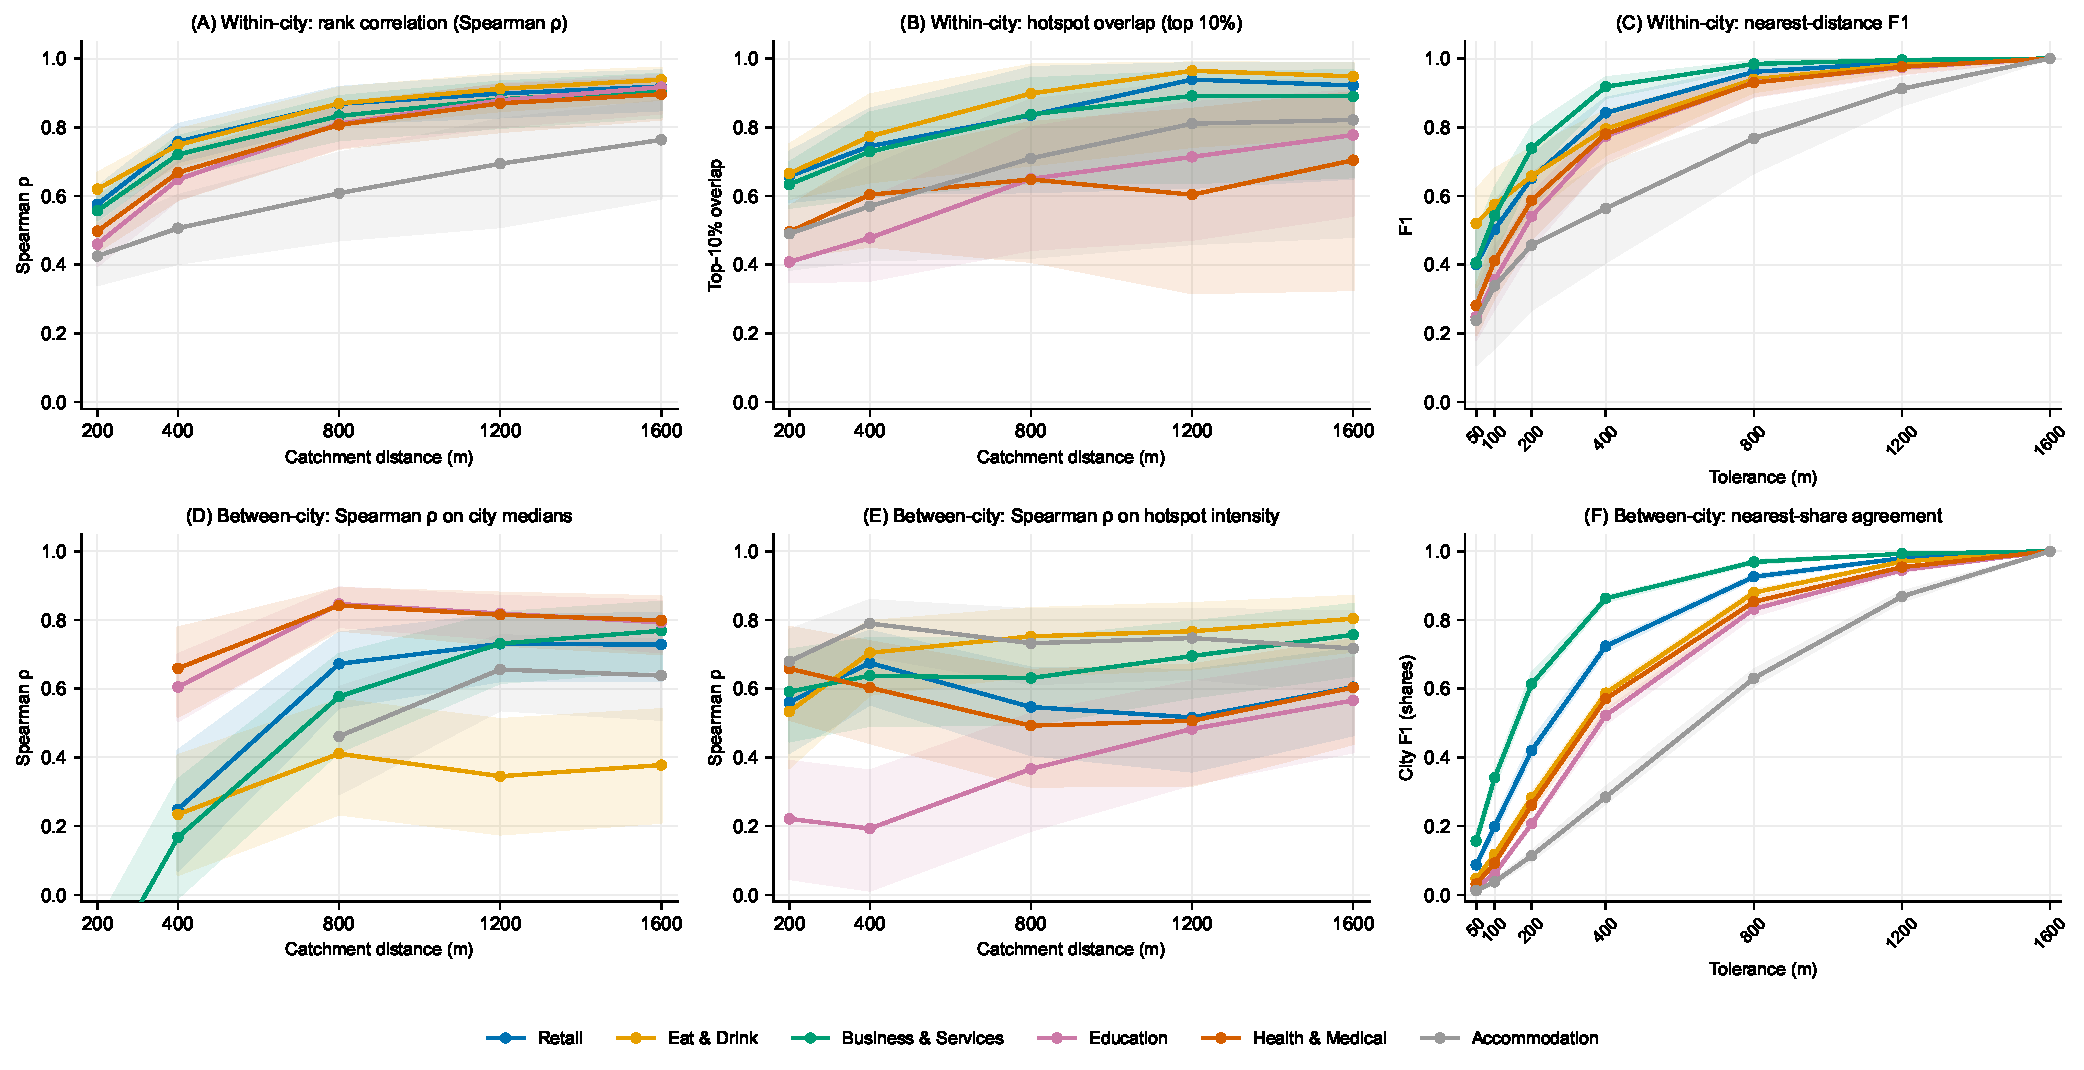
\includegraphics[width=\textwidth]{outputs/figures/fig_pointa_agreement_panels.pdf}
  \caption{\textbf{POI source-substitution agreement by category, task, and spatial scale.}
    \NRefCities{} reference cities. Top row (within-city): (A)~rank correlation (Spearman $\rho$), (B)~hotspot overlap, and (C)~nearest-within-tolerance F1; shaded bands show 95\% spatial block bootstrap CIs (distance-adaptive blocks, $B=200$). Bottom row (between-city): (D)~Spearman $\rho$ on city-level median counts, (E)~Spearman $\rho$ on city-level hotspot intensity, and (F)~harmonic-mean agreement of city-level nearest shares; shaded bands show 95\% city-level bootstrap CIs ($B=2{,}000$).
  }
  \label{fig:pointa_agreement_panels}
\end{figure}

\subsection{Per-city variability}
\label{sec:poi-supp-city-variability}

The main-text figures report median agreement across reference cities. Figure~\ref{fig:pointa_city_variability} shows the underlying per-city distributions at two representative catchment distances (400\,m and 800\,m). The strip plots confirm that the medians are not driven by a small number of outlier cities: at 800\,m most categories have tight distributions for rank correlation, with the bulk of cities exceeding 80\% concordance. Accommodation and Health \& Medical remain consistently the weakest categories with the widest spreads. Figure~\ref{fig:pointa_cross_city_scatter} complements this by plotting city-level median accessibility (log-transformed counts) from Overture against registry values at 800\,m; points falling below the identity line indicate systematic undercounting by Overture, particularly for Retail and Eat \& Drink.

\begin{figure}[p]
  \centering
  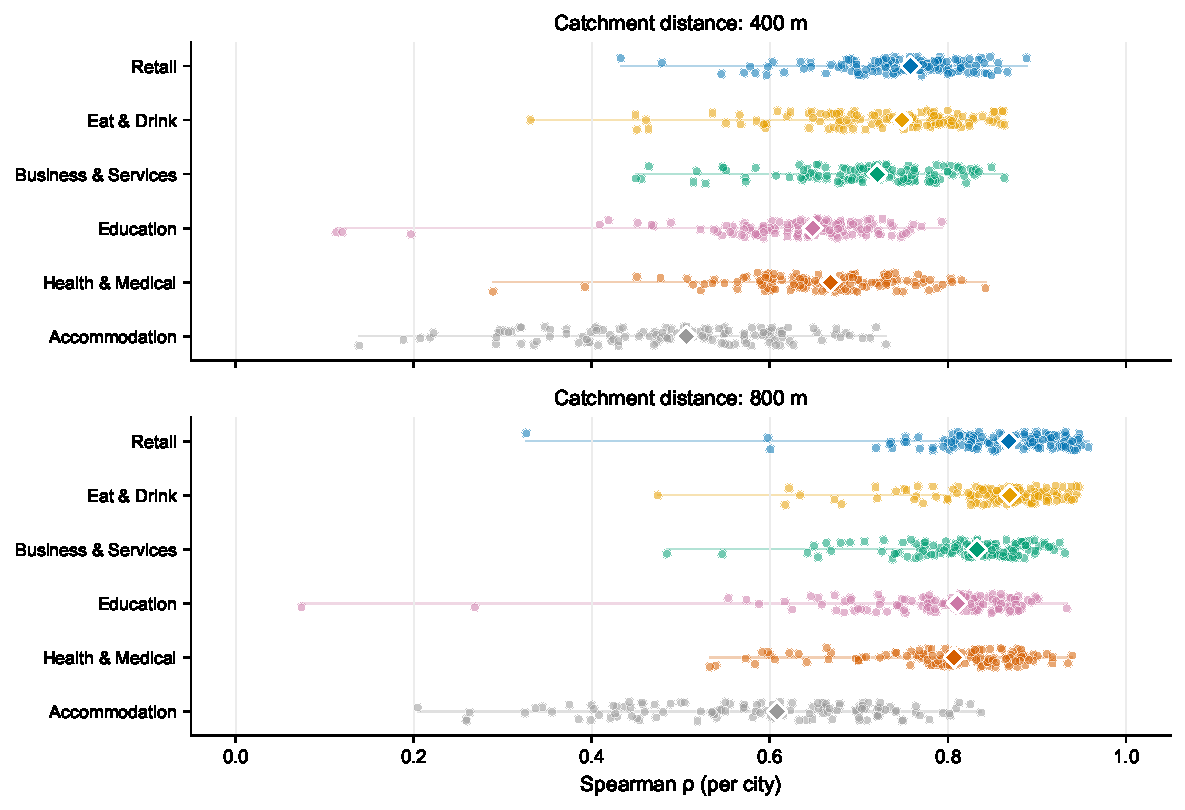
\includegraphics[width=0.88\textwidth]{outputs/figures/fig_pointa_city_variability.pdf}
  \caption{\textbf{Per-city rank correlation spread.}
    Distribution of Spearman $\rho$ (segment-level unweighted counts) across \NRefCities{} reference cities at 400\,m and 800\,m catchments. Points show individual cities; diamonds mark medians.
  }
  \label{fig:pointa_city_variability}

  \vspace{0.5em}

  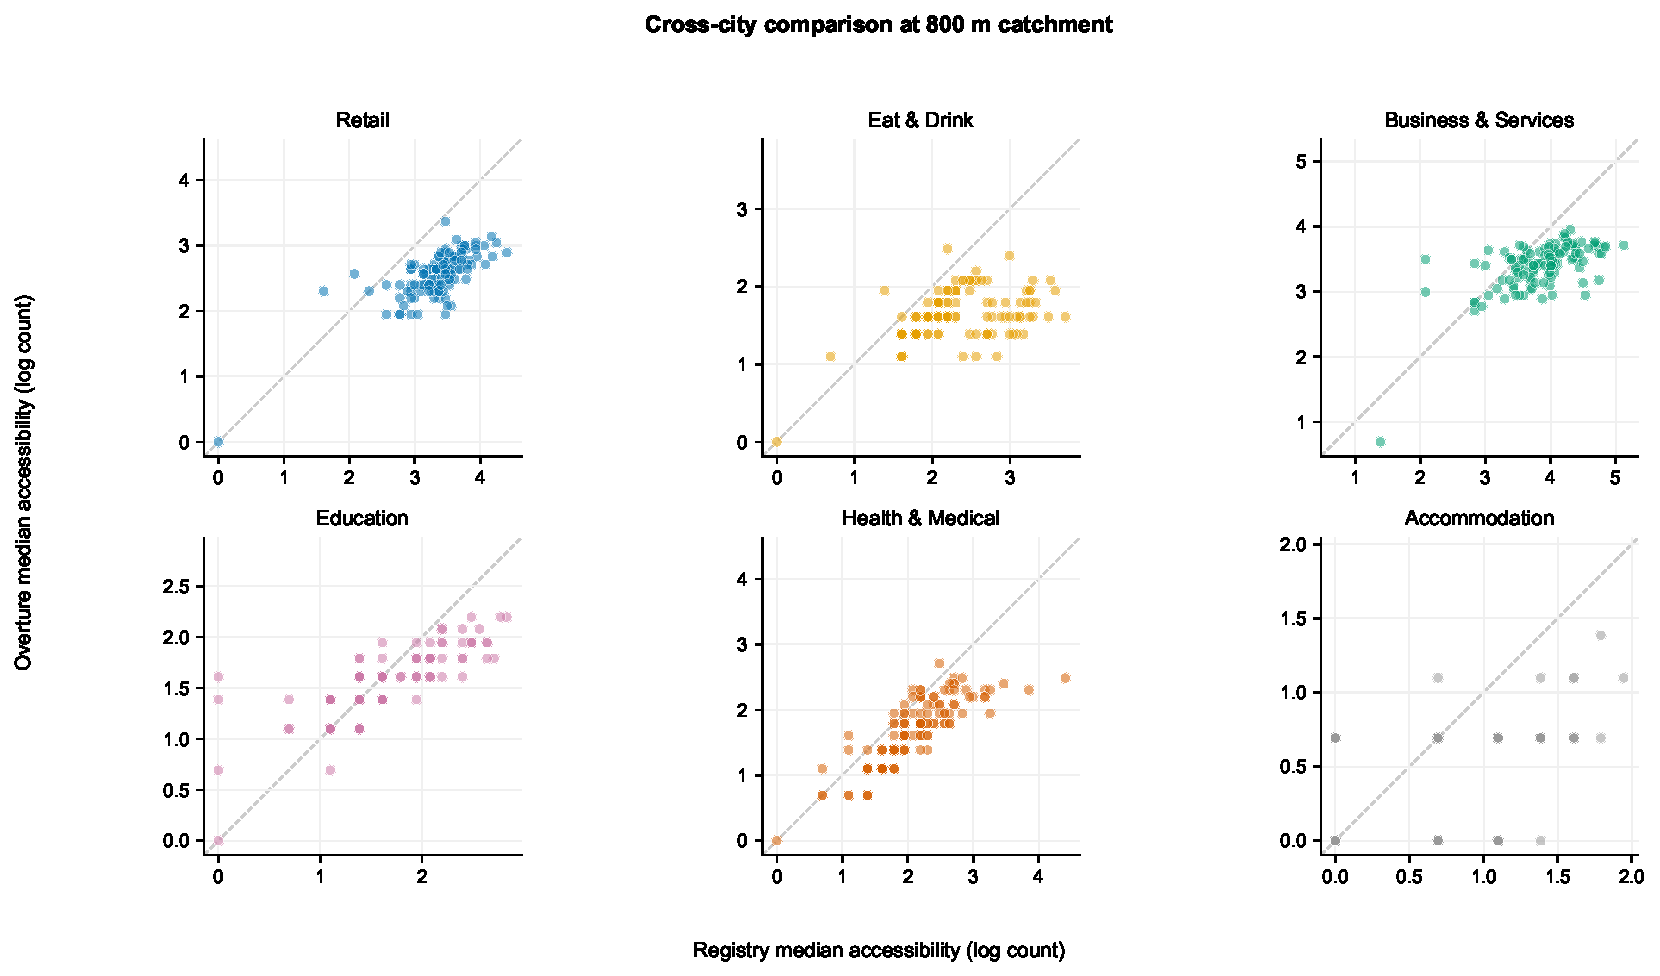
\includegraphics[width=0.88\textwidth]{outputs/figures/fig_pointa_cross_city_scatter.pdf}
  \captionof{figure}{\textbf{Cross-city comparison at 800\,m catchment.}
    Each point is one reference city. Axes show median log-transformed POI counts from registry and Overture sources; the dashed line marks identity. The predominance of points below the line indicates systematic undercounting by Overture, especially for Retail and Eat \& Drink.
  }
  \label{fig:pointa_cross_city_scatter}
\end{figure}

\subsection{Distance-weighted accessibility}
\label{sec:poi-supp-weighted}

The main-text results use unweighted POI counts (the number of establishments reachable within each catchment distance). An alternative is distance-weighted counts, where each POI's contribution decays with network distance, giving greater weight to nearer establishments.

At the same catchment distance, weighted counts produce lower concordance than unweighted counts (typically 3--5 percentage points for rank correlation, 5--8 for hotspot overlap), because the gravity weighting amplifies the effect of small geocoding offsets between sources. However, the weighted measure at 800\,m still exceeds the unweighted measure at 400\,m across all categories, since the larger catchment more than compensates for the concordance lost to weighting. This is relevant for applications that prefer distance-weighted accessibility: reliable concordance is achievable at 800\,m or above. The nearest-distance columns are unchanged, as they do not involve count aggregation.

\clearpage
\section{Building Footprint Source Composition and Metric Sensitivity}
\label{sec:bldg-supp}

This supplement documents the provenance composition of the Overture Maps building footprints used in SOAR-EU and quantifies its effect on derived morphometric indicators.

\subsection{Source classification}
\label{sec:bldg-supp-classification}

Each Overture building footprint carries a \texttt{sources} JSON array whose first element identifies the contributing dataset. We classify these into two groups: \emph{community-contributed} (OpenStreetMap, Esri Community Maps, national cadastral agencies) and \emph{ML-derived} (Microsoft ML Buildings, Google Open Buildings). Community-contributed footprints are digitised or imported from authoritative cadastral sources and generally preserve individual building boundaries; ML-derived footprints are segmented from satellite imagery and may merge adjacent buildings into single polygons or introduce unintended gaps between genuinely attached structures.

Across the \NCitiesTotal{} cities, the footprints draw on several source datasets: OpenStreetMap (dominant in most European cities), Esri Community Maps, Microsoft ML Buildings, and, in Spain, the Instituto Geogr\'{a}fico Nacional cadastre. Country-level aggregates reveal a clear geographic gradient (Table~\ref{tab:building_source_country}; Figure~\ref{fig:building_source_map}): the Netherlands, France, Switzerland, and Belgium are dominated by community sources, while Romania, Spain, Greece, and Bulgaria rely substantially on ML-derived footprints. The per-city ML fraction (Min and Max columns of Table~\ref{tab:building_source_country}) spans from zero in several cadastral-import cities to a large majority in the most ML-reliant. Per-city counts by dataset and country-level summaries are provided in the accompanying CSV files.

\begin{table}[!htb]
  \centering
  \caption{Building footprint source composition by country, sorted by ML-derived fraction (ascending). ML~(\%) is the proportion of footprints from ML-derived sources (primarily Microsoft ML Buildings); Min and Max show the per-city range within each country.}
  \label{tab:building_source_country}
  \scriptsize
  \input{outputs/tables/table_building_source_country}
\end{table}

\begin{figure}[!htb]
  \centering
  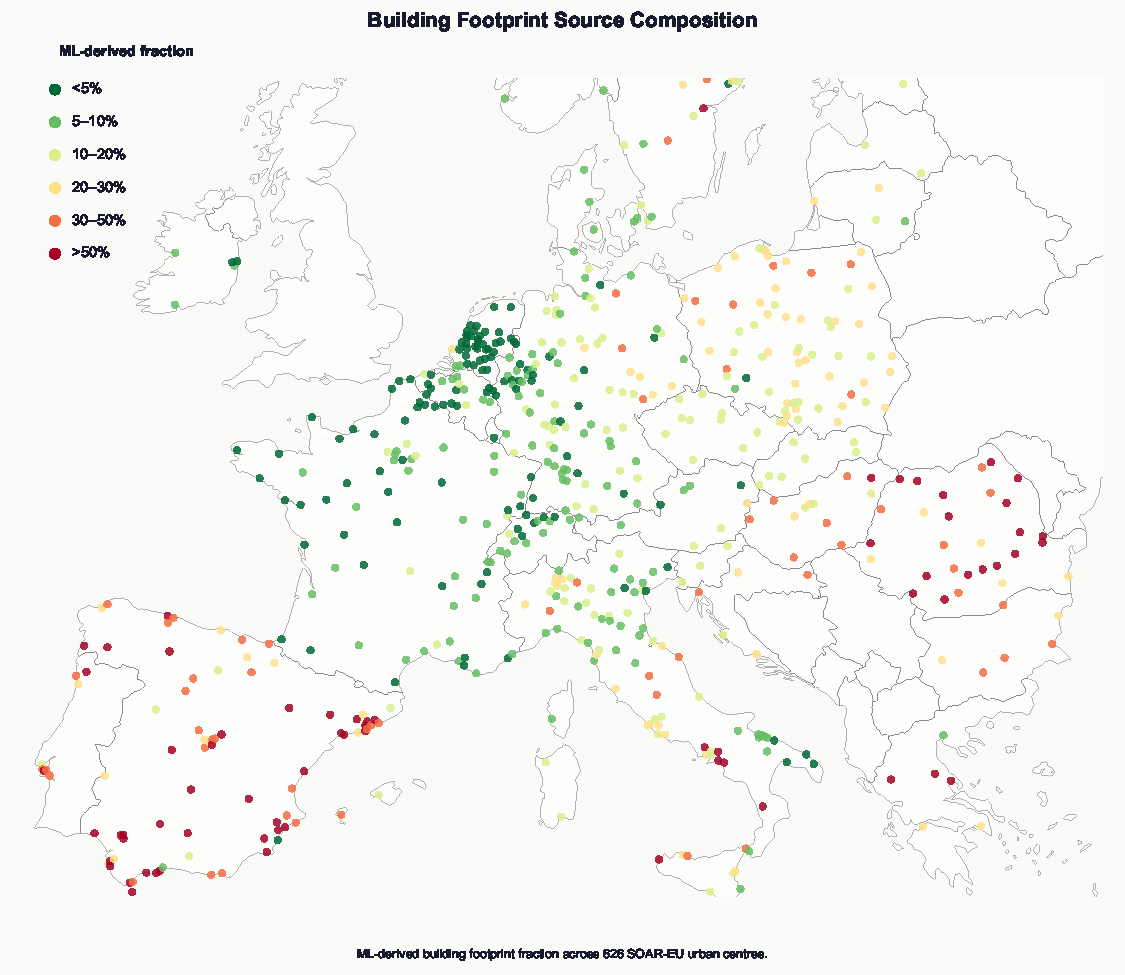
\includegraphics[width=\textwidth]{outputs/figures/fig_building_source_map.pdf}
  \caption{ML-derived building footprint fraction across the \NCitiesTotal{} SOAR-EU urban centres. Cities in western and northern Europe (France, Netherlands, Belgium, Germany) are dominated by community-contributed sources; cities in southern and eastern Europe (Romania, Spain, Greece, Bulgaria) rely more heavily on ML-derived footprints.}
  \label{fig:building_source_map}
\end{figure}

\subsection{Effect on morphometric indicators}
\label{sec:bldg-supp-sensitivity}

We test for source-driven bias at two levels.

\paragraph{Cross-city correlations.} For each morphometric indicator, we compute the Spearman correlation between each city's ML fraction and its median metric value across the \NCitiesTotal{} cities (Table~\ref{tab:building_metric_sensitivity}). Shared wall ratio shows the strongest negative association: cities with more ML-derived buildings have lower shared wall ratios. This cross-city correlation conflates two effects: a genuine morphological gradient (countries with higher ML fractions---Romania, Bulgaria, Greece---also have more freestanding housing stock) and a data artefact (ML-derived footprints underestimate shared walls due to polygon boundary gaps). The within-city test below isolates the artefact component. Perimeter, area, and volume are also positively associated, partly reflecting the tendency of ML segmentation to merge adjacent buildings into larger polygons and partly reflecting genuinely larger building footprints in lower-density settings. Fractal dimension and corner count show weaker but significant associations, while compactness, shape index, and orientation show no significant association with source composition.

\paragraph{Within-city comparisons.} To isolate the data artefact from genuine morphological differences between countries, we compare community and ML-derived buildings \emph{within the same city} using Mann-Whitney $U$ tests, restricted to cities containing both source types (Table~\ref{tab:building_metric_sensitivity}). Shared wall ratio shows a consistent within-city difference, significant in nearly all such cities: ML-derived buildings have lower shared wall ratios than community-contributed buildings in the same urban context, confirming a per-building artefact independent of cross-country morphological variation. Corner count and fractal dimension are also affected within cities, while compactness and shape index show small but widespread differences.

Block-level density metrics (GSI, FSI) show no meaningful cross-city association with ML fraction, likely because ML footprints add buildings in areas where community mapping is sparse, compensating for any area inflation from polygon merging. Table~\ref{tab:building_metric_sensitivity} summarises all cross-city and within-city results.

\begin{table}[!htb]
  \centering
  \caption{Sensitivity of building morphometric indicators to data source composition. Cross-city $\rho$: Spearman correlation between city ML fraction and city median metric value, across all \NCitiesTotal{} cities. Within-city $r$: median rank-biserial correlation from Mann-Whitney $U$ tests comparing community and ML-derived buildings within each city, restricted to cities containing both source types. Significance: {*}{*}{*}\,$p < 0.001$, {*}{*}\,$p < 0.01$, {*}\,$p < 0.05$.}
  \label{tab:building_metric_sensitivity}
  \scriptsize
  \input{outputs/tables/table_building_metric_sensitivity}
\end{table}

\subsection{Street-frontage ratio}
\label{sec:bldg-supp-frontage}

To provide a source-robust continuity measure, we compute a bilateral street-frontage ratio for each street segment. The computation proceeds as follows: (1)~buffer the street centreline by 35\,m to define a corridor (wide enough to capture building edges that address the street across a typical European front-garden or setback depth, narrow enough to exclude buildings on the next parallel street); (2)~identify all building edges whose midpoint falls inside the corridor and whose nearest street is this one (preventing cross-street contamination); (3)~classify each edge as left or right of the centreline using the local street tangent; (4)~per side, retain only edges within 5\,m of the closest edge, filtering out rear extensions and garages while preserving the primary facade line (5\,m is chosen to span typical facade step-ins and arcades without admitting rear-yard structures); (5)~project retained edges onto the centreline, merge overlapping intervals, and compute coverage as the fraction of street length covered (3\,m trimmed from each end as a junction guard, removing the short overlap where a corner property's facade would otherwise count toward both intersecting streets); (6)~the reported score (\texttt{frontage\_max}) is the maximum of the two sides. Per-side scores (\texttt{frontage\_left}, \texttt{frontage\_right}), their mean (\texttt{frontage\_avg}), and per-side edge counts (\texttt{frontage\_edges\_left}, \texttt{frontage\_edges\_right}) are also retained.

Unlike shared wall ratio, which requires exact topological contact between adjacent polygon boundaries, frontage ratio depends only on building \emph{presence} along the street edge. Whether two adjacent terraced houses are represented as separate touching polygons (community-digitised) or as a single merged polygon (ML-derived), the frontage coverage is the same. Across the \NCitiesTotal{} cities, the association between city-level ML fraction and median frontage ratio is substantially weaker than the corresponding shared-wall-ratio association (Table~\ref{tab:building_metric_sensitivity}). Because frontage is largely immune to the polygon-merging artefact that the within-city test identifies for shared wall ratio, this weaker residual association most likely reflects a predominantly genuine morphological gradient (countries with higher ML fractions also tend toward more freestanding housing) rather than a measurement artefact.

\end{document}
'
%
% If you hit a cryptic build error after edits (e.g., "Runaway argument" while
% writing labels/outlines), remove auxiliary files and rebuild:
%   rm -f manuscript.aux manuscript.out manuscript.toc manuscript.bbl manuscript.blg
%   pdflatex manuscript.tex && pdflatex manuscript.tex
\providecommand{\preprintmode}{0}
\newcommand{\IfPreprintTF}[2]{\ifnum\preprintmode=1\relax #1\else #2\fi}
\newcommand{\SpecsTableHeading}{\IfPreprintTF{Dataset summary}{Specifications Table}}
\newcommand{\ValueHeading}{\IfPreprintTF{Value of the dataset}{Value of the Data}}

% Submission placeholders (override at build time if desired)
\providecommand{\ZenodoDoi}{10.5281/zenodo.18961227}
\providecommand{\ZenodoUrl}{https://doi.org/10.5281/zenodo.18961227}
\providecommand{\GrantNumber}{101078890}

\usepackage[utf8]{inputenc}
\usepackage[margin=2.5cm]{geometry}
\usepackage{graphicx}
\usepackage{booktabs}
\PassOptionsToPackage{hyphens}{url}\usepackage{hyperref}
\usepackage{siunitx}
\usepackage{xcolor}
\usepackage{longtable}
\usepackage{multirow}
\usepackage{array}
\usepackage{float}        % Better float positioning
\usepackage{placeins}     % \FloatBarrier command
\usepackage{enumitem}     % Better list formatting
\usepackage{caption}      % \captionof for multi-figure floats
\usepackage{wrapfig}      % text-wrapping figures
\usepackage{amssymb}      % For \checkmark symbol
\usepackage{pdflscape}    % For landscape pages in supplementary

% Avoid hyperref warnings from elsarticle author-note macros in PDF strings
% (e.g., when writing metadata/bookmarks).
\makeatletter
\pdfstringdefDisableCommands{%
  \def\corref#1{}%
  \def\cnotenum{}%
  \def\@corref#1{}%
}
\makeatother

% Allow line breaks after underscores so long \texttt{} filenames
% (e.g. building\_source\_counts.csv) can wrap instead of overrunning the margin.
\renewcommand{\_}{\textunderscore\allowbreak}

% Auto-generated statistics macros (from paper_stats.json)
% Auto-generated LaTeX macros
% Generated by: python paper_data/code/s06_write_paper_macros.py
% DO NOT EDIT MANUALLY - regenerate from source data
% === City Counts ===
\newcommand{\NCitiesTotal}{626}
\newcommand{\NCountries}{28}
\newcommand{\NRefCities}{116}
\newcommand{\NRefCitiesFr}{73}
\newcommand{\NRefCitiesNl}{43}
\newcommand{\NNonRefCities}{510}

% === Data Coverage ===
\newcommand{\NCitiesLowHeight}{94}
\newcommand{\NCitiesNoHeight}{20}
\newcommand{\NCitiesWithHeightsRaster}{611}
\newcommand{\BldgHeightsAgeYears}{14}
\newcommand{\MedianHeightCoverage}{71}
\newcommand{\MedianBlockHundredCoverage}{74}
\newcommand{\NCitiesNoBlocks}{24}
\newcommand{\NCitiesNoEmployment}{185}

% === Dataset Size ===
\newcommand{\DatasetTotalCompressedGB}{35}
\newcommand{\DatasetMinMB}{3.5}
\newcommand{\DatasetMaxGB}{1.2}
\newcommand{\DatasetMeanMB}{56}

% === POI Validation Thresholds ===
\newcommand{\PoiNearDistGoodM}{800}
\newcommand{\PoiNearDistOtherM}{800}
\newcommand{\PoiNearDistAccomM}{1200}

% === Displacement Stats ===


% Consistent table column types
\newcolumntype{L}[1]{>{\raggedright\arraybackslash}p{#1}}
\newcolumntype{C}[1]{>{\centering\arraybackslash}p{#1}}
\newcolumntype{R}[1]{>{\raggedleft\arraybackslash}p{#1}}

\IfPreprintTF{}{\journal{Data in Brief}}

\begin{document}

\begin{frontmatter}

  \title{SOAR-EU: A Scalable, Open, Automatable, and Reproducible European Urban Dataset}

  \author[spacesyntax]{Gareth Simons\corref{cor1}}
  \ead{gareth.simons@ucl.ac.uk}
  \cortext[cor1]{Corresponding author}

  \author[spacesyntax]{Kayvan Karimi}
  \author[spacesyntax]{Sepehr Zhand}

  \affiliation[spacesyntax]{organization={Space Syntax Laboratory, UCL Bartlett School of Architecture},
    addressline={22 Gordon Street},
    city={London},
    country={United Kingdom}
  }

  \begin{abstract}
    Constructing spatial analytic datasets, particularly at scale, remains resource-intensive; SOAR-EU (Scalable, Open, Automatable, Reproducible --- European Urban) addresses this by providing ready-to-use pedestrian-scale urban metrics for \NCitiesTotal{} European cities across \NCountries{} countries to support comparative urban analytic research at the continental scale. Integrating GHS-UCDB urban boundaries, Eurostat census data, Copernicus Urban Atlas, and Overture Maps, it delivers over 100 pre-computed metrics per street at multiple spatial scales, covering network centrality, land-use and infrastructure accessibility, mixed-use diversity, building and block morphology, green-space and tree-canopy proximity, and demographics. Processing is automatable via open-source Python with fixed parameters; data are distributed as GeoPackage files in EPSG:3035. Because the Overture Maps POI layer aggregates commercial and editorial sources of varying completeness, we evaluate POI-derived accessibility through source-substitution replication against independent registries in \NRefCities{} reference cities in France and the Netherlands, providing task- and scale-specific guidance on when these metrics are more or less suitable for within-city pattern analysis and for broad between-city comparison.
  \end{abstract}

  \begin{keyword}
    pedestrian accessibility \sep
    street networks \sep
    land-use diversity \sep
    building morphology \sep
    walkability \sep
    cross-city comparison \sep
    spatial metrics
  \end{keyword}

\end{frontmatter}

%% ============================================================================
%% SPECIFICATIONS TABLE
%% ============================================================================
\section*{\SpecsTableHeading}

\begin{table}[!htbp]
  \centering
  \small
  \begin{tabular}{@{}L{3.2cm}L{8.3cm}@{}}
    \toprule
    \textbf{Subject} & Geography, Urban Studies, Geospatial Data Science \\
    \midrule
    \textbf{Specific subject area} & Urban morphology, pedestrian accessibility, land-use diversity \\
    \midrule
    \textbf{Type of data} & Table (geospatial vector); Processed, filtered (GeoPackage format) \\
    \midrule
    \textbf{Data format} & GeoPackage (.gpkg); one ZIP archive per country bundling the city GeoPackages, plus a boundary index file \\
    \midrule
    \textbf{How data was acquired} & Programmatic extraction and processing of open geospatial sources using Python (cityseer, momepy, GeoPandas). Metrics computed on natural street segments at multiple distance thresholds \\
    \midrule
    \textbf{Data collection} & Derived from publicly available authoritative sources: GHS-UCDB R2024A (2025 reference epoch), Overture Maps Foundation (2026 release), Copernicus Urban Atlas (2021), Copernicus Street Tree Layer (2021), Copernicus Height Model (2012), Eurostat Census Grid (2021) \\
    \midrule
    \textbf{Parameters for data collection} & Centrality thresholds: 400--9,600\,m. Accessibility thresholds: 200--1,600\,m. Morphology thresholds: 200--400\,m. CRS: EPSG:3035. See \href{https://github.com/UCL/t2e-soar-eu}{repository} for full configuration \\
    \midrule
    \textbf{Data source location} & Pan-European: \NCitiesTotal{} urban centres across 26 EU member states plus Norway and Switzerland (Liechtenstein has no qualifying urban centre under the GHS-UCDB threshold, and Cyprus is not covered by the GHS-UCDB R2024A European regional file used here). Coordinate Reference System: EPSG:3035 (ETRS89-LAEA Europe) \\
    \midrule
    \textbf{Data accessibility} & Repository: Zenodo. Data identification number: \ZenodoDoi{}. URL: \ZenodoUrl{} \\
    \midrule
    \textbf{Related research article} & G.\ Simons, K.\ Karimi, S.\ Zhand, A Morphological Atlas of European Urbanism: Eight Types of Urban Fabric Across Six Hundred Cities (SOAR-EU), submitted to \textit{Computers, Environment and Urban Systems}. \\
    \bottomrule
  \end{tabular}
\end{table}

%% ============================================================================
%% VALUE OF THE DATA
%% ============================================================================
\section*{\ValueHeading}

\begin{itemize}[leftmargin=*]
  \item The dataset enables \textbf{consistent comparative research} by removing the methodological confounds that usually frustrate cross-city work: all \NCitiesTotal{} cities are processed with identical methods, parameters, and source datasets, so measured differences reflect the urban fabric rather than differing analytical choices or bespoke data pipelines. This shared baseline supports benchmarking against continental norms, clustering streets into urban typologies, and detecting systematic differences in walkability and land use. Comparability is nonetheless bounded by the geographic consistency of the underlying open sources (Section~\ref{sec:provenance}): broad distributional comparison across regions and city groups is more strongly supported than exact city-by-city ranking, particularly for POI-derived metrics outside the validated French and Dutch reference set.
  \item The \textbf{multi-scale design} supports sensitivity analysis and scale-appropriate interpretation. Centrality metrics span 400\,m to 9,600\,m (5--120 minute walking catchments); accessibility metrics span 200\,m to 1,600\,m. Because relationships observed at one scale may not hold at others \cite{openshaw1984}, multiple thresholds are provided.
  \item The dataset supports \textbf{network-based accessibility} analysis that follows pedestrian routes rather than Euclidean buffers \cite{apparicio2008}. A park 200\,m as-the-crow-flies but 800\,m by foot is treated as 800\,m away. For each land-use category, both unweighted and distance-weighted counts are provided, supporting more nuanced aggregations in which proximity can be weighted by distance impedance.
  \item Researchers can benefit from the \textbf{fine-grained resolution} at street-segment level, which preserves within-neighbourhood heterogeneity and supports analysis from individual streets to city-wide patterns.
  \item The pipeline supports \textbf{reproducibility}: processing code and parameter settings are documented, enabling researchers to verify, regenerate, or extend the dataset as sources improve.
  \item The dataset benefits \textbf{urban planners, transport researchers, public health scientists, and environmental analysts} who need comparable pedestrian-scale indicators across European cities but lack the resources to assemble multi-source geospatial pipelines from scratch.
\end{itemize}

%% ============================================================================
%% OBJECTIVE
%% ============================================================================
\section*{Objective}

Comparative urban research requires consistent measurement across cities, yet constructing spatial analytic datasets remains resource-intensive. Related work includes GHSL \cite{pesaresi2023} global built-up surface mapping, Boeing's \cite{boeing2020} analysis of US street networks, Fleischmann et al.'s \cite{fleischmann2022} numerical taxonomy of urban form, and Yap and Biljecki's \cite{yap2023} feature-rich network dataset for 50 cities. Simons's \cite{simons2021thesis} pedestrian-scale integration of street networks, land use, and census demographics across 931 cities and towns in Great Britain is a direct methodological precursor to the present continental-scale dataset.

SOAR-EU (Scalable, Open, Automatable, Reproducible --- European Urban) complements these by providing ready-to-use pedestrian-scale metrics for \NCitiesTotal{} EU urban centres. The dataset integrates GHS-UCDB boundaries, Eurostat census grids, Copernicus land cover and building heights, and Overture Maps street networks and POIs. Metrics are computed on street segments across multiple spatial scales (200--9,600\,m) using the cityseer \cite{simons2023} Python package, spanning network centrality, land-use and infrastructure accessibility, mixed-use diversity, building and block morphology, green-space and tree-canopy proximity, and demographics. The pipeline is open-source and designed for regeneration as future data releases become available.

%% ============================================================================
%% DATA DESCRIPTION
%% ============================================================================
\section{Data Description}

\subsection{Dataset Structure}
\label{sec:dataset-structure}

The dataset comprises a \texttt{boundaries.gpkg} file derived from the GHS-UCDB urban centre boundaries, plus \NCountries{} country-level ZIP archives (\texttt{soar\_eu\_\{country\}.zip}) that bundle the \NCitiesTotal{} individually compressed city GeoPackages. Each city file follows the naming convention \texttt{metrics\_\{bounds\_fid\}.gpkg.zip}, where \texttt{bounds\_fid} corresponds to the unique identifier from \texttt{boundaries.gpkg}.

Each GeoPackage contains three layers: \textbf{streets} (natural street segments with computed metrics as LineString geometries), \textbf{buildings} (individual footprints with morphological attributes), and \textbf{blocks} (urban blocks with source and morphological attributes). The streets layer contains only \emph{live} segments (those whose midpoint falls within the urban centre boundary), excluding peripheral buffer segments used solely for edge-effect mitigation during network and accessibility analysis. Individual city files range from approximately \DatasetMinMB\,MB to \DatasetMaxGB\,GB depending on urban extent (average $\sim$\DatasetMeanMB\,MB); the complete compressed dataset is approximately \DatasetTotalCompressedGB\,GB. End-to-end processing takes approximately one day on a contemporary workstation-class laptop (18-core Apple M5 Pro).

Per-column completeness and building-source composition tables (\texttt{completeness\_coverage.csv}, \texttt{building\_source\_counts.csv}, and \texttt{building\_source\_by\_country.csv}) are bundled with the deposit; coverage is summarised in Section~\ref{sec:coverage} and source composition is interpreted in Section~\ref{sec:provenance}.

\subsection{Streets Layer}

The streets layer is the core of the dataset: each live segment carries pre-computed metrics spanning the full set of measure families: network centrality, land-use accessibility and mixed-use diversity, infrastructure accessibility, building and block morphology, green-space and tree-canopy proximity, and interpolated census demographics. Most are computed at several network-distance thresholds, indicated by a suffix (e.g., \texttt{\_400}, \texttt{\_800}). Table~\ref{tab:streets_schema} summarises the attribute groups; the complete per-column schema is given in Supplementary Material (Section~S1).

\begin{table}[!htbp]
  \centering
  \caption{Summary of streets layer attributes (selected metrics shown; full schema in Supplementary Material Section~S1).}
  \label{tab:streets_schema}
  \small
  \begin{tabular}{@{}L{4cm}L{8.1cm}@{}}
    \toprule
    \textbf{Attribute group} & \textbf{Description} \\
    \midrule
    \texttt{geometry}, \texttt{x}, \texttt{y} & Segment geometry and midpoint coordinates (EPSG:3035) \\
    \midrule
    \texttt{cc\_beta\_*} & Closeness centrality (gravity-weighted) at distance thresholds \\
    \midrule
    \texttt{cc\_harmonic\_*} & Harmonic closeness centrality \\
    \midrule
    \texttt{cc\_hillier\_*} & Hillier-type closeness (node count / mean distance) \\
    \midrule
    \texttt{cc\_farness\_*} & Farness (total network distance to reachable segments) \\
    \midrule
    \texttt{cc\_betweenness\_*} & Segment betweenness centrality \\
    \midrule
    \texttt{cc\_betweenness\_beta\_*} & Beta-weighted betweenness centrality \\
    \midrule
    \texttt{cc\_density\_*} & Street segment density within threshold \\
    \midrule
    \texttt{cc\_cycles\_*} & Network cycle count within threshold \\
    \midrule
    \texttt{cc\_\{landuse\}\_*\_nw} & Unweighted POI count for land-use category \\
    \midrule
    \texttt{cc\_\{landuse\}\_*\_wt} & Distance-weighted POI count for land-use category \\
    \midrule
    \texttt{cc\_\{landuse\}\_nearest\_max\_*} & Distance to nearest POI in category \\
    \midrule
    \texttt{cc\_\{infra\}\_*\_nw/wt} & Infrastructure accessibility: transport, parking, street-furniture counts \\
    \midrule
    \texttt{cc\_hill\_*} & Land-use diversity (Hill numbers $q=0,1,2$) \\
    \midrule
    \texttt{cc\_green\_nearest\_max\_*} & Distance to nearest green space \\
    \midrule
    \texttt{cc\_trees\_nearest\_max\_*} & Distance to nearest tree canopy \\
    \midrule
    \texttt{cc\_green\_area\_sum\_*}, \texttt{cc\_trees\_area\_sum\_*} & Green-space / tree-canopy area within threshold \\
    \midrule
    \texttt{cc\_*\_median\_*} & Building morphology, contextual aggregation (area, height, volume, compactness, shared-wall ratio, \ldots) \\
    \midrule
    \texttt{cc\_building\_*} & Building count within threshold \\
    \midrule
    \texttt{frontage\_max} & Bilateral street-frontage ratio: max(left, right) building coverage (0--1) \\
    \midrule
    \texttt{cc\_block\_*} & Contextual block morphology: area, perimeter, compactness, GSI, FSI, OSR, storeys, height \\
    \midrule
    \texttt{density}, \texttt{t}, \texttt{emp} & Interpolated census demographics (population, density, age, employment, nationality, migration) \\
    \bottomrule
  \end{tabular}
\end{table}

Two of these families, land-use and infrastructure accessibility, count points of interest grouped into analytical categories. The 11 land-use categories (\texttt{cc\_\{landuse\}\_*}) are listed in Table~\ref{tab:landuse} and the three infrastructure categories (\texttt{cc\_\{infra\}\_*}) in Table~\ref{tab:infrastructure}; both derive from Overture's classification as described in Section~\ref{sec:landuse-access}.

\begin{table}[!htbp]
  \centering
  \caption{Aggregated land-use categories derived from Overture Maps POI classification.}
  \label{tab:landuse}
  \small
  \begin{tabular}{@{}L{4.2cm}L{7.8cm}@{}}
    \toprule
    \textbf{Category} & \textbf{Includes} \\
    \midrule
    \texttt{eat\_and\_drink} & Restaurants, cafés, bars \\
    \texttt{retail} & Shops, supermarkets, pharmacies \\
    \texttt{business\_and\_services} & Automotive, beauty/spa, financial, home, professional services, real estate, travel agencies, pets, media, corporate offices \\
    \texttt{public\_services} & Government offices, libraries, civic facilities \\
    \texttt{health\_and\_medical} & Hospitals, doctors, dentists, optometrists \\
    \texttt{education} & Schools, universities, driving schools \\
    \texttt{accommodation} & Hotels, hostels, lodging \\
    \texttt{active\_life} & Sports facilities, fitness centres, recreation \\
    \texttt{arts\_and\_entertainment} & Cinemas, theatres, performance venues \\
    \texttt{attractions\_and\_activities} & Museums, landmarks, tourist attractions \\
    \texttt{religious} & Places of worship \\
    \bottomrule
  \end{tabular}
\end{table}

\begin{table}[!htbp]
  \centering
  \caption{Infrastructure categories derived from Overture Maps infrastructure theme.}
  \label{tab:infrastructure}
  \small
  \begin{tabular}{@{}L{3cm}L{9cm}@{}}
    \toprule
    \textbf{Category} & \textbf{Includes} \\
    \midrule
    \texttt{transport} & Bus stops, bus stations, railway stations, subway stations, ferry terminals, airports (including regional, international, seaplane), aerialway stations, helipads \\
    \texttt{street\_furn} & Benches, drinking water points, fountains, planters, plants, post boxes, picnic tables \\
    \texttt{parking} & Parking lots, motorcycle parking \\
    \bottomrule
  \end{tabular}
\end{table}

\subsection{Buildings and Blocks Layers}

The buildings layer contains individual building footprints derived from Overture Maps with morphological metrics including area, perimeter, compactness, orientation, estimated height (sampled from raster), volume, floor area, form factor, corners, shape index, shared wall ratio, and fractal dimension. Each footprint retains its Overture \texttt{sources} attribute, recording the contributing dataset (e.g., OpenStreetMap, Microsoft ML Buildings). The blocks layer provides urban block geometries derived from Urban Atlas with block-level morphology (area, perimeter, compactness, orientation, computed via the momepy package \cite{fleischmann2019}) and Spacematrix indicators: ground space index (GSI, building coverage ratio), floor space index (FSI), open space ratio (OSR), mean number of storeys (L), and area-weighted mean building height. Block-level morphology is reported only for built-up blocks; very small and oversized blocks are filtered out (appearing as NaN), with the thresholds and rationale given in Section~\ref{sec:metric-computation}.

\subsection{Coverage and Completeness}
\label{sec:coverage}

A per-column completeness report (\texttt{completeness\_coverage.csv}) is included with the dataset, listing the non-null coverage share for every attribute column in each city's streets, buildings, and blocks layers. Building footprint source composition is documented in \texttt{building\_source\_counts.csv} (per-city counts by source dataset) and \texttt{building\_source\_by\_country.csv} (country-level summaries); see Section~\ref{sec:provenance} for interpretation. Most metric groups (centrality, land-use and infrastructure accessibility, diversity, green-space and tree-canopy proximity, and building morphology) have near-complete coverage across all cities. Three categories exhibit variable coverage:

\begin{itemize}[nosep]
  \item \textbf{Height-derived metrics.} Building heights are sampled from the 2012 Copernicus Digital Height Model raster, whose spatial footprint does not cover all cities uniformly. Height-dependent attributes (mean height, volume, form factor, and their street-level contextual summaries) have a median coverage of \MedianHeightCoverage\%, with \NCitiesLowHeight{} cities below 50\% and \NCitiesNoHeight{} cities with no height data at all.\footnote{The \NCitiesNoHeight{}-city figure is derived per-column from \texttt{completeness\_coverage.csv}; it differs from the count of cities for which a Copernicus DHM raster was delivered at all (\NCitiesWithHeightsRaster{}/\NCitiesTotal{}) because some delivered rasters contain no usable pixels inside the city extent.}
  \item \textbf{Block morphology at 200\,m.} Contextual block metrics at the 200\,m threshold (area, perimeter, compactness, orientation, coverage ratio, and Spacematrix indicators) have a median coverage of \MedianBlockHundredCoverage\% (\NCitiesNoBlocks{} cities at zero). Coverage is reported over the filtered \emph{built-up} blocks layer that ships with each city file. Urban Atlas blocks classed as roads, rail, water, wetlands, agriculture, forest, green urban areas, sports/leisure, or otherwise exceeding 2\,km\textsuperscript{2} are excluded from urban morphological metrics (see Section~\ref{sec:metric-computation}), which particularly affects streets near city peripheries. The residual variability reflects a spatial scale effect: some street segments do not have any qualifying block within a 200\,m network radius. The same metrics at the 400\,m threshold have substantially higher coverage.
  \item \textbf{Employment.} Eurostat employment counts (\texttt{emp}, \texttt{emp\_\%}) are unavailable for \NCitiesNoEmployment{} cities, reflecting gaps in the upstream Census Grid. All other demographic variables (population, age structure, gender, nationality, migration) are near-universal.
\end{itemize}

\noindent The coverage report documents per-column coverage for each of these metric groups.

\subsection{Example Output}

Figure~\ref{fig:example-amsterdam} illustrates SOAR-EU output for Amsterdam, showing four representative metrics computed on the street network. Panel (A) shows closeness centrality at 800\,m, capturing network accessibility. Panel (B) shows retail catchment, the count of retail POIs reachable within 400\,m network distance, with higher values concentrated in the historic centre. Panel (C) shows distance to nearest green or blue space, indicating park and water proximity across the urban fabric. Panel (D) shows population density interpolated from the Eurostat Census Grid 2021 (1\,km\textsuperscript{2} resolution), expressed as persons per km\textsuperscript{2} of land surface. All metrics use network-based distances for aggregation, except for census statistics which are interpolated.

\begin{figure}[!htbp]
  \centering
  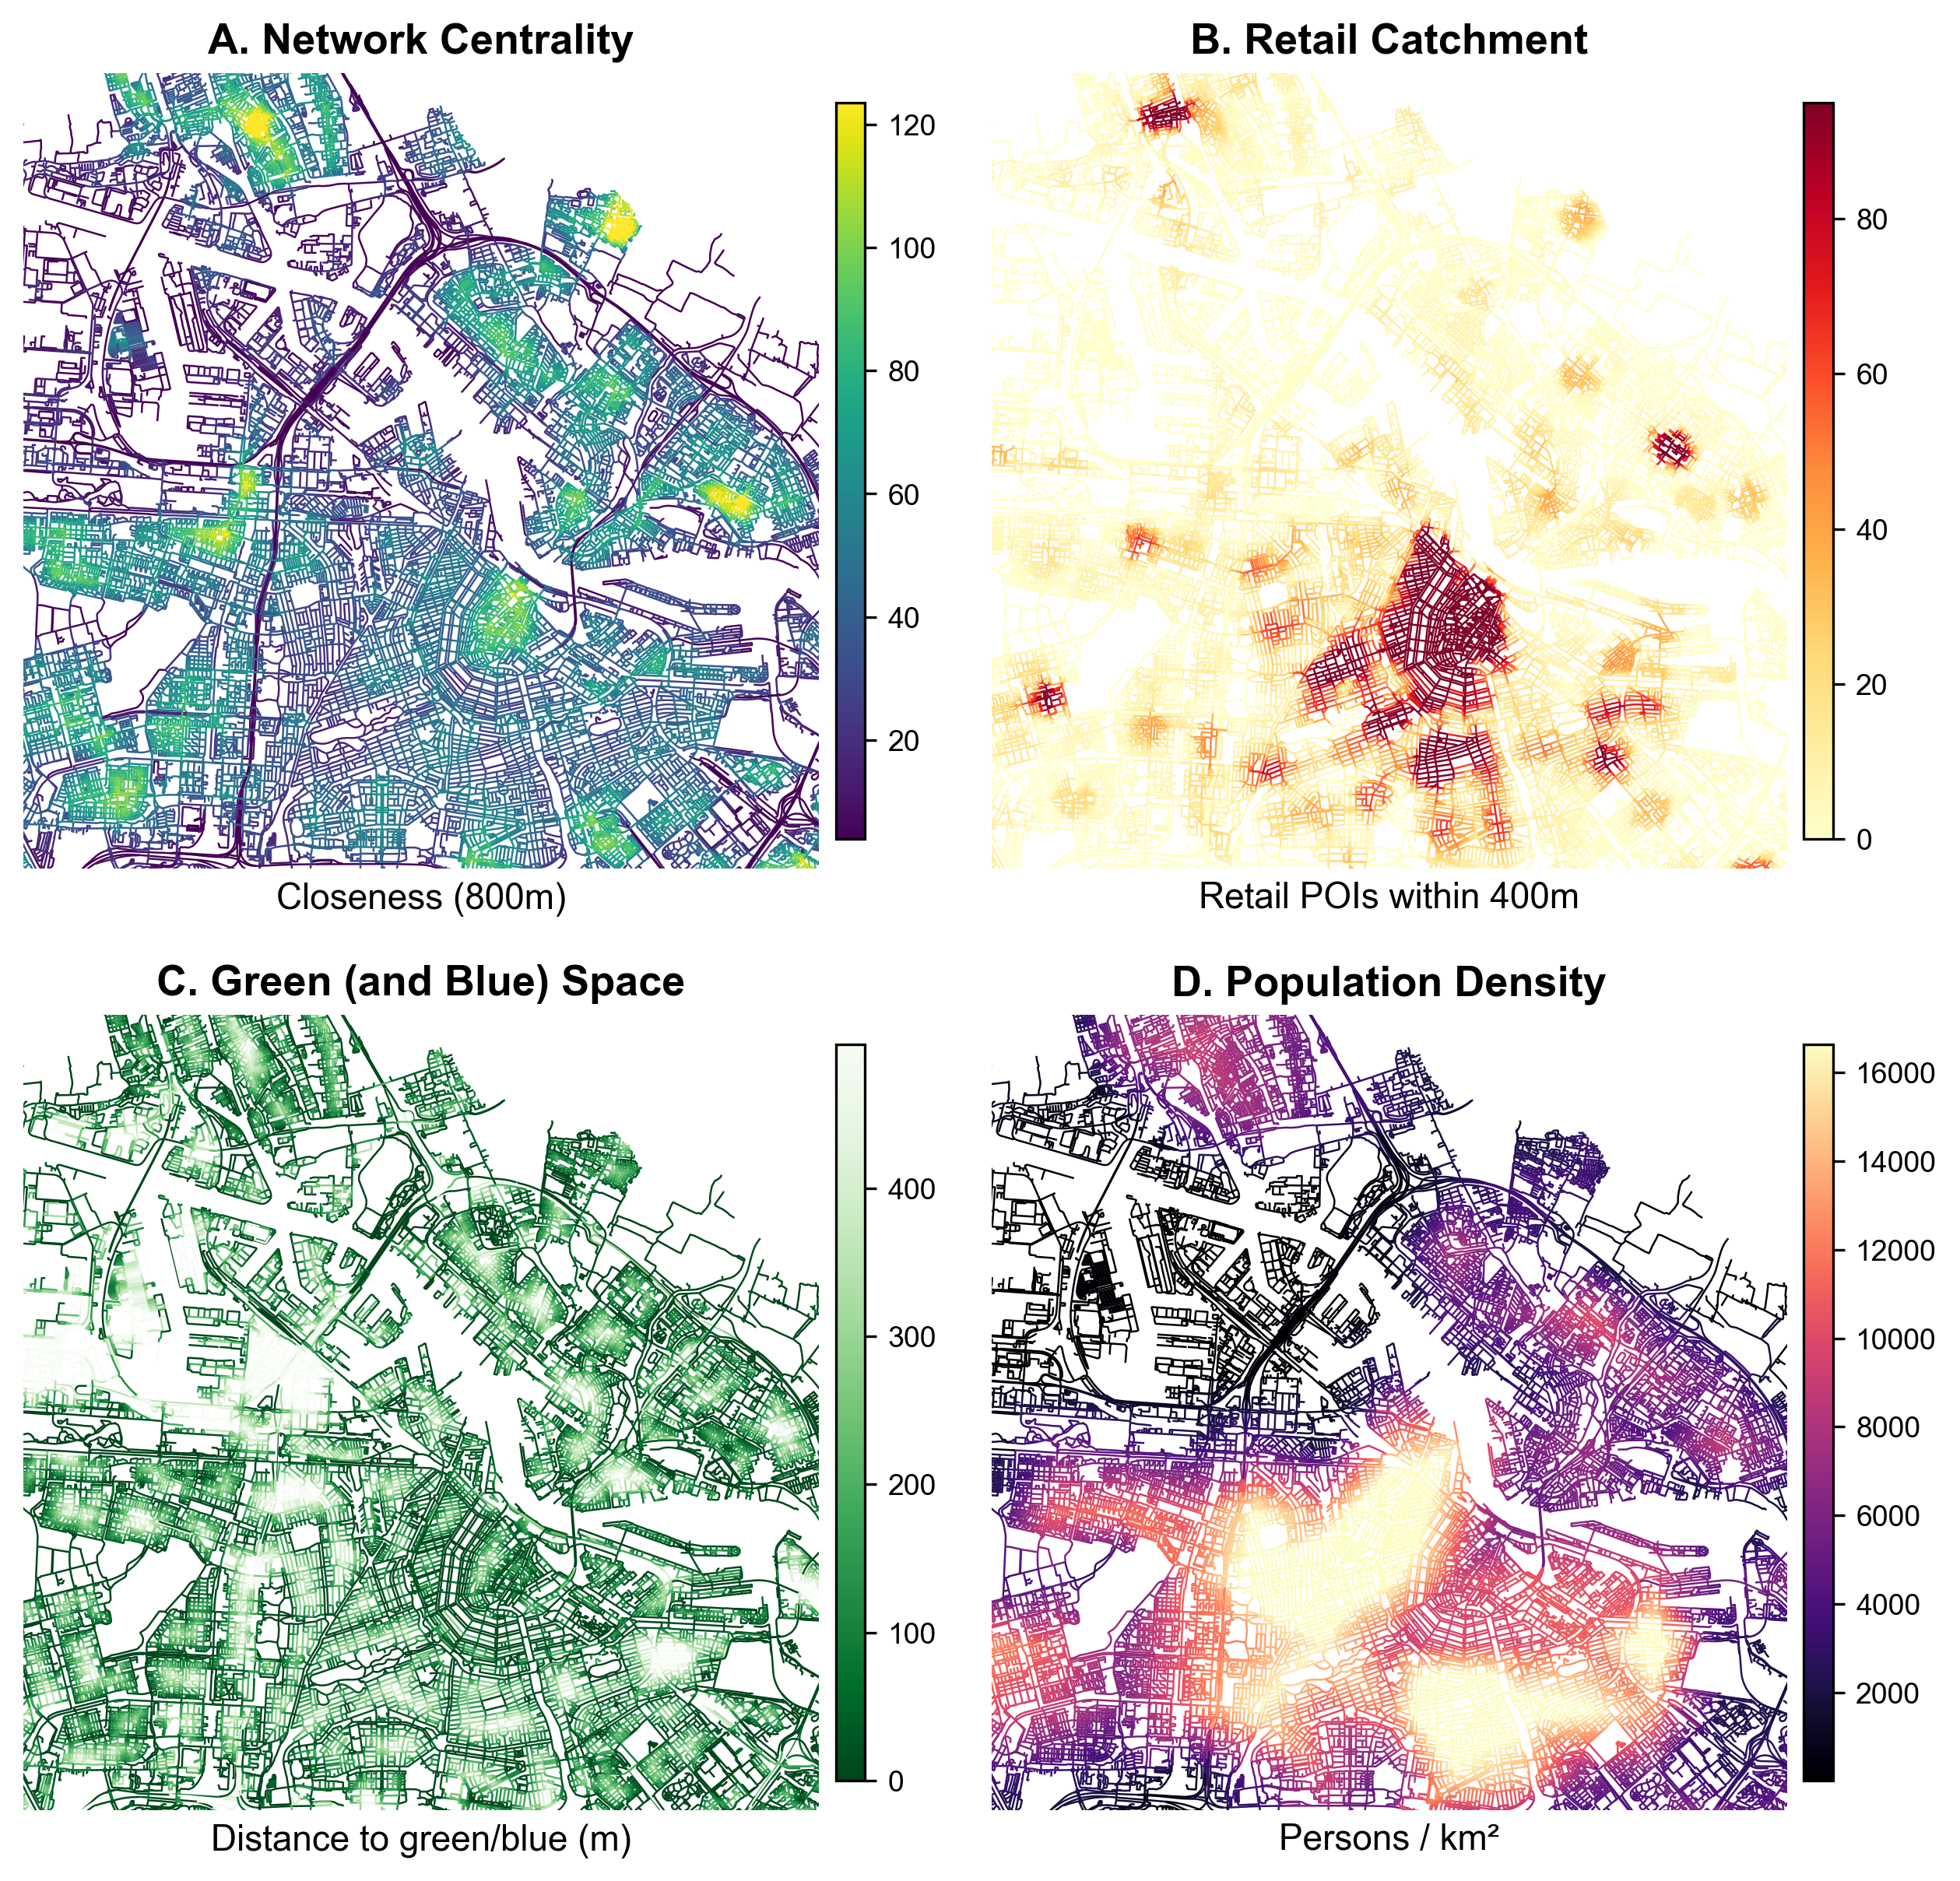
\includegraphics[width=\textwidth]{outputs/figures/fig_example_amsterdam.png}
  \caption{\textbf{Example SOAR-EU output for Amsterdam, Netherlands.} Street segments coloured by computed metrics: (A) closeness centrality at 800\,m threshold; (B) retail catchment (POI count within 400\,m); (C) distance to nearest green or blue space; (D) population density (persons/km\textsuperscript{2}, Eurostat Census Grid 2021). Different spatial scales and metric types lend themselves to different forms of analysis.}
  \label{fig:example-amsterdam}
\end{figure}

%% ============================================================================
%% METHODS
%% ============================================================================
\section{Methods}

Sections~\ref{sec:study-area}--\ref{sec:implementation} describe the processing pipeline (Figure~\ref{fig:pipeline}); Section~\ref{sec:provenance} discusses data provenance and source quality; Section~\ref{sec:poi-pattern-characterisation} provides scale-dependent usage guidance for POI-derived metrics. All source datasets were ingested during mid 2026 using the release versions indicated in Table~\ref{tab:sources}; the final dataset snapshot used for validation and distribution corresponds to Zenodo deposit \ZenodoDoi{}.

\begin{figure}[htbp]
  \centering
  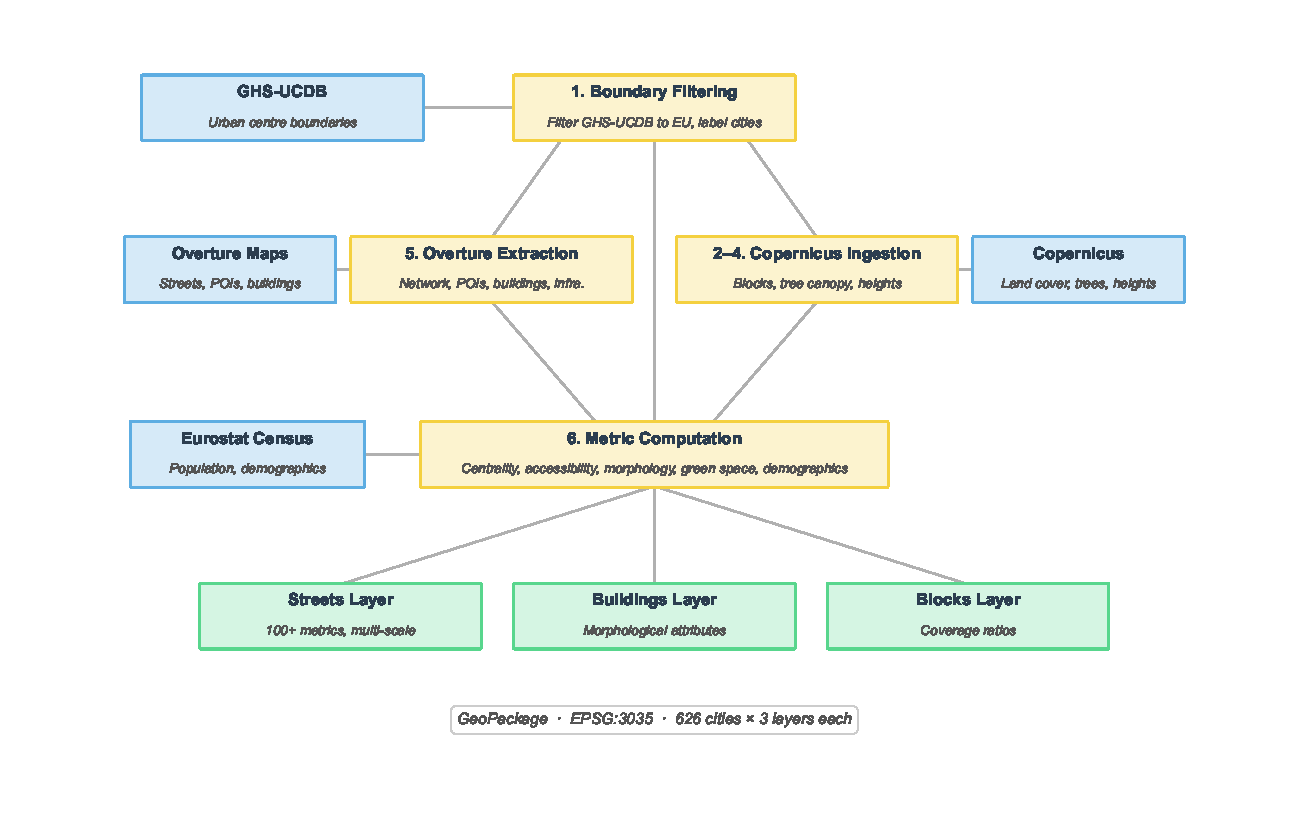
\includegraphics[width=0.85\textwidth]{outputs/figures/fig_pipeline.pdf}
  \caption{\textbf{SOAR-EU processing pipeline.} Four open data sources (blue) feed four processing stages (yellow) that produce three GeoPackage output layers per city (green). Stage~1 filters GHS-UCDB boundaries to the EU and labels cities; Stages~2--5 ingest Copernicus and Overture data in parallel; Stage~6 computes all metrics using the ingested layers, Eurostat census data, and the filtered boundaries.}
  \label{fig:pipeline}
\end{figure}

\subsection{Study Area Definition}
\label{sec:study-area}

Urban boundaries derive from the Global Human Settlement Layer Urban Centre Database (GHS-UCDB) R2024A \cite{ghsl2024}, which defines urban centres using the Degree of Urbanisation (DEGURBA) methodology: contiguous 1$\times$1~km grid cells with $\geq$1,500 inhabitants/km\textsuperscript{2} (or $\geq$50\% built-up surface) and cumulative population $\geq$50,000. Filtering to continental Europe (EPSG:3035) yielded \NCitiesTotal{} urban centres. All meet the $\geq$50,000 population threshold and thus correspond to cities or major urban agglomerations rather than small towns. City names are taken directly from the GHS-UCDB \texttt{GC\_UCN\_MAI\_2025} (Main Urban Centre Name) attribute. Because GHS-UCDB boundaries reflect population density contours rather than administrative units, assigned names may not always correspond to commonly used city names (e.g., a district name rather than the parent municipality).

\subsection{Data Sources}

Table~\ref{tab:sources} summarises input datasets.

Street networks from Overture Maps \cite{overture2026} were cleaned via cityseer \cite{simons2023}, following the automated network-cleaning procedure described in \cite{abdeldayem2026}: disconnected components were removed and degree-2 nodes collapsed. Level-aware processing prevents incorrect merging at bridges or tunnels. The 8\,m cleaning tolerance is deliberately conservative, prioritising consistent processing across all cities over city-specific fine-tuning.

POI categories from Overture's ``places'' theme were mapped to 11 analytical classes (Table~\ref{tab:landuse}; derivation in Section~\ref{sec:landuse-access}), and infrastructure points from Overture's infrastructure theme to three categories (transport, parking, street furniture; Table~\ref{tab:infrastructure}). Land cover and tree canopy derive from Copernicus Urban Atlas \cite{eea2021ua} and Street Tree Layer \cite{eea2021stl} respectively. Building heights were sampled from the Digital Height Model \cite{eea2012bh}.

Demographics from Eurostat Census Grid 2021 \cite{eurostat2024} include population, employment, age structure, nationality, and migration at 1~km\textsuperscript{2} resolution.

\begin{table}[H]
  \centering
  \caption{Input data sources and their roles in the processing pipeline.}
  \label{tab:sources}
  \small
  \begin{tabular}{@{}L{2.5cm}L{1.6cm}L{1cm}L{2.8cm}L{3.2cm}@{}}
    \toprule
    \textbf{Dataset} & \textbf{Source} & \textbf{Year} & \textbf{Licence} & \textbf{Use} \\
    \midrule
    GHS-UCDB R2024A & JRC/GHSL & 2024 & \href{https://commission.europa.eu/legal-notice_en\#copyright-notice}{EC reuse policy} & Urban boundaries \\
    Street networks & Overture Maps & 2026 & \href{https://opendatacommons.org/licenses/odbl/1-0/}{ODbL} & Centrality, accessibility \\
    Points of interest & Overture Maps & 2026 & \href{https://cdla.dev/permissive-2-0/}{CDLA-Permissive-2.0} & Land-use metrics \\
    Building footprints & Overture Maps & 2026 & \href{https://opendatacommons.org/licenses/odbl/1-0/}{ODbL} & Morphology \\
    Urban Atlas & Copernicus & 2021 & \href{https://land.copernicus.eu/en/data-policy}{Copernicus data policy} & Blocks, green space \\
    Street Tree Layer & Copernicus & 2021 & \href{https://land.copernicus.eu/en/data-policy}{Copernicus data policy} & Tree proximity \\
    Height Model & Copernicus & 2012 & \href{https://land.copernicus.eu/en/data-policy}{Copernicus data policy} & Building heights \\
    Census Grid & Eurostat & 2021 & \href{https://commission.europa.eu/legal-notice_en\#copyright-notice}{EC reuse policy} & Demographics \\
    \bottomrule
  \end{tabular}
\end{table}

\subsection{Data Processing Pipeline}

The pipeline comprises six stages executed via Python modules (Table~\ref{tab:pipeline}). All scripts support idempotent execution (existing outputs are skipped unless \texttt{overwrite} is specified), enabling incremental processing and failure recovery.

\begin{table}[H]
  \centering
  \caption{Processing pipeline stages with corresponding Python modules.}
  \label{tab:pipeline}
  \small
  \begin{tabular}{@{}cL{6cm}L{6cm}@{}}
    \toprule
    \textbf{Stage} & \textbf{Module} & \textbf{Description} \\
    \midrule
    1 & \texttt{src.data.generate\_boundary\_polys} & Filter GHS-UCDB boundaries to continental Europe \\
    2 & \texttt{src.data.load\_urban\_atlas\_blocks} & Extract Urban Atlas blocks per boundary \\
    3 & \texttt{src.data.load\_urban\_atlas\_trees} & Extract Street Tree Layer per boundary \\
    4 & \texttt{src.data.load\_bldg\_hts\_raster} & Clip building height rasters per boundary \\
    5 & \texttt{src.data.load\_overture} & Extract Overture data (network, POIs, buildings, infrastructure) \\
    6 & \texttt{src.processing.generate\_metrics} & Compute all metrics per boundary \\
    \bottomrule
  \end{tabular}
\end{table}

For accurate metric computation at boundary edges, input datasets are buffered beyond city boundaries. Street networks are buffered by 10\,km, giving nodes near boundaries a complete network context for centrality calculations. Points of interest, buildings, and infrastructure are buffered by 2\,km, capturing all reachable amenities for boundary-proximate locations. Copernicus land cover and tree canopy data is clipped to boundary bounding boxes for green-space proximity coverage.

\subsection{Metric Computation}
\label{sec:metric-computation}

\subsubsection{Network Centrality}
Network centrality metrics quantify a location's connectivity within the street network and were computed using the cityseer package \cite{simons2023}.

Closeness variants measure how accessible a location is relative to the rest of the network: beta-weighted closeness (gravity index with exponential distance decay), harmonic closeness (sum of inverse distances), Hillier-type closeness (node count divided by average node distance), farness (sum of distances), and street segment density. The density measure (\texttt{cc\_density\_DDD}) is an unweighted count of network nodes, each corresponding to a natural street-segment midpoint after cleaning, reachable within the network-distance threshold; it is not weighted by segment lengths. Betweenness centrality measures how often a location lies on shortest paths between other locations and is computed in both standard and distance-weighted forms.

Metrics were generated using cityseer's shortest-path centrality (\texttt{centrality\_shortest}) at thresholds of 400\,m, 800\,m, 1,200\,m, 1,600\,m, 4,800\,m, and 9,600\,m, corresponding to 5--120 minute walking catchments at 80\,m/min average pedestrian speed. These thresholds span local-to-global catchments: 400\,m captures immediate neighbourhood context; 800\,m reflects typical distances walked to transit; the 1,200--1,600\,m range corresponds to 15-minute walking catchments; 4,800\,m characterises district-scale network structure; and 9,600\,m extends to city-wide connectivity. Centralities are measured using shortest paths (as opposed to angular paths) for greater tolerance of artefacts deriving from automated street cleaning procedures.

\subsubsection{Land-Use and Infrastructure Accessibility}
\label{sec:landuse-access}
Points of interest from Overture Maps were classified into the 11 aggregated land-use categories distributed with the dataset (Table~\ref{tab:landuse}). The aggregation follows Overture's own top-level groupings to the extent possible, rather than imposing a re-engineered taxonomy: most of the 11 categories correspond directly to a single Overture top-level class, with only two consolidations (\texttt{eat\_and\_drink} merging restaurants, bars, and cafés; \texttt{business\_and\_services} merging eleven Overture professional and commercial sub-classes) and two renames (\texttt{public\_services} from \texttt{public\_service\_and\_government}, \texttt{religious} from \texttt{religious\_organization}). The complete mapping from Overture's 2,000+ leaf categories to analytical classes is detailed in Supplementary Material (Section~S2).

Overture's separate infrastructure theme is grouped into three further accessibility categories (transport, parking, and street furniture; Table~\ref{tab:infrastructure}), which receive the identical network-accessibility treatment described below.

Accessibility metrics aggregate POI counts over the street network at the same street-segment locations used for centrality computations, enabling direct comparison between network structure and land-use distribution \cite{simons2023}. Network-based distances are used throughout, rather than Euclidean buffers or zonal aggregation.

For each land-use and infrastructure category, both unweighted counts (reachable POIs within $d_{\max}$) and distance-weighted counts (applying exponential decay $e^{-\beta d}$, where $\beta = 4/d_{\max}$ such that weight falls to approximately 0.018 at the distance threshold) were computed, alongside nearest-distance measures. Distance-weighted counts reflect how amenity usage decays with distance (a caf\'{e} at 100\,m contributes more than one at 1,000\,m), while unweighted counts offer simpler interpretability.

The exponential weight never reaches zero, so an establishment infinitely far would still make an infinitesimal contribution. To keep each measure finite and tied to a walkable catchment, a threshold distance $d_{\max}$ is imposed rather than integrating over the entire network. The decay rate is set at $\beta = 4/d_{\max}$ where the weight has already fallen to under 2\% by the time it reaches $d_{\max}$, thereby discarding the infinitely long tail with minimal impact on the aggregations. The threshold distances are chosen for rounding convenience and the provision of a range of thresholds lets users choose the catchment that suits the intended usage scenario.

Mixed-use diversity was quantified using Hill numbers \cite{hill1973}. Hill numbers at $q=0$ equal richness (count of distinct land-use types); at $q=1$, the exponential of Shannon entropy; at $q=2$, the inverse Simpson index. We compute all three variants in both unweighted and distance-weighted forms, where the distance-weighted forms follow the same weighting conventions as described for land-use accessibility.

\subsubsection{Morphology}
Building and block morphology metrics were computed using the momepy package \cite{fleischmann2019}, which provides standardised urban morphometric functions.

For each building footprint, we compute: area, perimeter, circular compactness, orientation, corners count, shape index, fractal dimension, and shared wall ratio (fraction of perimeter shared with adjacent buildings). Building heights are extracted from the Copernicus Height Model raster by buffering each footprint by 10\,m (one DHM pixel) and averaging valid (non-null) overlapping pixel values. The single-pixel buffer ensures that small footprints (those contained within a single pixel) and footprints with minor misregistration against the 2012 raster still receive a height sample; the trade-off is some smoothing in dense fabric where party-wall neighbours and narrow courtyards fall within the buffer. The height value enables computation of volume and form factor. Floor area (assuming 3\,m floor height) is computed per building as an intermediate for block-level FSI but is not retained as a standalone aggregated metric.

Block morphology uses only built-up Urban Atlas blocks: 14 non-built land-cover classes (green areas, forests, agriculture, water, wetlands, and sports/leisure facilities) are excluded before morphometric computation and aggregation of the metrics to the adjacent streets. For the remaining blocks, we compute geometric properties (area, perimeter, circular compactness, orientation) and Spacematrix indicators \cite{haupt2010}: ground space index (GSI, building footprint area divided by block area), floor space index (FSI, total floor area divided by block area), open space ratio (OSR $= (1 - \text{GSI}) / \text{FSI}$), mean number of storeys (L $= \text{FSI} / \text{GSI}$), and area-weighted mean building height. Blocks exceeding 2\,km\textsuperscript{2} are additionally excluded as oversized infrastructural or transitional polygons (the threshold separates typical urban blocks from large airport, port, industrial, or transitional polygons that occur in the Urban Atlas layer); blocks below 1\% building coverage receive NaN for all Spacematrix metrics, since the ratios become numerically unstable as their denominators (GSI, FSI) approach zero.

Building and block metrics are aggregated to streets via nearest-network-distance assignment within 200\,m and 400\,m thresholds. Each building or block centroid is assigned to the nearest street, and statistics (median and median absolute deviation) are computed across all features within each threshold distance. For building area and volume, sum statistics are additionally retained; for block area, only the sum is additionally retained. Building height is also aggregated (as median and MAD of individual building heights per street).

In addition, a bilateral street-frontage ratio is computed per street segment as a source-robust measure of building continuity. For each street, a 35\,m buffer defines a corridor; all building edges whose midpoint falls inside the corridor and whose nearest street is this one are identified. Per side (left/right of the centreline), only edges within 5\,m of the closest edge are retained, filtering out rear extensions and garages while preserving the primary facade line. The score is the fraction of street length covered by the retained edges on the more-covered side (3\,m trimmed from each end as a junction guard). Unlike shared wall ratio, which requires exact topological contact between adjacent polygon boundaries, frontage ratio depends only on building \emph{presence} along the street edge. It is therefore insensitive to unintended gaps and to the lack of delineation between neighbouring buildings that is characteristic of ML-derived footprints, where segmentation pipelines lack the cadastral subdivision information available to community-contributed sources (see Section~\ref{sec:provenance}).

\subsubsection{Green Space Proximity}
Network distance to nearest green space polygon edge was computed for each street. Green spaces derive from 12 Urban Atlas land cover classes: public and unknown-access urban green areas, forests, herbaceous vegetation, open spaces with little or no vegetation, wetlands, water bodies, pastures, arable land, permanent crops, mixed cultivation, and orchards (full list in Supplementary Material Section~S3). Sports and leisure facility blocks often function as green space (e.g., open playing fields) but can also be heavily built up (e.g., stadiums, indoor arenas); we therefore apply a consistent 20\% building-coverage threshold, including the block as green space when built coverage is below 20\% and excluding it otherwise.

Polygon boundaries are sampled at 20\,m intervals to generate point features for distance calculations, improving accuracy for large or irregularly-shaped polygons. For each street, only the distance to the single nearest sampled point is retained, so a polygon contributes to a given street at most once regardless of how many of its boundary samples lie within range. Tree canopy proximity uses Street Tree Layer polygons with equivalent sampling. Green space and tree canopy areas are also aggregated within walking distances (200\,m, 400\,m, 800\,m) to quantify local coverage.

\subsubsection{Demographic Interpolation}
Census grid values were interpolated to street-segment midpoints using Delaunay-based linear barycentric interpolation (\texttt{scipy.interpolate.griddata}, method \texttt{linear}) from 1\,km grid cell centroids. Interpolated variables include: total population (\texttt{t}), population density (\texttt{density}), male/female counts (\texttt{m}, \texttt{f}), age cohorts (\texttt{y\_lt15}, \texttt{y\_1564}, \texttt{y\_ge65}), employment (\texttt{emp}), nationality (\texttt{nat}, \texttt{eu\_oth}, \texttt{oth}), and migration flows (\texttt{same}, \texttt{chg\_in}, \texttt{chg\_out}). Percentage variants (suffixed with \texttt{\_\%}) are computed for each variable relative to total population. Linear interpolation from 1\,km\textsuperscript{2} source cells produces smooth gradients that do not represent sharp sub-cell discontinuities (industrial estates, large parks, transit corridors); these street-level demographic values should be read as neighbourhood-scale context rather than as fine-grained block-level estimates.

\subsection{Implementation}
\label{sec:implementation}

The pipeline is implemented in Python 3.12 with modules for data ingestion, metric processing, utilities, and land-use classification. Network loading retrieves Overture ``connector'' and ``segment'' themes via STAC, transforms to EPSG:3035, and applies cityseer cleaning (8\,m tolerance, 100-node minimum component size). POI loading maps Overture's 2,000+ raw categories to 23 intermediate classes via a CSV lookup (preserved in the code repository for transparency and reuse), which are then aggregated to the 11 analytical categories distributed with the dataset (Table~\ref{tab:landuse}).

Table~\ref{tab:parameters} summarises the fixed processing parameters ensuring reproducibility across all urban centres.

\begin{table}[!htbp]
  \centering
  \caption{Fixed processing parameters for reproducibility.}
  \label{tab:parameters}
  \small
  \begin{tabular}{@{}L{4cm}L{3cm}L{4.5cm}@{}}
    \toprule
    \textbf{Parameter} & \textbf{Value(s)} & \textbf{Rationale} \\
    \midrule
    Network cleaning tolerance & 8\,m & Consolidate near-parallel edges \\
    Min.\ component size & 100 nodes & Remove disconnected fragments \\
    Centrality thresholds & 400, 800, 1200, 1600, 4800, 9600\,m & 5--120 minute walking catchments \\
    Accessibility thresholds & 200, 400, 800, 1200, 1600\,m & Pedestrian-scale proximity \\
    Morphology aggregation & 200, 400\,m & Immediate building context \\
    Green space proximity & 1600\,m & Extended walkable distance \\
    Green area aggregation & 200, 400, 800\,m & Multi-scale green coverage \\
    \bottomrule
  \end{tabular}
\end{table}

Outputs are written as GeoPackage files in EPSG:3035 following the structure described in Section~\ref{sec:dataset-structure}. Dependencies are pinned via \texttt{pyproject.toml}; core packages include cityseer, momepy, geopandas, and overturemaps.

\subsection{Data Provenance}
\label{sec:provenance}

SOAR-EU integrates data layers with different provenance. Eurostat boundaries, census data, and Copernicus land cover follow documented methodologies with full pan-European coverage. Street networks derive from OpenStreetMap via Overture, whose road coverage is largely complete across urbanised Europe \cite{barringtonleigh2017}.

Building footprints derive from Overture Maps, which conflates multiple sources in a fixed priority order: community-contributed datasets (OpenStreetMap, Esri Community Maps, national cadastres) take precedence over ML-derived datasets (Microsoft ML Building Footprints, Google Open Buildings). When two sources contain the same building (IoU~$\geq$~50\%), the higher-priority source's geometry is retained; ML-derived footprints fill areas not covered by community sources. Each footprint carries a \texttt{sources} attribute recording which dataset contributed it, enabling downstream filtering by provenance.

In European cities, OpenStreetMap is typically the dominant contributor. Herfort et al.\ \cite{herfort2023} analysed OSM building completeness across 13{,}189 urban agglomerations worldwide and found Europe and Central Asia to have the highest regional average (71\%), though within-region coverage remains uneven. Countries with completed cadastral imports---France (DGFiP cadastre), the Netherlands (BAG), and Belgium/Flanders (GRB)---are generally considered to have a high degree of community-sourced building coverage. In contrast, several southern and eastern European countries (including Romania, Bulgaria, Greece, Hungary, and Portugal) lack such imports and, in our data, rely more heavily on Microsoft's ML-derived footprints. Such ML-derived footprints overlap imperfectly with reference building data \cite{minghini2024}, as they are segmented from imagery rather than digitised from cadastre. Across the \NCitiesTotal{} cities in SOAR-EU, the proportion of ML-derived footprints ranges from near-zero in countries with complete cadastral imports to substantial in several southern and eastern European countries; per-city and per-country breakdowns are provided in the accompanying \texttt{building\_source\_counts.csv} and \texttt{building\_source\_by\_country.csv} (summarised in Supplementary~\S\ref{sec:bldg-supp}), and per-city completeness can be cross-referenced against the ohsome OSM-completeness map at \url{https://hex.ohsome.org/#/urban_building_completeness}.

ML-derived footprints expand coverage but introduce quality trade-offs relevant to morphometric computation. Because they are segmented from overhead imagery rather than digitised from cadastral plans, they delineate roof outlines rather than ground-level footprints and can merge adjacent structures into single polygons or leave gaps that break the topological adjacency these metrics rely on. The effect is visible directly in our data: metrics that depend on exact polygon boundary coincidence (particularly shared wall ratio and, to a lesser extent, fractal dimension) are systematically affected, with shared wall ratio showing the strongest negative association between a city's ML fraction and its median value (full coefficients in Supplementary Table~\ref{tab:building_metric_sensitivity}; the within-city test in Supplementary~\S\ref{sec:bldg-supp} confirms this as a per-building artefact rather than a country-level morphological gradient). Metrics based on polygon area and shape (compactness, orientation, shape index) show no significant association with source composition.

POI data derives primarily from commercial and editorial sources (e.g., Meta, Microsoft, Foursquare, OSM) via Overture, with variable coverage relative to official registries; this is characterised in detail in Section~\ref{sec:poi-pattern-characterisation}. Temporal currency and other cross-layer caveats are summarised under Limitations of the Dataset.

\subsection{POI-derived accessibility: source-substitution analysis}
\label{sec:poi-pattern-characterisation}

Because Overture's POI layer aggregates commercial and crowdsourced data of varying completeness, the reliability of derived metrics varies across categories and spatial scales. To characterise where agreement holds and where it does not, we recompute POI-derived outputs against independent official registries in the two countries for which suitable national registries are openly available: France (SIRENE, \NRefCitiesFr{} cities) and the Netherlands (BAG, \NRefCitiesNl{} cities), \NRefCities{} reference cities in total. This validation therefore speaks directly to French and Dutch coverage; cities elsewhere in Europe (particularly in southern and eastern Europe, where OpenStreetMap-derived coverage is less mature) are outside its scope and should be treated with the additional caution discussed under Limitations of the Dataset. We frame the comparison around three questions that capture the main analytical uses of the resulting metrics:
\begin{itemize}
  \item \textbf{How many, relative to elsewhere?} Whether locations are ranked consistently by how much of a particular land use they can access. This is a pattern-agreement question as opposed to one of absolute counts: Overture is known to undercount relative to official registries (further discussed below), so the analytically useful question is whether that undercounting preserves the spatial ordering of accessibility.
  \item \textbf{Where are the hotspots?} Which locations fall in the top tier of activity.
  \item \textbf{How far is the nearest?} Whether the land use is reachable within a given distance threshold.
\end{itemize}
For each question, we measure agreement between Overture- and registry-derived accessibility for every street segment, then summarise within cities and across cities for each category and spatial scale (Figure~\ref{fig:pointa_support_heatmap}; Table~\ref{tab:pointa_minima}).

\subsubsection{Source-substitution replication}

\begin{figure}[!htb]
  \centering
  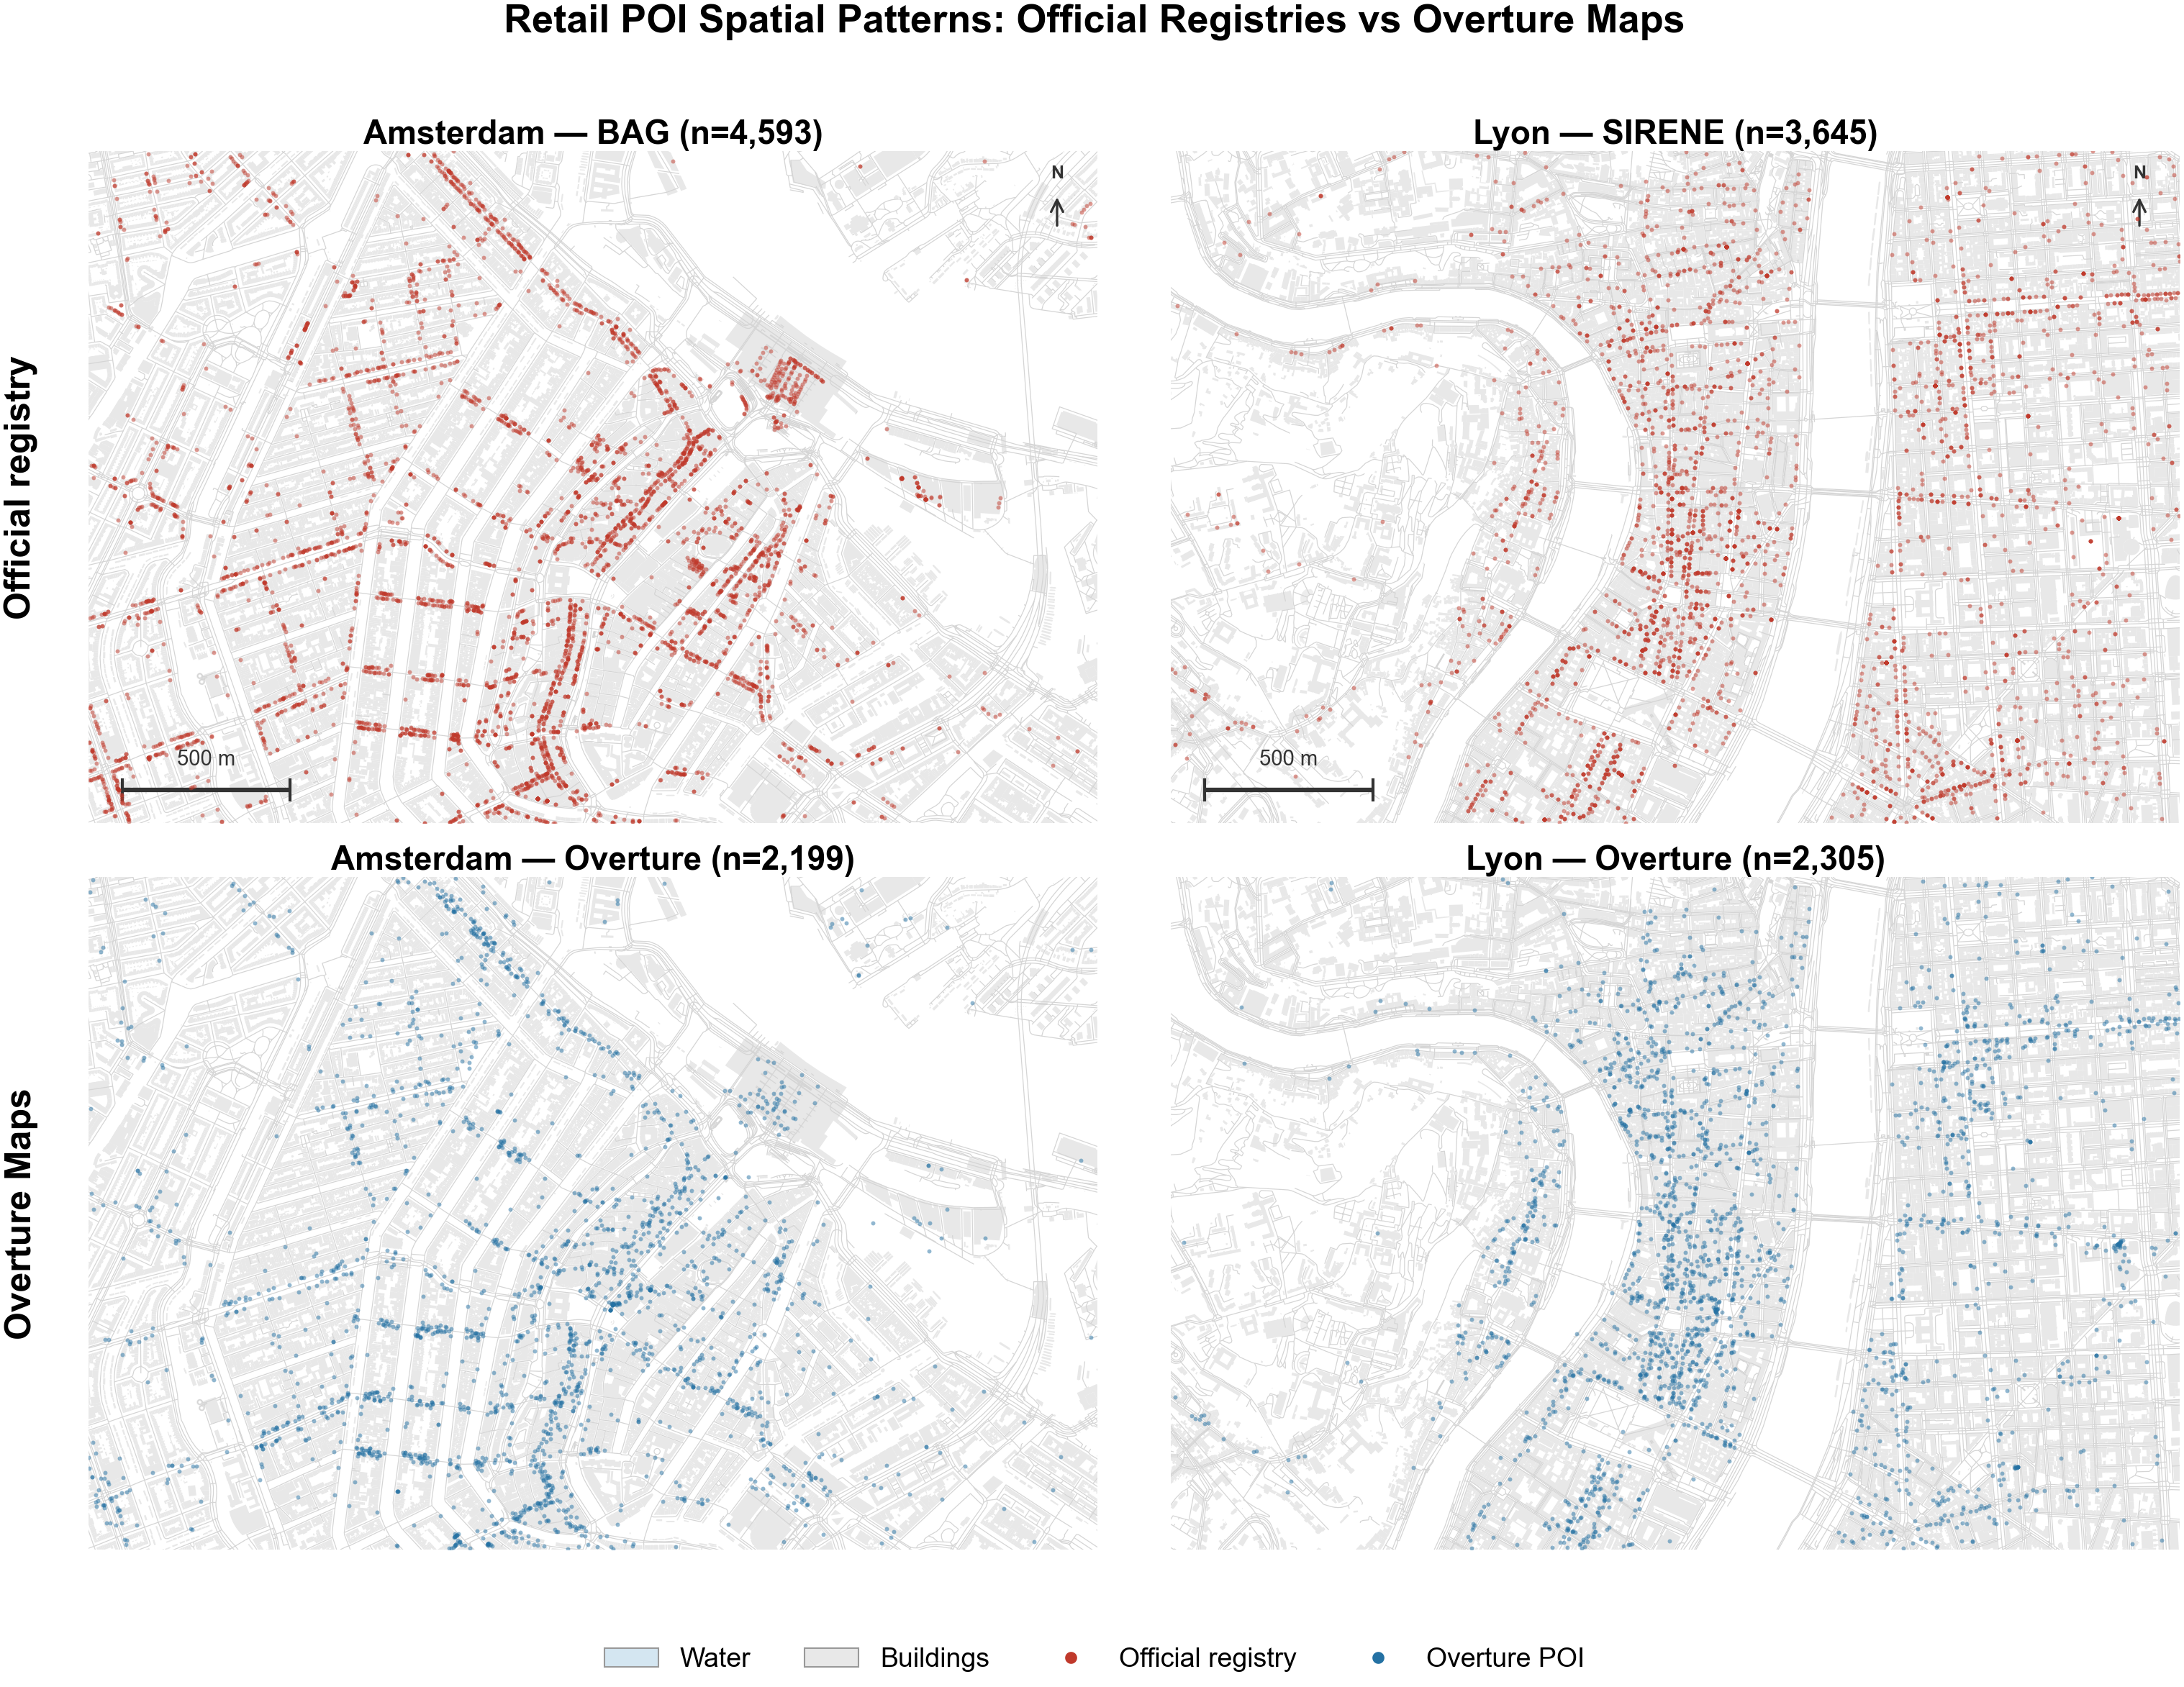
\includegraphics[width=\textwidth]{outputs/figures/fig_poi_spatial_comparison.png}
  \caption{\textbf{Retail POI locations from official registries (top) and Overture Maps (bottom)} for inner-city areas of Amsterdam (BAG; left) and Lyon (SIRENE; right). Point counts differ substantially between sources (Overture undercounts relative to the official registries), but the spatial clustering patterns are broadly consistent.}
  \label{fig:poi_spatial_comparison}
\end{figure}

\begin{figure}[p]
  \centering
  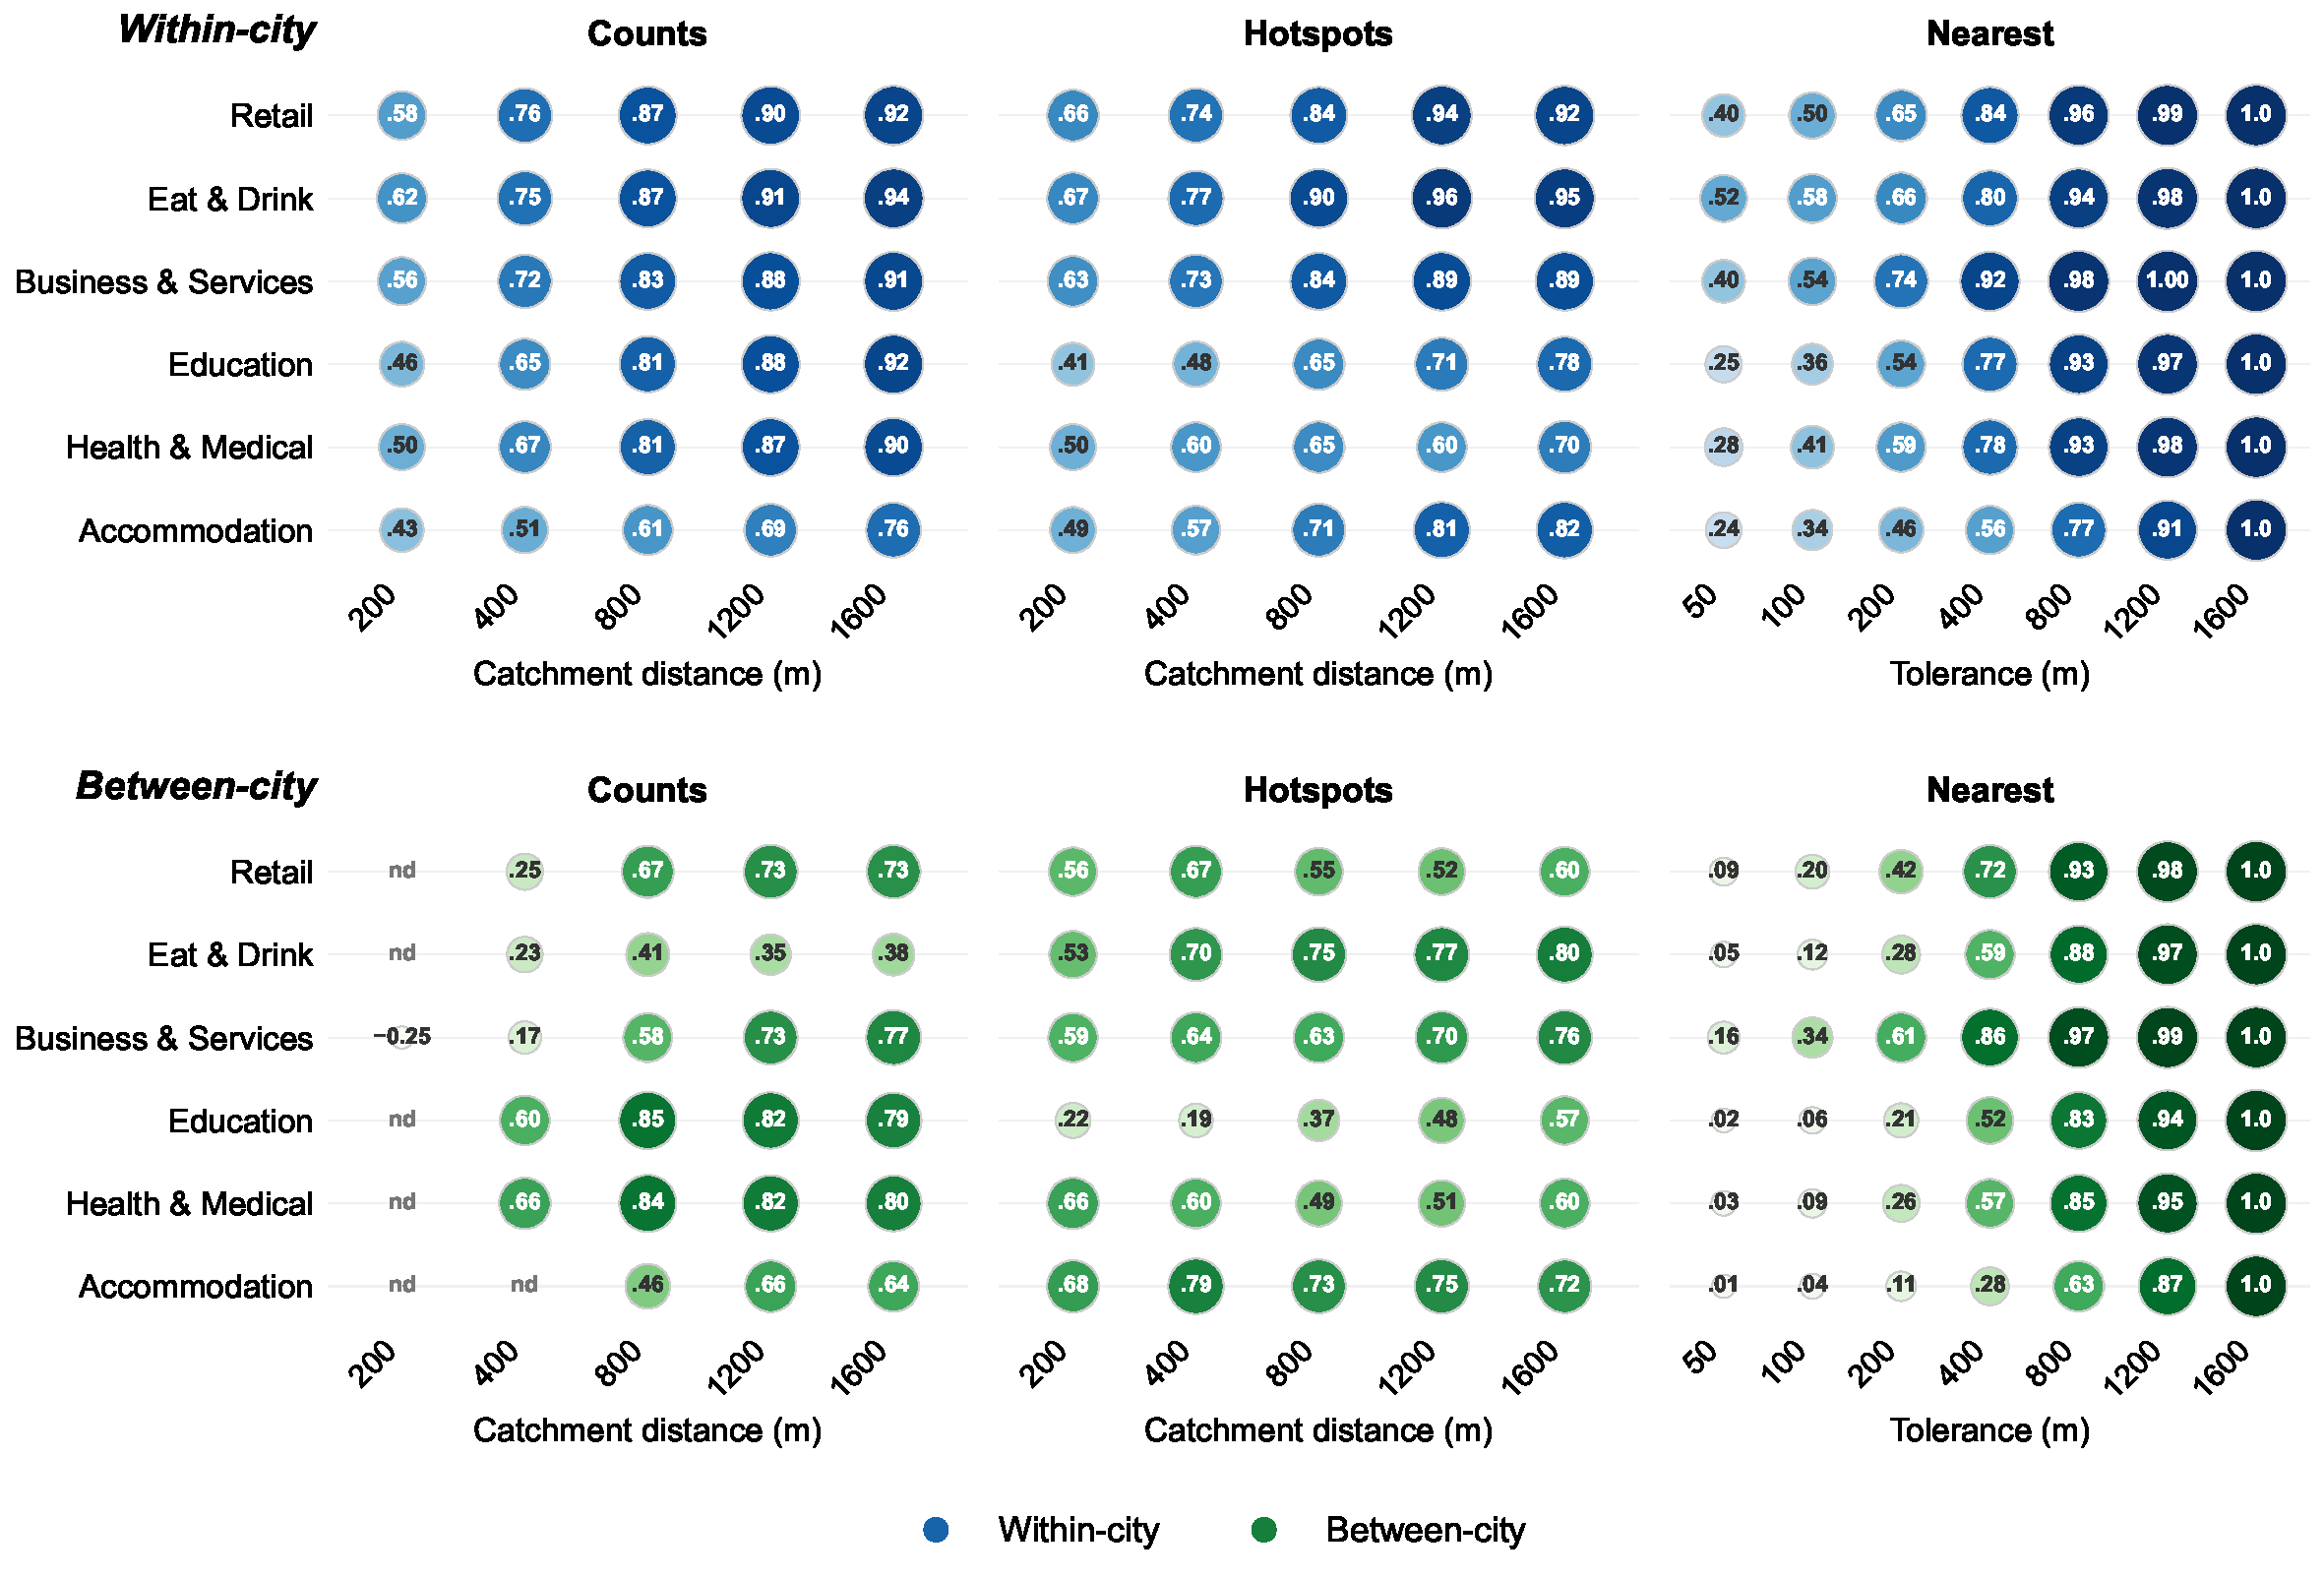
\includegraphics[width=\textwidth]{outputs/figures/fig_pointa_support_heatmap.pdf}
  \caption{\textbf{POI source-substitution agreement.}
    Agreement between Overture- and registry-based accessibility across all category--task--scale combinations. Top row (within-city): Spearman $\rho$ for segment-level rank correlation, top-10\% hotspot overlap, and nearest-distance F1. Bottom row (between-city): Spearman $\rho$ on city-level median counts and hotspot intensity, and harmonic-mean agreement of city-level nearest shares. Bubble size and annotation indicate the median score; colour distinguishes within-city from between-city scope. ``nd'' indicates insufficient data. Full agreement curves with bootstrap CIs appear in Supplementary Figure~\ref{fig:pointa_agreement_panels}.
  }
  \label{fig:pointa_support_heatmap}
\end{figure}

\begin{table}[p]
  \centering
  \caption{Minimum spatial scale (metres) at which each category's median agreement reaches $\geq$70\%, $\geq$75\%, $\geq$80\%, and $\geq$85\% concordance, grouped by scope (within-city, between-city) and metric family. For rank-correlation metrics, concordance is the fraction of observation pairs ranked identically by both sources, computed directly as $(1+\tau)/2$ where $\tau$ is the Kendall rank correlation (thresholds: $\tau \geq 0.40$, $0.50$, $0.60$, $0.70$). For overlap and F1 metrics the concordance fraction is used directly. Dashes indicate no tested scale reached that value.}
  \label{tab:pointa_minima}
  \scriptsize
  \begin{tabular}{@{}lcccccccccccc@{}}
\toprule
\textbf{Category} & \multicolumn{4}{c}{\textbf{Counts}} & \multicolumn{4}{c}{\textbf{Hotspots}} & \multicolumn{4}{c}{\textbf{Nearest}} \\
\cmidrule(lr){2-5}
\cmidrule(lr){6-9}
\cmidrule(lr){10-13}
 & $\geq$70\% & $\geq$75\% & $\geq$80\% & $\geq$85\% & $\geq$70\% & $\geq$75\% & $\geq$80\% & $\geq$85\% & $\geq$70\% & $\geq$75\% & $\geq$80\% & $\geq$85\% \\
\midrule
\textit{Within-city} & \multicolumn{4}{c}{\footnotesize rank concordance} & \multicolumn{4}{c}{\footnotesize top-10\% overlap} & \multicolumn{4}{c}{\footnotesize nearest F1} \\
Retail & 200 & 200 & 400 & 800 & 400 & 800 & 800 & 1200 & 400 & 400 & 400 & 800 \\
Eat \& Drink & 200 & 200 & 400 & 800 & 400 & 400 & 800 & 800 & 400 & 400 & 800 & 800 \\
Business \& Services & 200 & 400 & 800 & 1200 & 400 & 800 & 800 & 1200 & 200 & 400 & 400 & 400 \\
Education & 200 & 400 & 800 & 1200 & 1200 & 1600 & --- & --- & 400 & 400 & 800 & 800 \\
Health \& Medical & 200 & 400 & 800 & 1200 & 1600 & --- & --- & --- & 400 & 400 & 800 & 800 \\
Accommodation & 200 & 800 & 1600 & --- & 800 & 1200 & 1200 & --- & 800 & 800 & 1200 & 1200 \\
\midrule
\textit{Between-city} & \multicolumn{4}{c}{\footnotesize rank concordance (city medians)} & \multicolumn{4}{c}{\footnotesize rank concordance (hotspot intensity)} & \multicolumn{4}{c}{\footnotesize harmonic-mean share} \\
Retail & 800 & 800 & --- & --- & 200 & --- & --- & --- & 400 & 800 & 800 & 800 \\
Eat \& Drink & --- & --- & --- & --- & 200 & 400 & 1600 & --- & 800 & 800 & 800 & 800 \\
Business \& Services & 800 & 1200 & --- & --- & 200 & 1200 & --- & --- & 400 & 400 & 400 & 400 \\
Education & 400 & 400 & 800 & 800 & 1600 & --- & --- & --- & 800 & 800 & 800 & 1200 \\
Health \& Medical & 400 & 400 & 400 & --- & 200 & 200 & --- & --- & 800 & 800 & 800 & 800 \\
Accommodation & 800 & 1200 & --- & --- & 200 & 200 & 200 & --- & 1200 & 1200 & 1200 & 1200 \\
\bottomrule
\end{tabular}

\end{table}

We compute segment-level accessibility metrics twice for each reference city (\NRefCitiesFr{} in France via SIRENE \cite{sirene2026}; \NRefCitiesNl{} in the Netherlands via BAG \cite{bag2026}): once using Overture POIs and once using the official registry as input, holding the street network and all other inputs constant (see Figure~\ref{fig:poi_spatial_comparison} for an example). The question is not whether individual establishments match between sources, but whether the same network-based computations over different POI inputs produce consistent segment-level patterns of accessibility scores. Uncertainty is quantified at two levels: within-city spatial block bootstrap (distance-adaptive blocks, $B = 200$) captures segment-level spatial sampling variability, while a city-level bootstrap ($B = 2{,}000$) treats each city as an independent observation (see Supplementary~\S\ref{sec:poi-supp-bootstrap}). The reference set is concentrated in western Europe and country-specific results are in Supplementary~\S\ref{sec:poi-supp-city-variability}.

The two registries differ in granularity: SIRENE records individual business establishments with fine-grained activity codes that map relatively cleanly onto Overture's commercial categories. BAG records building-level usage \emph{purposes} in coarser classes that require more approximate mapping: a building tagged \texttt{winkelfunctie} (``retail function''), for instance, aggregates a wider activity range than Overture's retail slot. Differences in measured agreement between the two countries may therefore partly reflect harmonisation quality rather than Overture coverage alone, and BAG's coarser categories likely \emph{understate} Dutch agreement relative to a like-for-like comparison. Full harmonisation details, including the snapshot dates and filters used for each registry extract, are in Supplementary~\S\ref{sec:poi-supp-data}.

Six registry-comparable categories are covered: Retail, Eat \& Drink, Accommodation, Health \& Medical, Education, and Business \& Services. No equivalent registry data was available for the remaining categories (e.g., Active Life, Arts \& Entertainment). Formal definitions of all agreement metrics are in Supplementary~\S\ref{sec:poi-supp-metrics}.

\subsubsection{Scale-dependent results}

Agreement varies by category and scale; Figure~\ref{fig:pointa_support_heatmap} summarises all combinations using Spearman $\rho$ for rank-correlation cells, and Table~\ref{tab:pointa_minima} converts these to Kendall $\tau$ concordance for threshold comparison. Agreement curves with bootstrap CIs are in Supplementary Figure~\ref{fig:pointa_agreement_panels}.

We observe that within-city rank agreement increases with scale, while hotspot identification carries greater spatial uncertainty. In the reference cities, rank correlation rises steadily with catchment distance across all categories, with most reaching high concordance by neighbourhood scales (${\sim}$800\,m); Accommodation lags, requiring larger catchments for comparable agreement (Figure~\ref{fig:pointa_support_heatmap}, Table~\ref{tab:pointa_minima}). Hotspot overlap point estimates follow a similar trajectory, but spatial block bootstrap confidence intervals are substantially wider than for rank correlation, reflecting within-city heterogeneity in POI coverage. Nearest-distance F1 rises quickly and shows moderate CI widths. Health \& Medical is the weakest category across all within-city metrics: its sparse and unevenly registered POIs produce both lower point estimates and wider confidence intervals. Accommodation is a secondary outlier.

We find that the data preserves relative distributional patterns across cities, although absolute establishment counts are compressed relative to official registry totals. For between-city comparison across the \NRefCities{} French and Dutch reference cities, we treat each city as a single observation and compare city-level median accessibility scores. Figure~\ref{fig:pointa_support_heatmap} (bottom row) shows strong agreement for Education and Health \& Medical, with weaker but positive ordering for Retail, Eat \& Drink, and Business \& Services. Overture undercounts establishments relative to official registries, particularly for Retail and Eat \& Drink (Supplementary Figure~\ref{fig:pointa_cross_city_scatter}), compressing city-level absolute counts; between-city comparisons therefore reflect broad distributional ordering rather than precise positional ranking.

Among the metric families considered, nearest-distance measures show the strongest and most consistent agreement across both scopes. Within-city nearest-distance F1 rises quickly at moderate tolerances for most categories, and between-city nearest-share agreement is high for most categories by 800\,m (Accommodation requires larger tolerances). Because nearest-distance measures depend only on whether \emph{at least one} POI of the relevant type exists nearby, rather than on exact counts, they are more robust to incomplete coverage and show narrower block bootstrap CIs than hotspot overlap. Nearest-distance metrics therefore reach their agreement thresholds at smaller spatial scales than the count-based or hotspot metrics. These concordance levels are appropriate for analyses that compare distributional patterns across groups (morphological types, city clusters, density bands) rather than precise rankings of individual streets or cities.

%% ============================================================================
%% ETHICS AND DECLARATION
%% ============================================================================
\section*{Declaration of Competing Interest}

The authors declare that they have no known competing financial interests or personal relationships that could have appeared to influence the work reported in this paper.

\section*{Ethics Statement}

This research did not involve human subjects, animal experiments, or data collected from social media platforms. All source datasets are publicly accessible under their respective licenses.

\section*{Limitations of the Dataset}

Although the dataset spans \NCountries{} countries (EU-27 except Cyprus, plus Norway and Switzerland; Liechtenstein has no qualifying urban centre), the quality of contributing data sources, and therefore of derived metrics, is not uniform across this geography. The principal limitations are summarised below.

\begin{itemize}
  \item \emph{Building footprint source composition.} Polygon-precision metrics (shared wall ratio and, to a lesser extent, fractal dimension) are sensitive to whether footprints derive from cadastral or ML-segmented sources (Section~\ref{sec:provenance}). Per-city composition is reported in \texttt{building\_source\_by\_country.csv}, and the bilateral street-frontage ratio (\texttt{frontage\_max}) offers a more source-robust alternative for continuity analyses. Area-based block metrics (GSI, FSI) and shape metrics (compactness, orientation, shape index) show no meaningful association with source composition.

  \item \emph{Geographic scope of POI validation.} The source-substitution validation covers French and Dutch cities only (Section~\ref{sec:poi-pattern-characterisation}), where POI coverage is more mature than in southern and eastern Europe. The scale-dependent agreement curves (Section~S4) therefore characterise the concordance achievable within this benchmark region; cities in Eastern and Southern Europe may show additional category-specific undercounting that these curves do not directly bound.

  \item \emph{Temporal currency.} Source datasets span 2012--2026 (Table~\ref{tab:sources}). The 2012 Copernicus building height raster is the most outdated layer (\BldgHeightsAgeYears{} years old at time of writing), so morphology metrics for cities with substantial post-2012 construction reflect the pre-2012 built form. Because layers differ in vintage, areas of rapid change may show inconsistencies between layers.

  \item \emph{Coverage gaps.} Three metric groups have variable coverage (height-derived attributes, block contextual morphology at 200\,m, and employment demographics), as detailed in Section~\ref{sec:coverage}. Separately, census values are interpolated from 1\,km\textsuperscript{2} grids, which smooths within-cell variation.

  \item \emph{POI accuracy and uncertainty.} As characterised in Section~\ref{sec:poi-pattern-characterisation}, between-city POI-derived comparisons are reliable for broad distributional ordering rather than exact city rankings. Within-city spatial-block bootstrap CIs are substantially wider for hotspot identification (top-10\% overlap) than for rank correlation, particularly for Health \& Medical and Accommodation, where local data sources can help bound the residual uncertainty. Categories without registry comparators (e.g., Active Life, Arts \& Entertainment) lack formal validation.
\end{itemize}

\section*{Declaration of Generative AI and AI-assisted Technologies in the Writing Process}

The original research (pipeline design, data processing, and analysis) was undertaken with minimal AI-assistive technologies. The manuscript itself, together with manuscript-related code and figures, was completed with the aid of Claude (Anthropic). After using this tool, the authors reviewed and edited the content as needed and take full responsibility for the content of the publication.

\section*{CRediT Author Statement}

\noindent\textbf{Gareth Simons}: Conceptualisation, Methodology, Software, Data curation, Writing.\\
\textbf{Kayvan Karimi}: Conceptualisation, Supervision, Review.\\
\textbf{Sepehr Zhand}: Conceptualisation, Review.

\section*{Acknowledgements}

This project has received funding from the European Union's Horizon Europe Research and Innovation Programme under Grant Agreement No.\ \GrantNumber{}, UK Research and Innovation (UKRI) under the UK government's Horizon Europe funding guarantee under grant numbers 10052856 and 10050784.

\section*{Data Availability}

The dataset \cite{soar2026} is available at Zenodo: \ZenodoDoi{} / \ZenodoUrl{}, licensed under the \href{https://opendatacommons.org/licenses/odbl/1-0/}{Open Database License (ODbL 1.0)} to comply with share-alike requirements of the OpenStreetMap-derived content in the Overture Maps layers. The deposit contains the GHS-UCDB-derived \texttt{boundaries.gpkg} file (identifying which urban boundary corresponds to each city), \NCountries{} country-level ZIP archives bundling the \NCitiesTotal{} city GeoPackages with pre-computed metrics (streets, buildings, and blocks layers), and a \texttt{completeness\_coverage.csv} file documenting per-column non-null coverage for every city and layer; it does not redistribute upstream sources, which remain available from their original providers. The independent reference registries used for POI source-substitution testing are publicly available: SIRENE \cite{sirene2026} under Open License 2.0 and BAG \cite{bag2026} under CC Public Domain Mark 1.0.\footnote{Public-domain designations for the BAG vary across Dutch open-data portals (Creative Commons Public Domain Mark 1.0 and CC0 1.0); both dedicate the data to the public domain.}

The processing pipeline is available at \href{https://github.com/UCL/t2e-soar-eu}{github.com/UCL/t2e-soar-eu} (AGPL-3.0, tagged v1.2.0). To reproduce: install dependencies via \texttt{uv sync}, download input datasets per the README, and run the six-stage pipeline (Table~\ref{tab:pipeline}).

\textbf{Supplementary Material} is provided as an appendix: (S1)~complete streets layer schema; (S2)~full land-use classification mapping; (S3)~dataset metadata; (S4)~POI source-substitution methods, agreement curves, and per-city variability.

%% ============================================================================
%% REFERENCES
%% ============================================================================
\begin{thebibliography}{24}

  \bibitem{pesaresi2023} M. Pesaresi, P. Politis, GHS-BUILT-S R2023A -- GHS built-up surface grid [dataset], European Commission, Joint Research Centre, 2023. \url{https://doi.org/10.2905/JRC.939FACR}

  \bibitem{boeing2020} G. Boeing, A multi-scale analysis of 27,000 urban street networks: Every US city, town, urbanized area, and Zillow neighborhood, Environ. Plan. B Urban Anal. City Sci. 47~(4) (2020) 590--608. \url{https://doi.org/10.1177/2399808318784595}

  \bibitem{fleischmann2022} M. Fleischmann, A. Feliciotti, O. Romice, S. Porta, Methodological foundation of a numerical taxonomy of urban form, Environ. Plan. B Urban Anal. City Sci. 49~(4) (2022) 1283--1299. \url{https://doi.org/10.1177/23998083211059835}

  \bibitem{yap2023} W. Yap, F. Biljecki, A global feature-rich network dataset of cities and dashboard for comprehensive urban analyses, Sci. Data 10 (2023) 667. \url{https://doi.org/10.1038/s41597-023-02578-1}

  \bibitem{simons2023} G. Simons, The cityseer Python package for pedestrian-scale network-based urban analysis, Environ. Plan. B Urban Anal. City Sci. 50~(5) (2023) 1328--1344. \url{https://doi.org/10.1177/23998083221133827}

  \bibitem{simons2021thesis} G.D. Simons, Detection and prediction of urban archetypes at the pedestrian scale: computational toolsets, morphological metrics, and machine learning methods, Ph.D. thesis, UCL (University College London), 2021. \url{https://discovery.ucl.ac.uk/id/eprint/10134012/}

  \bibitem{openshaw1984} S. Openshaw, The modifiable areal unit problem, Concepts Tech. Mod. Geogr. 38 (1984). \url{https://www.qmrg.org.uk/catmog/}

  \bibitem{apparicio2008} P. Apparicio, M. Abdelmajid, M. Riva, R. Shearmur, Comparing alternative approaches to measuring the geographical accessibility of urban health services: Distance types and aggregation-error issues, Int. J. Health Geogr. 7 (2008) 7. \url{https://doi.org/10.1186/1476-072X-7-7}

  \bibitem{ghsl2024} European Commission, Joint Research Centre, GHS Urban Centre Database R2024A [dataset], 2024. \url{https://human-settlement.emergency.copernicus.eu/ghs_ucdb_2024.php}

  \bibitem{overture2026} Overture Maps Foundation, Overture Maps Data -- Release 2026-05-20.0 [dataset], 2026. \url{https://docs.overturemaps.org/release/2026-05-20.0/}

  \bibitem{eea2021ua} European Environment Agency, Urban Atlas 2021 [dataset], Copernicus Land Monitoring Service, 2021. \url{https://land.copernicus.eu/en/products/urban-atlas/urban-atlas-2021}. \url{https://doi.org/10.2909/05ae1ee1-e550-4e66-b74d-4926322d981a}

  \bibitem{eea2021stl} European Environment Agency, Street Tree Layer 2021 [dataset], Copernicus Land Monitoring Service, 2021. \url{https://land.copernicus.eu/en/products/urban-atlas/street-tree-layer-stl-2021}

  \bibitem{eea2012bh} European Environment Agency, Building Height 2012 [dataset], Copernicus Land Monitoring Service, 2012. \url{https://land.copernicus.eu/en/products/urban-atlas/building-height-2012}

  \bibitem{eurostat2024} Eurostat, Census 2021 -- Population Grid [dataset], 2024. \url{https://ec.europa.eu/eurostat/web/gisco/geodata/population-distribution/population-grids}

  \bibitem{hill1973} M.O. Hill, Diversity and evenness: a unifying notation and its consequences, Ecology 54~(2) (1973) 427--432. \url{https://doi.org/10.2307/1934352}

  \bibitem{fleischmann2019} M. Fleischmann, momepy: Urban morphology measuring toolkit, J. Open Source Softw. 4~(43) (2019) 1807. \url{https://doi.org/10.21105/joss.01807}

  \bibitem{haupt2010} M. Berghauser Pont, P. Haupt, Spacematrix: Space, Density and Urban Form, NAi Publishers, Rotterdam, 2010.

  \bibitem{herfort2023} B. Herfort, S. Lautenbach, J. Porto de Albuquerque, J. Anderson, A. Zipf, A spatio-temporal analysis investigating completeness and inequalities of global urban building data in OpenStreetMap, Nat. Commun. 14 (2023) 3985. \url{https://doi.org/10.1038/s41467-023-39698-6}

  \bibitem{barringtonleigh2017} C. Barrington-Leigh, A. Millard-Ball, The world's user-generated road map is more than 80\% complete, PLoS ONE 12~(8) (2017) e0180698. \url{https://doi.org/10.1371/journal.pone.0180698}

  \bibitem{minghini2024} M. Minghini, S. Thabit Gonzalez, L. Gabrielli, Pan-European open building footprints: analysis and comparison in selected countries, ISPRS Arch. XLVIII-4/W12-2024 (2024) 97. \url{https://doi.org/10.5194/isprs-archives-XLVIII-4-W12-2024-97-2024}

  \bibitem{sirene2026} INSEE, Base SIRENE des entreprises et de leurs \'{e}tablissements (SIREN, SIRET) [dataset], 2026. \url{https://www.data.gouv.fr/en/datasets/base-sirene-des-entreprises-et-de-leurs-etablissements-siren-siret/}. Open License 2.0 (Etalab).

  \bibitem{bag2026} Kadaster, BAG 2.0 Extract [dataset], 2026. \url{https://www.kadaster.nl/zakelijk/producten/adressen-en-gebouwen/bag-2.0-extract}. CC Public Domain Mark 1.0.

  \bibitem{abdeldayem2026} W.S. Abdeldayem, I. Geddes, A.H. Eldesoky, I. Stavroulaki, G. Simons, M. Berghauser Pont, N. Charalambous, Automated versus hybrid street network modelling for centrality and accessibility analysis, Environ. Plan. B Urban Anal. City Sci. (2026). \url{https://doi.org/10.1177/23998083261433647}

  \bibitem{soar2026} G. Simons, K. Karimi, S. Zhand, SOAR-EU: Scalable Open Automatable Reproducible European Urban Metrics [dataset], Zenodo, 2026. \url{https://doi.org/\ZenodoDoi{}}

\end{thebibliography}

%% ============================================================================
%% SUPPLEMENTARY MATERIAL
%% ============================================================================
\appendix
\renewcommand{\thesection}{S\arabic{section}}

\section{Complete Streets Layer Schema}
\label{sec:streets-schema}

The streets layer contains street segments with computed metrics. Distance thresholds vary by metric type: centrality at 400\,m, 800\,m, 1200\,m, 1600\,m, 4800\,m, 9600\,m; accessibility at 200\,m, 400\,m, 800\,m, 1200\,m, 1600\,m; morphology at 200\,m, 400\,m; green space proximity at 1600\,m; green area aggregation at 200\,m, 400\,m, 800\,m. Table~\ref{tab:complete_streets} provides the complete attribute schema.

\begin{landscape}
  \scriptsize
  \begin{longtable}{@{}L{7cm}L{2cm}L{8cm}L{3cm}@{}}
    \caption{Complete streets layer attribute schema. Suffix \texttt{\_DDD} indicates distance threshold in metres. Source abbreviations: Ovt net = Overture street networks; Ovt POI = Overture POIs; Ovt infra = Overture infrastructure; Ovt bldg = Overture building footprints; UA = Copernicus Urban Atlas; STL = Copernicus Street Tree Layer; CHM = Copernicus Height Model.} \label{tab:complete_streets} \\
    \toprule
    \textbf{Attribute} & \textbf{Type} & \textbf{Description} & \textbf{Source} \\
    \midrule
    \endfirsthead

    \multicolumn{4}{c}%
    {{\tablename\ \thetable{} -- continued from previous page}} \\
    \toprule
    \textbf{Attribute} & \textbf{Type} & \textbf{Description} & \textbf{Source} \\
    \midrule
    \endhead

    \midrule
    \multicolumn{4}{r}{{Continued on next page}} \\
    \endfoot

    \bottomrule
    \endlastfoot

    \multicolumn{4}{l}{\textbf{Geometry and Identifiers}} \\
    \midrule
    \texttt{geometry} & LineString & Street segment geometry (EPSG:3035) & Ovt net \\
    \texttt{ns\_node\_idx} & Integer & Internal network node index & Ovt net \\
    \texttt{x} & Float & Segment midpoint X coordinate (EPSG:3035) & Ovt net \\
    \texttt{y} & Float & Segment midpoint Y coordinate (EPSG:3035) & Ovt net \\
    \midrule

    \multicolumn{4}{l}{\textbf{Network Centrality (Segment-Based, DDD = 400, 800, 1200, 1600, 4800, 9600)}} \\
    \midrule
    \texttt{cc\_beta\_DDD} & Float & Beta-weighted closeness (gravity index with exponential decay) & Ovt net \\
    \texttt{cc\_cycles\_DDD} & Float & Cycle count within threshold & Ovt net \\
    \texttt{cc\_density\_DDD} & Float & Street segment density within threshold & Ovt net \\
    \texttt{cc\_farness\_DDD} & Float & Total network distance to reachable segments & Ovt net \\
    \texttt{cc\_harmonic\_DDD} & Float & Harmonic closeness (sum of inverse distances) & Ovt net \\
    \texttt{cc\_hillier\_DDD} & Float & Hillier-type closeness (node count / avg distance) & Ovt net \\
    \texttt{cc\_betweenness\_DDD} & Float & Segment betweenness centrality & Ovt net \\
    \texttt{cc\_betweenness\_beta\_DDD} & Float & Beta-weighted betweenness centrality & Ovt net \\
    \midrule

    \multicolumn{4}{l}{\textbf{Accessibility -- POI Counts (DDD = 200, 400, 800, 1200, 1600)}} \\
    \midrule
    \texttt{cc\_accommodation\_DDD\_nw} & Integer & Unweighted count of accommodation POIs & Ovt POI \\
    \texttt{cc\_accommodation\_DDD\_wt} & Float & Distance-weighted count of accommodation POIs & Ovt POI \\
    \texttt{cc\_accommodation\_nearest\_max\_1600} & Float & Distance to nearest accommodation POI (m) & Ovt POI \\
    \texttt{cc\_active\_life\_DDD\_nw/wt} & Float & Active life POI counts (unweighted/weighted) & Ovt POI \\
    \texttt{cc\_arts\_and\_entertainment\_DDD\_nw/wt} & Float & Arts and entertainment POI counts & Ovt POI \\
    \texttt{cc\_attractions\_and\_activities\_DDD\_nw/wt} & Float & Attractions and activities POI counts & Ovt POI \\
    \texttt{cc\_business\_and\_services\_DDD\_nw/wt} & Float & Business and services POI counts & Ovt POI \\
    \texttt{cc\_eat\_and\_drink\_DDD\_nw/wt} & Float & Eat and drink POI counts & Ovt POI \\
    \texttt{cc\_education\_DDD\_nw/wt} & Float & Education POI counts & Ovt POI \\
    \texttt{cc\_health\_and\_medical\_DDD\_nw/wt} & Float & Health and medical POI counts & Ovt POI \\
    \texttt{cc\_public\_services\_DDD\_nw/wt} & Float & Public services POI counts & Ovt POI \\
    \texttt{cc\_religious\_DDD\_nw/wt} & Float & Religious POI counts & Ovt POI \\
    \texttt{cc\_retail\_DDD\_nw/wt} & Float & Retail POI counts & Ovt POI \\
    \texttt{cc\_\{category\}\_nearest\_max\_1600} & Float & Distance to nearest POI in category (m) & Ovt POI \\
    \midrule

    \multicolumn{4}{l}{\textbf{Infrastructure Accessibility (DDD = 200, 400, 800, 1200, 1600)}} \\
    \midrule
    \texttt{cc\_transport\_DDD\_nw/wt} & Float & Transport stops/stations counts & Ovt infra \\
    \texttt{cc\_street\_furn\_DDD\_nw/wt} & Float & Street furniture counts (benches, fountains) & Ovt infra \\
    \texttt{cc\_parking\_DDD\_nw/wt} & Float & Parking facility counts & Ovt infra \\
    \midrule

    \multicolumn{4}{l}{\textbf{Mixed-Use Diversity Indices (DDD = 200, 400, 800, 1200, 1600)}} \\
    \midrule
    \texttt{cc\_hill\_q0\_DDD\_nw} & Float & Hill diversity (q=0, richness) unweighted & Ovt POI \\
    \texttt{cc\_hill\_q0\_DDD\_wt} & Float & Hill diversity (q=0, richness) distance-weighted & Ovt POI \\
    \texttt{cc\_hill\_q1\_DDD\_nw} & Float & Hill diversity (q=1, exp Shannon) unweighted & Ovt POI \\
    \texttt{cc\_hill\_q1\_DDD\_wt} & Float & Hill diversity (q=1, exp Shannon) distance-weighted & Ovt POI \\
    \texttt{cc\_hill\_q2\_DDD\_nw} & Float & Hill diversity (q=2, inv Simpson) unweighted & Ovt POI \\
    \texttt{cc\_hill\_q2\_DDD\_wt} & Float & Hill diversity (q=2, inv Simpson) distance-weighted & Ovt POI \\
    \midrule

    \multicolumn{4}{l}{\textbf{Building Morphology (DDD = 200, 400; stat = median, mad; suf = nw, wt)}} \\
    \midrule
    \texttt{cc\_area\_\{stat\}\_DDD\_\{suf\}} & Float & Building area statistics (m\textsuperscript{2}) & Ovt bldg \\
    \texttt{cc\_area\_sum\_DDD\_\{suf\}} & Float & Total building area within threshold (m\textsuperscript{2}) & Ovt bldg \\
    \texttt{cc\_perimeter\_\{stat\}\_DDD\_\{suf\}} & Float & Building perimeter statistics (m) & Ovt bldg \\
    \texttt{cc\_compactness\_\{stat\}\_DDD\_\{suf\}} & Float & Circular compactness ($A / A_{\text{encl}}$) & Ovt bldg \\
    \texttt{cc\_orientation\_\{stat\}\_DDD\_\{suf\}} & Float & Orientation angle (degrees) & Ovt bldg \\
    \texttt{cc\_mean\_height\_\{stat\}\_DDD\_\{suf\}} & Float & Building height (m) & CHM \\
    \texttt{cc\_volume\_\{stat\}\_DDD\_\{suf\}} & Float & Building volume (m\textsuperscript{3}) & Ovt bldg + CHM \\
    \texttt{cc\_volume\_sum\_DDD\_\{suf\}} & Float & Total building volume within threshold (m\textsuperscript{3}) & Ovt bldg + CHM \\
    \texttt{cc\_form\_factor\_\{stat\}\_DDD\_\{suf\}} & Float & Form factor ($S / V^{2/3}$, $S = Ph + A$) & Ovt bldg + CHM \\
    \texttt{cc\_corners\_\{stat\}\_DDD\_\{suf\}} & Float & Corner count & Ovt bldg \\
    \texttt{cc\_shape\_index\_\{stat\}\_DDD\_\{suf\}} & Float & Shape index & Ovt bldg \\
    \texttt{cc\_shared\_wall\_ratio\_\{stat\}\_DDD\_\{suf\}} & Float & Shared wall ratio (fraction of perimeter) & Ovt bldg \\
    \texttt{cc\_fractal\_dimension\_\{stat\}\_DDD\_\{suf\}} & Float & Fractal dimension & Ovt bldg \\
    \texttt{cc\_building\_DDD\_nw/wt} & Float & Building count (unweighted/weighted) & Ovt bldg \\
    \texttt{frontage\_max} & Float & Bilateral street-frontage ratio (0--1); max of left/right building edge coverage within 35\,m corridor & Ovt bldg \\
    \texttt{frontage\_avg} & Float & Mean of left and right frontage coverage & Ovt bldg \\
    \texttt{frontage\_left} & Float & Left-side frontage coverage & Ovt bldg \\
    \texttt{frontage\_right} & Float & Right-side frontage coverage & Ovt bldg \\
    \midrule

    \multicolumn{4}{l}{\textbf{Green Space Proximity (DDD = 200, 400, 800)}} \\
    \midrule
    \texttt{cc\_green\_nearest\_max\_1600} & Float & Distance to nearest green space (m) & UA \\
    \texttt{cc\_trees\_nearest\_max\_1600} & Float & Distance to nearest tree canopy (m) & STL \\
    \texttt{cc\_green\_area\_sum\_DDD\_nw/wt} & Float & Green space area within threshold (km\textsuperscript{2}) & UA \\
    \texttt{cc\_trees\_area\_sum\_DDD\_nw/wt} & Float & Tree canopy area within threshold (km\textsuperscript{2}) & STL \\
    \midrule

    \multicolumn{4}{l}{\textbf{Demographics (interpolated from census grid)}} \\
    \midrule
    \texttt{t} & Float & Total population & Eurostat 2021 \\
    \texttt{density} & Float & Population density (pop / land surface) & Eurostat 2021 \\
    \texttt{m}, \texttt{f} & Float & Male / female population counts & Eurostat 2021 \\
    \texttt{m\_\%}, \texttt{f\_\%} & Float & Male / female percentages & Eurostat 2021 \\
    \texttt{y\_lt15}, \texttt{y\_1564}, \texttt{y\_ge65} & Float & Age cohort counts (under 15, 15--64, 65+) & Eurostat 2021 \\
    \texttt{y\_lt15\_\%}, \texttt{y\_1564\_\%}, \texttt{y\_ge65\_\%} & Float & Age cohort percentages & Eurostat 2021 \\
    \texttt{emp} & Float & Employment count & Eurostat 2021 \\
    \texttt{emp\_\%} & Float & Employment percentage & Eurostat 2021 \\
    \texttt{nat}, \texttt{eu\_oth}, \texttt{oth} & Float & Nationality counts (national, EU other, non-EU) & Eurostat 2021 \\
    \texttt{nat\_\%}, \texttt{eu\_oth\_\%}, \texttt{oth\_\%} & Float & Nationality percentages & Eurostat 2021 \\
    \texttt{same}, \texttt{chg\_in}, \texttt{chg\_out} & Float & Migration counts (same residence, in, out) & Eurostat 2021 \\
    \texttt{same\_\%}, \texttt{chg\_in\_\%}, \texttt{chg\_out\_\%} & Float & Migration percentages & Eurostat 2021 \\
    \midrule

    \multicolumn{4}{l}{\textbf{Block Characteristics (DDD = 200, 400; stat = median, mad; suf = nw, wt)}} \\
    \midrule
    \texttt{cc\_block\_area\_\{stat\}\_DDD\_\{suf\}} & Float & Block area statistics (m\textsuperscript{2}) & UA \\
    \texttt{cc\_block\_perimeter\_\{stat\}\_DDD\_\{suf\}} & Float & Block perimeter statistics (m) & UA \\
    \texttt{cc\_block\_compactness\_\{stat\}\_DDD\_\{suf\}} & Float & Block circular compactness & UA \\
    \texttt{cc\_block\_orientation\_\{stat\}\_DDD\_\{suf\}} & Float & Block orientation (degrees) & UA \\
    \texttt{cc\_block\_covered\_ratio\_\{stat\}\_DDD\_\{suf\}} & Float & Building coverage ratio (GSI) & UA + Ovt bldg \\
    \texttt{cc\_block\_far\_\{stat\}\_DDD\_\{suf\}} & Float & Floor space index (FSI) & UA + Ovt bldg + CHM \\
    \texttt{cc\_block\_osr\_\{stat\}\_DDD\_\{suf\}} & Float & Open space ratio ($= (1 - \text{GSI}) / \text{FSI}$) & UA + Ovt bldg + CHM \\
    \texttt{cc\_block\_l\_\{stat\}\_DDD\_\{suf\}} & Float & Mean storeys ($= \text{FSI} / \text{GSI}$) & UA + Ovt bldg + CHM \\
    \texttt{cc\_block\_mean\_height\_\{stat\}\_DDD\_\{suf\}} & Float & Area-weighted mean building height (m) & UA + Ovt bldg + CHM \\
    \texttt{cc\_block\_DDD\_nw/wt} & Float & Block count (unweighted/weighted) & UA \\

  \end{longtable}
\end{landscape}

\section{Complete Land-Use Classification Schema}
\label{sec:landuse-schema}

Table~\ref{tab:complete_landuse} provides the complete mapping from Overture Maps categories to the 11 analytical land-use classes.

\footnotesize
\begin{longtable}{@{}L{3cm}L{4.5cm}L{5cm}@{}}
  \caption{Complete land-use classification schema mapping Overture categories to analytical classes.} \label{tab:complete_landuse} \\
  \toprule
  \textbf{Analytical Class} & \textbf{Intermediate Class} & \textbf{Overture Categories (examples)} \\
  \midrule
  \endfirsthead

  \multicolumn{3}{c}%
  {{\tablename\ \thetable{} -- continued from previous page}} \\
  \toprule
  \textbf{Analytical Class} & \textbf{Intermediate Class} & \textbf{Overture Categories (examples)} \\
  \midrule
  \endhead

  \midrule
  \multicolumn{3}{r}{{Continued on next page}} \\
  \endfoot

  \bottomrule
  \endlastfoot

  \multirow{3}{*}{eat\_and\_drink} & restaurant & restaurant, bistro, diner \\
  & bar & bar, pub, lounge \\
  & cafe & coffee\_shop, coffee\_roastery \\
  \midrule

  retail & retail & supermarket, grocery\_store, bookstore, florist, pharmacy \\
  \midrule

  \multirow{11}{*}{business\_and\_\allowbreak{}services} & automotive & car\_dealer, car\_wash \\
  & beauty\_and\_spa & hair\_salon, nail\_salon, beauty\_salon \\
  & financial\_service & bank\_credit\_union, insurance\_agency, accountant, tax\_services \\
  & professional\_services & lawyer, cleaning\_services \\
  & real\_estate & real\_estate, real\_estate\_agent \\
  & travel & travel\_agents, visitor\_center \\
  & home\_service & electrician, contractor, roofing \\
  & business\_to\_business & coworking\_space, business \\
  & private\_establishments\_\allowbreak{}and\_corporates & corporate\_office \\
  & mass\_media & print\_media, radio\_station \\
  & pets & veterinarian, pet\_services \\
  \midrule

  public\_services & public\_service\_\allowbreak{}and\_government & town\_hall, courthouse, post\_office, library, community\_center \\
  \midrule

  health\_and\_medical & health\_and\_medical & hospital, doctor, dentist, optometrist \\
  \midrule

  education & education & school, elementary\_school, high\_school, college\_university, driving\_school \\
  \midrule

  accommodation & accommodation & hotel, hostel, motel, guest\_house, bed\_and\_breakfast \\
  \midrule

  active\_life & active\_life & gym, swimming\_pool, playground, bowling\_alley \\
  \midrule

  arts\_and\_\allowbreak{}entertainment & arts\_and\_\allowbreak{}entertainment & cinema, theatre, arcade, auditorium \\
  \midrule

  attractions\_and\_\allowbreak{}activities & attractions\_and\_\allowbreak{}activities & museum, art\_gallery, monument, zoo, aquarium \\
  \midrule

  religious & religious\_organization & church\_cathedral, mosque, synagogue, temple \\
  \midrule

  \multicolumn{3}{l}{\textbf{Infrastructure Categories}} \\
  \midrule

  transport & (aggregated) & bus\_stop, bus\_station, railway\_station, subway\_station, ferry\_terminal, airport, aerialway\_station, helipad \\
  \midrule

  street\_furn & (aggregated) & bench, drinking\_water, fountain, plant, planter, post\_box, picnic\_table \\
  \midrule

  parking & (aggregated) & parking, motorcycle\_parking \\

\end{longtable}
\normalsize

\section{Dataset Metadata}
\label{sec:metadata}

\subsection{GHSL Urban Centre Database (GHS-UCDB) R2024A}

\begin{itemize}
  \item \textbf{Source}: European Commission Joint Research Centre (JRC), Global Human Settlement Layer
  \item \textbf{URL}: \url{https://human-settlement.emergency.copernicus.eu/ghs_ucdb_2024.php}
  \item \textbf{Resolution}: 1km $\times$ 1km grid (DEGURBA methodology)
  \item \textbf{Definition}: Contiguous cells with $\geq$1,500 inhabitants/km$^2$ (or $\geq$50\% built-up surface) and cumulative population $\geq$50,000
  \item \textbf{Reference Year}: 2025 epoch
  \item \textbf{Coverage}: Global (11,422 urban centres; filtered to continental Europe for SOAR-EU)
  \item \textbf{License}: European Commission reuse policy (Decision 2011/833/EU)
  \item \textbf{Processing}: Filtered to continental Europe (EPSG:3035), UK excluded
\end{itemize}

\subsection{Overture Maps Foundation -- Release 2026-05-20.0}

\begin{itemize}
  \item \textbf{Source}: Overture Maps Foundation
  \item \textbf{URL}: \href{https://overturemaps.org/}{overturemaps.org}
  \item \textbf{Release Date}: 2026-05-20
  \item \textbf{Themes Used}:
    \begin{itemize}
      \item Places (POIs): 2,000+ categories
      \item Buildings: Footprints with attributes
      \item Transportation: Road network (connectors and segments)
      \item Infrastructure: Transit stops, street furniture, parking
    \end{itemize}
  \item \textbf{Access Method}: STAC (SpatioTemporal Asset Catalog)
  \item \textbf{License}: ODbL (Transportation, Buildings, Base); CDLA-Permissive-2.0 (Places)
  \item \textbf{Processing}: Clipped to urban boundaries, transformed to EPSG:3035
\end{itemize}

\subsection{Copernicus Urban Atlas 2021}

\begin{itemize}
  \item \textbf{Source}: European Environment Agency / Copernicus Land Monitoring Service
  \item \textbf{URL}: \url{https://land.copernicus.eu/en/products/urban-atlas/urban-atlas-2021}
  \item \textbf{DOI}: \href{https://doi.org/10.2909/05ae1ee1-e550-4e66-b74d-4926322d981a}{10.2909/05ae1ee1-e550-4e66-b74d-4926322d981a}
  \item \textbf{Reference Year}: 2021
  \item \textbf{Resolution}: Minimum Mapping Unit (MMU) 0.25 ha for artificial surfaces
  \item \textbf{Classification}: 28 land cover/use classes (19 urban at 0.25\,ha MMU, 9 rural at 1\,ha MMU)
  \item \textbf{Coverage}: 790 Functional Urban Areas (FUAs) across EU
  \item \textbf{License}: Copernicus data policy (Regulation (EU) No 1159/2013)
  \item \textbf{Processing}: Extracted urban blocks, green spaces; clipped to GHS-UCDB boundaries
  \item \textbf{Green space classes used}: Green urban areas -- public access (14110) and unknown access (14130); Forests (31000), Herbaceous vegetation associations (32000), Open spaces with little or no vegetation (33000), Wetlands (40000), Water (50000), Pastures (23000), Arable land -- annual crops (21000), Permanent crops -- vineyards, fruit trees, olive groves (22000), Complex and mixed cultivation patterns (24000), Orchards at the fringe of urban classes (25000). Sports and leisure facilities (14200) are conditionally included when building coverage is below 20\%
\end{itemize}

\subsection{Copernicus Street Tree Layer 2021}

\begin{itemize}
  \item \textbf{Source}: European Environment Agency / Copernicus Land Monitoring Service
  \item \textbf{URL}: \url{https://land.copernicus.eu/en/products/urban-atlas/street-tree-layer-stl-2021}
  \item \textbf{Reference Year}: 2021
  \item \textbf{Resolution}: 0.5\,m spatial resolution
  \item \textbf{Method}: Very High Resolution imagery interpretation
  \item \textbf{Coverage}: Street trees in Urban Atlas FUAs
  \item \textbf{License}: Copernicus data policy (Regulation (EU) No 1159/2013)
  \item \textbf{Processing}: Clipped to GHS-UCDB boundaries; used for tree proximity calculations
\end{itemize}

\subsection{Copernicus Building Height 2012}

\begin{itemize}
  \item \textbf{Source}: European Environment Agency / Copernicus Land Monitoring Service
  \item \textbf{URL}: \url{https://land.copernicus.eu/en/products/urban-atlas/building-height-2012}
  \item \textbf{Reference Year}: 2012
  \item \textbf{Resolution}: 10\,m $\times$ 10\,m raster
  \item \textbf{Method}: Digital Height Model (DHM) derived from stereo imagery
  \item \textbf{Units}: Metres above ground
  \item \textbf{Coverage}: Urban Atlas FUAs
  \item \textbf{License}: Copernicus data policy (Regulation (EU) No 1159/2013)
  \item \textbf{Processing}: Sampled by buffering each building footprint by 10\,m and averaging valid (non-null) overlapping pixel values; footprints with no valid pixel coverage receive NaN
\end{itemize}

\subsection{Eurostat Census Grid 2021}

\begin{itemize}
  \item \textbf{Source}: Eurostat GEOSTAT project
  \item \textbf{URL}: \url{https://ec.europa.eu/eurostat/web/gisco/geodata/}\\\url{population-distribution/population-grids}
  \item \textbf{Reference Year}: 2021 (Census round)
  \item \textbf{Resolution}: 1km $\times$ 1km grid (INSPIRE compliant)
  \item \textbf{Variables}: Population, employment, demographics, migration
  \item \textbf{Coverage}: EU27 + EFTA
  \item \textbf{License}: European Commission reuse policy (Decision 2011/833/EU); note that Eurostat applies additional dataset-specific download terms for the census population grids (\texttt{TOT\_P\_2006}, \texttt{TOT\_P\_2011}, \texttt{TOT\_P\_2018}, \texttt{TOT\_P\_2021}) on top of the general reuse policy; users redistributing or extending derivative work should consult the GISCO metadata page above for the current population-grid terms.
  \item \textbf{Processing}: Interpolated to street-segment midpoints via grid cell centroids
\end{itemize}

\section{POI Source-Substitution: Methods and Additional Results}
\label{sec:poi-supp}

This supplement provides methodological detail for the POI-source substitution replication described in \S\ref{sec:poi-pattern-characterisation}.

\subsection{Data sources and harmonisation}
\label{sec:poi-supp-data}

The granularity difference between SIRENE and BAG, and its implications for interpreting the cross-country results, is discussed in the main text (\S\ref{sec:poi-pattern-characterisation}). This subsection documents the registry extracts and category mapping used in the replication. Reference set: \NRefCities{} cities (\NRefCitiesFr{} via SIRENE \cite{sirene2026}; \NRefCitiesNl{} via BAG \cite{bag2026}). The codebase records the exact registry extracts used (snapshot dates and filters) alongside the generated outputs.

\subsection{Agreement metrics}
\label{sec:poi-supp-metrics}

Agreement is computed on the SOAR-EU street-segment set for each city, category, and distance threshold. Catchment-based metrics are evaluated at distances of 200, 400, 800, 1200, and 1600\,m; nearest-distance metrics at tolerances of 50, 100, 200, 400, 800, 1200, and 1600\,m. Let $a_u$ and $b_u$ denote the accessibility values (or derived indicators) at segment $u$ under the Overture and registry POI sources, respectively.

\paragraph{Segment-level rank agreement ($\rho$)} For catchment-based accessibility measures (counts and weighted counts), we compute Spearman's rank correlation between $\{a_u\}$ and $\{b_u\}$ across segments. Because Spearman $\rho$ is rank-based and invariant to monotone rescaling, we report values on raw counts.

\paragraph{Hotspot overlap} For each city we identify the top 10\% of segments under each source (by accessibility value; ties broken deterministically) and compute the overlap
\[
  \mathrm{overlap}=\frac{|A\cap B|}{|A|},\quad |A|=|B|=\lceil 0.1\,|U|\rceil
\]
where $U$ is the set of live segments (segments falling within the city boundary, excluding buffer-zone segments used only for computational context) and $A$ and $B$ are the top-decile segment sets under each source. An overlap of 0.6 means roughly 6 in 10 high-accessibility locations are consistently identified across sources.

\paragraph{Nearest-within-tolerance agreement (F1)} For tolerance $t$ (50--1600\,m), define the binary indicator $p_u(t)=\mathbb{1}[\mathrm{nearest}_a(u)\leq t]$ and $q_u(t)=\mathbb{1}[\mathrm{nearest}_b(u)\leq t]$. We report the F1 score (harmonic mean of precision and recall) between $\{p_u(t)\}$ and $\{q_u(t)\}$ across segments, alongside precision/recall diagnostics.

\paragraph{Between-city ordering} For catchment-based metrics, we test whether city-level summaries are consistent across sources. Each city's accessibility distribution is summarised by its median count (for count comparisons) and the median of its top-decile counts (for hotspot intensity comparisons). We report Spearman $\rho$ computed across the \NRefCities{} cities, treating each city's summary statistic as a single observation. Bootstrap confidence intervals are obtained by resampling cities with replacement ($B=2{,}000$).

\paragraph{City-level nearest share agreement (harmonic mean)} For each city, the ``share within tolerance'' is the proportion of segments with $\mathrm{nearest} \leq t$. We summarise agreement in these shares using their harmonic mean
\[
  H(p,q)=\frac{2pq}{p+q},
\]
where $p$ and $q$ are the per-city shares under each source. This symmetric agreement score on prevalence levels, which we term the \emph{share harmonic mean}, is analogous to the S{\o}rensen--Dice coefficient. We report the median across cities.

\subsection{Bootstrap uncertainty}
\label{sec:poi-supp-bootstrap}

Uncertainty is estimated at two levels.

\emph{Within-city}: per-city agreement statistics (Spearman $\rho$, hotspot overlap, nearest F1) are accompanied by spatial block bootstrap confidence intervals. Segments are assigned to square grid cells whose side length equals the catchment distance being tested (e.g.\ 200\,m blocks for the 200\,m metric, 1{,}600\,m blocks for the 1{,}600\,m metric), blocks are resampled with replacement ($B=200$), and the statistic is recomputed on each resample. This distance-adaptive blocking matches the spatial autocorrelation range at each scale, avoiding both under-estimation of uncertainty (blocks too small relative to the catchment, failing to account for the spatial dependence the metric induces) and unnecessary loss of power (blocks too large, discarding within-block information). For the summary plots and heatmap, we report the median score across cities alongside the median of the per-city block-bootstrap CI bounds, so that the displayed confidence band reflects typical within-city spatial uncertainty rather than a single city's interval.

\emph{Between-city}: the city-level bootstrap ($B=2{,}000$ resamples with replacement) treats each city as an independent observation, quantifying the sensitivity of the cross-city median to the composition of the reference set.

These intervals quantify sampling variability within the French--Dutch reference set; they do not bound potential differences in Overture coverage patterns for cities outside this reference region.

\subsection{Reference thresholds}
\label{sec:poi-supp-decision}

Agreement scores are reported continuously with bootstrap CIs. For convenience, Table~\ref{tab:pointa_minima} shows the minimum spatial scale at which the median score first reaches four concordance thresholds ($\geq$70\%, $\geq$75\%, $\geq$80\%, $\geq$85\%). Concordance expresses the fraction of pairwise comparisons on which both sources agree: for rank-correlation metrics it equals $(1+\tau)/2$ where $\tau$ is the Kendall rank correlation, computed directly from the data (corresponding $\tau$ thresholds: $\geq$0.40, 0.50, 0.60, 0.70). This gives the proportion of observation pairs (nodes within a city, or cities in the cross-city comparison) ranked in the same order by both Overture and the official registry. For hotspot overlap and F1 metrics, the score is already a proportion and the concordance fraction is used directly as the threshold.

\subsection{Agreement curves}
\label{sec:poi-supp-agreement-curves}

\begin{figure}[!htb]
  \centering
  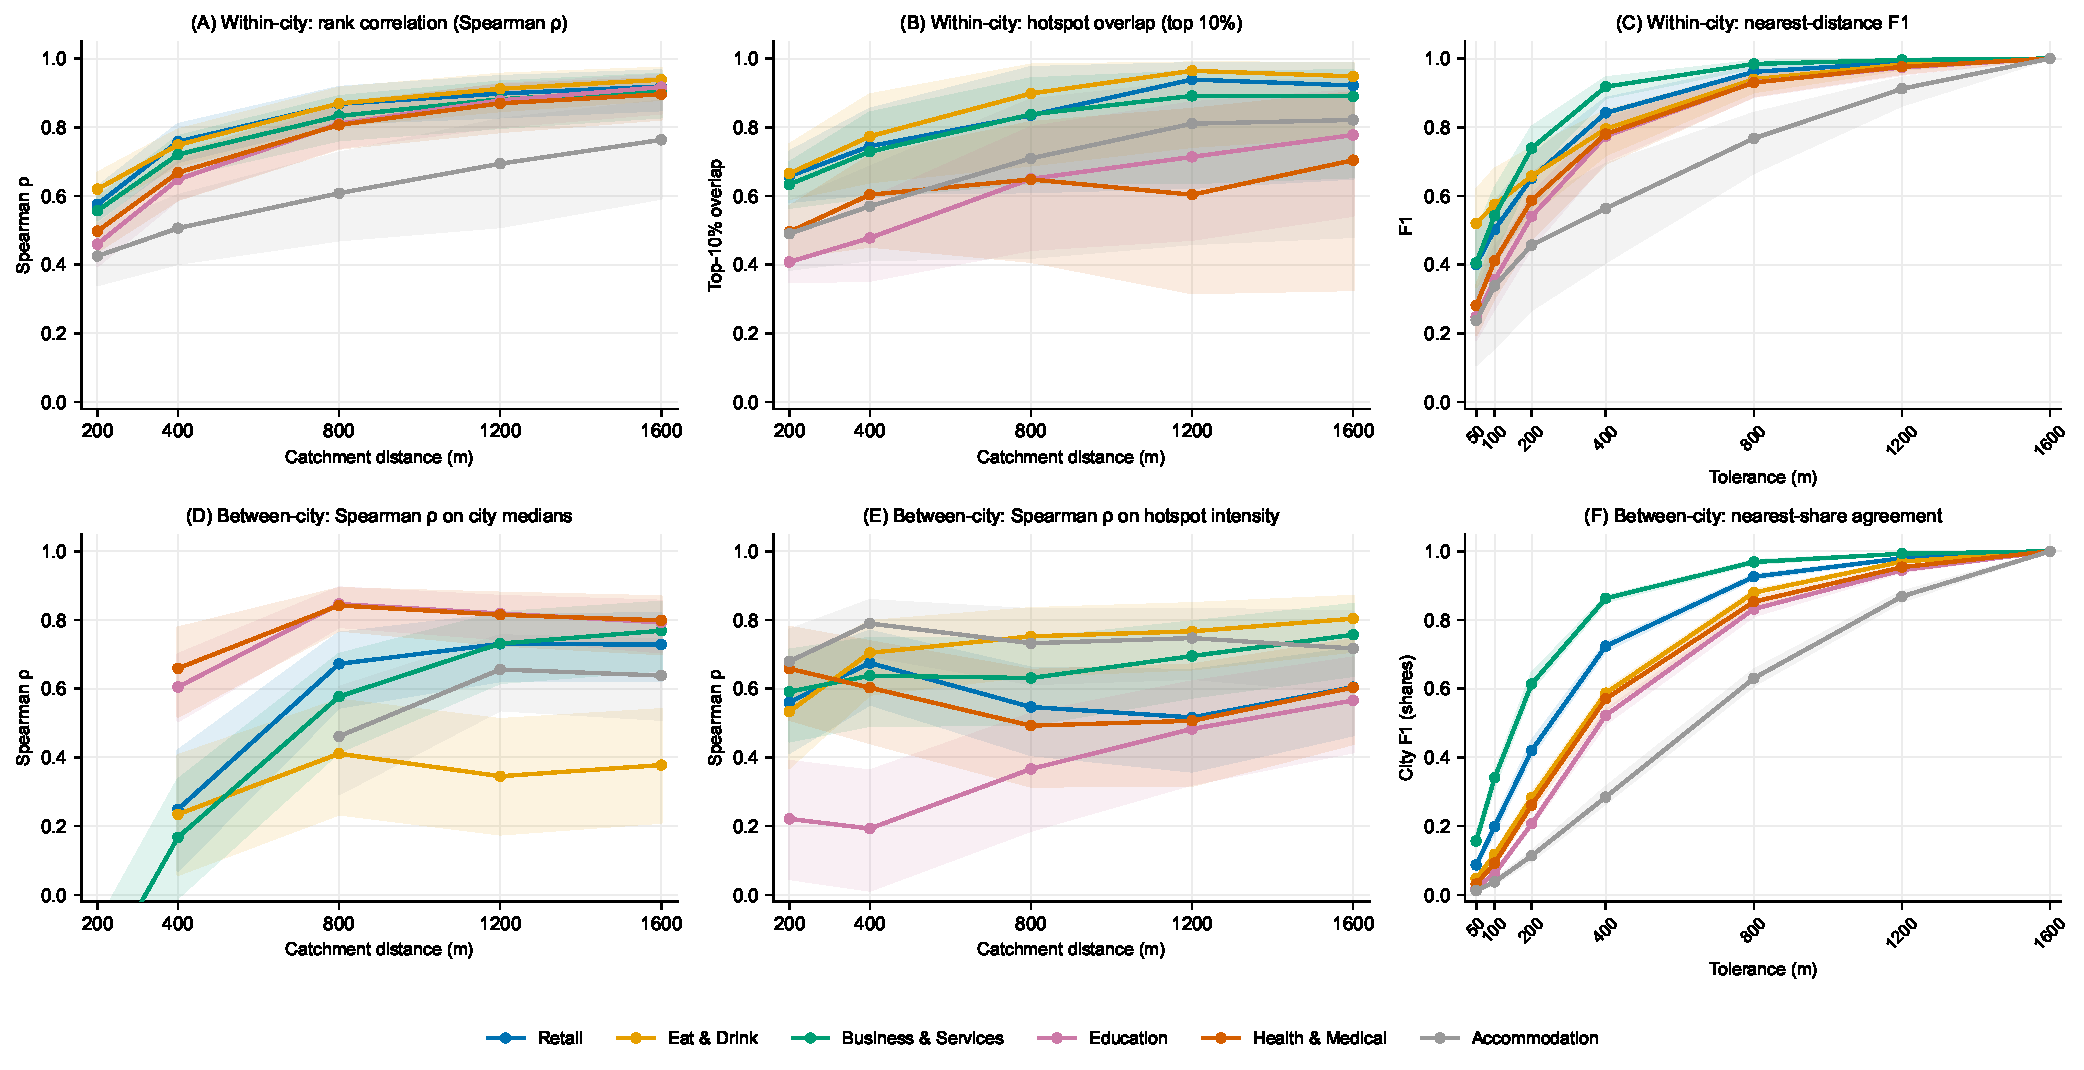
\includegraphics[width=\textwidth]{outputs/figures/fig_pointa_agreement_panels.pdf}
  \caption{\textbf{POI source-substitution agreement by category, task, and spatial scale.}
    \NRefCities{} reference cities. Top row (within-city): (A)~rank correlation (Spearman $\rho$), (B)~hotspot overlap, and (C)~nearest-within-tolerance F1; shaded bands show 95\% spatial block bootstrap CIs (distance-adaptive blocks, $B=200$). Bottom row (between-city): (D)~Spearman $\rho$ on city-level median counts, (E)~Spearman $\rho$ on city-level hotspot intensity, and (F)~harmonic-mean agreement of city-level nearest shares; shaded bands show 95\% city-level bootstrap CIs ($B=2{,}000$).
  }
  \label{fig:pointa_agreement_panels}
\end{figure}

\subsection{Per-city variability}
\label{sec:poi-supp-city-variability}

The main-text figures report median agreement across reference cities. Figure~\ref{fig:pointa_city_variability} shows the underlying per-city distributions at two representative catchment distances (400\,m and 800\,m). The strip plots confirm that the medians are not driven by a small number of outlier cities: at 800\,m most categories have tight distributions for rank correlation, with the bulk of cities exceeding 80\% concordance. Accommodation and Health \& Medical remain consistently the weakest categories with the widest spreads. Figure~\ref{fig:pointa_cross_city_scatter} complements this by plotting city-level median accessibility (log-transformed counts) from Overture against registry values at 800\,m; points falling below the identity line indicate systematic undercounting by Overture, particularly for Retail and Eat \& Drink.

\begin{figure}[p]
  \centering
  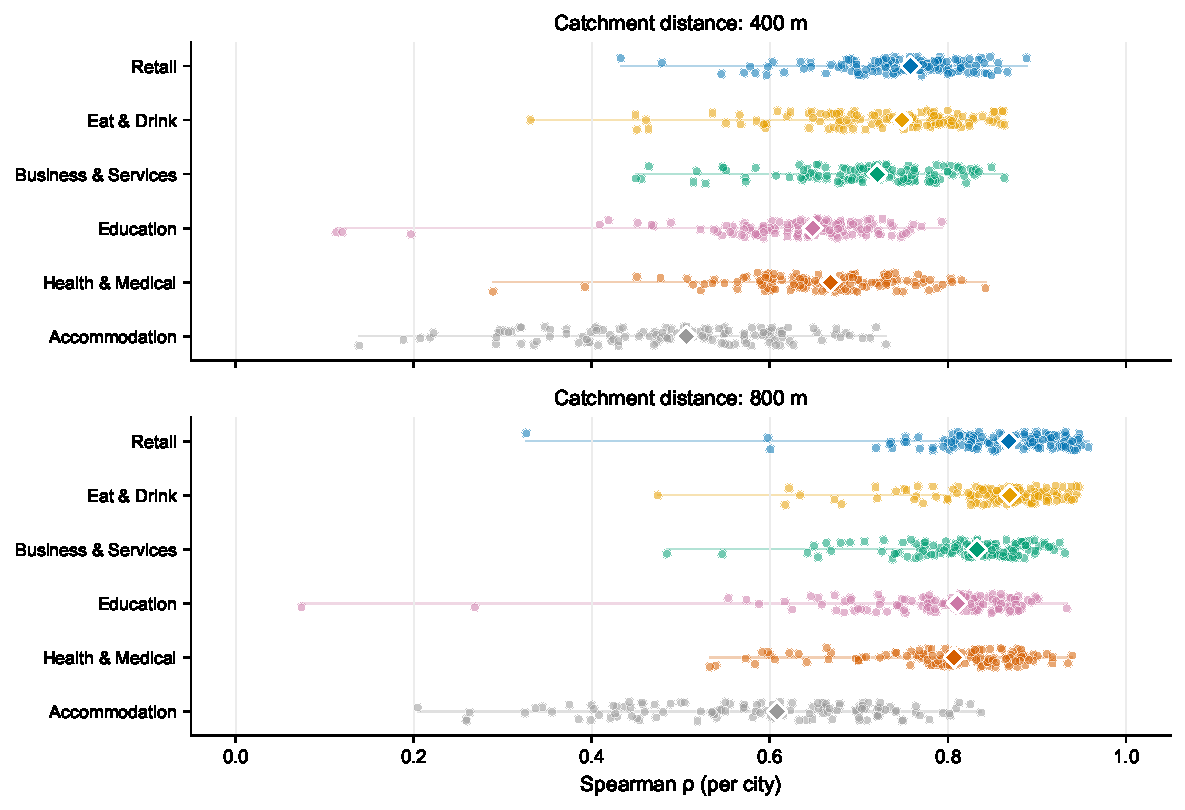
\includegraphics[width=0.88\textwidth]{outputs/figures/fig_pointa_city_variability.pdf}
  \caption{\textbf{Per-city rank correlation spread.}
    Distribution of Spearman $\rho$ (segment-level unweighted counts) across \NRefCities{} reference cities at 400\,m and 800\,m catchments. Points show individual cities; diamonds mark medians.
  }
  \label{fig:pointa_city_variability}

  \vspace{0.5em}

  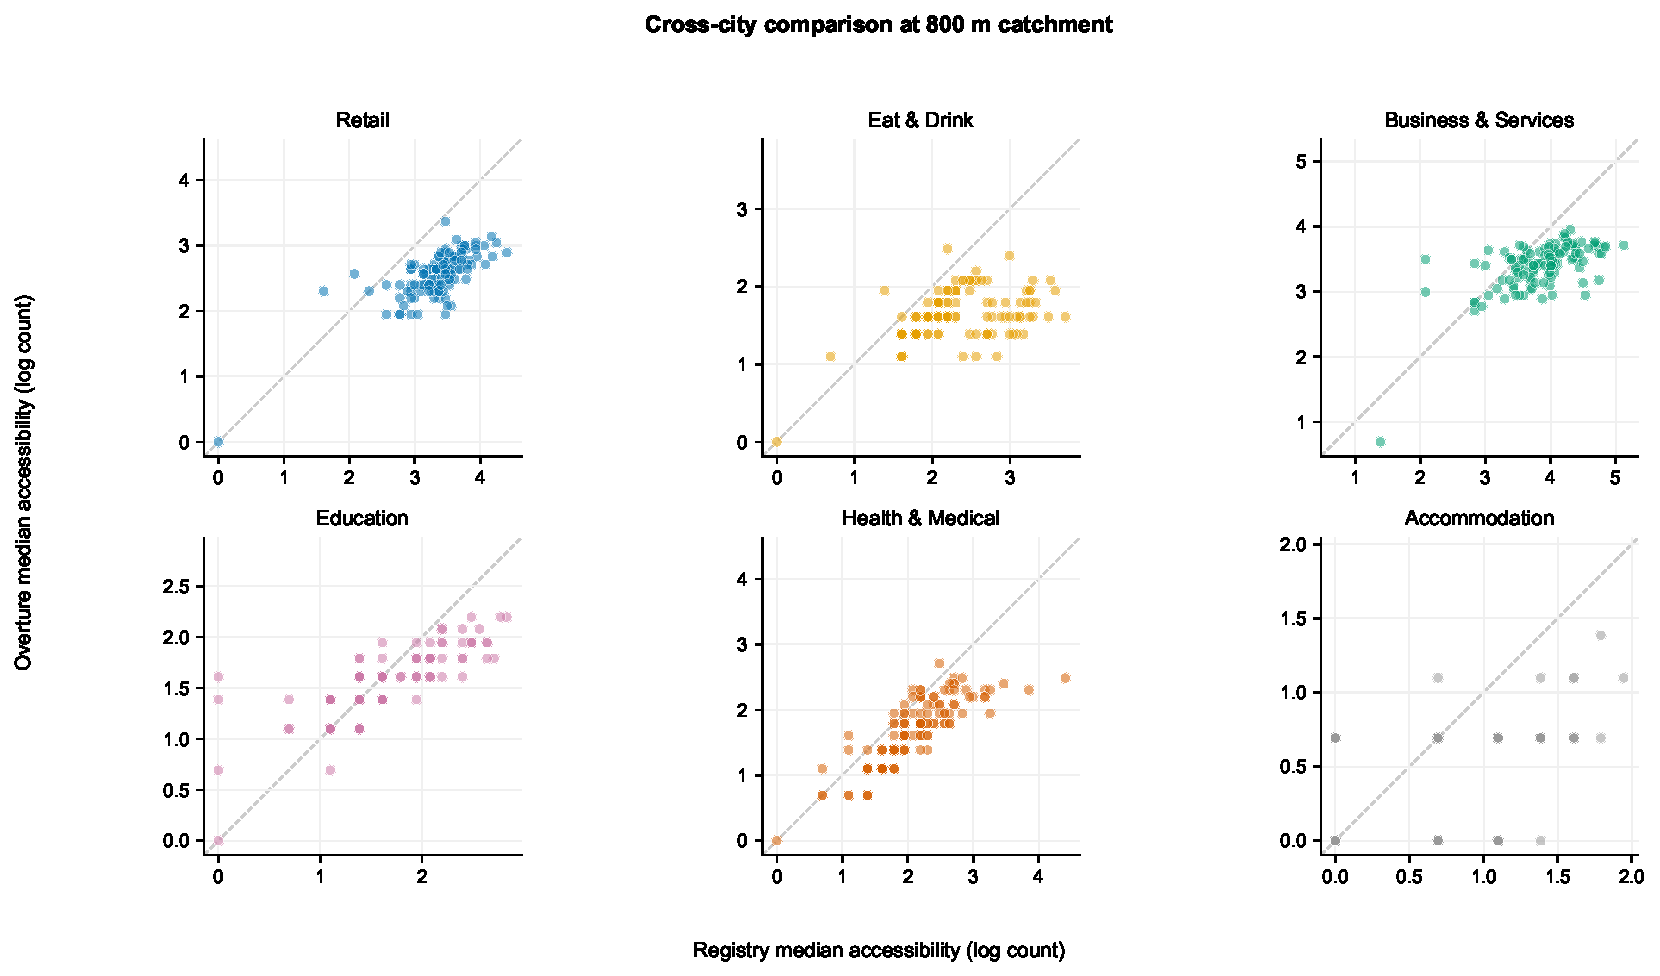
\includegraphics[width=0.88\textwidth]{outputs/figures/fig_pointa_cross_city_scatter.pdf}
  \captionof{figure}{\textbf{Cross-city comparison at 800\,m catchment.}
    Each point is one reference city. Axes show median log-transformed POI counts from registry and Overture sources; the dashed line marks identity. The predominance of points below the line indicates systematic undercounting by Overture, especially for Retail and Eat \& Drink.
  }
  \label{fig:pointa_cross_city_scatter}
\end{figure}

\subsection{Distance-weighted accessibility}
\label{sec:poi-supp-weighted}

The main-text results use unweighted POI counts (the number of establishments reachable within each catchment distance). An alternative is distance-weighted counts, where each POI's contribution decays with network distance, giving greater weight to nearer establishments.

At the same catchment distance, weighted counts produce lower concordance than unweighted counts (typically 3--5 percentage points for rank correlation, 5--8 for hotspot overlap), because the gravity weighting amplifies the effect of small geocoding offsets between sources. However, the weighted measure at 800\,m still exceeds the unweighted measure at 400\,m across all categories, since the larger catchment more than compensates for the concordance lost to weighting. This is relevant for applications that prefer distance-weighted accessibility: reliable concordance is achievable at 800\,m or above. The nearest-distance columns are unchanged, as they do not involve count aggregation.

\clearpage
\section{Building Footprint Source Composition and Metric Sensitivity}
\label{sec:bldg-supp}

This supplement documents the provenance composition of the Overture Maps building footprints used in SOAR-EU and quantifies its effect on derived morphometric indicators.

\subsection{Source classification}
\label{sec:bldg-supp-classification}

Each Overture building footprint carries a \texttt{sources} JSON array whose first element identifies the contributing dataset. We classify these into two groups: \emph{community-contributed} (OpenStreetMap, Esri Community Maps, national cadastral agencies) and \emph{ML-derived} (Microsoft ML Buildings, Google Open Buildings). Community-contributed footprints are digitised or imported from authoritative cadastral sources and generally preserve individual building boundaries; ML-derived footprints are segmented from satellite imagery and may merge adjacent buildings into single polygons or introduce unintended gaps between genuinely attached structures.

Across the \NCitiesTotal{} cities, the footprints draw on several source datasets: OpenStreetMap (dominant in most European cities), Esri Community Maps, Microsoft ML Buildings, and, in Spain, the Instituto Geogr\'{a}fico Nacional cadastre. Country-level aggregates reveal a clear geographic gradient (Table~\ref{tab:building_source_country}; Figure~\ref{fig:building_source_map}): the Netherlands, France, Switzerland, and Belgium are dominated by community sources, while Romania, Spain, Greece, and Bulgaria rely substantially on ML-derived footprints. The per-city ML fraction (Min and Max columns of Table~\ref{tab:building_source_country}) spans from zero in several cadastral-import cities to a large majority in the most ML-reliant. Per-city counts by dataset and country-level summaries are provided in the accompanying CSV files.

\begin{table}[!htb]
  \centering
  \caption{Building footprint source composition by country, sorted by ML-derived fraction (ascending). ML~(\%) is the proportion of footprints from ML-derived sources (primarily Microsoft ML Buildings); Min and Max show the per-city range within each country.}
  \label{tab:building_source_country}
  \scriptsize
  \begin{tabular}{@{}lrrrrr@{}}
  \toprule
  \textbf{Country} & \textbf{Cities} & \textbf{Buildings} & \textbf{ML (\%)} & \textbf{Min (\%)} & \textbf{Max (\%)} \\
  \midrule
  Netherlands & 43 & 6,209,242 & 1.6 & 0.0 & 20.6 \\
  Switzerland & 17 & 794,674 & 4.1 & 0.0 & 11.6 \\
  Luxembourg & 1 & 40,614 & 4.4 & 4.4 & 4.4 \\
  France & 73 & 10,245,743 & 4.5 & 0.0 & 15.2 \\
  Belgium & 16 & 2,627,084 & 5.2 & 1.0 & 16.2 \\
  Ireland & 5 & 769,998 & 5.4 & 3.3 & 8.4 \\
  Norway & 7 & 606,824 & 6.6 & 4.8 & 10.1 \\
  Finland & 6 & 367,553 & 7.8 & 6.2 & 13.5 \\
  Austria & 8 & 688,439 & 8.1 & 4.6 & 18.4 \\
  Denmark & 5 & 647,562 & 8.4 & 5.7 & 9.4 \\
  Estonia & 2 & 102,363 & 8.5 & 6.1 & 13.5 \\
  Germany & 99 & 11,601,375 & 8.8 & 0.1 & 35.7 \\
  Slovakia & 7 & 303,986 & 13.9 & 10.6 & 19.4 \\
  Slovenia & 2 & 98,624 & 15.3 & 13.4 & 19.0 \\
  Lithuania & 4 & 228,098 & 15.7 & 7.8 & 27.1 \\
  Latvia & 2 & 180,865 & 16.1 & 15.8 & 16.7 \\
  Czechia & 12 & 763,959 & 16.7 & 11.6 & 22.1 \\
  Italy & 88 & 4,246,128 & 17.4 & 3.0 & 81.0 \\
  Sweden & 17 & 793,793 & 18.5 & 0.7 & 50.7 \\
  Poland & 63 & 3,612,250 & 18.6 & 4.8 & 37.1 \\
  Croatia & 5 & 272,798 & 24.6 & 16.6 & 33.8 \\
  Hungary & 13 & 944,965 & 27.3 & 16.8 & 61.3 \\
  Portugal & 8 & 916,488 & 27.6 & 18.5 & 57.3 \\
  Bulgaria & 6 & 290,571 & 30.8 & 23.8 & 46.9 \\
  Greece & 8 & 871,146 & 31.3 & 7.5 & 94.9 \\
  Spain & 79 & 3,363,448 & 46.3 & 4.7 & 94.9 \\
  Romania & 29 & 1,319,339 & 48.0 & 23.6 & 86.1 \\
  Malta & 1 & 49,893 & 54.8 & 54.8 & 54.8 \\
  \bottomrule
\end{tabular}
\end{table}

\begin{figure}[!htb]
  \centering
  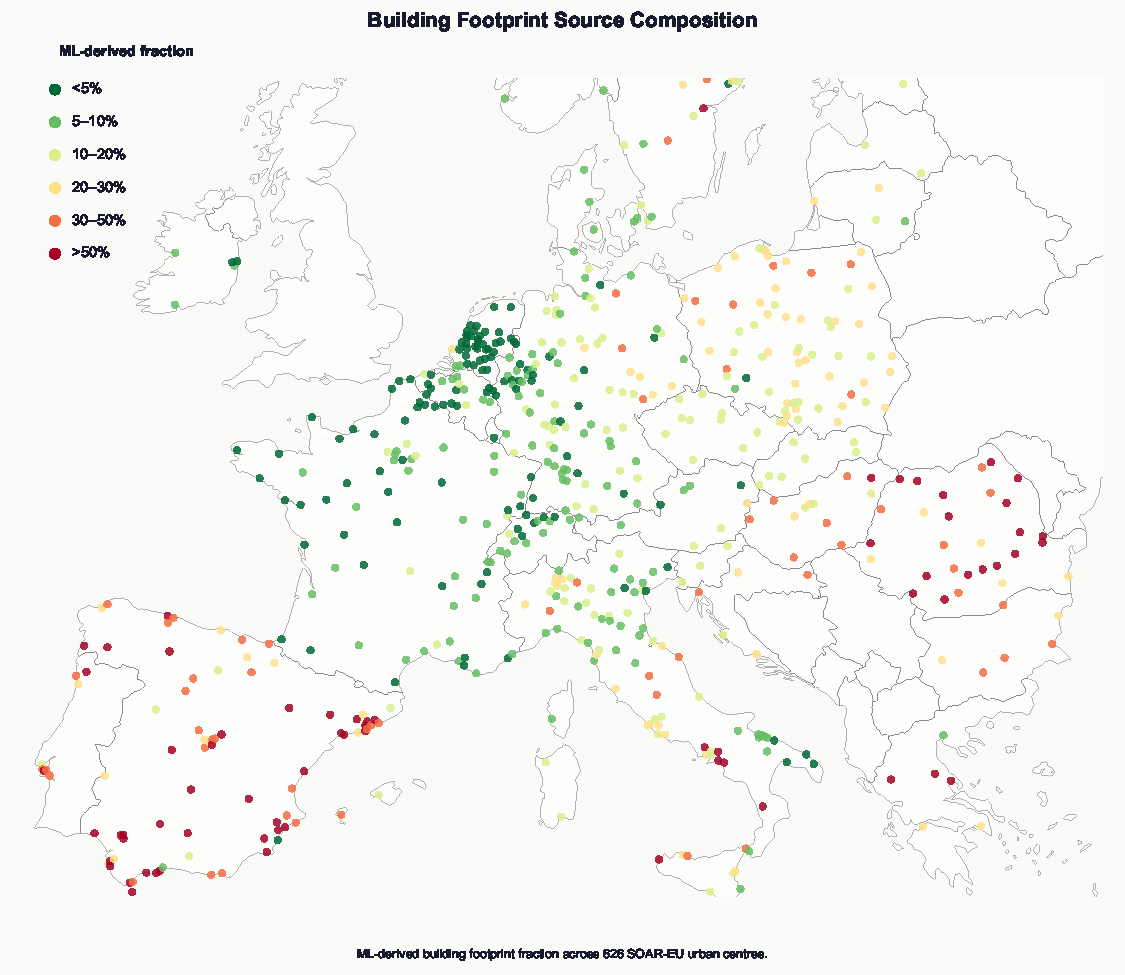
\includegraphics[width=\textwidth]{outputs/figures/fig_building_source_map.pdf}
  \caption{ML-derived building footprint fraction across the \NCitiesTotal{} SOAR-EU urban centres. Cities in western and northern Europe (France, Netherlands, Belgium, Germany) are dominated by community-contributed sources; cities in southern and eastern Europe (Romania, Spain, Greece, Bulgaria) rely more heavily on ML-derived footprints.}
  \label{fig:building_source_map}
\end{figure}

\subsection{Effect on morphometric indicators}
\label{sec:bldg-supp-sensitivity}

We test for source-driven bias at two levels.

\paragraph{Cross-city correlations.} For each morphometric indicator, we compute the Spearman correlation between each city's ML fraction and its median metric value across the \NCitiesTotal{} cities (Table~\ref{tab:building_metric_sensitivity}). Shared wall ratio shows the strongest negative association: cities with more ML-derived buildings have lower shared wall ratios. This cross-city correlation conflates two effects: a genuine morphological gradient (countries with higher ML fractions---Romania, Bulgaria, Greece---also have more freestanding housing stock) and a data artefact (ML-derived footprints underestimate shared walls due to polygon boundary gaps). The within-city test below isolates the artefact component. Perimeter, area, and volume are also positively associated, partly reflecting the tendency of ML segmentation to merge adjacent buildings into larger polygons and partly reflecting genuinely larger building footprints in lower-density settings. Fractal dimension and corner count show weaker but significant associations, while compactness, shape index, and orientation show no significant association with source composition.

\paragraph{Within-city comparisons.} To isolate the data artefact from genuine morphological differences between countries, we compare community and ML-derived buildings \emph{within the same city} using Mann-Whitney $U$ tests, restricted to cities containing both source types (Table~\ref{tab:building_metric_sensitivity}). Shared wall ratio shows a consistent within-city difference, significant in nearly all such cities: ML-derived buildings have lower shared wall ratios than community-contributed buildings in the same urban context, confirming a per-building artefact independent of cross-country morphological variation. Corner count and fractal dimension are also affected within cities, while compactness and shape index show small but widespread differences.

Block-level density metrics (GSI, FSI) show no meaningful cross-city association with ML fraction, likely because ML footprints add buildings in areas where community mapping is sparse, compensating for any area inflation from polygon merging. Table~\ref{tab:building_metric_sensitivity} summarises all cross-city and within-city results.

\begin{table}[!htb]
  \centering
  \caption{Sensitivity of building morphometric indicators to data source composition. Cross-city $\rho$: Spearman correlation between city ML fraction and city median metric value, across all \NCitiesTotal{} cities. Within-city $r$: median rank-biserial correlation from Mann-Whitney $U$ tests comparing community and ML-derived buildings within each city, restricted to cities containing both source types. Significance: {*}{*}{*}\,$p < 0.001$, {*}{*}\,$p < 0.01$, {*}\,$p < 0.05$.}
  \label{tab:building_metric_sensitivity}
  \scriptsize
  \begin{tabular}{@{}lrrrl@{}}
  \toprule
  \textbf{Metric} & \textbf{Cross-city $\rho$} & \textbf{$p$} & \textbf{Within-city $r$} & \textbf{Sig.} \\
  \midrule
  Perimeter & +0.534 & $<$0.001 & --- & *** \\
  Shared Wall Ratio & -0.515 & $<$0.001 & -0.36 & *** \\
  Area & +0.513 & $<$0.001 & --- & *** \\
  Volume & +0.508 & $<$0.001 & --- & *** \\
  Shared Walls & -0.437 & $<$0.001 & --- & *** \\
  Block FSI & +0.372 & $<$0.001 & --- & *** \\
  Form Factor & -0.217 & $<$0.001 & --- & *** \\
  Fractal Dimension & -0.196 & $<$0.001 & -0.12 & *** \\
  Frontage Max & -0.178 & $<$0.001 & --- & *** \\
  Block GSI & +0.111 & 0.006 & --- & ** \\
  Corners & +0.098 & 0.015 & -0.26 & * \\
  Mean Height & +0.098 & 0.016 & --- & * \\
  Orientation & -0.060 & 0.136 & --- &  \\
  Compactness & +0.055 & 0.171 & +0.13 &  \\
  Shape Index & +0.055 & 0.171 & +0.13 &  \\
  \bottomrule
\end{tabular}
\end{table}

\subsection{Street-frontage ratio}
\label{sec:bldg-supp-frontage}

To provide a source-robust continuity measure, we compute a bilateral street-frontage ratio for each street segment. The computation proceeds as follows: (1)~buffer the street centreline by 35\,m to define a corridor (wide enough to capture building edges that address the street across a typical European front-garden or setback depth, narrow enough to exclude buildings on the next parallel street); (2)~identify all building edges whose midpoint falls inside the corridor and whose nearest street is this one (preventing cross-street contamination); (3)~classify each edge as left or right of the centreline using the local street tangent; (4)~per side, retain only edges within 5\,m of the closest edge, filtering out rear extensions and garages while preserving the primary facade line (5\,m is chosen to span typical facade step-ins and arcades without admitting rear-yard structures); (5)~project retained edges onto the centreline, merge overlapping intervals, and compute coverage as the fraction of street length covered (3\,m trimmed from each end as a junction guard, removing the short overlap where a corner property's facade would otherwise count toward both intersecting streets); (6)~the reported score (\texttt{frontage\_max}) is the maximum of the two sides. Per-side scores (\texttt{frontage\_left}, \texttt{frontage\_right}), their mean (\texttt{frontage\_avg}), and per-side edge counts (\texttt{frontage\_edges\_left}, \texttt{frontage\_edges\_right}) are also retained.

Unlike shared wall ratio, which requires exact topological contact between adjacent polygon boundaries, frontage ratio depends only on building \emph{presence} along the street edge. Whether two adjacent terraced houses are represented as separate touching polygons (community-digitised) or as a single merged polygon (ML-derived), the frontage coverage is the same. Across the \NCitiesTotal{} cities, the association between city-level ML fraction and median frontage ratio is substantially weaker than the corresponding shared-wall-ratio association (Table~\ref{tab:building_metric_sensitivity}). Because frontage is largely immune to the polygon-merging artefact that the within-city test identifies for shared wall ratio, this weaker residual association most likely reflects a predominantly genuine morphological gradient (countries with higher ML fractions also tend toward more freestanding housing) rather than a measurement artefact.

\end{document}
'
%
% If you hit a cryptic build error after edits (e.g., "Runaway argument" while
% writing labels/outlines), remove auxiliary files and rebuild:
%   rm -f manuscript.aux manuscript.out manuscript.toc manuscript.bbl manuscript.blg
%   pdflatex manuscript.tex && pdflatex manuscript.tex
\providecommand{\preprintmode}{0}
\newcommand{\IfPreprintTF}[2]{\ifnum\preprintmode=1\relax #1\else #2\fi}
\newcommand{\SpecsTableHeading}{\IfPreprintTF{Dataset summary}{Specifications Table}}
\newcommand{\ValueHeading}{\IfPreprintTF{Value of the dataset}{Value of the Data}}

% Submission placeholders (override at build time if desired)
\providecommand{\ZenodoDoi}{10.5281/zenodo.18961227}
\providecommand{\ZenodoUrl}{https://doi.org/10.5281/zenodo.18961227}
\providecommand{\GrantNumber}{101078890}

\usepackage[utf8]{inputenc}
\usepackage[margin=2.5cm]{geometry}
\usepackage{graphicx}
\usepackage{booktabs}
\PassOptionsToPackage{hyphens}{url}\usepackage{hyperref}
\usepackage{siunitx}
\usepackage{xcolor}
\usepackage{longtable}
\usepackage{multirow}
\usepackage{array}
\usepackage{float}        % Better float positioning
\usepackage{placeins}     % \FloatBarrier command
\usepackage{enumitem}     % Better list formatting
\usepackage{caption}      % \captionof for multi-figure floats
\usepackage{wrapfig}      % text-wrapping figures
\usepackage{amssymb}      % For \checkmark symbol
\usepackage{pdflscape}    % For landscape pages in supplementary

% Avoid hyperref warnings from elsarticle author-note macros in PDF strings
% (e.g., when writing metadata/bookmarks).
\makeatletter
\pdfstringdefDisableCommands{%
  \def\corref#1{}%
  \def\cnotenum{}%
  \def\@corref#1{}%
}
\makeatother

% Allow line breaks after underscores so long \texttt{} filenames
% (e.g. building\_source\_counts.csv) can wrap instead of overrunning the margin.
\renewcommand{\_}{\textunderscore\allowbreak}

% Auto-generated statistics macros (from paper_stats.json)
% Auto-generated LaTeX macros
% Generated by: python paper_data/code/s06_write_paper_macros.py
% DO NOT EDIT MANUALLY - regenerate from source data
% === City Counts ===
\newcommand{\NCitiesTotal}{626}
\newcommand{\NCountries}{28}
\newcommand{\NRefCities}{116}
\newcommand{\NRefCitiesFr}{73}
\newcommand{\NRefCitiesNl}{43}
\newcommand{\NNonRefCities}{510}

% === Data Coverage ===
\newcommand{\NCitiesLowHeight}{94}
\newcommand{\NCitiesNoHeight}{20}
\newcommand{\NCitiesWithHeightsRaster}{611}
\newcommand{\BldgHeightsAgeYears}{14}
\newcommand{\MedianHeightCoverage}{71}
\newcommand{\MedianBlockHundredCoverage}{74}
\newcommand{\NCitiesNoBlocks}{24}
\newcommand{\NCitiesNoEmployment}{185}

% === Dataset Size ===
\newcommand{\DatasetTotalCompressedGB}{35}
\newcommand{\DatasetMinMB}{3.5}
\newcommand{\DatasetMaxGB}{1.2}
\newcommand{\DatasetMeanMB}{56}

% === POI Validation Thresholds ===
\newcommand{\PoiNearDistGoodM}{800}
\newcommand{\PoiNearDistOtherM}{800}
\newcommand{\PoiNearDistAccomM}{1200}

% === Displacement Stats ===


% Consistent table column types
\newcolumntype{L}[1]{>{\raggedright\arraybackslash}p{#1}}
\newcolumntype{C}[1]{>{\centering\arraybackslash}p{#1}}
\newcolumntype{R}[1]{>{\raggedleft\arraybackslash}p{#1}}

\IfPreprintTF{}{\journal{Data in Brief}}

\begin{document}

\begin{frontmatter}

  \title{SOAR-EU: A Scalable, Open, Automatable, and Reproducible European Urban Dataset}

  \author[spacesyntax]{Gareth Simons\corref{cor1}}
  \ead{gareth.simons@ucl.ac.uk}
  \cortext[cor1]{Corresponding author}

  \author[spacesyntax]{Kayvan Karimi}
  \author[spacesyntax]{Sepehr Zhand}

  \affiliation[spacesyntax]{organization={Space Syntax Laboratory, UCL Bartlett School of Architecture},
    addressline={22 Gordon Street},
    city={London},
    country={United Kingdom}
  }

  \begin{abstract}
    Constructing spatial analytic datasets, particularly at scale, remains resource-intensive; SOAR-EU (Scalable, Open, Automatable, Reproducible --- European Urban) addresses this by providing ready-to-use pedestrian-scale urban metrics for \NCitiesTotal{} European cities across \NCountries{} countries to support comparative urban analytic research at the continental scale. Integrating GHS-UCDB urban boundaries, Eurostat census data, Copernicus Urban Atlas, and Overture Maps, it delivers over 100 pre-computed metrics per street at multiple spatial scales, covering network centrality, land-use and infrastructure accessibility, mixed-use diversity, building and block morphology, green-space and tree-canopy proximity, and demographics. Processing is automatable via open-source Python with fixed parameters; data are distributed as GeoPackage files in EPSG:3035. Because the Overture Maps POI layer aggregates commercial and editorial sources of varying completeness, we evaluate POI-derived accessibility through source-substitution replication against independent registries in \NRefCities{} reference cities in France and the Netherlands, providing task- and scale-specific guidance on when these metrics are more or less suitable for within-city pattern analysis and for broad between-city comparison.
  \end{abstract}

  \begin{keyword}
    pedestrian accessibility \sep
    street networks \sep
    land-use diversity \sep
    building morphology \sep
    walkability \sep
    cross-city comparison \sep
    spatial metrics
  \end{keyword}

\end{frontmatter}

%% ============================================================================
%% SPECIFICATIONS TABLE
%% ============================================================================
\section*{\SpecsTableHeading}

\begin{table}[!htbp]
  \centering
  \small
  \begin{tabular}{@{}L{3.2cm}L{8.3cm}@{}}
    \toprule
    \textbf{Subject} & Geography, Urban Studies, Geospatial Data Science \\
    \midrule
    \textbf{Specific subject area} & Urban morphology, pedestrian accessibility, land-use diversity \\
    \midrule
    \textbf{Type of data} & Table (geospatial vector); Processed, filtered (GeoPackage format) \\
    \midrule
    \textbf{Data format} & GeoPackage (.gpkg); one ZIP archive per country bundling the city GeoPackages, plus a boundary index file \\
    \midrule
    \textbf{How data was acquired} & Programmatic extraction and processing of open geospatial sources using Python (cityseer, momepy, GeoPandas). Metrics computed on natural street segments at multiple distance thresholds \\
    \midrule
    \textbf{Data collection} & Derived from publicly available authoritative sources: GHS-UCDB R2024A (2025 reference epoch), Overture Maps Foundation (2026 release), Copernicus Urban Atlas (2021), Copernicus Street Tree Layer (2021), Copernicus Height Model (2012), Eurostat Census Grid (2021) \\
    \midrule
    \textbf{Parameters for data collection} & Centrality thresholds: 400--9,600\,m. Accessibility thresholds: 200--1,600\,m. Morphology thresholds: 200--400\,m. CRS: EPSG:3035. See \href{https://github.com/UCL/t2e-soar-eu}{repository} for full configuration \\
    \midrule
    \textbf{Data source location} & Pan-European: \NCitiesTotal{} urban centres across 26 EU member states plus Norway and Switzerland (Liechtenstein has no qualifying urban centre under the GHS-UCDB threshold, and Cyprus is not covered by the GHS-UCDB R2024A European regional file used here). Coordinate Reference System: EPSG:3035 (ETRS89-LAEA Europe) \\
    \midrule
    \textbf{Data accessibility} & Repository: Zenodo. Data identification number: \ZenodoDoi{}. URL: \ZenodoUrl{} \\
    \midrule
    \textbf{Related research article} & G.\ Simons, K.\ Karimi, S.\ Zhand, A Morphological Atlas of European Urbanism: Eight Types of Urban Fabric Across Six Hundred Cities (SOAR-EU), submitted to \textit{Computers, Environment and Urban Systems}. \\
    \bottomrule
  \end{tabular}
\end{table}

%% ============================================================================
%% VALUE OF THE DATA
%% ============================================================================
\section*{\ValueHeading}

\begin{itemize}[leftmargin=*]
  \item The dataset enables \textbf{consistent comparative research} by removing the methodological confounds that usually frustrate cross-city work: all \NCitiesTotal{} cities are processed with identical methods, parameters, and source datasets, so measured differences reflect the urban fabric rather than differing analytical choices or bespoke data pipelines. This shared baseline supports benchmarking against continental norms, clustering streets into urban typologies, and detecting systematic differences in walkability and land use. Comparability is nonetheless bounded by the geographic consistency of the underlying open sources (Section~\ref{sec:provenance}): broad distributional comparison across regions and city groups is more strongly supported than exact city-by-city ranking, particularly for POI-derived metrics outside the validated French and Dutch reference set.
  \item The \textbf{multi-scale design} supports sensitivity analysis and scale-appropriate interpretation. Centrality metrics span 400\,m to 9,600\,m (5--120 minute walking catchments); accessibility metrics span 200\,m to 1,600\,m. Because relationships observed at one scale may not hold at others \cite{openshaw1984}, multiple thresholds are provided.
  \item The dataset supports \textbf{network-based accessibility} analysis that follows pedestrian routes rather than Euclidean buffers \cite{apparicio2008}. A park 200\,m as-the-crow-flies but 800\,m by foot is treated as 800\,m away. For each land-use category, both unweighted and distance-weighted counts are provided, supporting more nuanced aggregations in which proximity can be weighted by distance impedance.
  \item Researchers can benefit from the \textbf{fine-grained resolution} at street-segment level, which preserves within-neighbourhood heterogeneity and supports analysis from individual streets to city-wide patterns.
  \item The pipeline supports \textbf{reproducibility}: processing code and parameter settings are documented, enabling researchers to verify, regenerate, or extend the dataset as sources improve.
  \item The dataset benefits \textbf{urban planners, transport researchers, public health scientists, and environmental analysts} who need comparable pedestrian-scale indicators across European cities but lack the resources to assemble multi-source geospatial pipelines from scratch.
\end{itemize}

%% ============================================================================
%% OBJECTIVE
%% ============================================================================
\section*{Objective}

Comparative urban research requires consistent measurement across cities, yet constructing spatial analytic datasets remains resource-intensive. Related work includes GHSL \cite{pesaresi2023} global built-up surface mapping, Boeing's \cite{boeing2020} analysis of US street networks, Fleischmann et al.'s \cite{fleischmann2022} numerical taxonomy of urban form, and Yap and Biljecki's \cite{yap2023} feature-rich network dataset for 50 cities. Simons's \cite{simons2021thesis} pedestrian-scale integration of street networks, land use, and census demographics across 931 cities and towns in Great Britain is a direct methodological precursor to the present continental-scale dataset.

SOAR-EU (Scalable, Open, Automatable, Reproducible --- European Urban) complements these by providing ready-to-use pedestrian-scale metrics for \NCitiesTotal{} EU urban centres. The dataset integrates GHS-UCDB boundaries, Eurostat census grids, Copernicus land cover and building heights, and Overture Maps street networks and POIs. Metrics are computed on street segments across multiple spatial scales (200--9,600\,m) using the cityseer \cite{simons2023} Python package, spanning network centrality, land-use and infrastructure accessibility, mixed-use diversity, building and block morphology, green-space and tree-canopy proximity, and demographics. The pipeline is open-source and designed for regeneration as future data releases become available.

%% ============================================================================
%% DATA DESCRIPTION
%% ============================================================================
\section{Data Description}

\subsection{Dataset Structure}
\label{sec:dataset-structure}

The dataset comprises a \texttt{boundaries.gpkg} file derived from the GHS-UCDB urban centre boundaries, plus \NCountries{} country-level ZIP archives (\texttt{soar\_eu\_\{country\}.zip}) that bundle the \NCitiesTotal{} individually compressed city GeoPackages. Each city file follows the naming convention \texttt{metrics\_\{bounds\_fid\}.gpkg.zip}, where \texttt{bounds\_fid} corresponds to the unique identifier from \texttt{boundaries.gpkg}.

Each GeoPackage contains three layers: \textbf{streets} (natural street segments with computed metrics as LineString geometries), \textbf{buildings} (individual footprints with morphological attributes), and \textbf{blocks} (urban blocks with source and morphological attributes). The streets layer contains only \emph{live} segments (those whose midpoint falls within the urban centre boundary), excluding peripheral buffer segments used solely for edge-effect mitigation during network and accessibility analysis. Individual city files range from approximately \DatasetMinMB\,MB to \DatasetMaxGB\,GB depending on urban extent (average $\sim$\DatasetMeanMB\,MB); the complete compressed dataset is approximately \DatasetTotalCompressedGB\,GB. End-to-end processing takes approximately one day on a contemporary workstation-class laptop (18-core Apple M5 Pro).

Per-column completeness and building-source composition tables (\texttt{completeness\_coverage.csv}, \texttt{building\_source\_counts.csv}, and \texttt{building\_source\_by\_country.csv}) are bundled with the deposit; coverage is summarised in Section~\ref{sec:coverage} and source composition is interpreted in Section~\ref{sec:provenance}.

\subsection{Streets Layer}

The streets layer is the core of the dataset: each live segment carries pre-computed metrics spanning the full set of measure families: network centrality, land-use accessibility and mixed-use diversity, infrastructure accessibility, building and block morphology, green-space and tree-canopy proximity, and interpolated census demographics. Most are computed at several network-distance thresholds, indicated by a suffix (e.g., \texttt{\_400}, \texttt{\_800}). Table~\ref{tab:streets_schema} summarises the attribute groups; the complete per-column schema is given in Supplementary Material (Section~S1).

\begin{table}[!htbp]
  \centering
  \caption{Summary of streets layer attributes (selected metrics shown; full schema in Supplementary Material Section~S1).}
  \label{tab:streets_schema}
  \small
  \begin{tabular}{@{}L{4cm}L{8.1cm}@{}}
    \toprule
    \textbf{Attribute group} & \textbf{Description} \\
    \midrule
    \texttt{geometry}, \texttt{x}, \texttt{y} & Segment geometry and midpoint coordinates (EPSG:3035) \\
    \midrule
    \texttt{cc\_beta\_*} & Closeness centrality (gravity-weighted) at distance thresholds \\
    \midrule
    \texttt{cc\_harmonic\_*} & Harmonic closeness centrality \\
    \midrule
    \texttt{cc\_hillier\_*} & Hillier-type closeness (node count / mean distance) \\
    \midrule
    \texttt{cc\_farness\_*} & Farness (total network distance to reachable segments) \\
    \midrule
    \texttt{cc\_betweenness\_*} & Segment betweenness centrality \\
    \midrule
    \texttt{cc\_betweenness\_beta\_*} & Beta-weighted betweenness centrality \\
    \midrule
    \texttt{cc\_density\_*} & Street segment density within threshold \\
    \midrule
    \texttt{cc\_cycles\_*} & Network cycle count within threshold \\
    \midrule
    \texttt{cc\_\{landuse\}\_*\_nw} & Unweighted POI count for land-use category \\
    \midrule
    \texttt{cc\_\{landuse\}\_*\_wt} & Distance-weighted POI count for land-use category \\
    \midrule
    \texttt{cc\_\{landuse\}\_nearest\_max\_*} & Distance to nearest POI in category \\
    \midrule
    \texttt{cc\_\{infra\}\_*\_nw/wt} & Infrastructure accessibility: transport, parking, street-furniture counts \\
    \midrule
    \texttt{cc\_hill\_*} & Land-use diversity (Hill numbers $q=0,1,2$) \\
    \midrule
    \texttt{cc\_green\_nearest\_max\_*} & Distance to nearest green space \\
    \midrule
    \texttt{cc\_trees\_nearest\_max\_*} & Distance to nearest tree canopy \\
    \midrule
    \texttt{cc\_green\_area\_sum\_*}, \texttt{cc\_trees\_area\_sum\_*} & Green-space / tree-canopy area within threshold \\
    \midrule
    \texttt{cc\_*\_median\_*} & Building morphology, contextual aggregation (area, height, volume, compactness, shared-wall ratio, \ldots) \\
    \midrule
    \texttt{cc\_building\_*} & Building count within threshold \\
    \midrule
    \texttt{frontage\_max} & Bilateral street-frontage ratio: max(left, right) building coverage (0--1) \\
    \midrule
    \texttt{cc\_block\_*} & Contextual block morphology: area, perimeter, compactness, GSI, FSI, OSR, storeys, height \\
    \midrule
    \texttt{density}, \texttt{t}, \texttt{emp} & Interpolated census demographics (population, density, age, employment, nationality, migration) \\
    \bottomrule
  \end{tabular}
\end{table}

Two of these families, land-use and infrastructure accessibility, count points of interest grouped into analytical categories. The 11 land-use categories (\texttt{cc\_\{landuse\}\_*}) are listed in Table~\ref{tab:landuse} and the three infrastructure categories (\texttt{cc\_\{infra\}\_*}) in Table~\ref{tab:infrastructure}; both derive from Overture's classification as described in Section~\ref{sec:landuse-access}.

\begin{table}[!htbp]
  \centering
  \caption{Aggregated land-use categories derived from Overture Maps POI classification.}
  \label{tab:landuse}
  \small
  \begin{tabular}{@{}L{4.2cm}L{7.8cm}@{}}
    \toprule
    \textbf{Category} & \textbf{Includes} \\
    \midrule
    \texttt{eat\_and\_drink} & Restaurants, cafés, bars \\
    \texttt{retail} & Shops, supermarkets, pharmacies \\
    \texttt{business\_and\_services} & Automotive, beauty/spa, financial, home, professional services, real estate, travel agencies, pets, media, corporate offices \\
    \texttt{public\_services} & Government offices, libraries, civic facilities \\
    \texttt{health\_and\_medical} & Hospitals, doctors, dentists, optometrists \\
    \texttt{education} & Schools, universities, driving schools \\
    \texttt{accommodation} & Hotels, hostels, lodging \\
    \texttt{active\_life} & Sports facilities, fitness centres, recreation \\
    \texttt{arts\_and\_entertainment} & Cinemas, theatres, performance venues \\
    \texttt{attractions\_and\_activities} & Museums, landmarks, tourist attractions \\
    \texttt{religious} & Places of worship \\
    \bottomrule
  \end{tabular}
\end{table}

\begin{table}[!htbp]
  \centering
  \caption{Infrastructure categories derived from Overture Maps infrastructure theme.}
  \label{tab:infrastructure}
  \small
  \begin{tabular}{@{}L{3cm}L{9cm}@{}}
    \toprule
    \textbf{Category} & \textbf{Includes} \\
    \midrule
    \texttt{transport} & Bus stops, bus stations, railway stations, subway stations, ferry terminals, airports (including regional, international, seaplane), aerialway stations, helipads \\
    \texttt{street\_furn} & Benches, drinking water points, fountains, planters, plants, post boxes, picnic tables \\
    \texttt{parking} & Parking lots, motorcycle parking \\
    \bottomrule
  \end{tabular}
\end{table}

\subsection{Buildings and Blocks Layers}

The buildings layer contains individual building footprints derived from Overture Maps with morphological metrics including area, perimeter, compactness, orientation, estimated height (sampled from raster), volume, floor area, form factor, corners, shape index, shared wall ratio, and fractal dimension. Each footprint retains its Overture \texttt{sources} attribute, recording the contributing dataset (e.g., OpenStreetMap, Microsoft ML Buildings). The blocks layer provides urban block geometries derived from Urban Atlas with block-level morphology (area, perimeter, compactness, orientation, computed via the momepy package \cite{fleischmann2019}) and Spacematrix indicators: ground space index (GSI, building coverage ratio), floor space index (FSI), open space ratio (OSR), mean number of storeys (L), and area-weighted mean building height. Block-level morphology is reported only for built-up blocks; very small and oversized blocks are filtered out (appearing as NaN), with the thresholds and rationale given in Section~\ref{sec:metric-computation}.

\subsection{Coverage and Completeness}
\label{sec:coverage}

A per-column completeness report (\texttt{completeness\_coverage.csv}) is included with the dataset, listing the non-null coverage share for every attribute column in each city's streets, buildings, and blocks layers. Building footprint source composition is documented in \texttt{building\_source\_counts.csv} (per-city counts by source dataset) and \texttt{building\_source\_by\_country.csv} (country-level summaries); see Section~\ref{sec:provenance} for interpretation. Most metric groups (centrality, land-use and infrastructure accessibility, diversity, green-space and tree-canopy proximity, and building morphology) have near-complete coverage across all cities. Three categories exhibit variable coverage:

\begin{itemize}[nosep]
  \item \textbf{Height-derived metrics.} Building heights are sampled from the 2012 Copernicus Digital Height Model raster, whose spatial footprint does not cover all cities uniformly. Height-dependent attributes (mean height, volume, form factor, and their street-level contextual summaries) have a median coverage of \MedianHeightCoverage\%, with \NCitiesLowHeight{} cities below 50\% and \NCitiesNoHeight{} cities with no height data at all.\footnote{The \NCitiesNoHeight{}-city figure is derived per-column from \texttt{completeness\_coverage.csv}; it differs from the count of cities for which a Copernicus DHM raster was delivered at all (\NCitiesWithHeightsRaster{}/\NCitiesTotal{}) because some delivered rasters contain no usable pixels inside the city extent.}
  \item \textbf{Block morphology at 200\,m.} Contextual block metrics at the 200\,m threshold (area, perimeter, compactness, orientation, coverage ratio, and Spacematrix indicators) have a median coverage of \MedianBlockHundredCoverage\% (\NCitiesNoBlocks{} cities at zero). Coverage is reported over the filtered \emph{built-up} blocks layer that ships with each city file. Urban Atlas blocks classed as roads, rail, water, wetlands, agriculture, forest, green urban areas, sports/leisure, or otherwise exceeding 2\,km\textsuperscript{2} are excluded from urban morphological metrics (see Section~\ref{sec:metric-computation}), which particularly affects streets near city peripheries. The residual variability reflects a spatial scale effect: some street segments do not have any qualifying block within a 200\,m network radius. The same metrics at the 400\,m threshold have substantially higher coverage.
  \item \textbf{Employment.} Eurostat employment counts (\texttt{emp}, \texttt{emp\_\%}) are unavailable for \NCitiesNoEmployment{} cities, reflecting gaps in the upstream Census Grid. All other demographic variables (population, age structure, gender, nationality, migration) are near-universal.
\end{itemize}

\noindent The coverage report documents per-column coverage for each of these metric groups.

\subsection{Example Output}

Figure~\ref{fig:example-amsterdam} illustrates SOAR-EU output for Amsterdam, showing four representative metrics computed on the street network. Panel (A) shows closeness centrality at 800\,m, capturing network accessibility. Panel (B) shows retail catchment, the count of retail POIs reachable within 400\,m network distance, with higher values concentrated in the historic centre. Panel (C) shows distance to nearest green or blue space, indicating park and water proximity across the urban fabric. Panel (D) shows population density interpolated from the Eurostat Census Grid 2021 (1\,km\textsuperscript{2} resolution), expressed as persons per km\textsuperscript{2} of land surface. All metrics use network-based distances for aggregation, except for census statistics which are interpolated.

\begin{figure}[!htbp]
  \centering
  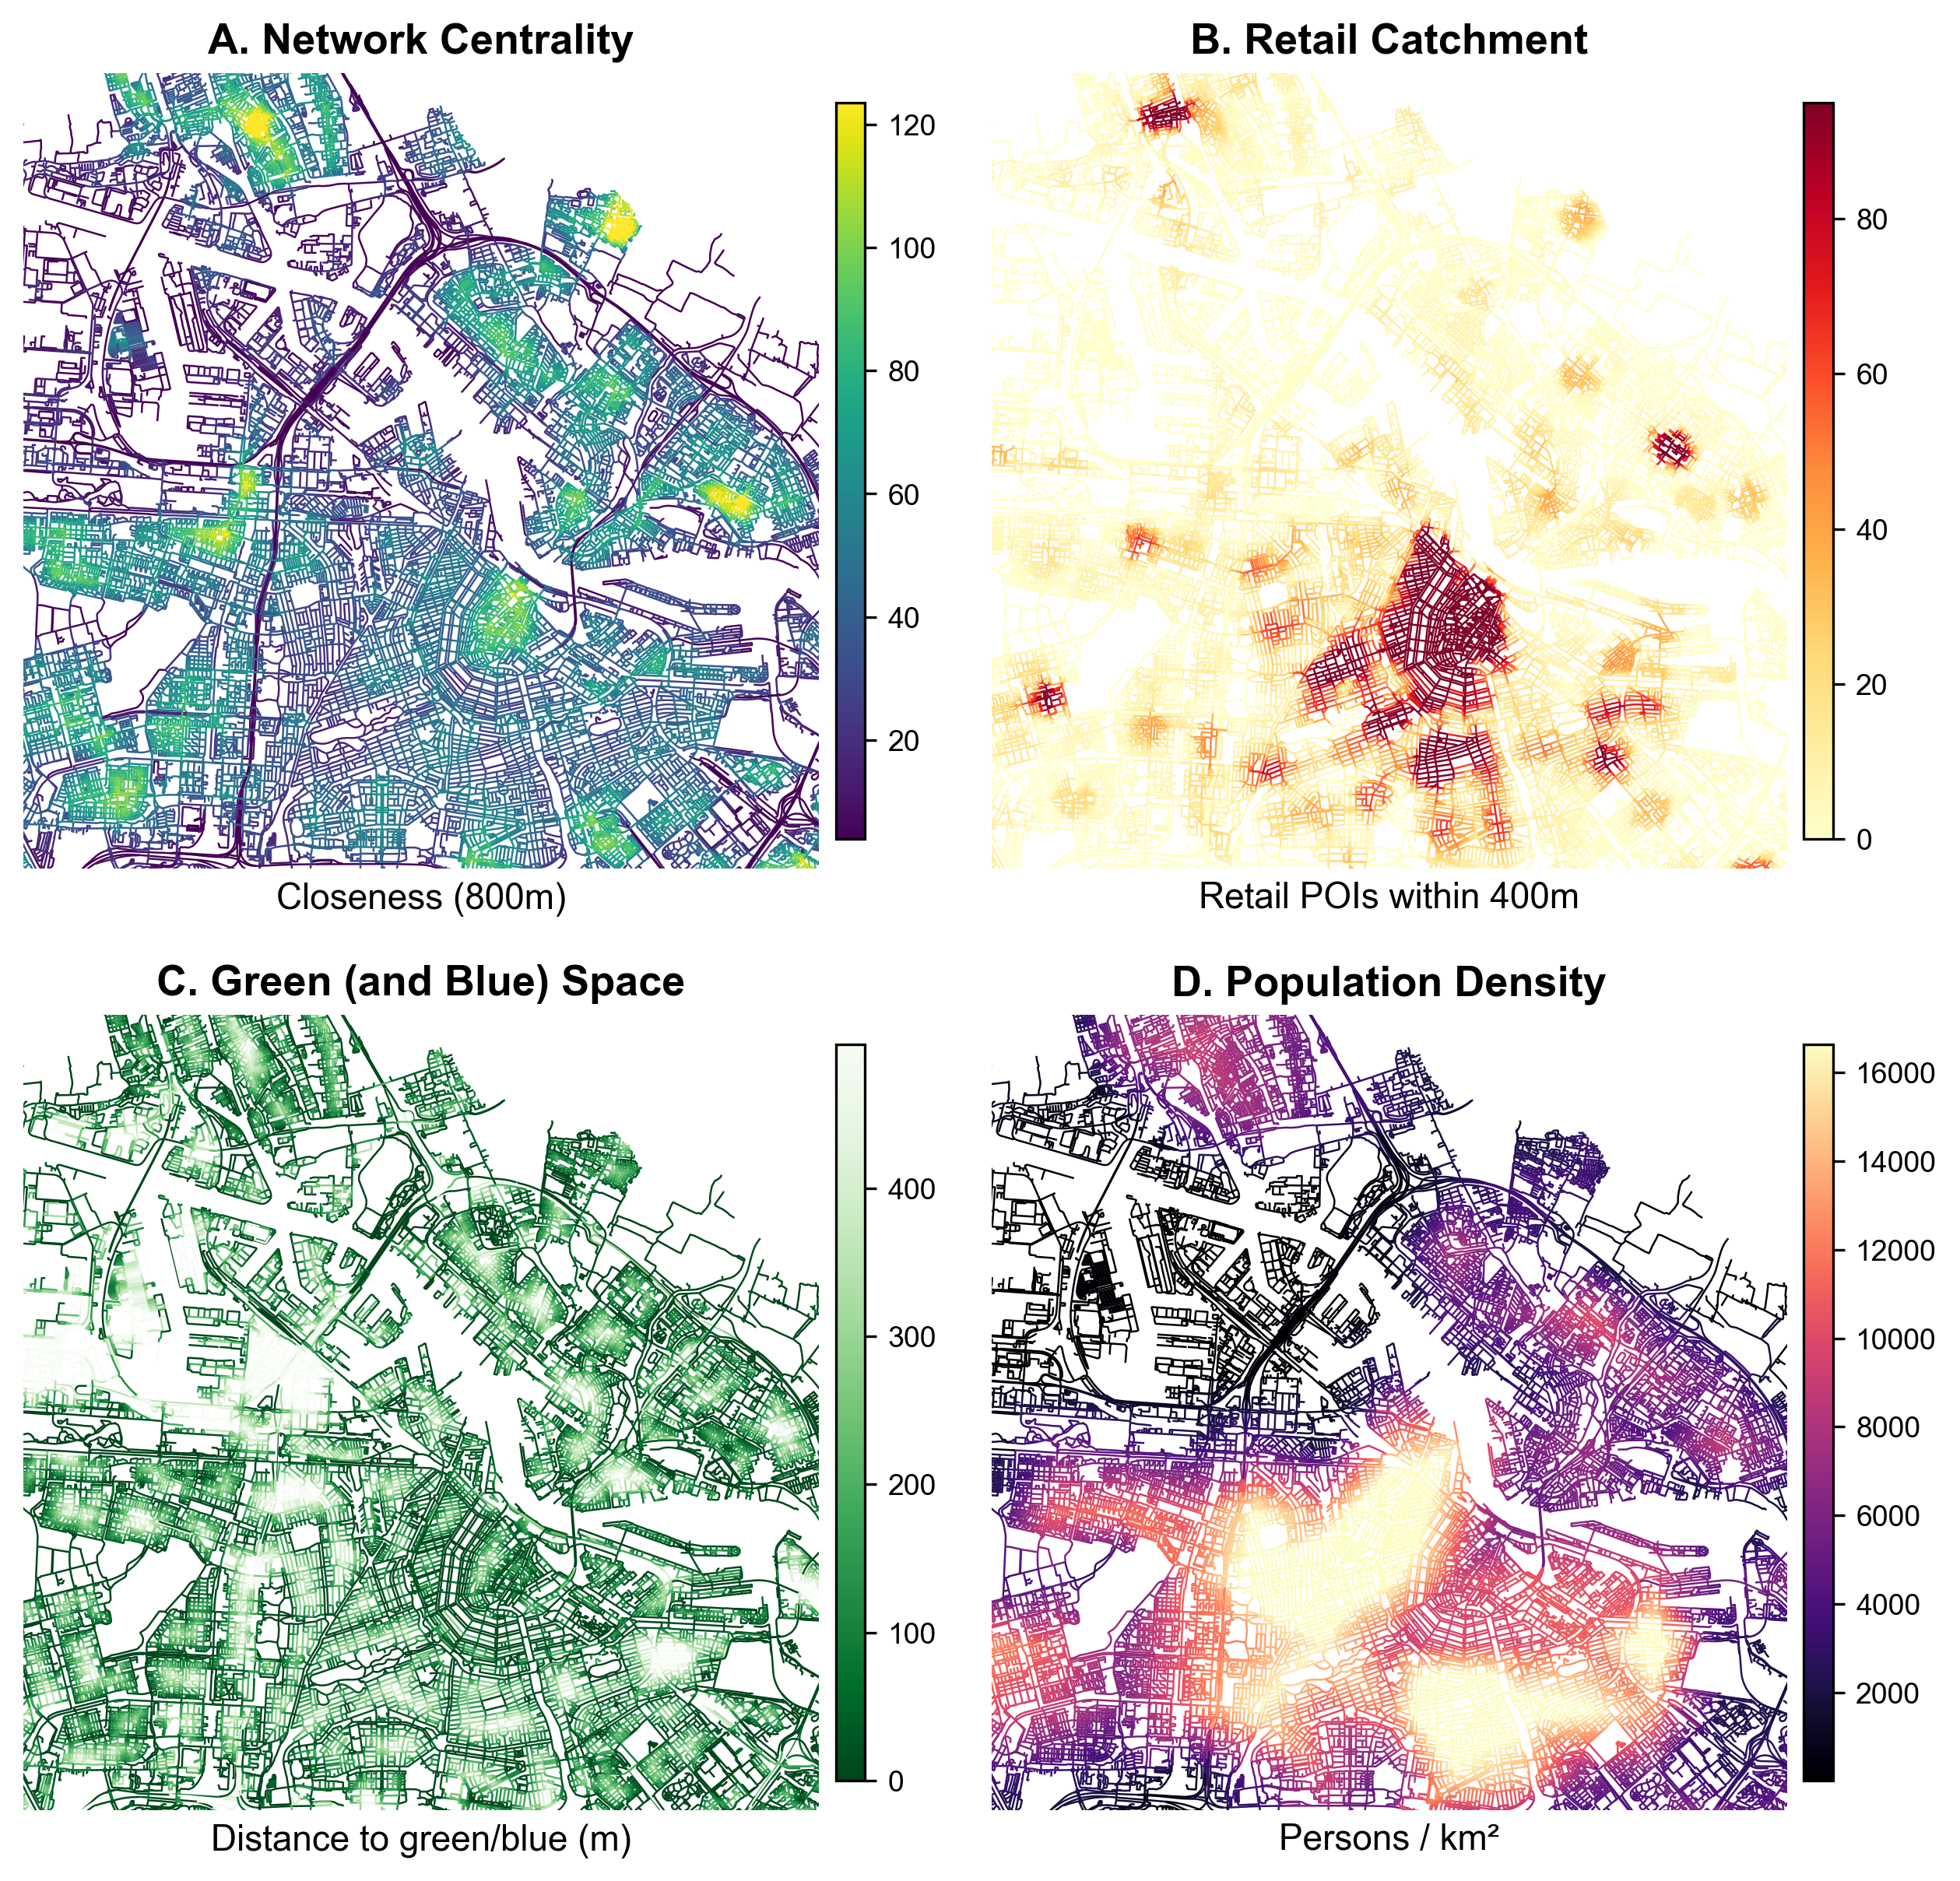
\includegraphics[width=\textwidth]{outputs/figures/fig_example_amsterdam.png}
  \caption{\textbf{Example SOAR-EU output for Amsterdam, Netherlands.} Street segments coloured by computed metrics: (A) closeness centrality at 800\,m threshold; (B) retail catchment (POI count within 400\,m); (C) distance to nearest green or blue space; (D) population density (persons/km\textsuperscript{2}, Eurostat Census Grid 2021). Different spatial scales and metric types lend themselves to different forms of analysis.}
  \label{fig:example-amsterdam}
\end{figure}

%% ============================================================================
%% METHODS
%% ============================================================================
\section{Methods}

Sections~\ref{sec:study-area}--\ref{sec:implementation} describe the processing pipeline (Figure~\ref{fig:pipeline}); Section~\ref{sec:provenance} discusses data provenance and source quality; Section~\ref{sec:poi-pattern-characterisation} provides scale-dependent usage guidance for POI-derived metrics. All source datasets were ingested during mid 2026 using the release versions indicated in Table~\ref{tab:sources}; the final dataset snapshot used for validation and distribution corresponds to Zenodo deposit \ZenodoDoi{}.

\begin{figure}[htbp]
  \centering
  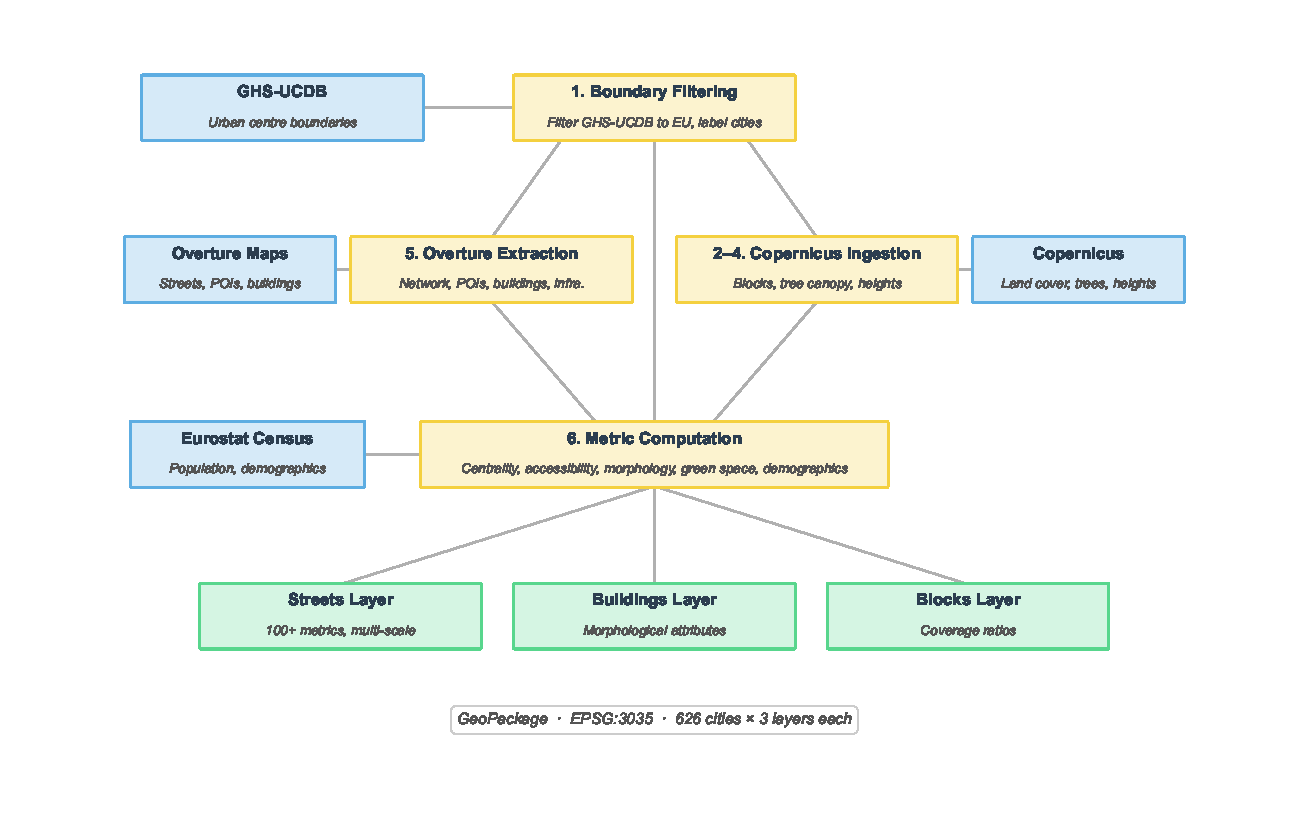
\includegraphics[width=0.85\textwidth]{outputs/figures/fig_pipeline.pdf}
  \caption{\textbf{SOAR-EU processing pipeline.} Four open data sources (blue) feed four processing stages (yellow) that produce three GeoPackage output layers per city (green). Stage~1 filters GHS-UCDB boundaries to the EU and labels cities; Stages~2--5 ingest Copernicus and Overture data in parallel; Stage~6 computes all metrics using the ingested layers, Eurostat census data, and the filtered boundaries.}
  \label{fig:pipeline}
\end{figure}

\subsection{Study Area Definition}
\label{sec:study-area}

Urban boundaries derive from the Global Human Settlement Layer Urban Centre Database (GHS-UCDB) R2024A \cite{ghsl2024}, which defines urban centres using the Degree of Urbanisation (DEGURBA) methodology: contiguous 1$\times$1~km grid cells with $\geq$1,500 inhabitants/km\textsuperscript{2} (or $\geq$50\% built-up surface) and cumulative population $\geq$50,000. Filtering to continental Europe (EPSG:3035) yielded \NCitiesTotal{} urban centres. All meet the $\geq$50,000 population threshold and thus correspond to cities or major urban agglomerations rather than small towns. City names are taken directly from the GHS-UCDB \texttt{GC\_UCN\_MAI\_2025} (Main Urban Centre Name) attribute. Because GHS-UCDB boundaries reflect population density contours rather than administrative units, assigned names may not always correspond to commonly used city names (e.g., a district name rather than the parent municipality).

\subsection{Data Sources}

Table~\ref{tab:sources} summarises input datasets.

Street networks from Overture Maps \cite{overture2026} were cleaned via cityseer \cite{simons2023}, following the automated network-cleaning procedure described in \cite{abdeldayem2026}: disconnected components were removed and degree-2 nodes collapsed. Level-aware processing prevents incorrect merging at bridges or tunnels. The 8\,m cleaning tolerance is deliberately conservative, prioritising consistent processing across all cities over city-specific fine-tuning.

POI categories from Overture's ``places'' theme were mapped to 11 analytical classes (Table~\ref{tab:landuse}; derivation in Section~\ref{sec:landuse-access}), and infrastructure points from Overture's infrastructure theme to three categories (transport, parking, street furniture; Table~\ref{tab:infrastructure}). Land cover and tree canopy derive from Copernicus Urban Atlas \cite{eea2021ua} and Street Tree Layer \cite{eea2021stl} respectively. Building heights were sampled from the Digital Height Model \cite{eea2012bh}.

Demographics from Eurostat Census Grid 2021 \cite{eurostat2024} include population, employment, age structure, nationality, and migration at 1~km\textsuperscript{2} resolution.

\begin{table}[H]
  \centering
  \caption{Input data sources and their roles in the processing pipeline.}
  \label{tab:sources}
  \small
  \begin{tabular}{@{}L{2.5cm}L{1.6cm}L{1cm}L{2.8cm}L{3.2cm}@{}}
    \toprule
    \textbf{Dataset} & \textbf{Source} & \textbf{Year} & \textbf{Licence} & \textbf{Use} \\
    \midrule
    GHS-UCDB R2024A & JRC/GHSL & 2024 & \href{https://commission.europa.eu/legal-notice_en\#copyright-notice}{EC reuse policy} & Urban boundaries \\
    Street networks & Overture Maps & 2026 & \href{https://opendatacommons.org/licenses/odbl/1-0/}{ODbL} & Centrality, accessibility \\
    Points of interest & Overture Maps & 2026 & \href{https://cdla.dev/permissive-2-0/}{CDLA-Permissive-2.0} & Land-use metrics \\
    Building footprints & Overture Maps & 2026 & \href{https://opendatacommons.org/licenses/odbl/1-0/}{ODbL} & Morphology \\
    Urban Atlas & Copernicus & 2021 & \href{https://land.copernicus.eu/en/data-policy}{Copernicus data policy} & Blocks, green space \\
    Street Tree Layer & Copernicus & 2021 & \href{https://land.copernicus.eu/en/data-policy}{Copernicus data policy} & Tree proximity \\
    Height Model & Copernicus & 2012 & \href{https://land.copernicus.eu/en/data-policy}{Copernicus data policy} & Building heights \\
    Census Grid & Eurostat & 2021 & \href{https://commission.europa.eu/legal-notice_en\#copyright-notice}{EC reuse policy} & Demographics \\
    \bottomrule
  \end{tabular}
\end{table}

\subsection{Data Processing Pipeline}

The pipeline comprises six stages executed via Python modules (Table~\ref{tab:pipeline}). All scripts support idempotent execution (existing outputs are skipped unless \texttt{overwrite} is specified), enabling incremental processing and failure recovery.

\begin{table}[H]
  \centering
  \caption{Processing pipeline stages with corresponding Python modules.}
  \label{tab:pipeline}
  \small
  \begin{tabular}{@{}cL{6cm}L{6cm}@{}}
    \toprule
    \textbf{Stage} & \textbf{Module} & \textbf{Description} \\
    \midrule
    1 & \texttt{src.data.generate\_boundary\_polys} & Filter GHS-UCDB boundaries to continental Europe \\
    2 & \texttt{src.data.load\_urban\_atlas\_blocks} & Extract Urban Atlas blocks per boundary \\
    3 & \texttt{src.data.load\_urban\_atlas\_trees} & Extract Street Tree Layer per boundary \\
    4 & \texttt{src.data.load\_bldg\_hts\_raster} & Clip building height rasters per boundary \\
    5 & \texttt{src.data.load\_overture} & Extract Overture data (network, POIs, buildings, infrastructure) \\
    6 & \texttt{src.processing.generate\_metrics} & Compute all metrics per boundary \\
    \bottomrule
  \end{tabular}
\end{table}

For accurate metric computation at boundary edges, input datasets are buffered beyond city boundaries. Street networks are buffered by 10\,km, giving nodes near boundaries a complete network context for centrality calculations. Points of interest, buildings, and infrastructure are buffered by 2\,km, capturing all reachable amenities for boundary-proximate locations. Copernicus land cover and tree canopy data is clipped to boundary bounding boxes for green-space proximity coverage.

\subsection{Metric Computation}
\label{sec:metric-computation}

\subsubsection{Network Centrality}
Network centrality metrics quantify a location's connectivity within the street network and were computed using the cityseer package \cite{simons2023}.

Closeness variants measure how accessible a location is relative to the rest of the network: beta-weighted closeness (gravity index with exponential distance decay), harmonic closeness (sum of inverse distances), Hillier-type closeness (node count divided by average node distance), farness (sum of distances), and street segment density. The density measure (\texttt{cc\_density\_DDD}) is an unweighted count of network nodes, each corresponding to a natural street-segment midpoint after cleaning, reachable within the network-distance threshold; it is not weighted by segment lengths. Betweenness centrality measures how often a location lies on shortest paths between other locations and is computed in both standard and distance-weighted forms.

Metrics were generated using cityseer's shortest-path centrality (\texttt{centrality\_shortest}) at thresholds of 400\,m, 800\,m, 1,200\,m, 1,600\,m, 4,800\,m, and 9,600\,m, corresponding to 5--120 minute walking catchments at 80\,m/min average pedestrian speed. These thresholds span local-to-global catchments: 400\,m captures immediate neighbourhood context; 800\,m reflects typical distances walked to transit; the 1,200--1,600\,m range corresponds to 15-minute walking catchments; 4,800\,m characterises district-scale network structure; and 9,600\,m extends to city-wide connectivity. Centralities are measured using shortest paths (as opposed to angular paths) for greater tolerance of artefacts deriving from automated street cleaning procedures.

\subsubsection{Land-Use and Infrastructure Accessibility}
\label{sec:landuse-access}
Points of interest from Overture Maps were classified into the 11 aggregated land-use categories distributed with the dataset (Table~\ref{tab:landuse}). The aggregation follows Overture's own top-level groupings to the extent possible, rather than imposing a re-engineered taxonomy: most of the 11 categories correspond directly to a single Overture top-level class, with only two consolidations (\texttt{eat\_and\_drink} merging restaurants, bars, and cafés; \texttt{business\_and\_services} merging eleven Overture professional and commercial sub-classes) and two renames (\texttt{public\_services} from \texttt{public\_service\_and\_government}, \texttt{religious} from \texttt{religious\_organization}). The complete mapping from Overture's 2,000+ leaf categories to analytical classes is detailed in Supplementary Material (Section~S2).

Overture's separate infrastructure theme is grouped into three further accessibility categories (transport, parking, and street furniture; Table~\ref{tab:infrastructure}), which receive the identical network-accessibility treatment described below.

Accessibility metrics aggregate POI counts over the street network at the same street-segment locations used for centrality computations, enabling direct comparison between network structure and land-use distribution \cite{simons2023}. Network-based distances are used throughout, rather than Euclidean buffers or zonal aggregation.

For each land-use and infrastructure category, both unweighted counts (reachable POIs within $d_{\max}$) and distance-weighted counts (applying exponential decay $e^{-\beta d}$, where $\beta = 4/d_{\max}$ such that weight falls to approximately 0.018 at the distance threshold) were computed, alongside nearest-distance measures. Distance-weighted counts reflect how amenity usage decays with distance (a caf\'{e} at 100\,m contributes more than one at 1,000\,m), while unweighted counts offer simpler interpretability.

The exponential weight never reaches zero, so an establishment infinitely far would still make an infinitesimal contribution. To keep each measure finite and tied to a walkable catchment, a threshold distance $d_{\max}$ is imposed rather than integrating over the entire network. The decay rate is set at $\beta = 4/d_{\max}$ where the weight has already fallen to under 2\% by the time it reaches $d_{\max}$, thereby discarding the infinitely long tail with minimal impact on the aggregations. The threshold distances are chosen for rounding convenience and the provision of a range of thresholds lets users choose the catchment that suits the intended usage scenario.

Mixed-use diversity was quantified using Hill numbers \cite{hill1973}. Hill numbers at $q=0$ equal richness (count of distinct land-use types); at $q=1$, the exponential of Shannon entropy; at $q=2$, the inverse Simpson index. We compute all three variants in both unweighted and distance-weighted forms, where the distance-weighted forms follow the same weighting conventions as described for land-use accessibility.

\subsubsection{Morphology}
Building and block morphology metrics were computed using the momepy package \cite{fleischmann2019}, which provides standardised urban morphometric functions.

For each building footprint, we compute: area, perimeter, circular compactness, orientation, corners count, shape index, fractal dimension, and shared wall ratio (fraction of perimeter shared with adjacent buildings). Building heights are extracted from the Copernicus Height Model raster by buffering each footprint by 10\,m (one DHM pixel) and averaging valid (non-null) overlapping pixel values. The single-pixel buffer ensures that small footprints (those contained within a single pixel) and footprints with minor misregistration against the 2012 raster still receive a height sample; the trade-off is some smoothing in dense fabric where party-wall neighbours and narrow courtyards fall within the buffer. The height value enables computation of volume and form factor. Floor area (assuming 3\,m floor height) is computed per building as an intermediate for block-level FSI but is not retained as a standalone aggregated metric.

Block morphology uses only built-up Urban Atlas blocks: 14 non-built land-cover classes (green areas, forests, agriculture, water, wetlands, and sports/leisure facilities) are excluded before morphometric computation and aggregation of the metrics to the adjacent streets. For the remaining blocks, we compute geometric properties (area, perimeter, circular compactness, orientation) and Spacematrix indicators \cite{haupt2010}: ground space index (GSI, building footprint area divided by block area), floor space index (FSI, total floor area divided by block area), open space ratio (OSR $= (1 - \text{GSI}) / \text{FSI}$), mean number of storeys (L $= \text{FSI} / \text{GSI}$), and area-weighted mean building height. Blocks exceeding 2\,km\textsuperscript{2} are additionally excluded as oversized infrastructural or transitional polygons (the threshold separates typical urban blocks from large airport, port, industrial, or transitional polygons that occur in the Urban Atlas layer); blocks below 1\% building coverage receive NaN for all Spacematrix metrics, since the ratios become numerically unstable as their denominators (GSI, FSI) approach zero.

Building and block metrics are aggregated to streets via nearest-network-distance assignment within 200\,m and 400\,m thresholds. Each building or block centroid is assigned to the nearest street, and statistics (median and median absolute deviation) are computed across all features within each threshold distance. For building area and volume, sum statistics are additionally retained; for block area, only the sum is additionally retained. Building height is also aggregated (as median and MAD of individual building heights per street).

In addition, a bilateral street-frontage ratio is computed per street segment as a source-robust measure of building continuity. For each street, a 35\,m buffer defines a corridor; all building edges whose midpoint falls inside the corridor and whose nearest street is this one are identified. Per side (left/right of the centreline), only edges within 5\,m of the closest edge are retained, filtering out rear extensions and garages while preserving the primary facade line. The score is the fraction of street length covered by the retained edges on the more-covered side (3\,m trimmed from each end as a junction guard). Unlike shared wall ratio, which requires exact topological contact between adjacent polygon boundaries, frontage ratio depends only on building \emph{presence} along the street edge. It is therefore insensitive to unintended gaps and to the lack of delineation between neighbouring buildings that is characteristic of ML-derived footprints, where segmentation pipelines lack the cadastral subdivision information available to community-contributed sources (see Section~\ref{sec:provenance}).

\subsubsection{Green Space Proximity}
Network distance to nearest green space polygon edge was computed for each street. Green spaces derive from 12 Urban Atlas land cover classes: public and unknown-access urban green areas, forests, herbaceous vegetation, open spaces with little or no vegetation, wetlands, water bodies, pastures, arable land, permanent crops, mixed cultivation, and orchards (full list in Supplementary Material Section~S3). Sports and leisure facility blocks often function as green space (e.g., open playing fields) but can also be heavily built up (e.g., stadiums, indoor arenas); we therefore apply a consistent 20\% building-coverage threshold, including the block as green space when built coverage is below 20\% and excluding it otherwise.

Polygon boundaries are sampled at 20\,m intervals to generate point features for distance calculations, improving accuracy for large or irregularly-shaped polygons. For each street, only the distance to the single nearest sampled point is retained, so a polygon contributes to a given street at most once regardless of how many of its boundary samples lie within range. Tree canopy proximity uses Street Tree Layer polygons with equivalent sampling. Green space and tree canopy areas are also aggregated within walking distances (200\,m, 400\,m, 800\,m) to quantify local coverage.

\subsubsection{Demographic Interpolation}
Census grid values were interpolated to street-segment midpoints using Delaunay-based linear barycentric interpolation (\texttt{scipy.interpolate.griddata}, method \texttt{linear}) from 1\,km grid cell centroids. Interpolated variables include: total population (\texttt{t}), population density (\texttt{density}), male/female counts (\texttt{m}, \texttt{f}), age cohorts (\texttt{y\_lt15}, \texttt{y\_1564}, \texttt{y\_ge65}), employment (\texttt{emp}), nationality (\texttt{nat}, \texttt{eu\_oth}, \texttt{oth}), and migration flows (\texttt{same}, \texttt{chg\_in}, \texttt{chg\_out}). Percentage variants (suffixed with \texttt{\_\%}) are computed for each variable relative to total population. Linear interpolation from 1\,km\textsuperscript{2} source cells produces smooth gradients that do not represent sharp sub-cell discontinuities (industrial estates, large parks, transit corridors); these street-level demographic values should be read as neighbourhood-scale context rather than as fine-grained block-level estimates.

\subsection{Implementation}
\label{sec:implementation}

The pipeline is implemented in Python 3.12 with modules for data ingestion, metric processing, utilities, and land-use classification. Network loading retrieves Overture ``connector'' and ``segment'' themes via STAC, transforms to EPSG:3035, and applies cityseer cleaning (8\,m tolerance, 100-node minimum component size). POI loading maps Overture's 2,000+ raw categories to 23 intermediate classes via a CSV lookup (preserved in the code repository for transparency and reuse), which are then aggregated to the 11 analytical categories distributed with the dataset (Table~\ref{tab:landuse}).

Table~\ref{tab:parameters} summarises the fixed processing parameters ensuring reproducibility across all urban centres.

\begin{table}[!htbp]
  \centering
  \caption{Fixed processing parameters for reproducibility.}
  \label{tab:parameters}
  \small
  \begin{tabular}{@{}L{4cm}L{3cm}L{4.5cm}@{}}
    \toprule
    \textbf{Parameter} & \textbf{Value(s)} & \textbf{Rationale} \\
    \midrule
    Network cleaning tolerance & 8\,m & Consolidate near-parallel edges \\
    Min.\ component size & 100 nodes & Remove disconnected fragments \\
    Centrality thresholds & 400, 800, 1200, 1600, 4800, 9600\,m & 5--120 minute walking catchments \\
    Accessibility thresholds & 200, 400, 800, 1200, 1600\,m & Pedestrian-scale proximity \\
    Morphology aggregation & 200, 400\,m & Immediate building context \\
    Green space proximity & 1600\,m & Extended walkable distance \\
    Green area aggregation & 200, 400, 800\,m & Multi-scale green coverage \\
    \bottomrule
  \end{tabular}
\end{table}

Outputs are written as GeoPackage files in EPSG:3035 following the structure described in Section~\ref{sec:dataset-structure}. Dependencies are pinned via \texttt{pyproject.toml}; core packages include cityseer, momepy, geopandas, and overturemaps.

\subsection{Data Provenance}
\label{sec:provenance}

SOAR-EU integrates data layers with different provenance. Eurostat boundaries, census data, and Copernicus land cover follow documented methodologies with full pan-European coverage. Street networks derive from OpenStreetMap via Overture, whose road coverage is largely complete across urbanised Europe \cite{barringtonleigh2017}.

Building footprints derive from Overture Maps, which conflates multiple sources in a fixed priority order: community-contributed datasets (OpenStreetMap, Esri Community Maps, national cadastres) take precedence over ML-derived datasets (Microsoft ML Building Footprints, Google Open Buildings). When two sources contain the same building (IoU~$\geq$~50\%), the higher-priority source's geometry is retained; ML-derived footprints fill areas not covered by community sources. Each footprint carries a \texttt{sources} attribute recording which dataset contributed it, enabling downstream filtering by provenance.

In European cities, OpenStreetMap is typically the dominant contributor. Herfort et al.\ \cite{herfort2023} analysed OSM building completeness across 13{,}189 urban agglomerations worldwide and found Europe and Central Asia to have the highest regional average (71\%), though within-region coverage remains uneven. Countries with completed cadastral imports---France (DGFiP cadastre), the Netherlands (BAG), and Belgium/Flanders (GRB)---are generally considered to have a high degree of community-sourced building coverage. In contrast, several southern and eastern European countries (including Romania, Bulgaria, Greece, Hungary, and Portugal) lack such imports and, in our data, rely more heavily on Microsoft's ML-derived footprints. Such ML-derived footprints overlap imperfectly with reference building data \cite{minghini2024}, as they are segmented from imagery rather than digitised from cadastre. Across the \NCitiesTotal{} cities in SOAR-EU, the proportion of ML-derived footprints ranges from near-zero in countries with complete cadastral imports to substantial in several southern and eastern European countries; per-city and per-country breakdowns are provided in the accompanying \texttt{building\_source\_counts.csv} and \texttt{building\_source\_by\_country.csv} (summarised in Supplementary~\S\ref{sec:bldg-supp}), and per-city completeness can be cross-referenced against the ohsome OSM-completeness map at \url{https://hex.ohsome.org/#/urban_building_completeness}.

ML-derived footprints expand coverage but introduce quality trade-offs relevant to morphometric computation. Because they are segmented from overhead imagery rather than digitised from cadastral plans, they delineate roof outlines rather than ground-level footprints and can merge adjacent structures into single polygons or leave gaps that break the topological adjacency these metrics rely on. The effect is visible directly in our data: metrics that depend on exact polygon boundary coincidence (particularly shared wall ratio and, to a lesser extent, fractal dimension) are systematically affected, with shared wall ratio showing the strongest negative association between a city's ML fraction and its median value (full coefficients in Supplementary Table~\ref{tab:building_metric_sensitivity}; the within-city test in Supplementary~\S\ref{sec:bldg-supp} confirms this as a per-building artefact rather than a country-level morphological gradient). Metrics based on polygon area and shape (compactness, orientation, shape index) show no significant association with source composition.

POI data derives primarily from commercial and editorial sources (e.g., Meta, Microsoft, Foursquare, OSM) via Overture, with variable coverage relative to official registries; this is characterised in detail in Section~\ref{sec:poi-pattern-characterisation}. Temporal currency and other cross-layer caveats are summarised under Limitations of the Dataset.

\subsection{POI-derived accessibility: source-substitution analysis}
\label{sec:poi-pattern-characterisation}

Because Overture's POI layer aggregates commercial and crowdsourced data of varying completeness, the reliability of derived metrics varies across categories and spatial scales. To characterise where agreement holds and where it does not, we recompute POI-derived outputs against independent official registries in the two countries for which suitable national registries are openly available: France (SIRENE, \NRefCitiesFr{} cities) and the Netherlands (BAG, \NRefCitiesNl{} cities), \NRefCities{} reference cities in total. This validation therefore speaks directly to French and Dutch coverage; cities elsewhere in Europe (particularly in southern and eastern Europe, where OpenStreetMap-derived coverage is less mature) are outside its scope and should be treated with the additional caution discussed under Limitations of the Dataset. We frame the comparison around three questions that capture the main analytical uses of the resulting metrics:
\begin{itemize}
  \item \textbf{How many, relative to elsewhere?} Whether locations are ranked consistently by how much of a particular land use they can access. This is a pattern-agreement question as opposed to one of absolute counts: Overture is known to undercount relative to official registries (further discussed below), so the analytically useful question is whether that undercounting preserves the spatial ordering of accessibility.
  \item \textbf{Where are the hotspots?} Which locations fall in the top tier of activity.
  \item \textbf{How far is the nearest?} Whether the land use is reachable within a given distance threshold.
\end{itemize}
For each question, we measure agreement between Overture- and registry-derived accessibility for every street segment, then summarise within cities and across cities for each category and spatial scale (Figure~\ref{fig:pointa_support_heatmap}; Table~\ref{tab:pointa_minima}).

\subsubsection{Source-substitution replication}

\begin{figure}[!htb]
  \centering
  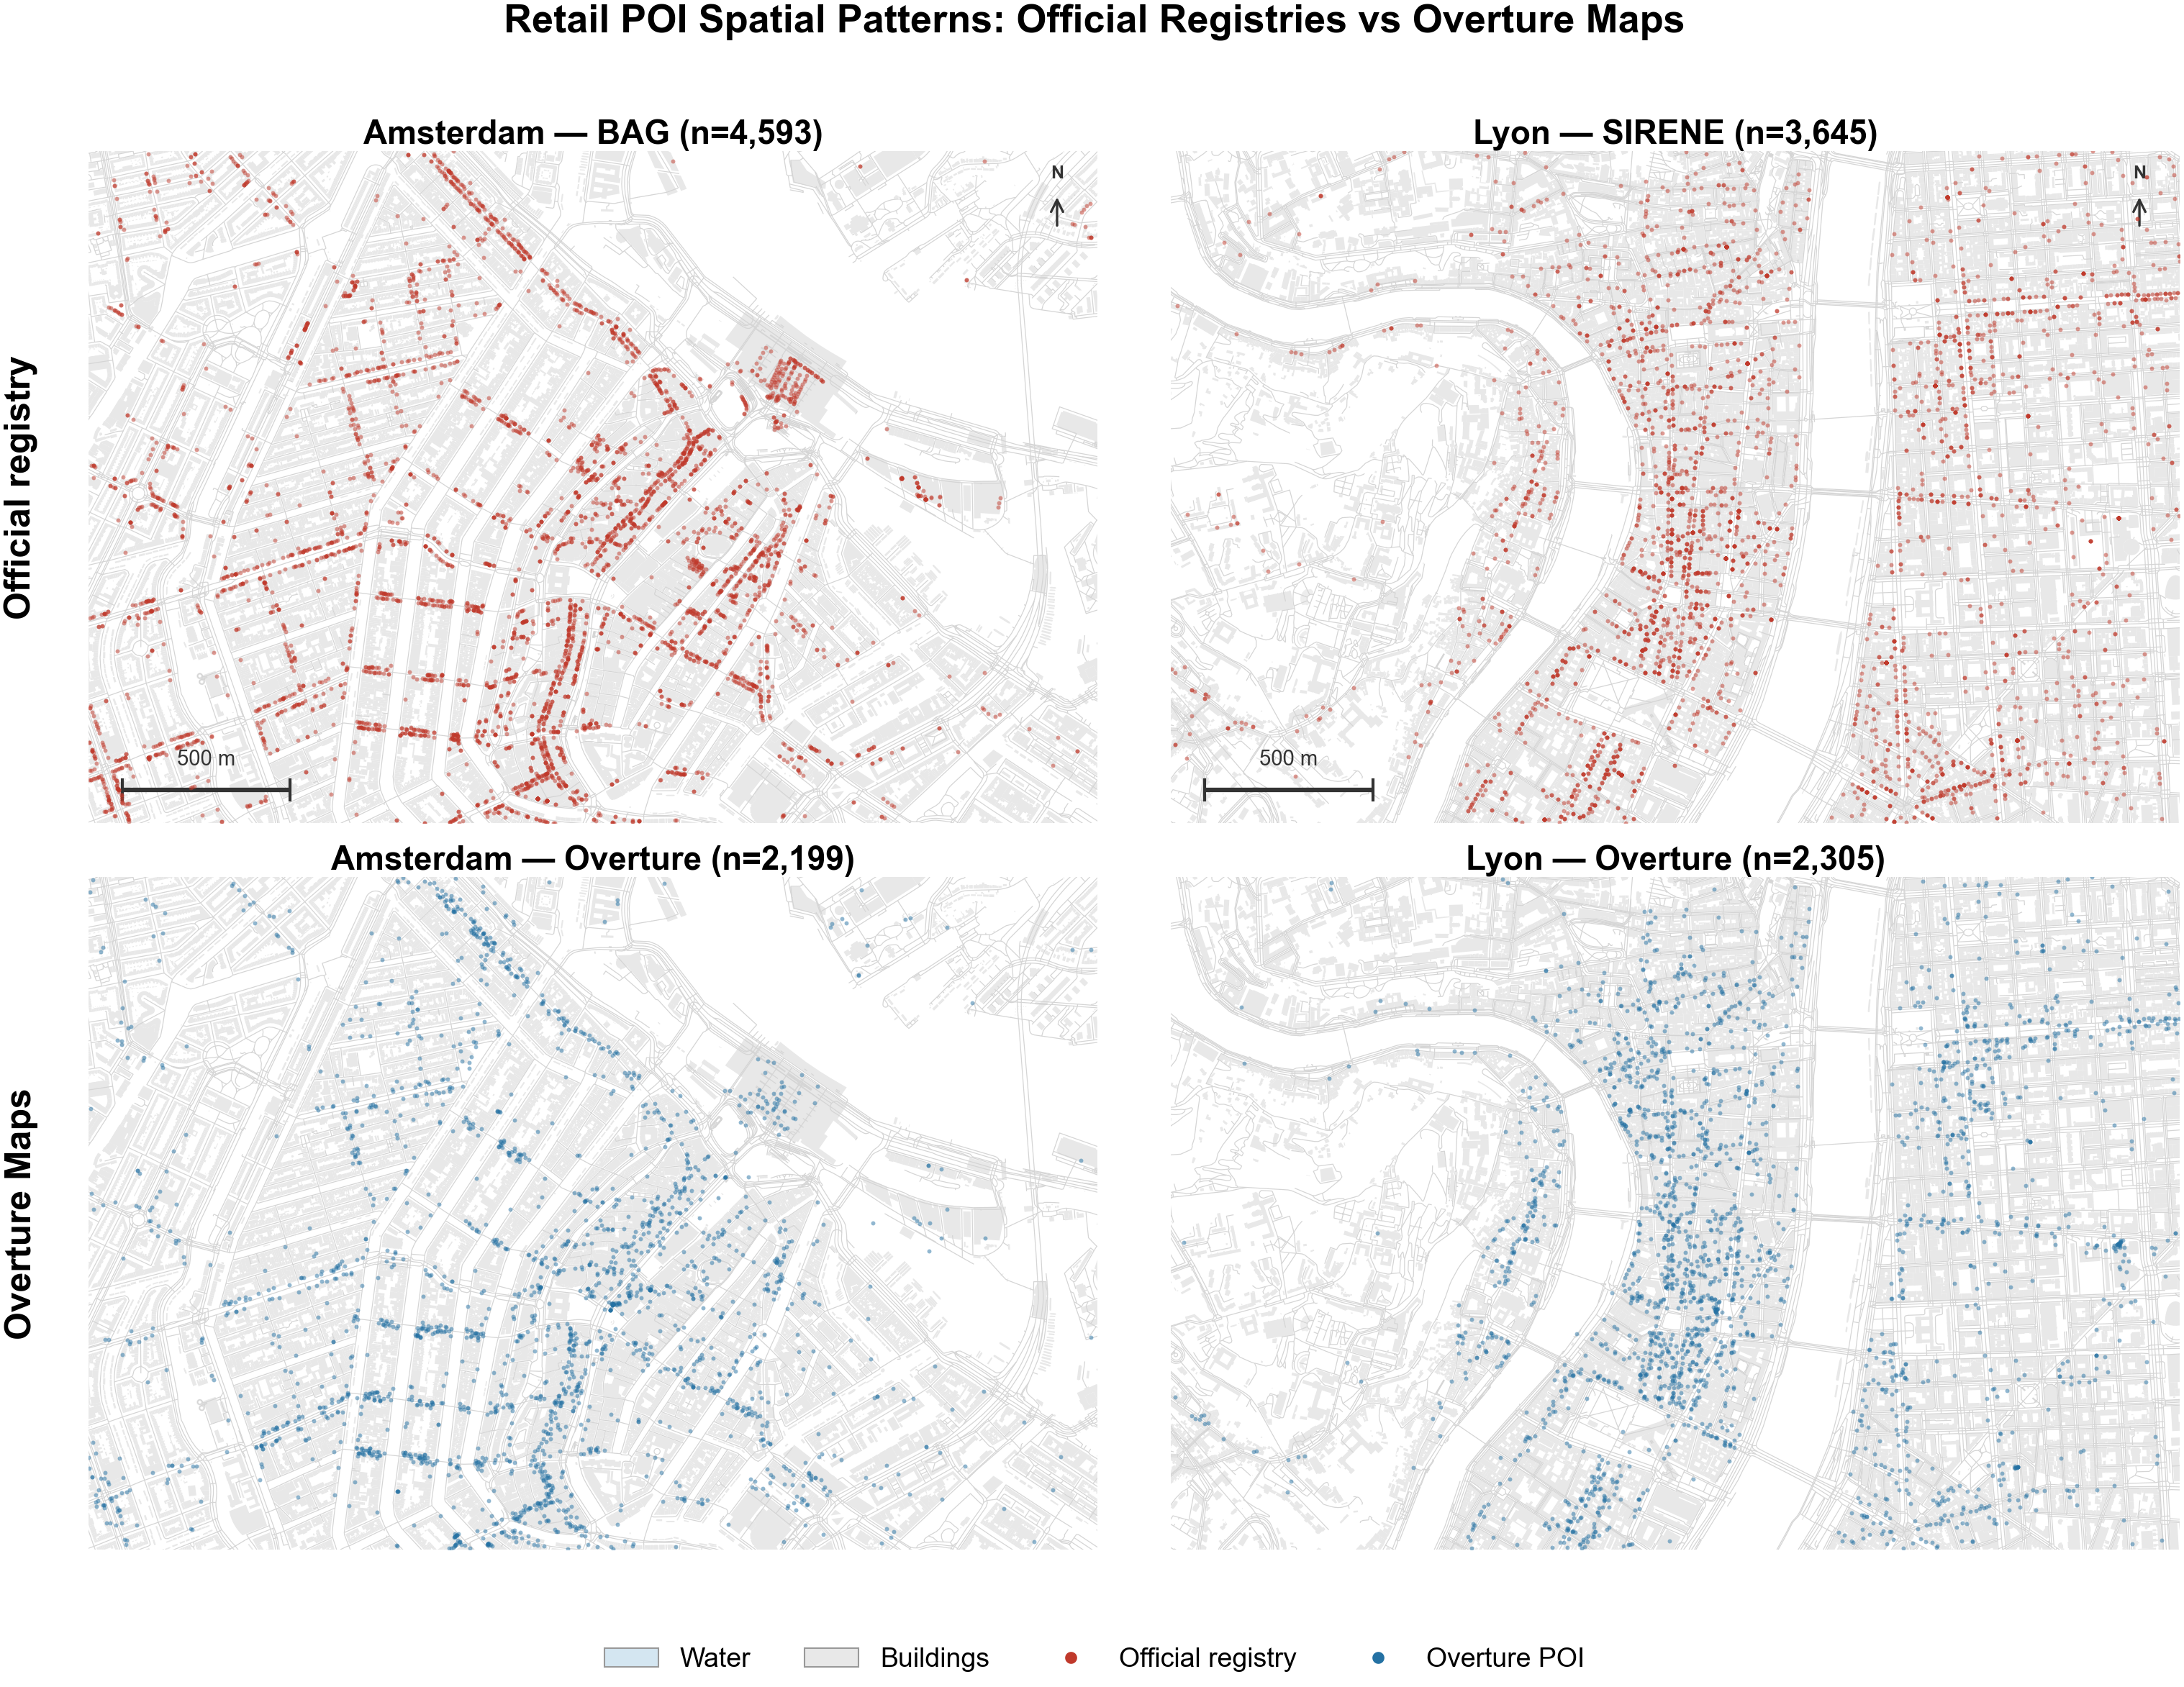
\includegraphics[width=\textwidth]{outputs/figures/fig_poi_spatial_comparison.png}
  \caption{\textbf{Retail POI locations from official registries (top) and Overture Maps (bottom)} for inner-city areas of Amsterdam (BAG; left) and Lyon (SIRENE; right). Point counts differ substantially between sources (Overture undercounts relative to the official registries), but the spatial clustering patterns are broadly consistent.}
  \label{fig:poi_spatial_comparison}
\end{figure}

\begin{figure}[p]
  \centering
  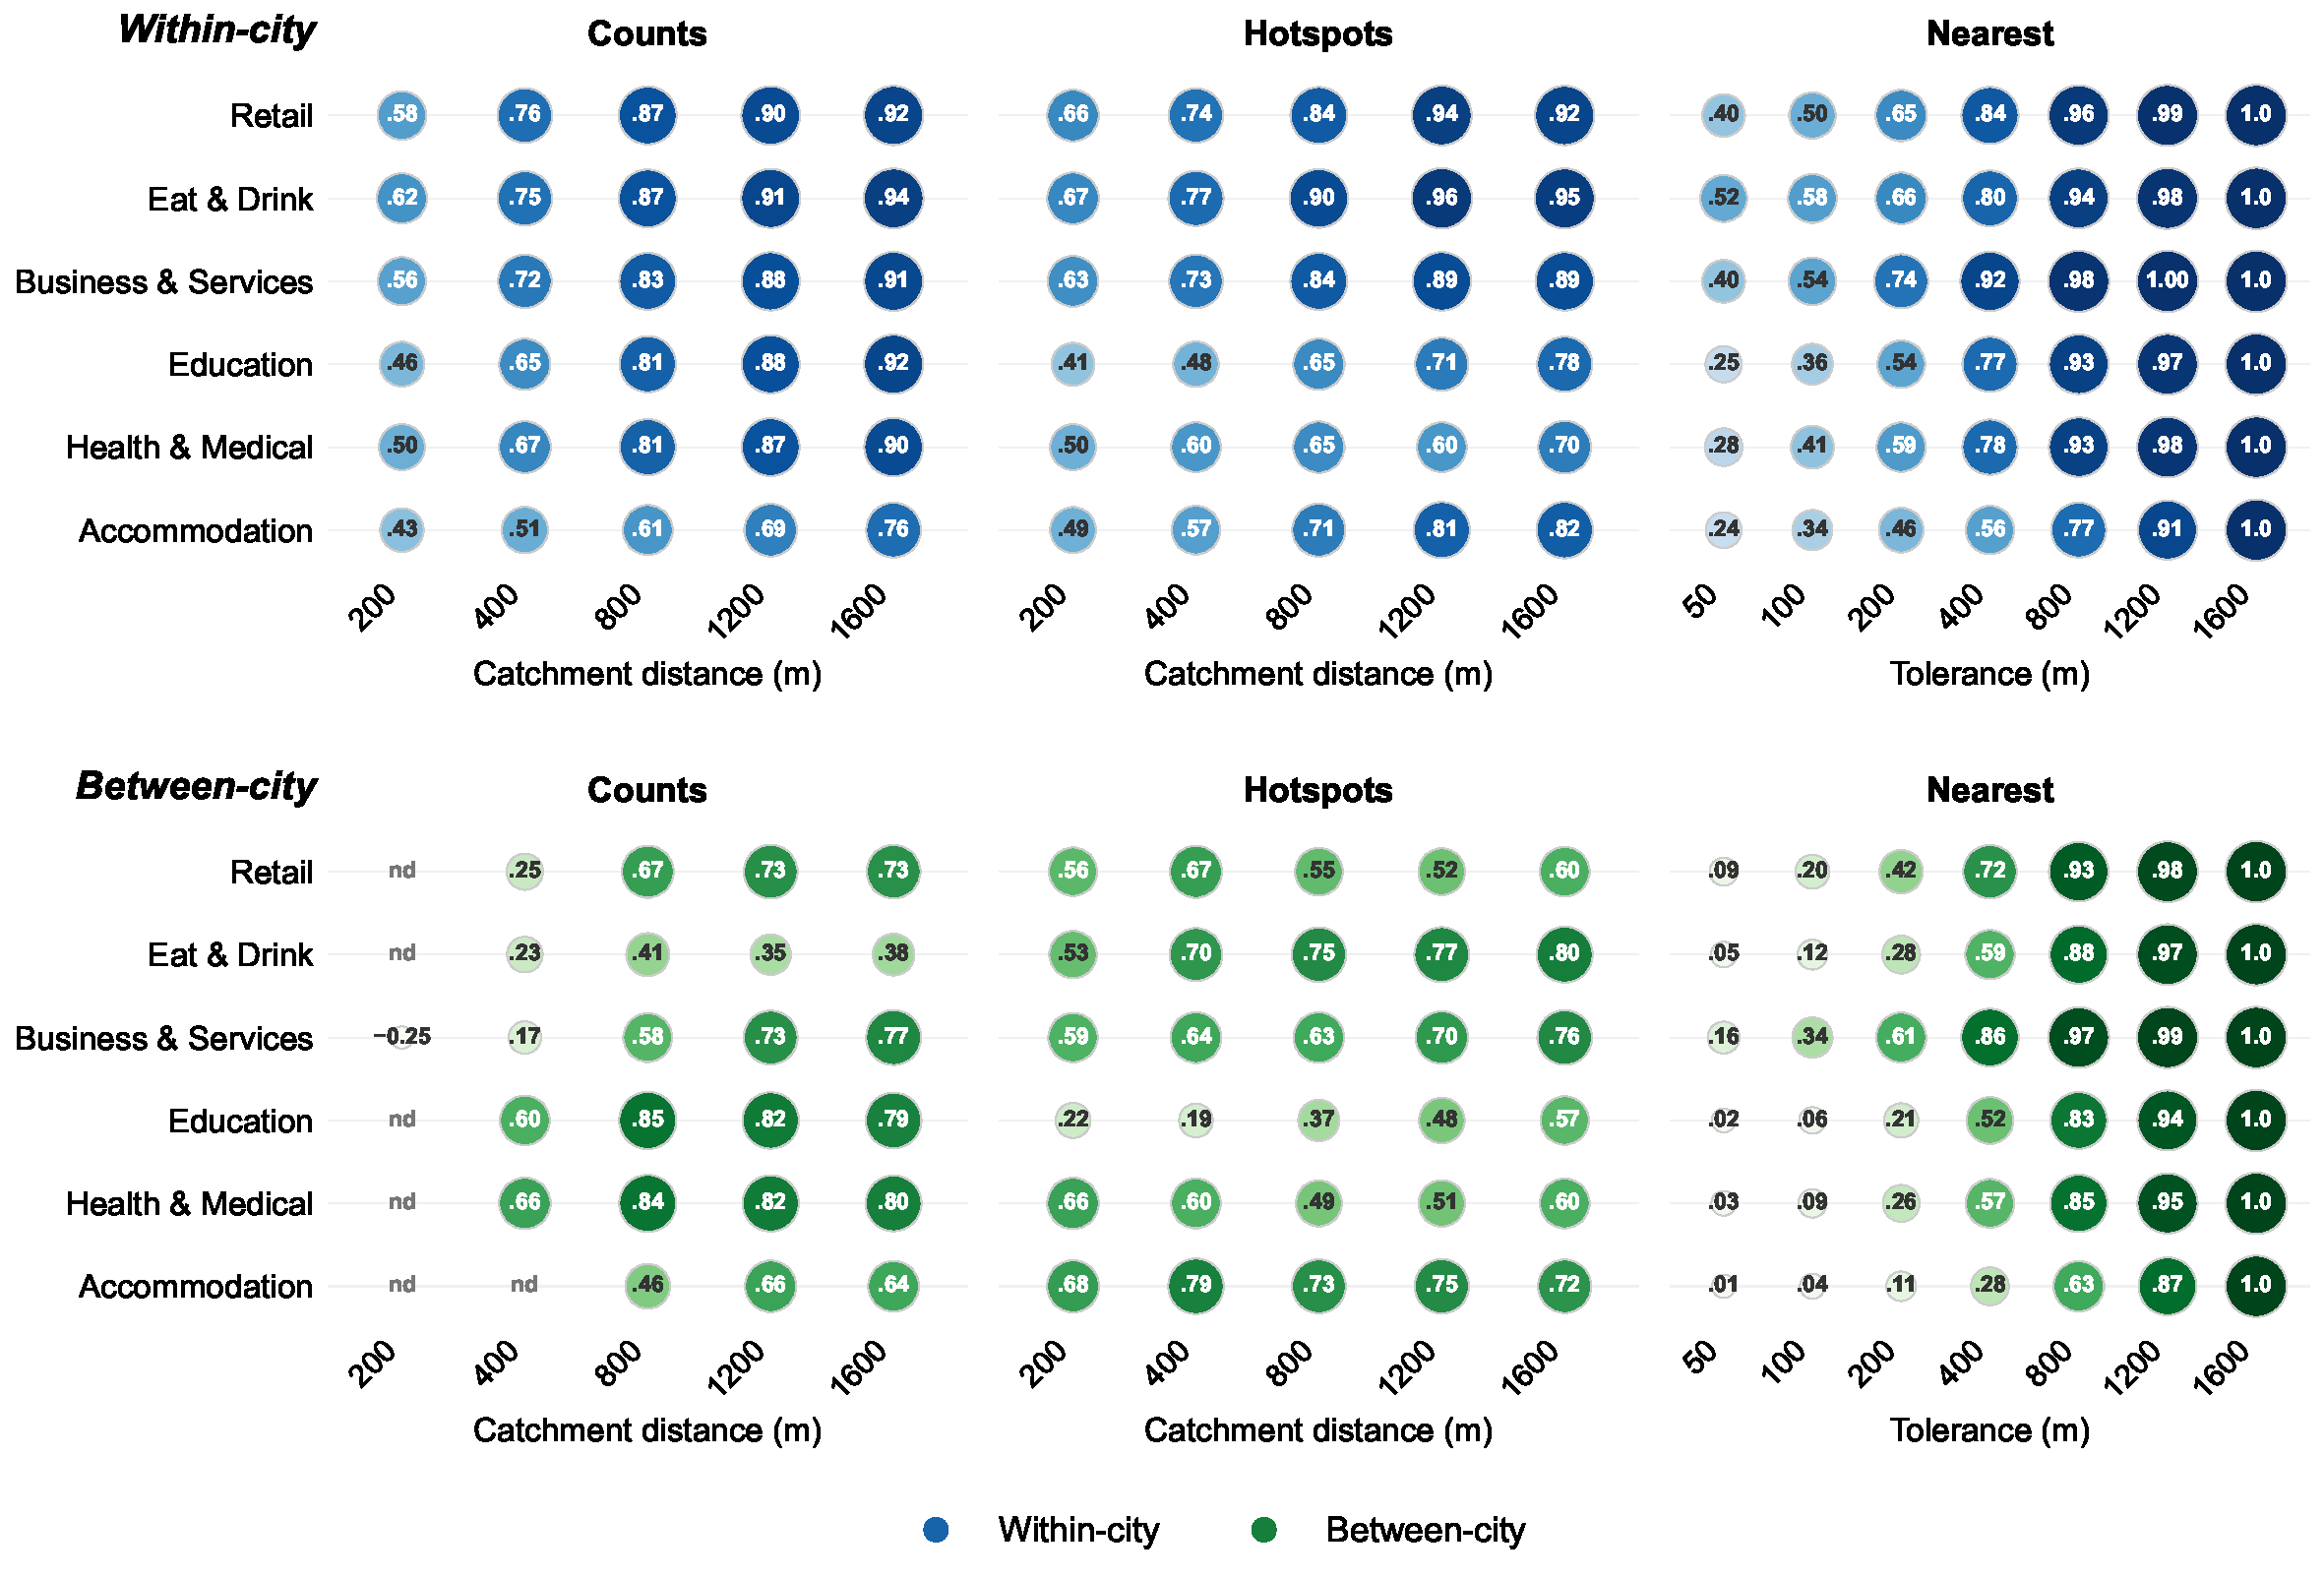
\includegraphics[width=\textwidth]{outputs/figures/fig_pointa_support_heatmap.pdf}
  \caption{\textbf{POI source-substitution agreement.}
    Agreement between Overture- and registry-based accessibility across all category--task--scale combinations. Top row (within-city): Spearman $\rho$ for segment-level rank correlation, top-10\% hotspot overlap, and nearest-distance F1. Bottom row (between-city): Spearman $\rho$ on city-level median counts and hotspot intensity, and harmonic-mean agreement of city-level nearest shares. Bubble size and annotation indicate the median score; colour distinguishes within-city from between-city scope. ``nd'' indicates insufficient data. Full agreement curves with bootstrap CIs appear in Supplementary Figure~\ref{fig:pointa_agreement_panels}.
  }
  \label{fig:pointa_support_heatmap}
\end{figure}

\begin{table}[p]
  \centering
  \caption{Minimum spatial scale (metres) at which each category's median agreement reaches $\geq$70\%, $\geq$75\%, $\geq$80\%, and $\geq$85\% concordance, grouped by scope (within-city, between-city) and metric family. For rank-correlation metrics, concordance is the fraction of observation pairs ranked identically by both sources, computed directly as $(1+\tau)/2$ where $\tau$ is the Kendall rank correlation (thresholds: $\tau \geq 0.40$, $0.50$, $0.60$, $0.70$). For overlap and F1 metrics the concordance fraction is used directly. Dashes indicate no tested scale reached that value.}
  \label{tab:pointa_minima}
  \scriptsize
  \begin{tabular}{@{}lcccccccccccc@{}}
\toprule
\textbf{Category} & \multicolumn{4}{c}{\textbf{Counts}} & \multicolumn{4}{c}{\textbf{Hotspots}} & \multicolumn{4}{c}{\textbf{Nearest}} \\
\cmidrule(lr){2-5}
\cmidrule(lr){6-9}
\cmidrule(lr){10-13}
 & $\geq$70\% & $\geq$75\% & $\geq$80\% & $\geq$85\% & $\geq$70\% & $\geq$75\% & $\geq$80\% & $\geq$85\% & $\geq$70\% & $\geq$75\% & $\geq$80\% & $\geq$85\% \\
\midrule
\textit{Within-city} & \multicolumn{4}{c}{\footnotesize rank concordance} & \multicolumn{4}{c}{\footnotesize top-10\% overlap} & \multicolumn{4}{c}{\footnotesize nearest F1} \\
Retail & 200 & 200 & 400 & 800 & 400 & 800 & 800 & 1200 & 400 & 400 & 400 & 800 \\
Eat \& Drink & 200 & 200 & 400 & 800 & 400 & 400 & 800 & 800 & 400 & 400 & 800 & 800 \\
Business \& Services & 200 & 400 & 800 & 1200 & 400 & 800 & 800 & 1200 & 200 & 400 & 400 & 400 \\
Education & 200 & 400 & 800 & 1200 & 1200 & 1600 & --- & --- & 400 & 400 & 800 & 800 \\
Health \& Medical & 200 & 400 & 800 & 1200 & 1600 & --- & --- & --- & 400 & 400 & 800 & 800 \\
Accommodation & 200 & 800 & 1600 & --- & 800 & 1200 & 1200 & --- & 800 & 800 & 1200 & 1200 \\
\midrule
\textit{Between-city} & \multicolumn{4}{c}{\footnotesize rank concordance (city medians)} & \multicolumn{4}{c}{\footnotesize rank concordance (hotspot intensity)} & \multicolumn{4}{c}{\footnotesize harmonic-mean share} \\
Retail & 800 & 800 & --- & --- & 200 & --- & --- & --- & 400 & 800 & 800 & 800 \\
Eat \& Drink & --- & --- & --- & --- & 200 & 400 & 1600 & --- & 800 & 800 & 800 & 800 \\
Business \& Services & 800 & 1200 & --- & --- & 200 & 1200 & --- & --- & 400 & 400 & 400 & 400 \\
Education & 400 & 400 & 800 & 800 & 1600 & --- & --- & --- & 800 & 800 & 800 & 1200 \\
Health \& Medical & 400 & 400 & 400 & --- & 200 & 200 & --- & --- & 800 & 800 & 800 & 800 \\
Accommodation & 800 & 1200 & --- & --- & 200 & 200 & 200 & --- & 1200 & 1200 & 1200 & 1200 \\
\bottomrule
\end{tabular}

\end{table}

We compute segment-level accessibility metrics twice for each reference city (\NRefCitiesFr{} in France via SIRENE \cite{sirene2026}; \NRefCitiesNl{} in the Netherlands via BAG \cite{bag2026}): once using Overture POIs and once using the official registry as input, holding the street network and all other inputs constant (see Figure~\ref{fig:poi_spatial_comparison} for an example). The question is not whether individual establishments match between sources, but whether the same network-based computations over different POI inputs produce consistent segment-level patterns of accessibility scores. Uncertainty is quantified at two levels: within-city spatial block bootstrap (distance-adaptive blocks, $B = 200$) captures segment-level spatial sampling variability, while a city-level bootstrap ($B = 2{,}000$) treats each city as an independent observation (see Supplementary~\S\ref{sec:poi-supp-bootstrap}). The reference set is concentrated in western Europe and country-specific results are in Supplementary~\S\ref{sec:poi-supp-city-variability}.

The two registries differ in granularity: SIRENE records individual business establishments with fine-grained activity codes that map relatively cleanly onto Overture's commercial categories. BAG records building-level usage \emph{purposes} in coarser classes that require more approximate mapping: a building tagged \texttt{winkelfunctie} (``retail function''), for instance, aggregates a wider activity range than Overture's retail slot. Differences in measured agreement between the two countries may therefore partly reflect harmonisation quality rather than Overture coverage alone, and BAG's coarser categories likely \emph{understate} Dutch agreement relative to a like-for-like comparison. Full harmonisation details, including the snapshot dates and filters used for each registry extract, are in Supplementary~\S\ref{sec:poi-supp-data}.

Six registry-comparable categories are covered: Retail, Eat \& Drink, Accommodation, Health \& Medical, Education, and Business \& Services. No equivalent registry data was available for the remaining categories (e.g., Active Life, Arts \& Entertainment). Formal definitions of all agreement metrics are in Supplementary~\S\ref{sec:poi-supp-metrics}.

\subsubsection{Scale-dependent results}

Agreement varies by category and scale; Figure~\ref{fig:pointa_support_heatmap} summarises all combinations using Spearman $\rho$ for rank-correlation cells, and Table~\ref{tab:pointa_minima} converts these to Kendall $\tau$ concordance for threshold comparison. Agreement curves with bootstrap CIs are in Supplementary Figure~\ref{fig:pointa_agreement_panels}.

We observe that within-city rank agreement increases with scale, while hotspot identification carries greater spatial uncertainty. In the reference cities, rank correlation rises steadily with catchment distance across all categories, with most reaching high concordance by neighbourhood scales (${\sim}$800\,m); Accommodation lags, requiring larger catchments for comparable agreement (Figure~\ref{fig:pointa_support_heatmap}, Table~\ref{tab:pointa_minima}). Hotspot overlap point estimates follow a similar trajectory, but spatial block bootstrap confidence intervals are substantially wider than for rank correlation, reflecting within-city heterogeneity in POI coverage. Nearest-distance F1 rises quickly and shows moderate CI widths. Health \& Medical is the weakest category across all within-city metrics: its sparse and unevenly registered POIs produce both lower point estimates and wider confidence intervals. Accommodation is a secondary outlier.

We find that the data preserves relative distributional patterns across cities, although absolute establishment counts are compressed relative to official registry totals. For between-city comparison across the \NRefCities{} French and Dutch reference cities, we treat each city as a single observation and compare city-level median accessibility scores. Figure~\ref{fig:pointa_support_heatmap} (bottom row) shows strong agreement for Education and Health \& Medical, with weaker but positive ordering for Retail, Eat \& Drink, and Business \& Services. Overture undercounts establishments relative to official registries, particularly for Retail and Eat \& Drink (Supplementary Figure~\ref{fig:pointa_cross_city_scatter}), compressing city-level absolute counts; between-city comparisons therefore reflect broad distributional ordering rather than precise positional ranking.

Among the metric families considered, nearest-distance measures show the strongest and most consistent agreement across both scopes. Within-city nearest-distance F1 rises quickly at moderate tolerances for most categories, and between-city nearest-share agreement is high for most categories by 800\,m (Accommodation requires larger tolerances). Because nearest-distance measures depend only on whether \emph{at least one} POI of the relevant type exists nearby, rather than on exact counts, they are more robust to incomplete coverage and show narrower block bootstrap CIs than hotspot overlap. Nearest-distance metrics therefore reach their agreement thresholds at smaller spatial scales than the count-based or hotspot metrics. These concordance levels are appropriate for analyses that compare distributional patterns across groups (morphological types, city clusters, density bands) rather than precise rankings of individual streets or cities.

%% ============================================================================
%% ETHICS AND DECLARATION
%% ============================================================================
\section*{Declaration of Competing Interest}

The authors declare that they have no known competing financial interests or personal relationships that could have appeared to influence the work reported in this paper.

\section*{Ethics Statement}

This research did not involve human subjects, animal experiments, or data collected from social media platforms. All source datasets are publicly accessible under their respective licenses.

\section*{Limitations of the Dataset}

Although the dataset spans \NCountries{} countries (EU-27 except Cyprus, plus Norway and Switzerland; Liechtenstein has no qualifying urban centre), the quality of contributing data sources, and therefore of derived metrics, is not uniform across this geography. The principal limitations are summarised below.

\begin{itemize}
  \item \emph{Building footprint source composition.} Polygon-precision metrics (shared wall ratio and, to a lesser extent, fractal dimension) are sensitive to whether footprints derive from cadastral or ML-segmented sources (Section~\ref{sec:provenance}). Per-city composition is reported in \texttt{building\_source\_by\_country.csv}, and the bilateral street-frontage ratio (\texttt{frontage\_max}) offers a more source-robust alternative for continuity analyses. Area-based block metrics (GSI, FSI) and shape metrics (compactness, orientation, shape index) show no meaningful association with source composition.

  \item \emph{Geographic scope of POI validation.} The source-substitution validation covers French and Dutch cities only (Section~\ref{sec:poi-pattern-characterisation}), where POI coverage is more mature than in southern and eastern Europe. The scale-dependent agreement curves (Section~S4) therefore characterise the concordance achievable within this benchmark region; cities in Eastern and Southern Europe may show additional category-specific undercounting that these curves do not directly bound.

  \item \emph{Temporal currency.} Source datasets span 2012--2026 (Table~\ref{tab:sources}). The 2012 Copernicus building height raster is the most outdated layer (\BldgHeightsAgeYears{} years old at time of writing), so morphology metrics for cities with substantial post-2012 construction reflect the pre-2012 built form. Because layers differ in vintage, areas of rapid change may show inconsistencies between layers.

  \item \emph{Coverage gaps.} Three metric groups have variable coverage (height-derived attributes, block contextual morphology at 200\,m, and employment demographics), as detailed in Section~\ref{sec:coverage}. Separately, census values are interpolated from 1\,km\textsuperscript{2} grids, which smooths within-cell variation.

  \item \emph{POI accuracy and uncertainty.} As characterised in Section~\ref{sec:poi-pattern-characterisation}, between-city POI-derived comparisons are reliable for broad distributional ordering rather than exact city rankings. Within-city spatial-block bootstrap CIs are substantially wider for hotspot identification (top-10\% overlap) than for rank correlation, particularly for Health \& Medical and Accommodation, where local data sources can help bound the residual uncertainty. Categories without registry comparators (e.g., Active Life, Arts \& Entertainment) lack formal validation.
\end{itemize}

\section*{Declaration of Generative AI and AI-assisted Technologies in the Writing Process}

The original research (pipeline design, data processing, and analysis) was undertaken with minimal AI-assistive technologies. The manuscript itself, together with manuscript-related code and figures, was completed with the aid of Claude (Anthropic). After using this tool, the authors reviewed and edited the content as needed and take full responsibility for the content of the publication.

\section*{CRediT Author Statement}

\noindent\textbf{Gareth Simons}: Conceptualisation, Methodology, Software, Data curation, Writing.\\
\textbf{Kayvan Karimi}: Conceptualisation, Supervision, Review.\\
\textbf{Sepehr Zhand}: Conceptualisation, Review.

\section*{Acknowledgements}

This project has received funding from the European Union's Horizon Europe Research and Innovation Programme under Grant Agreement No.\ \GrantNumber{}, UK Research and Innovation (UKRI) under the UK government's Horizon Europe funding guarantee under grant numbers 10052856 and 10050784.

\section*{Data Availability}

The dataset \cite{soar2026} is available at Zenodo: \ZenodoDoi{} / \ZenodoUrl{}, licensed under the \href{https://opendatacommons.org/licenses/odbl/1-0/}{Open Database License (ODbL 1.0)} to comply with share-alike requirements of the OpenStreetMap-derived content in the Overture Maps layers. The deposit contains the GHS-UCDB-derived \texttt{boundaries.gpkg} file (identifying which urban boundary corresponds to each city), \NCountries{} country-level ZIP archives bundling the \NCitiesTotal{} city GeoPackages with pre-computed metrics (streets, buildings, and blocks layers), and a \texttt{completeness\_coverage.csv} file documenting per-column non-null coverage for every city and layer; it does not redistribute upstream sources, which remain available from their original providers. The independent reference registries used for POI source-substitution testing are publicly available: SIRENE \cite{sirene2026} under Open License 2.0 and BAG \cite{bag2026} under CC Public Domain Mark 1.0.\footnote{Public-domain designations for the BAG vary across Dutch open-data portals (Creative Commons Public Domain Mark 1.0 and CC0 1.0); both dedicate the data to the public domain.}

The processing pipeline is available at \href{https://github.com/UCL/t2e-soar-eu}{github.com/UCL/t2e-soar-eu} (AGPL-3.0, tagged v1.2.0). To reproduce: install dependencies via \texttt{uv sync}, download input datasets per the README, and run the six-stage pipeline (Table~\ref{tab:pipeline}).

\textbf{Supplementary Material} is provided as an appendix: (S1)~complete streets layer schema; (S2)~full land-use classification mapping; (S3)~dataset metadata; (S4)~POI source-substitution methods, agreement curves, and per-city variability.

%% ============================================================================
%% REFERENCES
%% ============================================================================
\begin{thebibliography}{24}

  \bibitem{pesaresi2023} M. Pesaresi, P. Politis, GHS-BUILT-S R2023A -- GHS built-up surface grid [dataset], European Commission, Joint Research Centre, 2023. \url{https://doi.org/10.2905/JRC.939FACR}

  \bibitem{boeing2020} G. Boeing, A multi-scale analysis of 27,000 urban street networks: Every US city, town, urbanized area, and Zillow neighborhood, Environ. Plan. B Urban Anal. City Sci. 47~(4) (2020) 590--608. \url{https://doi.org/10.1177/2399808318784595}

  \bibitem{fleischmann2022} M. Fleischmann, A. Feliciotti, O. Romice, S. Porta, Methodological foundation of a numerical taxonomy of urban form, Environ. Plan. B Urban Anal. City Sci. 49~(4) (2022) 1283--1299. \url{https://doi.org/10.1177/23998083211059835}

  \bibitem{yap2023} W. Yap, F. Biljecki, A global feature-rich network dataset of cities and dashboard for comprehensive urban analyses, Sci. Data 10 (2023) 667. \url{https://doi.org/10.1038/s41597-023-02578-1}

  \bibitem{simons2023} G. Simons, The cityseer Python package for pedestrian-scale network-based urban analysis, Environ. Plan. B Urban Anal. City Sci. 50~(5) (2023) 1328--1344. \url{https://doi.org/10.1177/23998083221133827}

  \bibitem{simons2021thesis} G.D. Simons, Detection and prediction of urban archetypes at the pedestrian scale: computational toolsets, morphological metrics, and machine learning methods, Ph.D. thesis, UCL (University College London), 2021. \url{https://discovery.ucl.ac.uk/id/eprint/10134012/}

  \bibitem{openshaw1984} S. Openshaw, The modifiable areal unit problem, Concepts Tech. Mod. Geogr. 38 (1984). \url{https://www.qmrg.org.uk/catmog/}

  \bibitem{apparicio2008} P. Apparicio, M. Abdelmajid, M. Riva, R. Shearmur, Comparing alternative approaches to measuring the geographical accessibility of urban health services: Distance types and aggregation-error issues, Int. J. Health Geogr. 7 (2008) 7. \url{https://doi.org/10.1186/1476-072X-7-7}

  \bibitem{ghsl2024} European Commission, Joint Research Centre, GHS Urban Centre Database R2024A [dataset], 2024. \url{https://human-settlement.emergency.copernicus.eu/ghs_ucdb_2024.php}

  \bibitem{overture2026} Overture Maps Foundation, Overture Maps Data -- Release 2026-05-20.0 [dataset], 2026. \url{https://docs.overturemaps.org/release/2026-05-20.0/}

  \bibitem{eea2021ua} European Environment Agency, Urban Atlas 2021 [dataset], Copernicus Land Monitoring Service, 2021. \url{https://land.copernicus.eu/en/products/urban-atlas/urban-atlas-2021}. \url{https://doi.org/10.2909/05ae1ee1-e550-4e66-b74d-4926322d981a}

  \bibitem{eea2021stl} European Environment Agency, Street Tree Layer 2021 [dataset], Copernicus Land Monitoring Service, 2021. \url{https://land.copernicus.eu/en/products/urban-atlas/street-tree-layer-stl-2021}

  \bibitem{eea2012bh} European Environment Agency, Building Height 2012 [dataset], Copernicus Land Monitoring Service, 2012. \url{https://land.copernicus.eu/en/products/urban-atlas/building-height-2012}

  \bibitem{eurostat2024} Eurostat, Census 2021 -- Population Grid [dataset], 2024. \url{https://ec.europa.eu/eurostat/web/gisco/geodata/population-distribution/population-grids}

  \bibitem{hill1973} M.O. Hill, Diversity and evenness: a unifying notation and its consequences, Ecology 54~(2) (1973) 427--432. \url{https://doi.org/10.2307/1934352}

  \bibitem{fleischmann2019} M. Fleischmann, momepy: Urban morphology measuring toolkit, J. Open Source Softw. 4~(43) (2019) 1807. \url{https://doi.org/10.21105/joss.01807}

  \bibitem{haupt2010} M. Berghauser Pont, P. Haupt, Spacematrix: Space, Density and Urban Form, NAi Publishers, Rotterdam, 2010.

  \bibitem{herfort2023} B. Herfort, S. Lautenbach, J. Porto de Albuquerque, J. Anderson, A. Zipf, A spatio-temporal analysis investigating completeness and inequalities of global urban building data in OpenStreetMap, Nat. Commun. 14 (2023) 3985. \url{https://doi.org/10.1038/s41467-023-39698-6}

  \bibitem{barringtonleigh2017} C. Barrington-Leigh, A. Millard-Ball, The world's user-generated road map is more than 80\% complete, PLoS ONE 12~(8) (2017) e0180698. \url{https://doi.org/10.1371/journal.pone.0180698}

  \bibitem{minghini2024} M. Minghini, S. Thabit Gonzalez, L. Gabrielli, Pan-European open building footprints: analysis and comparison in selected countries, ISPRS Arch. XLVIII-4/W12-2024 (2024) 97. \url{https://doi.org/10.5194/isprs-archives-XLVIII-4-W12-2024-97-2024}

  \bibitem{sirene2026} INSEE, Base SIRENE des entreprises et de leurs \'{e}tablissements (SIREN, SIRET) [dataset], 2026. \url{https://www.data.gouv.fr/en/datasets/base-sirene-des-entreprises-et-de-leurs-etablissements-siren-siret/}. Open License 2.0 (Etalab).

  \bibitem{bag2026} Kadaster, BAG 2.0 Extract [dataset], 2026. \url{https://www.kadaster.nl/zakelijk/producten/adressen-en-gebouwen/bag-2.0-extract}. CC Public Domain Mark 1.0.

  \bibitem{abdeldayem2026} W.S. Abdeldayem, I. Geddes, A.H. Eldesoky, I. Stavroulaki, G. Simons, M. Berghauser Pont, N. Charalambous, Automated versus hybrid street network modelling for centrality and accessibility analysis, Environ. Plan. B Urban Anal. City Sci. (2026). \url{https://doi.org/10.1177/23998083261433647}

  \bibitem{soar2026} G. Simons, K. Karimi, S. Zhand, SOAR-EU: Scalable Open Automatable Reproducible European Urban Metrics [dataset], Zenodo, 2026. \url{https://doi.org/\ZenodoDoi{}}

\end{thebibliography}

%% ============================================================================
%% SUPPLEMENTARY MATERIAL
%% ============================================================================
\appendix
\renewcommand{\thesection}{S\arabic{section}}

\section{Complete Streets Layer Schema}
\label{sec:streets-schema}

The streets layer contains street segments with computed metrics. Distance thresholds vary by metric type: centrality at 400\,m, 800\,m, 1200\,m, 1600\,m, 4800\,m, 9600\,m; accessibility at 200\,m, 400\,m, 800\,m, 1200\,m, 1600\,m; morphology at 200\,m, 400\,m; green space proximity at 1600\,m; green area aggregation at 200\,m, 400\,m, 800\,m. Table~\ref{tab:complete_streets} provides the complete attribute schema.

\begin{landscape}
  \scriptsize
  \begin{longtable}{@{}L{7cm}L{2cm}L{8cm}L{3cm}@{}}
    \caption{Complete streets layer attribute schema. Suffix \texttt{\_DDD} indicates distance threshold in metres. Source abbreviations: Ovt net = Overture street networks; Ovt POI = Overture POIs; Ovt infra = Overture infrastructure; Ovt bldg = Overture building footprints; UA = Copernicus Urban Atlas; STL = Copernicus Street Tree Layer; CHM = Copernicus Height Model.} \label{tab:complete_streets} \\
    \toprule
    \textbf{Attribute} & \textbf{Type} & \textbf{Description} & \textbf{Source} \\
    \midrule
    \endfirsthead

    \multicolumn{4}{c}%
    {{\tablename\ \thetable{} -- continued from previous page}} \\
    \toprule
    \textbf{Attribute} & \textbf{Type} & \textbf{Description} & \textbf{Source} \\
    \midrule
    \endhead

    \midrule
    \multicolumn{4}{r}{{Continued on next page}} \\
    \endfoot

    \bottomrule
    \endlastfoot

    \multicolumn{4}{l}{\textbf{Geometry and Identifiers}} \\
    \midrule
    \texttt{geometry} & LineString & Street segment geometry (EPSG:3035) & Ovt net \\
    \texttt{ns\_node\_idx} & Integer & Internal network node index & Ovt net \\
    \texttt{x} & Float & Segment midpoint X coordinate (EPSG:3035) & Ovt net \\
    \texttt{y} & Float & Segment midpoint Y coordinate (EPSG:3035) & Ovt net \\
    \midrule

    \multicolumn{4}{l}{\textbf{Network Centrality (Segment-Based, DDD = 400, 800, 1200, 1600, 4800, 9600)}} \\
    \midrule
    \texttt{cc\_beta\_DDD} & Float & Beta-weighted closeness (gravity index with exponential decay) & Ovt net \\
    \texttt{cc\_cycles\_DDD} & Float & Cycle count within threshold & Ovt net \\
    \texttt{cc\_density\_DDD} & Float & Street segment density within threshold & Ovt net \\
    \texttt{cc\_farness\_DDD} & Float & Total network distance to reachable segments & Ovt net \\
    \texttt{cc\_harmonic\_DDD} & Float & Harmonic closeness (sum of inverse distances) & Ovt net \\
    \texttt{cc\_hillier\_DDD} & Float & Hillier-type closeness (node count / avg distance) & Ovt net \\
    \texttt{cc\_betweenness\_DDD} & Float & Segment betweenness centrality & Ovt net \\
    \texttt{cc\_betweenness\_beta\_DDD} & Float & Beta-weighted betweenness centrality & Ovt net \\
    \midrule

    \multicolumn{4}{l}{\textbf{Accessibility -- POI Counts (DDD = 200, 400, 800, 1200, 1600)}} \\
    \midrule
    \texttt{cc\_accommodation\_DDD\_nw} & Integer & Unweighted count of accommodation POIs & Ovt POI \\
    \texttt{cc\_accommodation\_DDD\_wt} & Float & Distance-weighted count of accommodation POIs & Ovt POI \\
    \texttt{cc\_accommodation\_nearest\_max\_1600} & Float & Distance to nearest accommodation POI (m) & Ovt POI \\
    \texttt{cc\_active\_life\_DDD\_nw/wt} & Float & Active life POI counts (unweighted/weighted) & Ovt POI \\
    \texttt{cc\_arts\_and\_entertainment\_DDD\_nw/wt} & Float & Arts and entertainment POI counts & Ovt POI \\
    \texttt{cc\_attractions\_and\_activities\_DDD\_nw/wt} & Float & Attractions and activities POI counts & Ovt POI \\
    \texttt{cc\_business\_and\_services\_DDD\_nw/wt} & Float & Business and services POI counts & Ovt POI \\
    \texttt{cc\_eat\_and\_drink\_DDD\_nw/wt} & Float & Eat and drink POI counts & Ovt POI \\
    \texttt{cc\_education\_DDD\_nw/wt} & Float & Education POI counts & Ovt POI \\
    \texttt{cc\_health\_and\_medical\_DDD\_nw/wt} & Float & Health and medical POI counts & Ovt POI \\
    \texttt{cc\_public\_services\_DDD\_nw/wt} & Float & Public services POI counts & Ovt POI \\
    \texttt{cc\_religious\_DDD\_nw/wt} & Float & Religious POI counts & Ovt POI \\
    \texttt{cc\_retail\_DDD\_nw/wt} & Float & Retail POI counts & Ovt POI \\
    \texttt{cc\_\{category\}\_nearest\_max\_1600} & Float & Distance to nearest POI in category (m) & Ovt POI \\
    \midrule

    \multicolumn{4}{l}{\textbf{Infrastructure Accessibility (DDD = 200, 400, 800, 1200, 1600)}} \\
    \midrule
    \texttt{cc\_transport\_DDD\_nw/wt} & Float & Transport stops/stations counts & Ovt infra \\
    \texttt{cc\_street\_furn\_DDD\_nw/wt} & Float & Street furniture counts (benches, fountains) & Ovt infra \\
    \texttt{cc\_parking\_DDD\_nw/wt} & Float & Parking facility counts & Ovt infra \\
    \midrule

    \multicolumn{4}{l}{\textbf{Mixed-Use Diversity Indices (DDD = 200, 400, 800, 1200, 1600)}} \\
    \midrule
    \texttt{cc\_hill\_q0\_DDD\_nw} & Float & Hill diversity (q=0, richness) unweighted & Ovt POI \\
    \texttt{cc\_hill\_q0\_DDD\_wt} & Float & Hill diversity (q=0, richness) distance-weighted & Ovt POI \\
    \texttt{cc\_hill\_q1\_DDD\_nw} & Float & Hill diversity (q=1, exp Shannon) unweighted & Ovt POI \\
    \texttt{cc\_hill\_q1\_DDD\_wt} & Float & Hill diversity (q=1, exp Shannon) distance-weighted & Ovt POI \\
    \texttt{cc\_hill\_q2\_DDD\_nw} & Float & Hill diversity (q=2, inv Simpson) unweighted & Ovt POI \\
    \texttt{cc\_hill\_q2\_DDD\_wt} & Float & Hill diversity (q=2, inv Simpson) distance-weighted & Ovt POI \\
    \midrule

    \multicolumn{4}{l}{\textbf{Building Morphology (DDD = 200, 400; stat = median, mad; suf = nw, wt)}} \\
    \midrule
    \texttt{cc\_area\_\{stat\}\_DDD\_\{suf\}} & Float & Building area statistics (m\textsuperscript{2}) & Ovt bldg \\
    \texttt{cc\_area\_sum\_DDD\_\{suf\}} & Float & Total building area within threshold (m\textsuperscript{2}) & Ovt bldg \\
    \texttt{cc\_perimeter\_\{stat\}\_DDD\_\{suf\}} & Float & Building perimeter statistics (m) & Ovt bldg \\
    \texttt{cc\_compactness\_\{stat\}\_DDD\_\{suf\}} & Float & Circular compactness ($A / A_{\text{encl}}$) & Ovt bldg \\
    \texttt{cc\_orientation\_\{stat\}\_DDD\_\{suf\}} & Float & Orientation angle (degrees) & Ovt bldg \\
    \texttt{cc\_mean\_height\_\{stat\}\_DDD\_\{suf\}} & Float & Building height (m) & CHM \\
    \texttt{cc\_volume\_\{stat\}\_DDD\_\{suf\}} & Float & Building volume (m\textsuperscript{3}) & Ovt bldg + CHM \\
    \texttt{cc\_volume\_sum\_DDD\_\{suf\}} & Float & Total building volume within threshold (m\textsuperscript{3}) & Ovt bldg + CHM \\
    \texttt{cc\_form\_factor\_\{stat\}\_DDD\_\{suf\}} & Float & Form factor ($S / V^{2/3}$, $S = Ph + A$) & Ovt bldg + CHM \\
    \texttt{cc\_corners\_\{stat\}\_DDD\_\{suf\}} & Float & Corner count & Ovt bldg \\
    \texttt{cc\_shape\_index\_\{stat\}\_DDD\_\{suf\}} & Float & Shape index & Ovt bldg \\
    \texttt{cc\_shared\_wall\_ratio\_\{stat\}\_DDD\_\{suf\}} & Float & Shared wall ratio (fraction of perimeter) & Ovt bldg \\
    \texttt{cc\_fractal\_dimension\_\{stat\}\_DDD\_\{suf\}} & Float & Fractal dimension & Ovt bldg \\
    \texttt{cc\_building\_DDD\_nw/wt} & Float & Building count (unweighted/weighted) & Ovt bldg \\
    \texttt{frontage\_max} & Float & Bilateral street-frontage ratio (0--1); max of left/right building edge coverage within 35\,m corridor & Ovt bldg \\
    \texttt{frontage\_avg} & Float & Mean of left and right frontage coverage & Ovt bldg \\
    \texttt{frontage\_left} & Float & Left-side frontage coverage & Ovt bldg \\
    \texttt{frontage\_right} & Float & Right-side frontage coverage & Ovt bldg \\
    \midrule

    \multicolumn{4}{l}{\textbf{Green Space Proximity (DDD = 200, 400, 800)}} \\
    \midrule
    \texttt{cc\_green\_nearest\_max\_1600} & Float & Distance to nearest green space (m) & UA \\
    \texttt{cc\_trees\_nearest\_max\_1600} & Float & Distance to nearest tree canopy (m) & STL \\
    \texttt{cc\_green\_area\_sum\_DDD\_nw/wt} & Float & Green space area within threshold (km\textsuperscript{2}) & UA \\
    \texttt{cc\_trees\_area\_sum\_DDD\_nw/wt} & Float & Tree canopy area within threshold (km\textsuperscript{2}) & STL \\
    \midrule

    \multicolumn{4}{l}{\textbf{Demographics (interpolated from census grid)}} \\
    \midrule
    \texttt{t} & Float & Total population & Eurostat 2021 \\
    \texttt{density} & Float & Population density (pop / land surface) & Eurostat 2021 \\
    \texttt{m}, \texttt{f} & Float & Male / female population counts & Eurostat 2021 \\
    \texttt{m\_\%}, \texttt{f\_\%} & Float & Male / female percentages & Eurostat 2021 \\
    \texttt{y\_lt15}, \texttt{y\_1564}, \texttt{y\_ge65} & Float & Age cohort counts (under 15, 15--64, 65+) & Eurostat 2021 \\
    \texttt{y\_lt15\_\%}, \texttt{y\_1564\_\%}, \texttt{y\_ge65\_\%} & Float & Age cohort percentages & Eurostat 2021 \\
    \texttt{emp} & Float & Employment count & Eurostat 2021 \\
    \texttt{emp\_\%} & Float & Employment percentage & Eurostat 2021 \\
    \texttt{nat}, \texttt{eu\_oth}, \texttt{oth} & Float & Nationality counts (national, EU other, non-EU) & Eurostat 2021 \\
    \texttt{nat\_\%}, \texttt{eu\_oth\_\%}, \texttt{oth\_\%} & Float & Nationality percentages & Eurostat 2021 \\
    \texttt{same}, \texttt{chg\_in}, \texttt{chg\_out} & Float & Migration counts (same residence, in, out) & Eurostat 2021 \\
    \texttt{same\_\%}, \texttt{chg\_in\_\%}, \texttt{chg\_out\_\%} & Float & Migration percentages & Eurostat 2021 \\
    \midrule

    \multicolumn{4}{l}{\textbf{Block Characteristics (DDD = 200, 400; stat = median, mad; suf = nw, wt)}} \\
    \midrule
    \texttt{cc\_block\_area\_\{stat\}\_DDD\_\{suf\}} & Float & Block area statistics (m\textsuperscript{2}) & UA \\
    \texttt{cc\_block\_perimeter\_\{stat\}\_DDD\_\{suf\}} & Float & Block perimeter statistics (m) & UA \\
    \texttt{cc\_block\_compactness\_\{stat\}\_DDD\_\{suf\}} & Float & Block circular compactness & UA \\
    \texttt{cc\_block\_orientation\_\{stat\}\_DDD\_\{suf\}} & Float & Block orientation (degrees) & UA \\
    \texttt{cc\_block\_covered\_ratio\_\{stat\}\_DDD\_\{suf\}} & Float & Building coverage ratio (GSI) & UA + Ovt bldg \\
    \texttt{cc\_block\_far\_\{stat\}\_DDD\_\{suf\}} & Float & Floor space index (FSI) & UA + Ovt bldg + CHM \\
    \texttt{cc\_block\_osr\_\{stat\}\_DDD\_\{suf\}} & Float & Open space ratio ($= (1 - \text{GSI}) / \text{FSI}$) & UA + Ovt bldg + CHM \\
    \texttt{cc\_block\_l\_\{stat\}\_DDD\_\{suf\}} & Float & Mean storeys ($= \text{FSI} / \text{GSI}$) & UA + Ovt bldg + CHM \\
    \texttt{cc\_block\_mean\_height\_\{stat\}\_DDD\_\{suf\}} & Float & Area-weighted mean building height (m) & UA + Ovt bldg + CHM \\
    \texttt{cc\_block\_DDD\_nw/wt} & Float & Block count (unweighted/weighted) & UA \\

  \end{longtable}
\end{landscape}

\section{Complete Land-Use Classification Schema}
\label{sec:landuse-schema}

Table~\ref{tab:complete_landuse} provides the complete mapping from Overture Maps categories to the 11 analytical land-use classes.

\footnotesize
\begin{longtable}{@{}L{3cm}L{4.5cm}L{5cm}@{}}
  \caption{Complete land-use classification schema mapping Overture categories to analytical classes.} \label{tab:complete_landuse} \\
  \toprule
  \textbf{Analytical Class} & \textbf{Intermediate Class} & \textbf{Overture Categories (examples)} \\
  \midrule
  \endfirsthead

  \multicolumn{3}{c}%
  {{\tablename\ \thetable{} -- continued from previous page}} \\
  \toprule
  \textbf{Analytical Class} & \textbf{Intermediate Class} & \textbf{Overture Categories (examples)} \\
  \midrule
  \endhead

  \midrule
  \multicolumn{3}{r}{{Continued on next page}} \\
  \endfoot

  \bottomrule
  \endlastfoot

  \multirow{3}{*}{eat\_and\_drink} & restaurant & restaurant, bistro, diner \\
  & bar & bar, pub, lounge \\
  & cafe & coffee\_shop, coffee\_roastery \\
  \midrule

  retail & retail & supermarket, grocery\_store, bookstore, florist, pharmacy \\
  \midrule

  \multirow{11}{*}{business\_and\_\allowbreak{}services} & automotive & car\_dealer, car\_wash \\
  & beauty\_and\_spa & hair\_salon, nail\_salon, beauty\_salon \\
  & financial\_service & bank\_credit\_union, insurance\_agency, accountant, tax\_services \\
  & professional\_services & lawyer, cleaning\_services \\
  & real\_estate & real\_estate, real\_estate\_agent \\
  & travel & travel\_agents, visitor\_center \\
  & home\_service & electrician, contractor, roofing \\
  & business\_to\_business & coworking\_space, business \\
  & private\_establishments\_\allowbreak{}and\_corporates & corporate\_office \\
  & mass\_media & print\_media, radio\_station \\
  & pets & veterinarian, pet\_services \\
  \midrule

  public\_services & public\_service\_\allowbreak{}and\_government & town\_hall, courthouse, post\_office, library, community\_center \\
  \midrule

  health\_and\_medical & health\_and\_medical & hospital, doctor, dentist, optometrist \\
  \midrule

  education & education & school, elementary\_school, high\_school, college\_university, driving\_school \\
  \midrule

  accommodation & accommodation & hotel, hostel, motel, guest\_house, bed\_and\_breakfast \\
  \midrule

  active\_life & active\_life & gym, swimming\_pool, playground, bowling\_alley \\
  \midrule

  arts\_and\_\allowbreak{}entertainment & arts\_and\_\allowbreak{}entertainment & cinema, theatre, arcade, auditorium \\
  \midrule

  attractions\_and\_\allowbreak{}activities & attractions\_and\_\allowbreak{}activities & museum, art\_gallery, monument, zoo, aquarium \\
  \midrule

  religious & religious\_organization & church\_cathedral, mosque, synagogue, temple \\
  \midrule

  \multicolumn{3}{l}{\textbf{Infrastructure Categories}} \\
  \midrule

  transport & (aggregated) & bus\_stop, bus\_station, railway\_station, subway\_station, ferry\_terminal, airport, aerialway\_station, helipad \\
  \midrule

  street\_furn & (aggregated) & bench, drinking\_water, fountain, plant, planter, post\_box, picnic\_table \\
  \midrule

  parking & (aggregated) & parking, motorcycle\_parking \\

\end{longtable}
\normalsize

\section{Dataset Metadata}
\label{sec:metadata}

\subsection{GHSL Urban Centre Database (GHS-UCDB) R2024A}

\begin{itemize}
  \item \textbf{Source}: European Commission Joint Research Centre (JRC), Global Human Settlement Layer
  \item \textbf{URL}: \url{https://human-settlement.emergency.copernicus.eu/ghs_ucdb_2024.php}
  \item \textbf{Resolution}: 1km $\times$ 1km grid (DEGURBA methodology)
  \item \textbf{Definition}: Contiguous cells with $\geq$1,500 inhabitants/km$^2$ (or $\geq$50\% built-up surface) and cumulative population $\geq$50,000
  \item \textbf{Reference Year}: 2025 epoch
  \item \textbf{Coverage}: Global (11,422 urban centres; filtered to continental Europe for SOAR-EU)
  \item \textbf{License}: European Commission reuse policy (Decision 2011/833/EU)
  \item \textbf{Processing}: Filtered to continental Europe (EPSG:3035), UK excluded
\end{itemize}

\subsection{Overture Maps Foundation -- Release 2026-05-20.0}

\begin{itemize}
  \item \textbf{Source}: Overture Maps Foundation
  \item \textbf{URL}: \href{https://overturemaps.org/}{overturemaps.org}
  \item \textbf{Release Date}: 2026-05-20
  \item \textbf{Themes Used}:
    \begin{itemize}
      \item Places (POIs): 2,000+ categories
      \item Buildings: Footprints with attributes
      \item Transportation: Road network (connectors and segments)
      \item Infrastructure: Transit stops, street furniture, parking
    \end{itemize}
  \item \textbf{Access Method}: STAC (SpatioTemporal Asset Catalog)
  \item \textbf{License}: ODbL (Transportation, Buildings, Base); CDLA-Permissive-2.0 (Places)
  \item \textbf{Processing}: Clipped to urban boundaries, transformed to EPSG:3035
\end{itemize}

\subsection{Copernicus Urban Atlas 2021}

\begin{itemize}
  \item \textbf{Source}: European Environment Agency / Copernicus Land Monitoring Service
  \item \textbf{URL}: \url{https://land.copernicus.eu/en/products/urban-atlas/urban-atlas-2021}
  \item \textbf{DOI}: \href{https://doi.org/10.2909/05ae1ee1-e550-4e66-b74d-4926322d981a}{10.2909/05ae1ee1-e550-4e66-b74d-4926322d981a}
  \item \textbf{Reference Year}: 2021
  \item \textbf{Resolution}: Minimum Mapping Unit (MMU) 0.25 ha for artificial surfaces
  \item \textbf{Classification}: 28 land cover/use classes (19 urban at 0.25\,ha MMU, 9 rural at 1\,ha MMU)
  \item \textbf{Coverage}: 790 Functional Urban Areas (FUAs) across EU
  \item \textbf{License}: Copernicus data policy (Regulation (EU) No 1159/2013)
  \item \textbf{Processing}: Extracted urban blocks, green spaces; clipped to GHS-UCDB boundaries
  \item \textbf{Green space classes used}: Green urban areas -- public access (14110) and unknown access (14130); Forests (31000), Herbaceous vegetation associations (32000), Open spaces with little or no vegetation (33000), Wetlands (40000), Water (50000), Pastures (23000), Arable land -- annual crops (21000), Permanent crops -- vineyards, fruit trees, olive groves (22000), Complex and mixed cultivation patterns (24000), Orchards at the fringe of urban classes (25000). Sports and leisure facilities (14200) are conditionally included when building coverage is below 20\%
\end{itemize}

\subsection{Copernicus Street Tree Layer 2021}

\begin{itemize}
  \item \textbf{Source}: European Environment Agency / Copernicus Land Monitoring Service
  \item \textbf{URL}: \url{https://land.copernicus.eu/en/products/urban-atlas/street-tree-layer-stl-2021}
  \item \textbf{Reference Year}: 2021
  \item \textbf{Resolution}: 0.5\,m spatial resolution
  \item \textbf{Method}: Very High Resolution imagery interpretation
  \item \textbf{Coverage}: Street trees in Urban Atlas FUAs
  \item \textbf{License}: Copernicus data policy (Regulation (EU) No 1159/2013)
  \item \textbf{Processing}: Clipped to GHS-UCDB boundaries; used for tree proximity calculations
\end{itemize}

\subsection{Copernicus Building Height 2012}

\begin{itemize}
  \item \textbf{Source}: European Environment Agency / Copernicus Land Monitoring Service
  \item \textbf{URL}: \url{https://land.copernicus.eu/en/products/urban-atlas/building-height-2012}
  \item \textbf{Reference Year}: 2012
  \item \textbf{Resolution}: 10\,m $\times$ 10\,m raster
  \item \textbf{Method}: Digital Height Model (DHM) derived from stereo imagery
  \item \textbf{Units}: Metres above ground
  \item \textbf{Coverage}: Urban Atlas FUAs
  \item \textbf{License}: Copernicus data policy (Regulation (EU) No 1159/2013)
  \item \textbf{Processing}: Sampled by buffering each building footprint by 10\,m and averaging valid (non-null) overlapping pixel values; footprints with no valid pixel coverage receive NaN
\end{itemize}

\subsection{Eurostat Census Grid 2021}

\begin{itemize}
  \item \textbf{Source}: Eurostat GEOSTAT project
  \item \textbf{URL}: \url{https://ec.europa.eu/eurostat/web/gisco/geodata/}\\\url{population-distribution/population-grids}
  \item \textbf{Reference Year}: 2021 (Census round)
  \item \textbf{Resolution}: 1km $\times$ 1km grid (INSPIRE compliant)
  \item \textbf{Variables}: Population, employment, demographics, migration
  \item \textbf{Coverage}: EU27 + EFTA
  \item \textbf{License}: European Commission reuse policy (Decision 2011/833/EU); note that Eurostat applies additional dataset-specific download terms for the census population grids (\texttt{TOT\_P\_2006}, \texttt{TOT\_P\_2011}, \texttt{TOT\_P\_2018}, \texttt{TOT\_P\_2021}) on top of the general reuse policy; users redistributing or extending derivative work should consult the GISCO metadata page above for the current population-grid terms.
  \item \textbf{Processing}: Interpolated to street-segment midpoints via grid cell centroids
\end{itemize}

\section{POI Source-Substitution: Methods and Additional Results}
\label{sec:poi-supp}

This supplement provides methodological detail for the POI-source substitution replication described in \S\ref{sec:poi-pattern-characterisation}.

\subsection{Data sources and harmonisation}
\label{sec:poi-supp-data}

The granularity difference between SIRENE and BAG, and its implications for interpreting the cross-country results, is discussed in the main text (\S\ref{sec:poi-pattern-characterisation}). This subsection documents the registry extracts and category mapping used in the replication. Reference set: \NRefCities{} cities (\NRefCitiesFr{} via SIRENE \cite{sirene2026}; \NRefCitiesNl{} via BAG \cite{bag2026}). The codebase records the exact registry extracts used (snapshot dates and filters) alongside the generated outputs.

\subsection{Agreement metrics}
\label{sec:poi-supp-metrics}

Agreement is computed on the SOAR-EU street-segment set for each city, category, and distance threshold. Catchment-based metrics are evaluated at distances of 200, 400, 800, 1200, and 1600\,m; nearest-distance metrics at tolerances of 50, 100, 200, 400, 800, 1200, and 1600\,m. Let $a_u$ and $b_u$ denote the accessibility values (or derived indicators) at segment $u$ under the Overture and registry POI sources, respectively.

\paragraph{Segment-level rank agreement ($\rho$)} For catchment-based accessibility measures (counts and weighted counts), we compute Spearman's rank correlation between $\{a_u\}$ and $\{b_u\}$ across segments. Because Spearman $\rho$ is rank-based and invariant to monotone rescaling, we report values on raw counts.

\paragraph{Hotspot overlap} For each city we identify the top 10\% of segments under each source (by accessibility value; ties broken deterministically) and compute the overlap
\[
  \mathrm{overlap}=\frac{|A\cap B|}{|A|},\quad |A|=|B|=\lceil 0.1\,|U|\rceil
\]
where $U$ is the set of live segments (segments falling within the city boundary, excluding buffer-zone segments used only for computational context) and $A$ and $B$ are the top-decile segment sets under each source. An overlap of 0.6 means roughly 6 in 10 high-accessibility locations are consistently identified across sources.

\paragraph{Nearest-within-tolerance agreement (F1)} For tolerance $t$ (50--1600\,m), define the binary indicator $p_u(t)=\mathbb{1}[\mathrm{nearest}_a(u)\leq t]$ and $q_u(t)=\mathbb{1}[\mathrm{nearest}_b(u)\leq t]$. We report the F1 score (harmonic mean of precision and recall) between $\{p_u(t)\}$ and $\{q_u(t)\}$ across segments, alongside precision/recall diagnostics.

\paragraph{Between-city ordering} For catchment-based metrics, we test whether city-level summaries are consistent across sources. Each city's accessibility distribution is summarised by its median count (for count comparisons) and the median of its top-decile counts (for hotspot intensity comparisons). We report Spearman $\rho$ computed across the \NRefCities{} cities, treating each city's summary statistic as a single observation. Bootstrap confidence intervals are obtained by resampling cities with replacement ($B=2{,}000$).

\paragraph{City-level nearest share agreement (harmonic mean)} For each city, the ``share within tolerance'' is the proportion of segments with $\mathrm{nearest} \leq t$. We summarise agreement in these shares using their harmonic mean
\[
  H(p,q)=\frac{2pq}{p+q},
\]
where $p$ and $q$ are the per-city shares under each source. This symmetric agreement score on prevalence levels, which we term the \emph{share harmonic mean}, is analogous to the S{\o}rensen--Dice coefficient. We report the median across cities.

\subsection{Bootstrap uncertainty}
\label{sec:poi-supp-bootstrap}

Uncertainty is estimated at two levels.

\emph{Within-city}: per-city agreement statistics (Spearman $\rho$, hotspot overlap, nearest F1) are accompanied by spatial block bootstrap confidence intervals. Segments are assigned to square grid cells whose side length equals the catchment distance being tested (e.g.\ 200\,m blocks for the 200\,m metric, 1{,}600\,m blocks for the 1{,}600\,m metric), blocks are resampled with replacement ($B=200$), and the statistic is recomputed on each resample. This distance-adaptive blocking matches the spatial autocorrelation range at each scale, avoiding both under-estimation of uncertainty (blocks too small relative to the catchment, failing to account for the spatial dependence the metric induces) and unnecessary loss of power (blocks too large, discarding within-block information). For the summary plots and heatmap, we report the median score across cities alongside the median of the per-city block-bootstrap CI bounds, so that the displayed confidence band reflects typical within-city spatial uncertainty rather than a single city's interval.

\emph{Between-city}: the city-level bootstrap ($B=2{,}000$ resamples with replacement) treats each city as an independent observation, quantifying the sensitivity of the cross-city median to the composition of the reference set.

These intervals quantify sampling variability within the French--Dutch reference set; they do not bound potential differences in Overture coverage patterns for cities outside this reference region.

\subsection{Reference thresholds}
\label{sec:poi-supp-decision}

Agreement scores are reported continuously with bootstrap CIs. For convenience, Table~\ref{tab:pointa_minima} shows the minimum spatial scale at which the median score first reaches four concordance thresholds ($\geq$70\%, $\geq$75\%, $\geq$80\%, $\geq$85\%). Concordance expresses the fraction of pairwise comparisons on which both sources agree: for rank-correlation metrics it equals $(1+\tau)/2$ where $\tau$ is the Kendall rank correlation, computed directly from the data (corresponding $\tau$ thresholds: $\geq$0.40, 0.50, 0.60, 0.70). This gives the proportion of observation pairs (nodes within a city, or cities in the cross-city comparison) ranked in the same order by both Overture and the official registry. For hotspot overlap and F1 metrics, the score is already a proportion and the concordance fraction is used directly as the threshold.

\subsection{Agreement curves}
\label{sec:poi-supp-agreement-curves}

\begin{figure}[!htb]
  \centering
  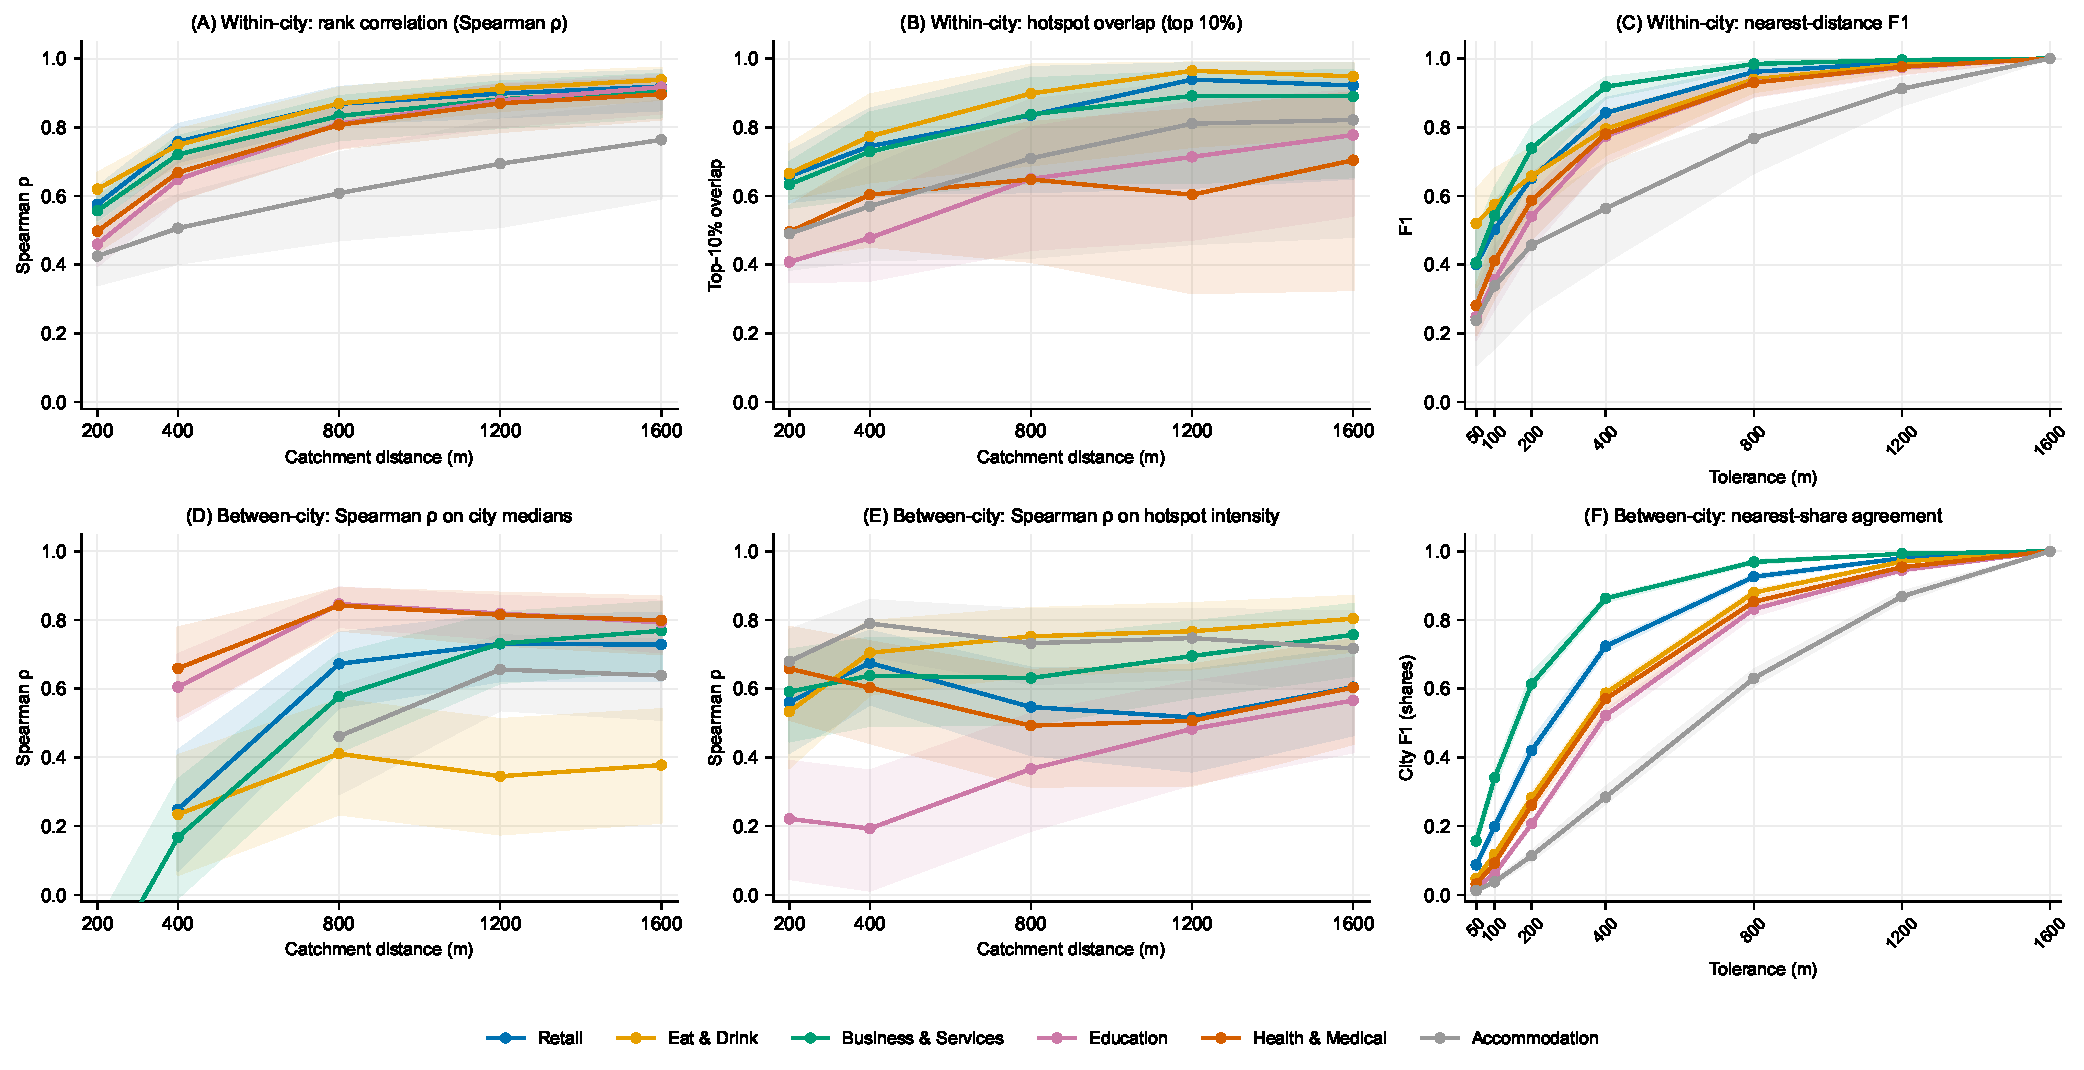
\includegraphics[width=\textwidth]{outputs/figures/fig_pointa_agreement_panels.pdf}
  \caption{\textbf{POI source-substitution agreement by category, task, and spatial scale.}
    \NRefCities{} reference cities. Top row (within-city): (A)~rank correlation (Spearman $\rho$), (B)~hotspot overlap, and (C)~nearest-within-tolerance F1; shaded bands show 95\% spatial block bootstrap CIs (distance-adaptive blocks, $B=200$). Bottom row (between-city): (D)~Spearman $\rho$ on city-level median counts, (E)~Spearman $\rho$ on city-level hotspot intensity, and (F)~harmonic-mean agreement of city-level nearest shares; shaded bands show 95\% city-level bootstrap CIs ($B=2{,}000$).
  }
  \label{fig:pointa_agreement_panels}
\end{figure}

\subsection{Per-city variability}
\label{sec:poi-supp-city-variability}

The main-text figures report median agreement across reference cities. Figure~\ref{fig:pointa_city_variability} shows the underlying per-city distributions at two representative catchment distances (400\,m and 800\,m). The strip plots confirm that the medians are not driven by a small number of outlier cities: at 800\,m most categories have tight distributions for rank correlation, with the bulk of cities exceeding 80\% concordance. Accommodation and Health \& Medical remain consistently the weakest categories with the widest spreads. Figure~\ref{fig:pointa_cross_city_scatter} complements this by plotting city-level median accessibility (log-transformed counts) from Overture against registry values at 800\,m; points falling below the identity line indicate systematic undercounting by Overture, particularly for Retail and Eat \& Drink.

\begin{figure}[p]
  \centering
  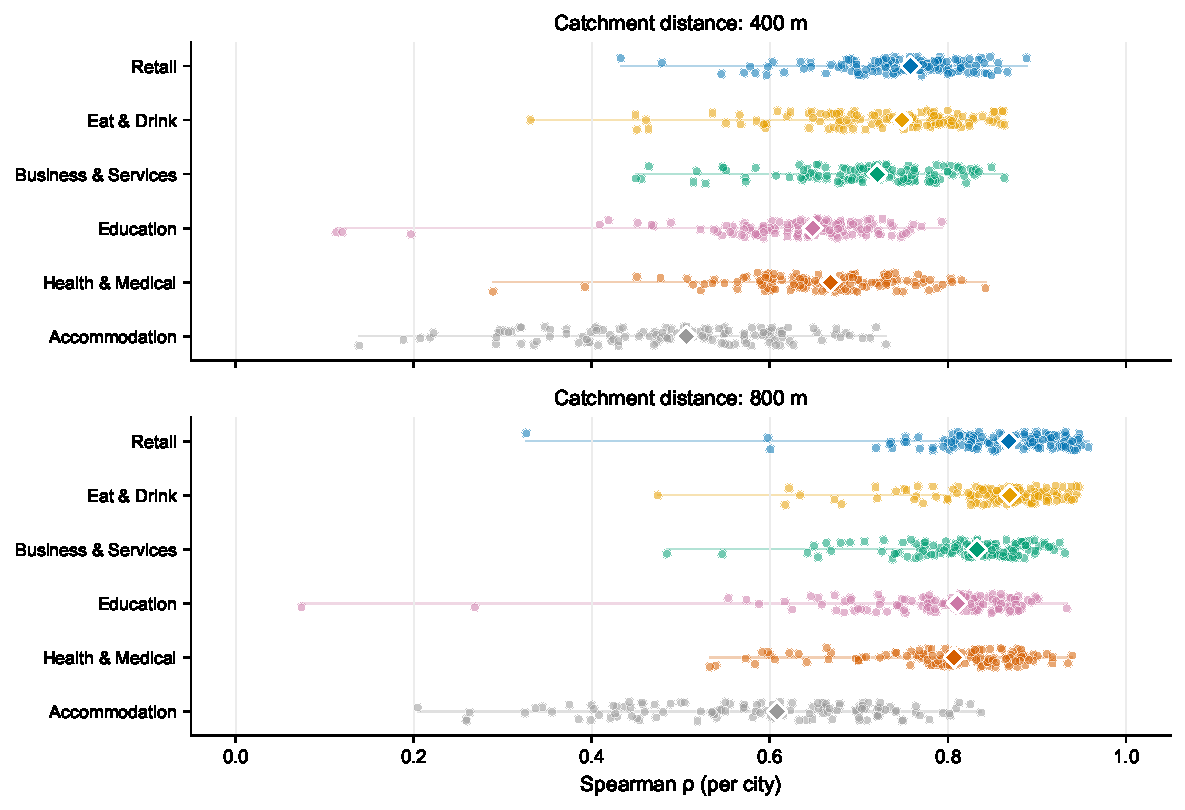
\includegraphics[width=0.88\textwidth]{outputs/figures/fig_pointa_city_variability.pdf}
  \caption{\textbf{Per-city rank correlation spread.}
    Distribution of Spearman $\rho$ (segment-level unweighted counts) across \NRefCities{} reference cities at 400\,m and 800\,m catchments. Points show individual cities; diamonds mark medians.
  }
  \label{fig:pointa_city_variability}

  \vspace{0.5em}

  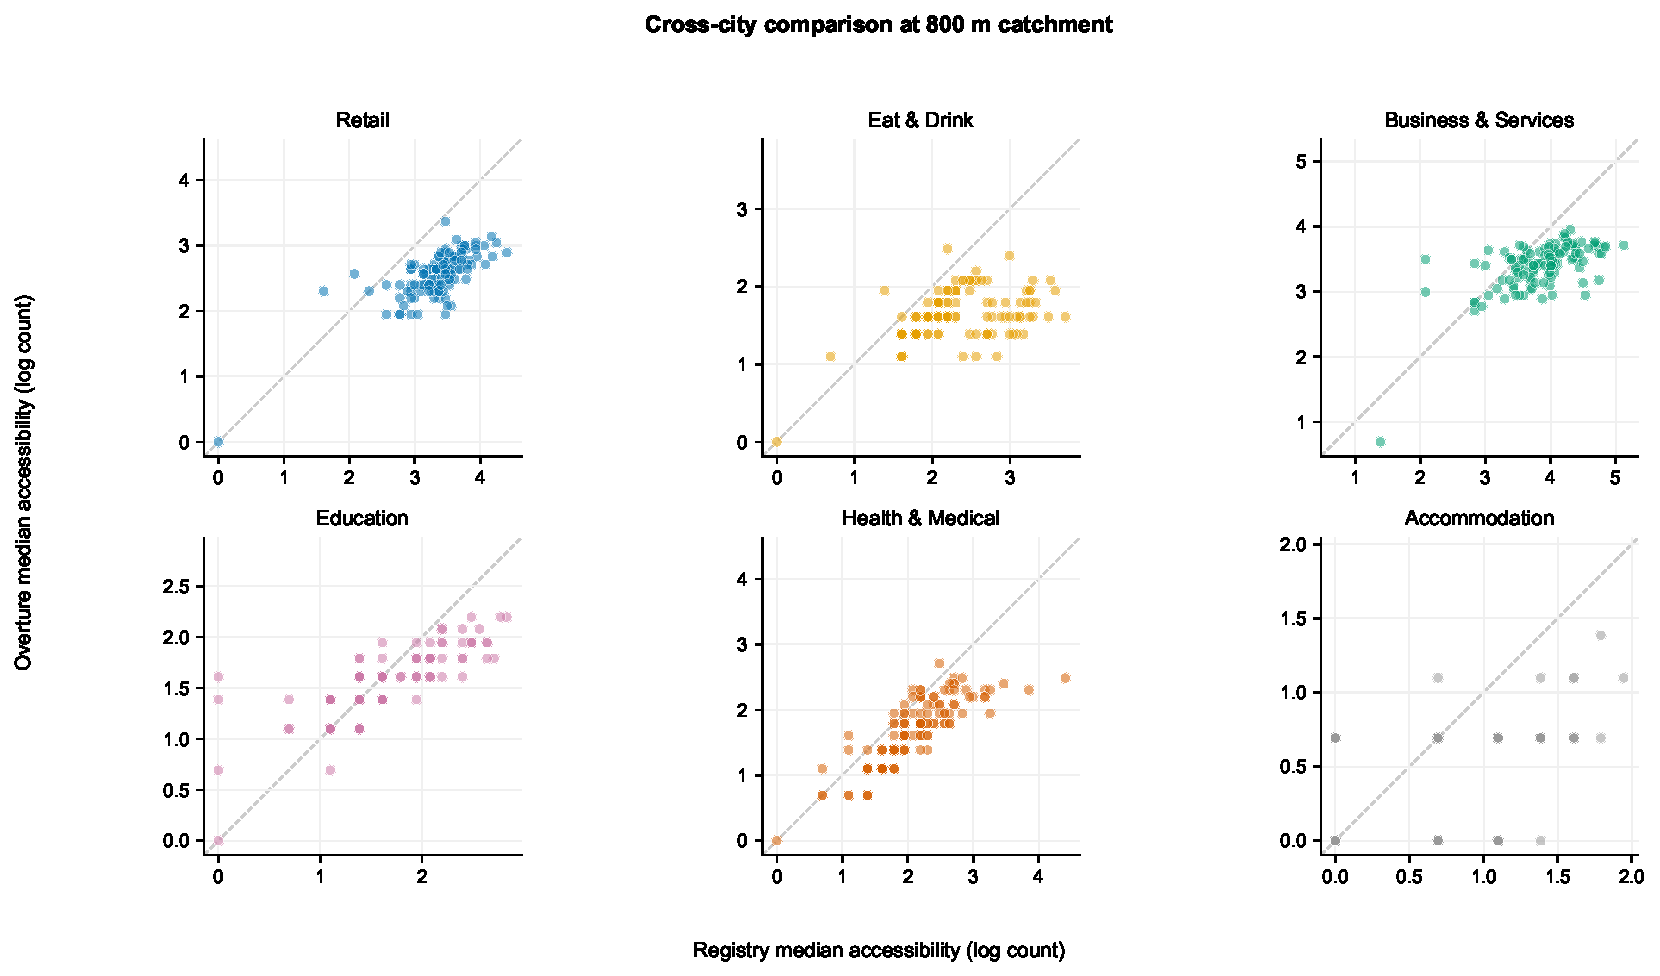
\includegraphics[width=0.88\textwidth]{outputs/figures/fig_pointa_cross_city_scatter.pdf}
  \captionof{figure}{\textbf{Cross-city comparison at 800\,m catchment.}
    Each point is one reference city. Axes show median log-transformed POI counts from registry and Overture sources; the dashed line marks identity. The predominance of points below the line indicates systematic undercounting by Overture, especially for Retail and Eat \& Drink.
  }
  \label{fig:pointa_cross_city_scatter}
\end{figure}

\subsection{Distance-weighted accessibility}
\label{sec:poi-supp-weighted}

The main-text results use unweighted POI counts (the number of establishments reachable within each catchment distance). An alternative is distance-weighted counts, where each POI's contribution decays with network distance, giving greater weight to nearer establishments.

At the same catchment distance, weighted counts produce lower concordance than unweighted counts (typically 3--5 percentage points for rank correlation, 5--8 for hotspot overlap), because the gravity weighting amplifies the effect of small geocoding offsets between sources. However, the weighted measure at 800\,m still exceeds the unweighted measure at 400\,m across all categories, since the larger catchment more than compensates for the concordance lost to weighting. This is relevant for applications that prefer distance-weighted accessibility: reliable concordance is achievable at 800\,m or above. The nearest-distance columns are unchanged, as they do not involve count aggregation.

\clearpage
\section{Building Footprint Source Composition and Metric Sensitivity}
\label{sec:bldg-supp}

This supplement documents the provenance composition of the Overture Maps building footprints used in SOAR-EU and quantifies its effect on derived morphometric indicators.

\subsection{Source classification}
\label{sec:bldg-supp-classification}

Each Overture building footprint carries a \texttt{sources} JSON array whose first element identifies the contributing dataset. We classify these into two groups: \emph{community-contributed} (OpenStreetMap, Esri Community Maps, national cadastral agencies) and \emph{ML-derived} (Microsoft ML Buildings, Google Open Buildings). Community-contributed footprints are digitised or imported from authoritative cadastral sources and generally preserve individual building boundaries; ML-derived footprints are segmented from satellite imagery and may merge adjacent buildings into single polygons or introduce unintended gaps between genuinely attached structures.

Across the \NCitiesTotal{} cities, the footprints draw on several source datasets: OpenStreetMap (dominant in most European cities), Esri Community Maps, Microsoft ML Buildings, and, in Spain, the Instituto Geogr\'{a}fico Nacional cadastre. Country-level aggregates reveal a clear geographic gradient (Table~\ref{tab:building_source_country}; Figure~\ref{fig:building_source_map}): the Netherlands, France, Switzerland, and Belgium are dominated by community sources, while Romania, Spain, Greece, and Bulgaria rely substantially on ML-derived footprints. The per-city ML fraction (Min and Max columns of Table~\ref{tab:building_source_country}) spans from zero in several cadastral-import cities to a large majority in the most ML-reliant. Per-city counts by dataset and country-level summaries are provided in the accompanying CSV files.

\begin{table}[!htb]
  \centering
  \caption{Building footprint source composition by country, sorted by ML-derived fraction (ascending). ML~(\%) is the proportion of footprints from ML-derived sources (primarily Microsoft ML Buildings); Min and Max show the per-city range within each country.}
  \label{tab:building_source_country}
  \scriptsize
  \begin{tabular}{@{}lrrrrr@{}}
  \toprule
  \textbf{Country} & \textbf{Cities} & \textbf{Buildings} & \textbf{ML (\%)} & \textbf{Min (\%)} & \textbf{Max (\%)} \\
  \midrule
  Netherlands & 43 & 6,209,242 & 1.6 & 0.0 & 20.6 \\
  Switzerland & 17 & 794,674 & 4.1 & 0.0 & 11.6 \\
  Luxembourg & 1 & 40,614 & 4.4 & 4.4 & 4.4 \\
  France & 73 & 10,245,743 & 4.5 & 0.0 & 15.2 \\
  Belgium & 16 & 2,627,084 & 5.2 & 1.0 & 16.2 \\
  Ireland & 5 & 769,998 & 5.4 & 3.3 & 8.4 \\
  Norway & 7 & 606,824 & 6.6 & 4.8 & 10.1 \\
  Finland & 6 & 367,553 & 7.8 & 6.2 & 13.5 \\
  Austria & 8 & 688,439 & 8.1 & 4.6 & 18.4 \\
  Denmark & 5 & 647,562 & 8.4 & 5.7 & 9.4 \\
  Estonia & 2 & 102,363 & 8.5 & 6.1 & 13.5 \\
  Germany & 99 & 11,601,375 & 8.8 & 0.1 & 35.7 \\
  Slovakia & 7 & 303,986 & 13.9 & 10.6 & 19.4 \\
  Slovenia & 2 & 98,624 & 15.3 & 13.4 & 19.0 \\
  Lithuania & 4 & 228,098 & 15.7 & 7.8 & 27.1 \\
  Latvia & 2 & 180,865 & 16.1 & 15.8 & 16.7 \\
  Czechia & 12 & 763,959 & 16.7 & 11.6 & 22.1 \\
  Italy & 88 & 4,246,128 & 17.4 & 3.0 & 81.0 \\
  Sweden & 17 & 793,793 & 18.5 & 0.7 & 50.7 \\
  Poland & 63 & 3,612,250 & 18.6 & 4.8 & 37.1 \\
  Croatia & 5 & 272,798 & 24.6 & 16.6 & 33.8 \\
  Hungary & 13 & 944,965 & 27.3 & 16.8 & 61.3 \\
  Portugal & 8 & 916,488 & 27.6 & 18.5 & 57.3 \\
  Bulgaria & 6 & 290,571 & 30.8 & 23.8 & 46.9 \\
  Greece & 8 & 871,146 & 31.3 & 7.5 & 94.9 \\
  Spain & 79 & 3,363,448 & 46.3 & 4.7 & 94.9 \\
  Romania & 29 & 1,319,339 & 48.0 & 23.6 & 86.1 \\
  Malta & 1 & 49,893 & 54.8 & 54.8 & 54.8 \\
  \bottomrule
\end{tabular}
\end{table}

\begin{figure}[!htb]
  \centering
  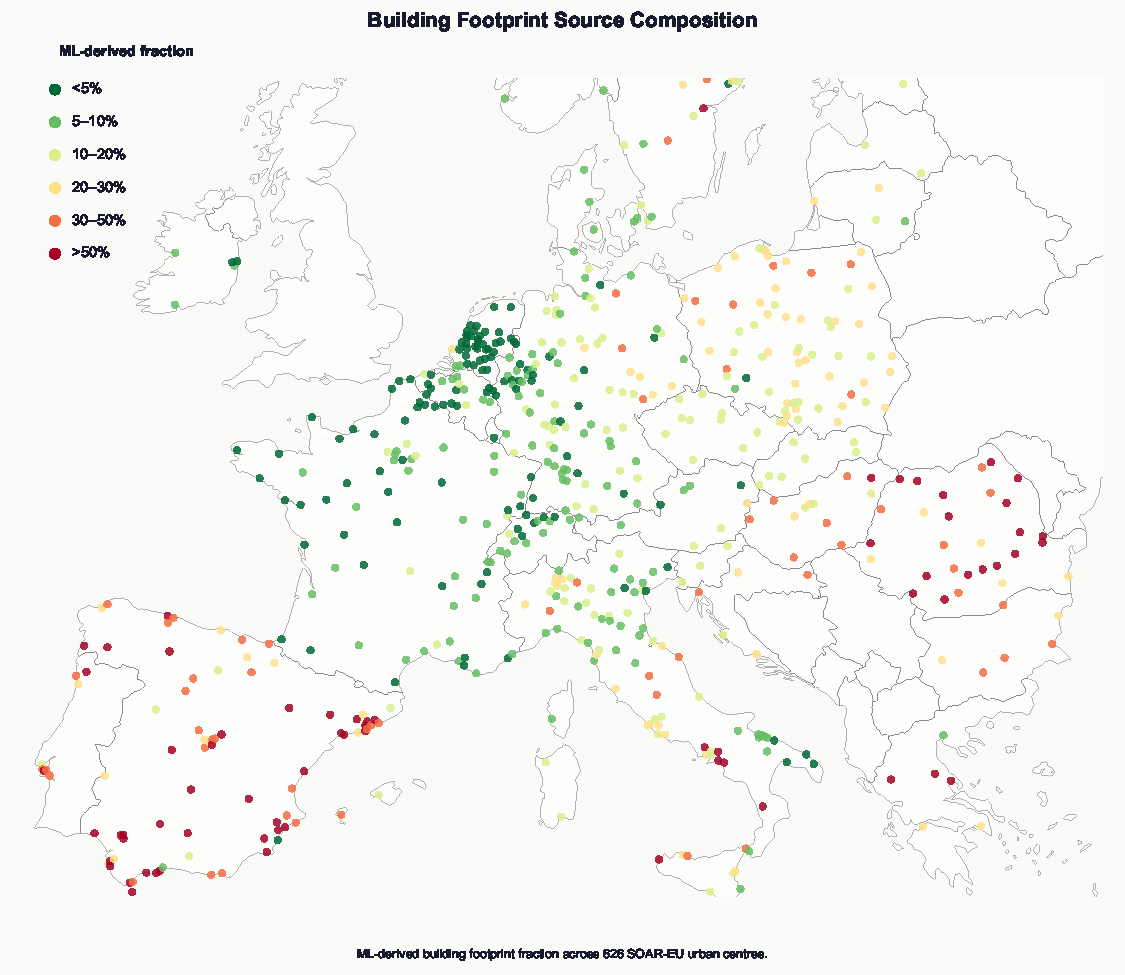
\includegraphics[width=\textwidth]{outputs/figures/fig_building_source_map.pdf}
  \caption{ML-derived building footprint fraction across the \NCitiesTotal{} SOAR-EU urban centres. Cities in western and northern Europe (France, Netherlands, Belgium, Germany) are dominated by community-contributed sources; cities in southern and eastern Europe (Romania, Spain, Greece, Bulgaria) rely more heavily on ML-derived footprints.}
  \label{fig:building_source_map}
\end{figure}

\subsection{Effect on morphometric indicators}
\label{sec:bldg-supp-sensitivity}

We test for source-driven bias at two levels.

\paragraph{Cross-city correlations.} For each morphometric indicator, we compute the Spearman correlation between each city's ML fraction and its median metric value across the \NCitiesTotal{} cities (Table~\ref{tab:building_metric_sensitivity}). Shared wall ratio shows the strongest negative association: cities with more ML-derived buildings have lower shared wall ratios. This cross-city correlation conflates two effects: a genuine morphological gradient (countries with higher ML fractions---Romania, Bulgaria, Greece---also have more freestanding housing stock) and a data artefact (ML-derived footprints underestimate shared walls due to polygon boundary gaps). The within-city test below isolates the artefact component. Perimeter, area, and volume are also positively associated, partly reflecting the tendency of ML segmentation to merge adjacent buildings into larger polygons and partly reflecting genuinely larger building footprints in lower-density settings. Fractal dimension and corner count show weaker but significant associations, while compactness, shape index, and orientation show no significant association with source composition.

\paragraph{Within-city comparisons.} To isolate the data artefact from genuine morphological differences between countries, we compare community and ML-derived buildings \emph{within the same city} using Mann-Whitney $U$ tests, restricted to cities containing both source types (Table~\ref{tab:building_metric_sensitivity}). Shared wall ratio shows a consistent within-city difference, significant in nearly all such cities: ML-derived buildings have lower shared wall ratios than community-contributed buildings in the same urban context, confirming a per-building artefact independent of cross-country morphological variation. Corner count and fractal dimension are also affected within cities, while compactness and shape index show small but widespread differences.

Block-level density metrics (GSI, FSI) show no meaningful cross-city association with ML fraction, likely because ML footprints add buildings in areas where community mapping is sparse, compensating for any area inflation from polygon merging. Table~\ref{tab:building_metric_sensitivity} summarises all cross-city and within-city results.

\begin{table}[!htb]
  \centering
  \caption{Sensitivity of building morphometric indicators to data source composition. Cross-city $\rho$: Spearman correlation between city ML fraction and city median metric value, across all \NCitiesTotal{} cities. Within-city $r$: median rank-biserial correlation from Mann-Whitney $U$ tests comparing community and ML-derived buildings within each city, restricted to cities containing both source types. Significance: {*}{*}{*}\,$p < 0.001$, {*}{*}\,$p < 0.01$, {*}\,$p < 0.05$.}
  \label{tab:building_metric_sensitivity}
  \scriptsize
  \begin{tabular}{@{}lrrrl@{}}
  \toprule
  \textbf{Metric} & \textbf{Cross-city $\rho$} & \textbf{$p$} & \textbf{Within-city $r$} & \textbf{Sig.} \\
  \midrule
  Perimeter & +0.534 & $<$0.001 & --- & *** \\
  Shared Wall Ratio & -0.515 & $<$0.001 & -0.36 & *** \\
  Area & +0.513 & $<$0.001 & --- & *** \\
  Volume & +0.508 & $<$0.001 & --- & *** \\
  Shared Walls & -0.437 & $<$0.001 & --- & *** \\
  Block FSI & +0.372 & $<$0.001 & --- & *** \\
  Form Factor & -0.217 & $<$0.001 & --- & *** \\
  Fractal Dimension & -0.196 & $<$0.001 & -0.12 & *** \\
  Frontage Max & -0.178 & $<$0.001 & --- & *** \\
  Block GSI & +0.111 & 0.006 & --- & ** \\
  Corners & +0.098 & 0.015 & -0.26 & * \\
  Mean Height & +0.098 & 0.016 & --- & * \\
  Orientation & -0.060 & 0.136 & --- &  \\
  Compactness & +0.055 & 0.171 & +0.13 &  \\
  Shape Index & +0.055 & 0.171 & +0.13 &  \\
  \bottomrule
\end{tabular}
\end{table}

\subsection{Street-frontage ratio}
\label{sec:bldg-supp-frontage}

To provide a source-robust continuity measure, we compute a bilateral street-frontage ratio for each street segment. The computation proceeds as follows: (1)~buffer the street centreline by 35\,m to define a corridor (wide enough to capture building edges that address the street across a typical European front-garden or setback depth, narrow enough to exclude buildings on the next parallel street); (2)~identify all building edges whose midpoint falls inside the corridor and whose nearest street is this one (preventing cross-street contamination); (3)~classify each edge as left or right of the centreline using the local street tangent; (4)~per side, retain only edges within 5\,m of the closest edge, filtering out rear extensions and garages while preserving the primary facade line (5\,m is chosen to span typical facade step-ins and arcades without admitting rear-yard structures); (5)~project retained edges onto the centreline, merge overlapping intervals, and compute coverage as the fraction of street length covered (3\,m trimmed from each end as a junction guard, removing the short overlap where a corner property's facade would otherwise count toward both intersecting streets); (6)~the reported score (\texttt{frontage\_max}) is the maximum of the two sides. Per-side scores (\texttt{frontage\_left}, \texttt{frontage\_right}), their mean (\texttt{frontage\_avg}), and per-side edge counts (\texttt{frontage\_edges\_left}, \texttt{frontage\_edges\_right}) are also retained.

Unlike shared wall ratio, which requires exact topological contact between adjacent polygon boundaries, frontage ratio depends only on building \emph{presence} along the street edge. Whether two adjacent terraced houses are represented as separate touching polygons (community-digitised) or as a single merged polygon (ML-derived), the frontage coverage is the same. Across the \NCitiesTotal{} cities, the association between city-level ML fraction and median frontage ratio is substantially weaker than the corresponding shared-wall-ratio association (Table~\ref{tab:building_metric_sensitivity}). Because frontage is largely immune to the polygon-merging artefact that the within-city test identifies for shared wall ratio, this weaker residual association most likely reflects a predominantly genuine morphological gradient (countries with higher ML fractions also tend toward more freestanding housing) rather than a measurement artefact.

\end{document}
'
%
% If you hit a cryptic build error after edits (e.g., "Runaway argument" while
% writing labels/outlines), remove auxiliary files and rebuild:
%   rm -f manuscript.aux manuscript.out manuscript.toc manuscript.bbl manuscript.blg
%   pdflatex manuscript.tex && pdflatex manuscript.tex
\providecommand{\preprintmode}{0}
\newcommand{\IfPreprintTF}[2]{\ifnum\preprintmode=1\relax #1\else #2\fi}
\newcommand{\SpecsTableHeading}{\IfPreprintTF{Dataset summary}{Specifications Table}}
\newcommand{\ValueHeading}{\IfPreprintTF{Value of the dataset}{Value of the Data}}

% Submission placeholders (override at build time if desired)
\providecommand{\ZenodoDoi}{10.5281/zenodo.18961227}
\providecommand{\ZenodoUrl}{https://doi.org/10.5281/zenodo.18961227}
\providecommand{\GrantNumber}{101078890}

\usepackage[utf8]{inputenc}
\usepackage[margin=2.5cm]{geometry}
\usepackage{graphicx}
\usepackage{booktabs}
\PassOptionsToPackage{hyphens}{url}\usepackage{hyperref}
\usepackage{siunitx}
\usepackage{xcolor}
\usepackage{longtable}
\usepackage{multirow}
\usepackage{array}
\usepackage{float}        % Better float positioning
\usepackage{placeins}     % \FloatBarrier command
\usepackage{enumitem}     % Better list formatting
\usepackage{caption}      % \captionof for multi-figure floats
\usepackage{wrapfig}      % text-wrapping figures
\usepackage{amssymb}      % For \checkmark symbol
\usepackage{pdflscape}    % For landscape pages in supplementary

% Avoid hyperref warnings from elsarticle author-note macros in PDF strings
% (e.g., when writing metadata/bookmarks).
\makeatletter
\pdfstringdefDisableCommands{%
  \def\corref#1{}%
  \def\cnotenum{}%
  \def\@corref#1{}%
}
\makeatother

% Allow line breaks after underscores so long \texttt{} filenames
% (e.g. building\_source\_counts.csv) can wrap instead of overrunning the margin.
\renewcommand{\_}{\textunderscore\allowbreak}

% Auto-generated statistics macros (from paper_stats.json)
% Auto-generated LaTeX macros
% Generated by: python paper_data/code/s06_write_paper_macros.py
% DO NOT EDIT MANUALLY - regenerate from source data
% === City Counts ===
\newcommand{\NCitiesTotal}{626}
\newcommand{\NCountries}{28}
\newcommand{\NRefCities}{116}
\newcommand{\NRefCitiesFr}{73}
\newcommand{\NRefCitiesNl}{43}
\newcommand{\NNonRefCities}{510}

% === Data Coverage ===
\newcommand{\NCitiesLowHeight}{94}
\newcommand{\NCitiesNoHeight}{20}
\newcommand{\NCitiesWithHeightsRaster}{611}
\newcommand{\BldgHeightsAgeYears}{14}
\newcommand{\MedianHeightCoverage}{71}
\newcommand{\MedianBlockHundredCoverage}{74}
\newcommand{\NCitiesNoBlocks}{24}
\newcommand{\NCitiesNoEmployment}{185}

% === Dataset Size ===
\newcommand{\DatasetTotalCompressedGB}{35}
\newcommand{\DatasetMinMB}{3.5}
\newcommand{\DatasetMaxGB}{1.2}
\newcommand{\DatasetMeanMB}{56}

% === POI Validation Thresholds ===
\newcommand{\PoiNearDistGoodM}{800}
\newcommand{\PoiNearDistOtherM}{800}
\newcommand{\PoiNearDistAccomM}{1200}

% === Displacement Stats ===


% Consistent table column types
\newcolumntype{L}[1]{>{\raggedright\arraybackslash}p{#1}}
\newcolumntype{C}[1]{>{\centering\arraybackslash}p{#1}}
\newcolumntype{R}[1]{>{\raggedleft\arraybackslash}p{#1}}

\IfPreprintTF{}{\journal{Data in Brief}}

\begin{document}

\begin{frontmatter}

  \title{SOAR-EU: A Scalable, Open, Automatable, and Reproducible European Urban Dataset}

  \author[spacesyntax]{Gareth Simons\corref{cor1}}
  \ead{gareth.simons@ucl.ac.uk}
  \cortext[cor1]{Corresponding author}

  \author[spacesyntax]{Kayvan Karimi}
  \author[spacesyntax]{Sepehr Zhand}

  \affiliation[spacesyntax]{organization={Space Syntax Laboratory, UCL Bartlett School of Architecture},
    addressline={22 Gordon Street},
    city={London},
    country={United Kingdom}
  }

  \begin{abstract}
    Constructing spatial analytic datasets, particularly at scale, remains resource-intensive; SOAR-EU (Scalable, Open, Automatable, Reproducible --- European Urban) addresses this by providing ready-to-use pedestrian-scale urban metrics for \NCitiesTotal{} European cities across \NCountries{} countries to support comparative urban analytic research at the continental scale. Integrating GHS-UCDB urban boundaries, Eurostat census data, Copernicus Urban Atlas, and Overture Maps, it delivers over 100 pre-computed metrics per street at multiple spatial scales, covering network centrality, land-use and infrastructure accessibility, mixed-use diversity, building and block morphology, green-space and tree-canopy proximity, and demographics. Processing is automatable via open-source Python with fixed parameters; data are distributed as GeoPackage files in EPSG:3035. Because the Overture Maps POI layer aggregates commercial and editorial sources of varying completeness, we evaluate POI-derived accessibility through source-substitution replication against independent registries in \NRefCities{} reference cities in France and the Netherlands, providing task- and scale-specific guidance on when these metrics are more or less suitable for within-city pattern analysis and for broad between-city comparison.
  \end{abstract}

  \begin{keyword}
    pedestrian accessibility \sep
    street networks \sep
    land-use diversity \sep
    building morphology \sep
    walkability \sep
    cross-city comparison \sep
    spatial metrics
  \end{keyword}

\end{frontmatter}

%% ============================================================================
%% SPECIFICATIONS TABLE
%% ============================================================================
\section*{\SpecsTableHeading}

\begin{table}[!htbp]
  \centering
  \small
  \begin{tabular}{@{}L{3.2cm}L{8.3cm}@{}}
    \toprule
    \textbf{Subject} & Geography, Urban Studies, Geospatial Data Science \\
    \midrule
    \textbf{Specific subject area} & Urban morphology, pedestrian accessibility, land-use diversity \\
    \midrule
    \textbf{Type of data} & Table (geospatial vector); Processed, filtered (GeoPackage format) \\
    \midrule
    \textbf{Data format} & GeoPackage (.gpkg); one ZIP archive per country bundling the city GeoPackages, plus a boundary index file \\
    \midrule
    \textbf{How data was acquired} & Programmatic extraction and processing of open geospatial sources using Python (cityseer, momepy, GeoPandas). Metrics computed on natural street segments at multiple distance thresholds \\
    \midrule
    \textbf{Data collection} & Derived from publicly available authoritative sources: GHS-UCDB R2024A (2025 reference epoch), Overture Maps Foundation (2026 release), Copernicus Urban Atlas (2021), Copernicus Street Tree Layer (2021), Copernicus Height Model (2012), Eurostat Census Grid (2021) \\
    \midrule
    \textbf{Parameters for data collection} & Centrality thresholds: 400--9,600\,m. Accessibility thresholds: 200--1,600\,m. Morphology thresholds: 200--400\,m. CRS: EPSG:3035. See \href{https://github.com/UCL/t2e-soar-eu}{repository} for full configuration \\
    \midrule
    \textbf{Data source location} & Pan-European: \NCitiesTotal{} urban centres across 26 EU member states plus Norway and Switzerland (Liechtenstein has no qualifying urban centre under the GHS-UCDB threshold, and Cyprus is not covered by the GHS-UCDB R2024A European regional file used here). Coordinate Reference System: EPSG:3035 (ETRS89-LAEA Europe) \\
    \midrule
    \textbf{Data accessibility} & Repository: Zenodo. Data identification number: \ZenodoDoi{}. URL: \ZenodoUrl{} \\
    \midrule
    \textbf{Related research article} & G.\ Simons, K.\ Karimi, S.\ Zhand, A Morphological Atlas of European Urbanism: Eight Types of Urban Fabric Across Six Hundred Cities (SOAR-EU), submitted to \textit{Computers, Environment and Urban Systems}. \\
    \bottomrule
  \end{tabular}
\end{table}

%% ============================================================================
%% VALUE OF THE DATA
%% ============================================================================
\section*{\ValueHeading}

\begin{itemize}[leftmargin=*]
  \item The dataset enables \textbf{consistent comparative research} by removing the methodological confounds that usually frustrate cross-city work: all \NCitiesTotal{} cities are processed with identical methods, parameters, and source datasets, so measured differences reflect the urban fabric rather than differing analytical choices or bespoke data pipelines. This shared baseline supports benchmarking against continental norms, clustering streets into urban typologies, and detecting systematic differences in walkability and land use. Comparability is nonetheless bounded by the geographic consistency of the underlying open sources (Section~\ref{sec:provenance}): broad distributional comparison across regions and city groups is more strongly supported than exact city-by-city ranking, particularly for POI-derived metrics outside the validated French and Dutch reference set.
  \item The \textbf{multi-scale design} supports sensitivity analysis and scale-appropriate interpretation. Centrality metrics span 400\,m to 9,600\,m (5--120 minute walking catchments); accessibility metrics span 200\,m to 1,600\,m. Because relationships observed at one scale may not hold at others \cite{openshaw1984}, multiple thresholds are provided.
  \item The dataset supports \textbf{network-based accessibility} analysis that follows pedestrian routes rather than Euclidean buffers \cite{apparicio2008}. A park 200\,m as-the-crow-flies but 800\,m by foot is treated as 800\,m away. For each land-use category, both unweighted and distance-weighted counts are provided, supporting more nuanced aggregations in which proximity can be weighted by distance impedance.
  \item Researchers can benefit from the \textbf{fine-grained resolution} at street-segment level, which preserves within-neighbourhood heterogeneity and supports analysis from individual streets to city-wide patterns.
  \item The pipeline supports \textbf{reproducibility}: processing code and parameter settings are documented, enabling researchers to verify, regenerate, or extend the dataset as sources improve.
  \item The dataset benefits \textbf{urban planners, transport researchers, public health scientists, and environmental analysts} who need comparable pedestrian-scale indicators across European cities but lack the resources to assemble multi-source geospatial pipelines from scratch.
\end{itemize}

%% ============================================================================
%% OBJECTIVE
%% ============================================================================
\section*{Objective}

Comparative urban research requires consistent measurement across cities, yet constructing spatial analytic datasets remains resource-intensive. Related work includes GHSL \cite{pesaresi2023} global built-up surface mapping, Boeing's \cite{boeing2020} analysis of US street networks, Fleischmann et al.'s \cite{fleischmann2022} numerical taxonomy of urban form, and Yap and Biljecki's \cite{yap2023} feature-rich network dataset for 50 cities. Simons's \cite{simons2021thesis} pedestrian-scale integration of street networks, land use, and census demographics across 931 cities and towns in Great Britain is a direct methodological precursor to the present continental-scale dataset.

SOAR-EU (Scalable, Open, Automatable, Reproducible --- European Urban) complements these by providing ready-to-use pedestrian-scale metrics for \NCitiesTotal{} EU urban centres. The dataset integrates GHS-UCDB boundaries, Eurostat census grids, Copernicus land cover and building heights, and Overture Maps street networks and POIs. Metrics are computed on street segments across multiple spatial scales (200--9,600\,m) using the cityseer \cite{simons2023} Python package, spanning network centrality, land-use and infrastructure accessibility, mixed-use diversity, building and block morphology, green-space and tree-canopy proximity, and demographics. The pipeline is open-source and designed for regeneration as future data releases become available.

%% ============================================================================
%% DATA DESCRIPTION
%% ============================================================================
\section{Data Description}

\subsection{Dataset Structure}
\label{sec:dataset-structure}

The dataset comprises a \texttt{boundaries.gpkg} file derived from the GHS-UCDB urban centre boundaries, plus \NCountries{} country-level ZIP archives (\texttt{soar\_eu\_\{country\}.zip}) that bundle the \NCitiesTotal{} individually compressed city GeoPackages. Each city file follows the naming convention \texttt{metrics\_\{bounds\_fid\}.gpkg.zip}, where \texttt{bounds\_fid} corresponds to the unique identifier from \texttt{boundaries.gpkg}.

Each GeoPackage contains three layers: \textbf{streets} (natural street segments with computed metrics as LineString geometries), \textbf{buildings} (individual footprints with morphological attributes), and \textbf{blocks} (urban blocks with source and morphological attributes). The streets layer contains only \emph{live} segments (those whose midpoint falls within the urban centre boundary), excluding peripheral buffer segments used solely for edge-effect mitigation during network and accessibility analysis. Individual city files range from approximately \DatasetMinMB\,MB to \DatasetMaxGB\,GB depending on urban extent (average $\sim$\DatasetMeanMB\,MB); the complete compressed dataset is approximately \DatasetTotalCompressedGB\,GB. End-to-end processing takes approximately one day on a contemporary workstation-class laptop (18-core Apple M5 Pro).

Per-column completeness and building-source composition tables (\texttt{completeness\_coverage.csv}, \texttt{building\_source\_counts.csv}, and \texttt{building\_source\_by\_country.csv}) are bundled with the deposit; coverage is summarised in Section~\ref{sec:coverage} and source composition is interpreted in Section~\ref{sec:provenance}.

\subsection{Streets Layer}

The streets layer is the core of the dataset: each live segment carries pre-computed metrics spanning the full set of measure families: network centrality, land-use accessibility and mixed-use diversity, infrastructure accessibility, building and block morphology, green-space and tree-canopy proximity, and interpolated census demographics. Most are computed at several network-distance thresholds, indicated by a suffix (e.g., \texttt{\_400}, \texttt{\_800}). Table~\ref{tab:streets_schema} summarises the attribute groups; the complete per-column schema is given in Supplementary Material (Section~S1).

\begin{table}[!htbp]
  \centering
  \caption{Summary of streets layer attributes (selected metrics shown; full schema in Supplementary Material Section~S1).}
  \label{tab:streets_schema}
  \small
  \begin{tabular}{@{}L{4cm}L{8.1cm}@{}}
    \toprule
    \textbf{Attribute group} & \textbf{Description} \\
    \midrule
    \texttt{geometry}, \texttt{x}, \texttt{y} & Segment geometry and midpoint coordinates (EPSG:3035) \\
    \midrule
    \texttt{cc\_beta\_*} & Closeness centrality (gravity-weighted) at distance thresholds \\
    \midrule
    \texttt{cc\_harmonic\_*} & Harmonic closeness centrality \\
    \midrule
    \texttt{cc\_hillier\_*} & Hillier-type closeness (node count / mean distance) \\
    \midrule
    \texttt{cc\_farness\_*} & Farness (total network distance to reachable segments) \\
    \midrule
    \texttt{cc\_betweenness\_*} & Segment betweenness centrality \\
    \midrule
    \texttt{cc\_betweenness\_beta\_*} & Beta-weighted betweenness centrality \\
    \midrule
    \texttt{cc\_density\_*} & Street segment density within threshold \\
    \midrule
    \texttt{cc\_cycles\_*} & Network cycle count within threshold \\
    \midrule
    \texttt{cc\_\{landuse\}\_*\_nw} & Unweighted POI count for land-use category \\
    \midrule
    \texttt{cc\_\{landuse\}\_*\_wt} & Distance-weighted POI count for land-use category \\
    \midrule
    \texttt{cc\_\{landuse\}\_nearest\_max\_*} & Distance to nearest POI in category \\
    \midrule
    \texttt{cc\_\{infra\}\_*\_nw/wt} & Infrastructure accessibility: transport, parking, street-furniture counts \\
    \midrule
    \texttt{cc\_hill\_*} & Land-use diversity (Hill numbers $q=0,1,2$) \\
    \midrule
    \texttt{cc\_green\_nearest\_max\_*} & Distance to nearest green space \\
    \midrule
    \texttt{cc\_trees\_nearest\_max\_*} & Distance to nearest tree canopy \\
    \midrule
    \texttt{cc\_green\_area\_sum\_*}, \texttt{cc\_trees\_area\_sum\_*} & Green-space / tree-canopy area within threshold \\
    \midrule
    \texttt{cc\_*\_median\_*} & Building morphology, contextual aggregation (area, height, volume, compactness, shared-wall ratio, \ldots) \\
    \midrule
    \texttt{cc\_building\_*} & Building count within threshold \\
    \midrule
    \texttt{frontage\_max} & Bilateral street-frontage ratio: max(left, right) building coverage (0--1) \\
    \midrule
    \texttt{cc\_block\_*} & Contextual block morphology: area, perimeter, compactness, GSI, FSI, OSR, storeys, height \\
    \midrule
    \texttt{density}, \texttt{t}, \texttt{emp} & Interpolated census demographics (population, density, age, employment, nationality, migration) \\
    \bottomrule
  \end{tabular}
\end{table}

Two of these families, land-use and infrastructure accessibility, count points of interest grouped into analytical categories. The 11 land-use categories (\texttt{cc\_\{landuse\}\_*}) are listed in Table~\ref{tab:landuse} and the three infrastructure categories (\texttt{cc\_\{infra\}\_*}) in Table~\ref{tab:infrastructure}; both derive from Overture's classification as described in Section~\ref{sec:landuse-access}.

\begin{table}[!htbp]
  \centering
  \caption{Aggregated land-use categories derived from Overture Maps POI classification.}
  \label{tab:landuse}
  \small
  \begin{tabular}{@{}L{4.2cm}L{7.8cm}@{}}
    \toprule
    \textbf{Category} & \textbf{Includes} \\
    \midrule
    \texttt{eat\_and\_drink} & Restaurants, cafés, bars \\
    \texttt{retail} & Shops, supermarkets, pharmacies \\
    \texttt{business\_and\_services} & Automotive, beauty/spa, financial, home, professional services, real estate, travel agencies, pets, media, corporate offices \\
    \texttt{public\_services} & Government offices, libraries, civic facilities \\
    \texttt{health\_and\_medical} & Hospitals, doctors, dentists, optometrists \\
    \texttt{education} & Schools, universities, driving schools \\
    \texttt{accommodation} & Hotels, hostels, lodging \\
    \texttt{active\_life} & Sports facilities, fitness centres, recreation \\
    \texttt{arts\_and\_entertainment} & Cinemas, theatres, performance venues \\
    \texttt{attractions\_and\_activities} & Museums, landmarks, tourist attractions \\
    \texttt{religious} & Places of worship \\
    \bottomrule
  \end{tabular}
\end{table}

\begin{table}[!htbp]
  \centering
  \caption{Infrastructure categories derived from Overture Maps infrastructure theme.}
  \label{tab:infrastructure}
  \small
  \begin{tabular}{@{}L{3cm}L{9cm}@{}}
    \toprule
    \textbf{Category} & \textbf{Includes} \\
    \midrule
    \texttt{transport} & Bus stops, bus stations, railway stations, subway stations, ferry terminals, airports (including regional, international, seaplane), aerialway stations, helipads \\
    \texttt{street\_furn} & Benches, drinking water points, fountains, planters, plants, post boxes, picnic tables \\
    \texttt{parking} & Parking lots, motorcycle parking \\
    \bottomrule
  \end{tabular}
\end{table}

\subsection{Buildings and Blocks Layers}

The buildings layer contains individual building footprints derived from Overture Maps with morphological metrics including area, perimeter, compactness, orientation, estimated height (sampled from raster), volume, floor area, form factor, corners, shape index, shared wall ratio, and fractal dimension. Each footprint retains its Overture \texttt{sources} attribute, recording the contributing dataset (e.g., OpenStreetMap, Microsoft ML Buildings). The blocks layer provides urban block geometries derived from Urban Atlas with block-level morphology (area, perimeter, compactness, orientation, computed via the momepy package \cite{fleischmann2019}) and Spacematrix indicators: ground space index (GSI, building coverage ratio), floor space index (FSI), open space ratio (OSR), mean number of storeys (L), and area-weighted mean building height. Block-level morphology is reported only for built-up blocks; very small and oversized blocks are filtered out (appearing as NaN), with the thresholds and rationale given in Section~\ref{sec:metric-computation}.

\subsection{Coverage and Completeness}
\label{sec:coverage}

A per-column completeness report (\texttt{completeness\_coverage.csv}) is included with the dataset, listing the non-null coverage share for every attribute column in each city's streets, buildings, and blocks layers. Building footprint source composition is documented in \texttt{building\_source\_counts.csv} (per-city counts by source dataset) and \texttt{building\_source\_by\_country.csv} (country-level summaries); see Section~\ref{sec:provenance} for interpretation. Most metric groups (centrality, land-use and infrastructure accessibility, diversity, green-space and tree-canopy proximity, and building morphology) have near-complete coverage across all cities. Three categories exhibit variable coverage:

\begin{itemize}[nosep]
  \item \textbf{Height-derived metrics.} Building heights are sampled from the 2012 Copernicus Digital Height Model raster, whose spatial footprint does not cover all cities uniformly. Height-dependent attributes (mean height, volume, form factor, and their street-level contextual summaries) have a median coverage of \MedianHeightCoverage\%, with \NCitiesLowHeight{} cities below 50\% and \NCitiesNoHeight{} cities with no height data at all.\footnote{The \NCitiesNoHeight{}-city figure is derived per-column from \texttt{completeness\_coverage.csv}; it differs from the count of cities for which a Copernicus DHM raster was delivered at all (\NCitiesWithHeightsRaster{}/\NCitiesTotal{}) because some delivered rasters contain no usable pixels inside the city extent.}
  \item \textbf{Block morphology at 200\,m.} Contextual block metrics at the 200\,m threshold (area, perimeter, compactness, orientation, coverage ratio, and Spacematrix indicators) have a median coverage of \MedianBlockHundredCoverage\% (\NCitiesNoBlocks{} cities at zero). Coverage is reported over the filtered \emph{built-up} blocks layer that ships with each city file. Urban Atlas blocks classed as roads, rail, water, wetlands, agriculture, forest, green urban areas, sports/leisure, or otherwise exceeding 2\,km\textsuperscript{2} are excluded from urban morphological metrics (see Section~\ref{sec:metric-computation}), which particularly affects streets near city peripheries. The residual variability reflects a spatial scale effect: some street segments do not have any qualifying block within a 200\,m network radius. The same metrics at the 400\,m threshold have substantially higher coverage.
  \item \textbf{Employment.} Eurostat employment counts (\texttt{emp}, \texttt{emp\_\%}) are unavailable for \NCitiesNoEmployment{} cities, reflecting gaps in the upstream Census Grid. All other demographic variables (population, age structure, gender, nationality, migration) are near-universal.
\end{itemize}

\noindent The coverage report documents per-column coverage for each of these metric groups.

\subsection{Example Output}

Figure~\ref{fig:example-amsterdam} illustrates SOAR-EU output for Amsterdam, showing four representative metrics computed on the street network. Panel (A) shows closeness centrality at 800\,m, capturing network accessibility. Panel (B) shows retail catchment, the count of retail POIs reachable within 400\,m network distance, with higher values concentrated in the historic centre. Panel (C) shows distance to nearest green or blue space, indicating park and water proximity across the urban fabric. Panel (D) shows population density interpolated from the Eurostat Census Grid 2021 (1\,km\textsuperscript{2} resolution), expressed as persons per km\textsuperscript{2} of land surface. All metrics use network-based distances for aggregation, except for census statistics which are interpolated.

\begin{figure}[!htbp]
  \centering
  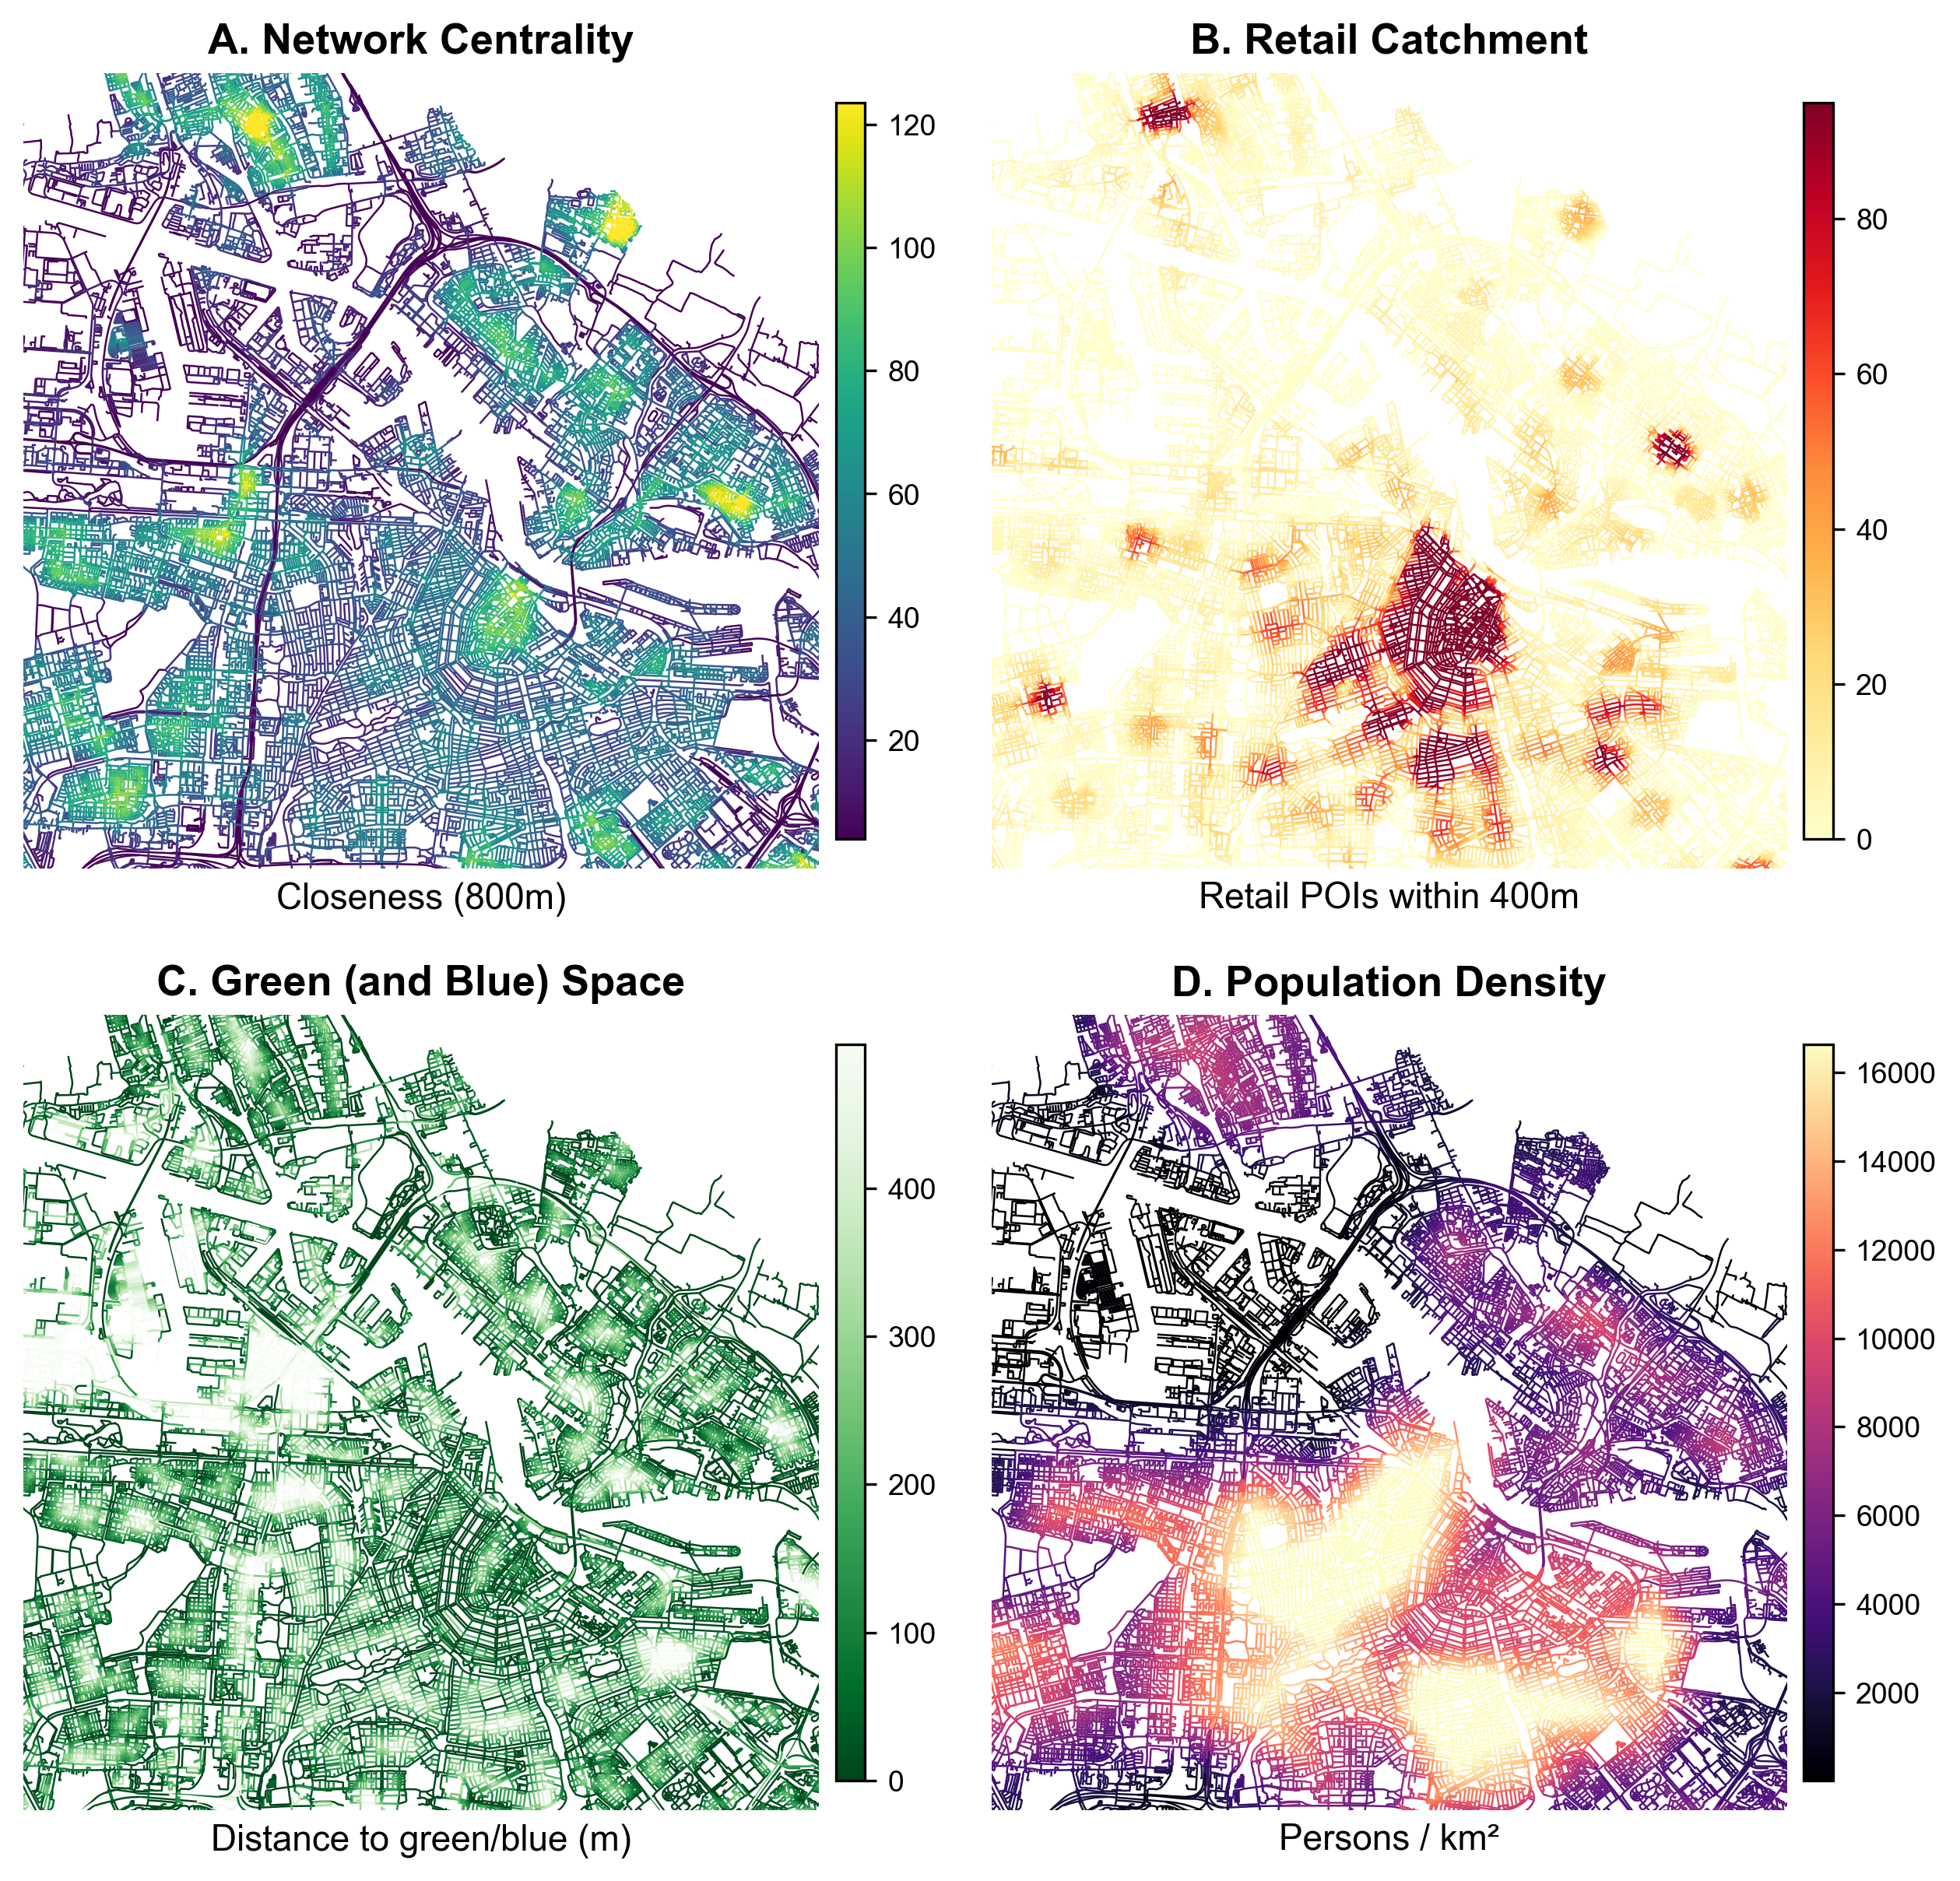
\includegraphics[width=\textwidth]{outputs/figures/fig_example_amsterdam.png}
  \caption{\textbf{Example SOAR-EU output for Amsterdam, Netherlands.} Street segments coloured by computed metrics: (A) closeness centrality at 800\,m threshold; (B) retail catchment (POI count within 400\,m); (C) distance to nearest green or blue space; (D) population density (persons/km\textsuperscript{2}, Eurostat Census Grid 2021). Different spatial scales and metric types lend themselves to different forms of analysis.}
  \label{fig:example-amsterdam}
\end{figure}

%% ============================================================================
%% METHODS
%% ============================================================================
\section{Methods}

Sections~\ref{sec:study-area}--\ref{sec:implementation} describe the processing pipeline (Figure~\ref{fig:pipeline}); Section~\ref{sec:provenance} discusses data provenance and source quality; Section~\ref{sec:poi-pattern-characterisation} provides scale-dependent usage guidance for POI-derived metrics. All source datasets were ingested during mid 2026 using the release versions indicated in Table~\ref{tab:sources}; the final dataset snapshot used for validation and distribution corresponds to Zenodo deposit \ZenodoDoi{}.

\begin{figure}[htbp]
  \centering
  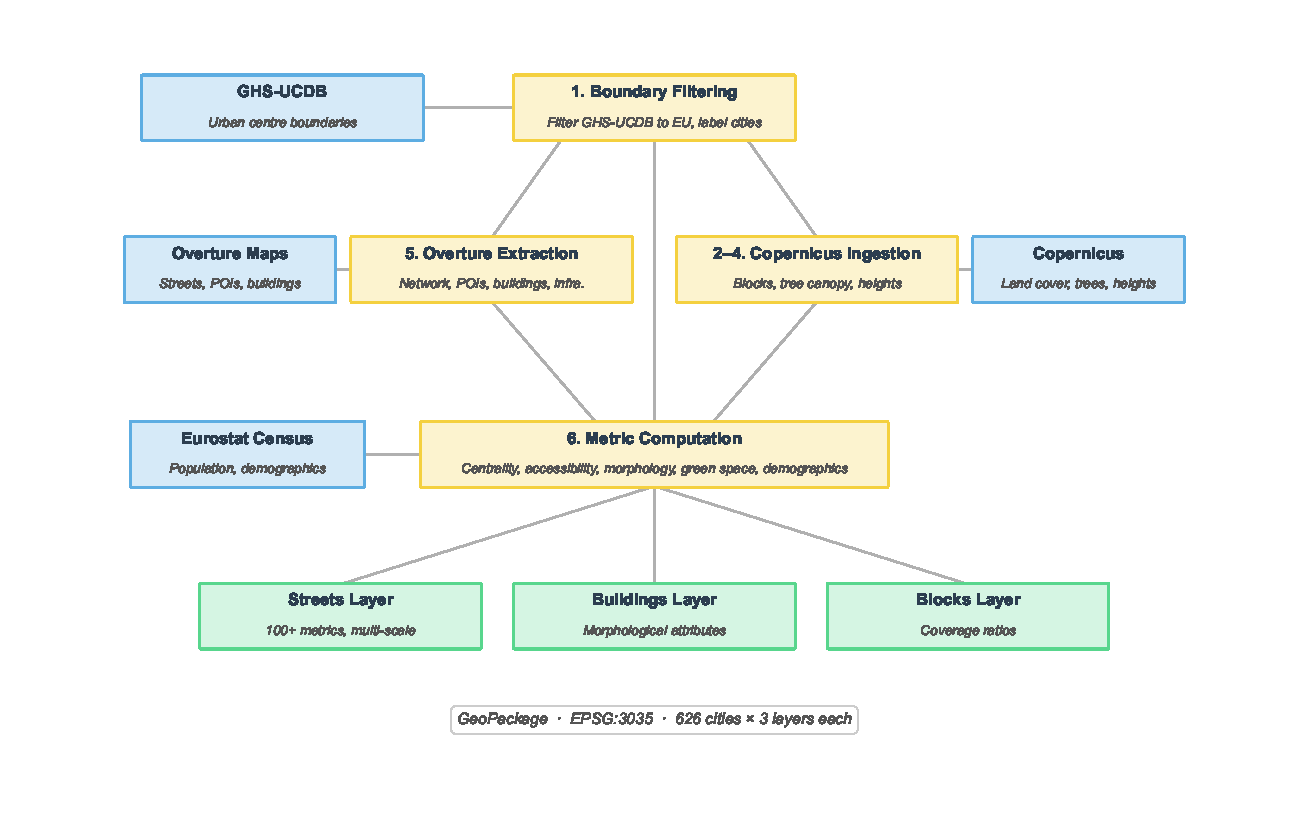
\includegraphics[width=0.85\textwidth]{outputs/figures/fig_pipeline.pdf}
  \caption{\textbf{SOAR-EU processing pipeline.} Four open data sources (blue) feed four processing stages (yellow) that produce three GeoPackage output layers per city (green). Stage~1 filters GHS-UCDB boundaries to the EU and labels cities; Stages~2--5 ingest Copernicus and Overture data in parallel; Stage~6 computes all metrics using the ingested layers, Eurostat census data, and the filtered boundaries.}
  \label{fig:pipeline}
\end{figure}

\subsection{Study Area Definition}
\label{sec:study-area}

Urban boundaries derive from the Global Human Settlement Layer Urban Centre Database (GHS-UCDB) R2024A \cite{ghsl2024}, which defines urban centres using the Degree of Urbanisation (DEGURBA) methodology: contiguous 1$\times$1~km grid cells with $\geq$1,500 inhabitants/km\textsuperscript{2} (or $\geq$50\% built-up surface) and cumulative population $\geq$50,000. Filtering to continental Europe (EPSG:3035) yielded \NCitiesTotal{} urban centres. All meet the $\geq$50,000 population threshold and thus correspond to cities or major urban agglomerations rather than small towns. City names are taken directly from the GHS-UCDB \texttt{GC\_UCN\_MAI\_2025} (Main Urban Centre Name) attribute. Because GHS-UCDB boundaries reflect population density contours rather than administrative units, assigned names may not always correspond to commonly used city names (e.g., a district name rather than the parent municipality).

\subsection{Data Sources}

Table~\ref{tab:sources} summarises input datasets.

Street networks from Overture Maps \cite{overture2026} were cleaned via cityseer \cite{simons2023}, following the automated network-cleaning procedure described in \cite{abdeldayem2026}: disconnected components were removed and degree-2 nodes collapsed. Level-aware processing prevents incorrect merging at bridges or tunnels. The 8\,m cleaning tolerance is deliberately conservative, prioritising consistent processing across all cities over city-specific fine-tuning.

POI categories from Overture's ``places'' theme were mapped to 11 analytical classes (Table~\ref{tab:landuse}; derivation in Section~\ref{sec:landuse-access}), and infrastructure points from Overture's infrastructure theme to three categories (transport, parking, street furniture; Table~\ref{tab:infrastructure}). Land cover and tree canopy derive from Copernicus Urban Atlas \cite{eea2021ua} and Street Tree Layer \cite{eea2021stl} respectively. Building heights were sampled from the Digital Height Model \cite{eea2012bh}.

Demographics from Eurostat Census Grid 2021 \cite{eurostat2024} include population, employment, age structure, nationality, and migration at 1~km\textsuperscript{2} resolution.

\begin{table}[H]
  \centering
  \caption{Input data sources and their roles in the processing pipeline.}
  \label{tab:sources}
  \small
  \begin{tabular}{@{}L{2.5cm}L{1.6cm}L{1cm}L{2.8cm}L{3.2cm}@{}}
    \toprule
    \textbf{Dataset} & \textbf{Source} & \textbf{Year} & \textbf{Licence} & \textbf{Use} \\
    \midrule
    GHS-UCDB R2024A & JRC/GHSL & 2024 & \href{https://commission.europa.eu/legal-notice_en\#copyright-notice}{EC reuse policy} & Urban boundaries \\
    Street networks & Overture Maps & 2026 & \href{https://opendatacommons.org/licenses/odbl/1-0/}{ODbL} & Centrality, accessibility \\
    Points of interest & Overture Maps & 2026 & \href{https://cdla.dev/permissive-2-0/}{CDLA-Permissive-2.0} & Land-use metrics \\
    Building footprints & Overture Maps & 2026 & \href{https://opendatacommons.org/licenses/odbl/1-0/}{ODbL} & Morphology \\
    Urban Atlas & Copernicus & 2021 & \href{https://land.copernicus.eu/en/data-policy}{Copernicus data policy} & Blocks, green space \\
    Street Tree Layer & Copernicus & 2021 & \href{https://land.copernicus.eu/en/data-policy}{Copernicus data policy} & Tree proximity \\
    Height Model & Copernicus & 2012 & \href{https://land.copernicus.eu/en/data-policy}{Copernicus data policy} & Building heights \\
    Census Grid & Eurostat & 2021 & \href{https://commission.europa.eu/legal-notice_en\#copyright-notice}{EC reuse policy} & Demographics \\
    \bottomrule
  \end{tabular}
\end{table}

\subsection{Data Processing Pipeline}

The pipeline comprises six stages executed via Python modules (Table~\ref{tab:pipeline}). All scripts support idempotent execution (existing outputs are skipped unless \texttt{overwrite} is specified), enabling incremental processing and failure recovery.

\begin{table}[H]
  \centering
  \caption{Processing pipeline stages with corresponding Python modules.}
  \label{tab:pipeline}
  \small
  \begin{tabular}{@{}cL{6cm}L{6cm}@{}}
    \toprule
    \textbf{Stage} & \textbf{Module} & \textbf{Description} \\
    \midrule
    1 & \texttt{src.data.generate\_boundary\_polys} & Filter GHS-UCDB boundaries to continental Europe \\
    2 & \texttt{src.data.load\_urban\_atlas\_blocks} & Extract Urban Atlas blocks per boundary \\
    3 & \texttt{src.data.load\_urban\_atlas\_trees} & Extract Street Tree Layer per boundary \\
    4 & \texttt{src.data.load\_bldg\_hts\_raster} & Clip building height rasters per boundary \\
    5 & \texttt{src.data.load\_overture} & Extract Overture data (network, POIs, buildings, infrastructure) \\
    6 & \texttt{src.processing.generate\_metrics} & Compute all metrics per boundary \\
    \bottomrule
  \end{tabular}
\end{table}

For accurate metric computation at boundary edges, input datasets are buffered beyond city boundaries. Street networks are buffered by 10\,km, giving nodes near boundaries a complete network context for centrality calculations. Points of interest, buildings, and infrastructure are buffered by 2\,km, capturing all reachable amenities for boundary-proximate locations. Copernicus land cover and tree canopy data is clipped to boundary bounding boxes for green-space proximity coverage.

\subsection{Metric Computation}
\label{sec:metric-computation}

\subsubsection{Network Centrality}
Network centrality metrics quantify a location's connectivity within the street network and were computed using the cityseer package \cite{simons2023}.

Closeness variants measure how accessible a location is relative to the rest of the network: beta-weighted closeness (gravity index with exponential distance decay), harmonic closeness (sum of inverse distances), Hillier-type closeness (node count divided by average node distance), farness (sum of distances), and street segment density. The density measure (\texttt{cc\_density\_DDD}) is an unweighted count of network nodes, each corresponding to a natural street-segment midpoint after cleaning, reachable within the network-distance threshold; it is not weighted by segment lengths. Betweenness centrality measures how often a location lies on shortest paths between other locations and is computed in both standard and distance-weighted forms.

Metrics were generated using cityseer's shortest-path centrality (\texttt{centrality\_shortest}) at thresholds of 400\,m, 800\,m, 1,200\,m, 1,600\,m, 4,800\,m, and 9,600\,m, corresponding to 5--120 minute walking catchments at 80\,m/min average pedestrian speed. These thresholds span local-to-global catchments: 400\,m captures immediate neighbourhood context; 800\,m reflects typical distances walked to transit; the 1,200--1,600\,m range corresponds to 15-minute walking catchments; 4,800\,m characterises district-scale network structure; and 9,600\,m extends to city-wide connectivity. Centralities are measured using shortest paths (as opposed to angular paths) for greater tolerance of artefacts deriving from automated street cleaning procedures.

\subsubsection{Land-Use and Infrastructure Accessibility}
\label{sec:landuse-access}
Points of interest from Overture Maps were classified into the 11 aggregated land-use categories distributed with the dataset (Table~\ref{tab:landuse}). The aggregation follows Overture's own top-level groupings to the extent possible, rather than imposing a re-engineered taxonomy: most of the 11 categories correspond directly to a single Overture top-level class, with only two consolidations (\texttt{eat\_and\_drink} merging restaurants, bars, and cafés; \texttt{business\_and\_services} merging eleven Overture professional and commercial sub-classes) and two renames (\texttt{public\_services} from \texttt{public\_service\_and\_government}, \texttt{religious} from \texttt{religious\_organization}). The complete mapping from Overture's 2,000+ leaf categories to analytical classes is detailed in Supplementary Material (Section~S2).

Overture's separate infrastructure theme is grouped into three further accessibility categories (transport, parking, and street furniture; Table~\ref{tab:infrastructure}), which receive the identical network-accessibility treatment described below.

Accessibility metrics aggregate POI counts over the street network at the same street-segment locations used for centrality computations, enabling direct comparison between network structure and land-use distribution \cite{simons2023}. Network-based distances are used throughout, rather than Euclidean buffers or zonal aggregation.

For each land-use and infrastructure category, both unweighted counts (reachable POIs within $d_{\max}$) and distance-weighted counts (applying exponential decay $e^{-\beta d}$, where $\beta = 4/d_{\max}$ such that weight falls to approximately 0.018 at the distance threshold) were computed, alongside nearest-distance measures. Distance-weighted counts reflect how amenity usage decays with distance (a caf\'{e} at 100\,m contributes more than one at 1,000\,m), while unweighted counts offer simpler interpretability.

The exponential weight never reaches zero, so an establishment infinitely far would still make an infinitesimal contribution. To keep each measure finite and tied to a walkable catchment, a threshold distance $d_{\max}$ is imposed rather than integrating over the entire network. The decay rate is set at $\beta = 4/d_{\max}$ where the weight has already fallen to under 2\% by the time it reaches $d_{\max}$, thereby discarding the infinitely long tail with minimal impact on the aggregations. The threshold distances are chosen for rounding convenience and the provision of a range of thresholds lets users choose the catchment that suits the intended usage scenario.

Mixed-use diversity was quantified using Hill numbers \cite{hill1973}. Hill numbers at $q=0$ equal richness (count of distinct land-use types); at $q=1$, the exponential of Shannon entropy; at $q=2$, the inverse Simpson index. We compute all three variants in both unweighted and distance-weighted forms, where the distance-weighted forms follow the same weighting conventions as described for land-use accessibility.

\subsubsection{Morphology}
Building and block morphology metrics were computed using the momepy package \cite{fleischmann2019}, which provides standardised urban morphometric functions.

For each building footprint, we compute: area, perimeter, circular compactness, orientation, corners count, shape index, fractal dimension, and shared wall ratio (fraction of perimeter shared with adjacent buildings). Building heights are extracted from the Copernicus Height Model raster by buffering each footprint by 10\,m (one DHM pixel) and averaging valid (non-null) overlapping pixel values. The single-pixel buffer ensures that small footprints (those contained within a single pixel) and footprints with minor misregistration against the 2012 raster still receive a height sample; the trade-off is some smoothing in dense fabric where party-wall neighbours and narrow courtyards fall within the buffer. The height value enables computation of volume and form factor. Floor area (assuming 3\,m floor height) is computed per building as an intermediate for block-level FSI but is not retained as a standalone aggregated metric.

Block morphology uses only built-up Urban Atlas blocks: 14 non-built land-cover classes (green areas, forests, agriculture, water, wetlands, and sports/leisure facilities) are excluded before morphometric computation and aggregation of the metrics to the adjacent streets. For the remaining blocks, we compute geometric properties (area, perimeter, circular compactness, orientation) and Spacematrix indicators \cite{haupt2010}: ground space index (GSI, building footprint area divided by block area), floor space index (FSI, total floor area divided by block area), open space ratio (OSR $= (1 - \text{GSI}) / \text{FSI}$), mean number of storeys (L $= \text{FSI} / \text{GSI}$), and area-weighted mean building height. Blocks exceeding 2\,km\textsuperscript{2} are additionally excluded as oversized infrastructural or transitional polygons (the threshold separates typical urban blocks from large airport, port, industrial, or transitional polygons that occur in the Urban Atlas layer); blocks below 1\% building coverage receive NaN for all Spacematrix metrics, since the ratios become numerically unstable as their denominators (GSI, FSI) approach zero.

Building and block metrics are aggregated to streets via nearest-network-distance assignment within 200\,m and 400\,m thresholds. Each building or block centroid is assigned to the nearest street, and statistics (median and median absolute deviation) are computed across all features within each threshold distance. For building area and volume, sum statistics are additionally retained; for block area, only the sum is additionally retained. Building height is also aggregated (as median and MAD of individual building heights per street).

In addition, a bilateral street-frontage ratio is computed per street segment as a source-robust measure of building continuity. For each street, a 35\,m buffer defines a corridor; all building edges whose midpoint falls inside the corridor and whose nearest street is this one are identified. Per side (left/right of the centreline), only edges within 5\,m of the closest edge are retained, filtering out rear extensions and garages while preserving the primary facade line. The score is the fraction of street length covered by the retained edges on the more-covered side (3\,m trimmed from each end as a junction guard). Unlike shared wall ratio, which requires exact topological contact between adjacent polygon boundaries, frontage ratio depends only on building \emph{presence} along the street edge. It is therefore insensitive to unintended gaps and to the lack of delineation between neighbouring buildings that is characteristic of ML-derived footprints, where segmentation pipelines lack the cadastral subdivision information available to community-contributed sources (see Section~\ref{sec:provenance}).

\subsubsection{Green Space Proximity}
Network distance to nearest green space polygon edge was computed for each street. Green spaces derive from 12 Urban Atlas land cover classes: public and unknown-access urban green areas, forests, herbaceous vegetation, open spaces with little or no vegetation, wetlands, water bodies, pastures, arable land, permanent crops, mixed cultivation, and orchards (full list in Supplementary Material Section~S3). Sports and leisure facility blocks often function as green space (e.g., open playing fields) but can also be heavily built up (e.g., stadiums, indoor arenas); we therefore apply a consistent 20\% building-coverage threshold, including the block as green space when built coverage is below 20\% and excluding it otherwise.

Polygon boundaries are sampled at 20\,m intervals to generate point features for distance calculations, improving accuracy for large or irregularly-shaped polygons. For each street, only the distance to the single nearest sampled point is retained, so a polygon contributes to a given street at most once regardless of how many of its boundary samples lie within range. Tree canopy proximity uses Street Tree Layer polygons with equivalent sampling. Green space and tree canopy areas are also aggregated within walking distances (200\,m, 400\,m, 800\,m) to quantify local coverage.

\subsubsection{Demographic Interpolation}
Census grid values were interpolated to street-segment midpoints using Delaunay-based linear barycentric interpolation (\texttt{scipy.interpolate.griddata}, method \texttt{linear}) from 1\,km grid cell centroids. Interpolated variables include: total population (\texttt{t}), population density (\texttt{density}), male/female counts (\texttt{m}, \texttt{f}), age cohorts (\texttt{y\_lt15}, \texttt{y\_1564}, \texttt{y\_ge65}), employment (\texttt{emp}), nationality (\texttt{nat}, \texttt{eu\_oth}, \texttt{oth}), and migration flows (\texttt{same}, \texttt{chg\_in}, \texttt{chg\_out}). Percentage variants (suffixed with \texttt{\_\%}) are computed for each variable relative to total population. Linear interpolation from 1\,km\textsuperscript{2} source cells produces smooth gradients that do not represent sharp sub-cell discontinuities (industrial estates, large parks, transit corridors); these street-level demographic values should be read as neighbourhood-scale context rather than as fine-grained block-level estimates.

\subsection{Implementation}
\label{sec:implementation}

The pipeline is implemented in Python 3.12 with modules for data ingestion, metric processing, utilities, and land-use classification. Network loading retrieves Overture ``connector'' and ``segment'' themes via STAC, transforms to EPSG:3035, and applies cityseer cleaning (8\,m tolerance, 100-node minimum component size). POI loading maps Overture's 2,000+ raw categories to 23 intermediate classes via a CSV lookup (preserved in the code repository for transparency and reuse), which are then aggregated to the 11 analytical categories distributed with the dataset (Table~\ref{tab:landuse}).

Table~\ref{tab:parameters} summarises the fixed processing parameters ensuring reproducibility across all urban centres.

\begin{table}[!htbp]
  \centering
  \caption{Fixed processing parameters for reproducibility.}
  \label{tab:parameters}
  \small
  \begin{tabular}{@{}L{4cm}L{3cm}L{4.5cm}@{}}
    \toprule
    \textbf{Parameter} & \textbf{Value(s)} & \textbf{Rationale} \\
    \midrule
    Network cleaning tolerance & 8\,m & Consolidate near-parallel edges \\
    Min.\ component size & 100 nodes & Remove disconnected fragments \\
    Centrality thresholds & 400, 800, 1200, 1600, 4800, 9600\,m & 5--120 minute walking catchments \\
    Accessibility thresholds & 200, 400, 800, 1200, 1600\,m & Pedestrian-scale proximity \\
    Morphology aggregation & 200, 400\,m & Immediate building context \\
    Green space proximity & 1600\,m & Extended walkable distance \\
    Green area aggregation & 200, 400, 800\,m & Multi-scale green coverage \\
    \bottomrule
  \end{tabular}
\end{table}

Outputs are written as GeoPackage files in EPSG:3035 following the structure described in Section~\ref{sec:dataset-structure}. Dependencies are pinned via \texttt{pyproject.toml}; core packages include cityseer, momepy, geopandas, and overturemaps.

\subsection{Data Provenance}
\label{sec:provenance}

SOAR-EU integrates data layers with different provenance. Eurostat boundaries, census data, and Copernicus land cover follow documented methodologies with full pan-European coverage. Street networks derive from OpenStreetMap via Overture, whose road coverage is largely complete across urbanised Europe \cite{barringtonleigh2017}.

Building footprints derive from Overture Maps, which conflates multiple sources in a fixed priority order: community-contributed datasets (OpenStreetMap, Esri Community Maps, national cadastres) take precedence over ML-derived datasets (Microsoft ML Building Footprints, Google Open Buildings). When two sources contain the same building (IoU~$\geq$~50\%), the higher-priority source's geometry is retained; ML-derived footprints fill areas not covered by community sources. Each footprint carries a \texttt{sources} attribute recording which dataset contributed it, enabling downstream filtering by provenance.

In European cities, OpenStreetMap is typically the dominant contributor. Herfort et al.\ \cite{herfort2023} analysed OSM building completeness across 13{,}189 urban agglomerations worldwide and found Europe and Central Asia to have the highest regional average (71\%), though within-region coverage remains uneven. Countries with completed cadastral imports---France (DGFiP cadastre), the Netherlands (BAG), and Belgium/Flanders (GRB)---are generally considered to have a high degree of community-sourced building coverage. In contrast, several southern and eastern European countries (including Romania, Bulgaria, Greece, Hungary, and Portugal) lack such imports and, in our data, rely more heavily on Microsoft's ML-derived footprints. Such ML-derived footprints overlap imperfectly with reference building data \cite{minghini2024}, as they are segmented from imagery rather than digitised from cadastre. Across the \NCitiesTotal{} cities in SOAR-EU, the proportion of ML-derived footprints ranges from near-zero in countries with complete cadastral imports to substantial in several southern and eastern European countries; per-city and per-country breakdowns are provided in the accompanying \texttt{building\_source\_counts.csv} and \texttt{building\_source\_by\_country.csv} (summarised in Supplementary~\S\ref{sec:bldg-supp}), and per-city completeness can be cross-referenced against the ohsome OSM-completeness map at \url{https://hex.ohsome.org/#/urban_building_completeness}.

ML-derived footprints expand coverage but introduce quality trade-offs relevant to morphometric computation. Because they are segmented from overhead imagery rather than digitised from cadastral plans, they delineate roof outlines rather than ground-level footprints and can merge adjacent structures into single polygons or leave gaps that break the topological adjacency these metrics rely on. The effect is visible directly in our data: metrics that depend on exact polygon boundary coincidence (particularly shared wall ratio and, to a lesser extent, fractal dimension) are systematically affected, with shared wall ratio showing the strongest negative association between a city's ML fraction and its median value (full coefficients in Supplementary Table~\ref{tab:building_metric_sensitivity}; the within-city test in Supplementary~\S\ref{sec:bldg-supp} confirms this as a per-building artefact rather than a country-level morphological gradient). Metrics based on polygon area and shape (compactness, orientation, shape index) show no significant association with source composition.

POI data derives primarily from commercial and editorial sources (e.g., Meta, Microsoft, Foursquare, OSM) via Overture, with variable coverage relative to official registries; this is characterised in detail in Section~\ref{sec:poi-pattern-characterisation}. Temporal currency and other cross-layer caveats are summarised under Limitations of the Dataset.

\subsection{POI-derived accessibility: source-substitution analysis}
\label{sec:poi-pattern-characterisation}

Because Overture's POI layer aggregates commercial and crowdsourced data of varying completeness, the reliability of derived metrics varies across categories and spatial scales. To characterise where agreement holds and where it does not, we recompute POI-derived outputs against independent official registries in the two countries for which suitable national registries are openly available: France (SIRENE, \NRefCitiesFr{} cities) and the Netherlands (BAG, \NRefCitiesNl{} cities), \NRefCities{} reference cities in total. This validation therefore speaks directly to French and Dutch coverage; cities elsewhere in Europe (particularly in southern and eastern Europe, where OpenStreetMap-derived coverage is less mature) are outside its scope and should be treated with the additional caution discussed under Limitations of the Dataset. We frame the comparison around three questions that capture the main analytical uses of the resulting metrics:
\begin{itemize}
  \item \textbf{How many, relative to elsewhere?} Whether locations are ranked consistently by how much of a particular land use they can access. This is a pattern-agreement question as opposed to one of absolute counts: Overture is known to undercount relative to official registries (further discussed below), so the analytically useful question is whether that undercounting preserves the spatial ordering of accessibility.
  \item \textbf{Where are the hotspots?} Which locations fall in the top tier of activity.
  \item \textbf{How far is the nearest?} Whether the land use is reachable within a given distance threshold.
\end{itemize}
For each question, we measure agreement between Overture- and registry-derived accessibility for every street segment, then summarise within cities and across cities for each category and spatial scale (Figure~\ref{fig:pointa_support_heatmap}; Table~\ref{tab:pointa_minima}).

\subsubsection{Source-substitution replication}

\begin{figure}[!htb]
  \centering
  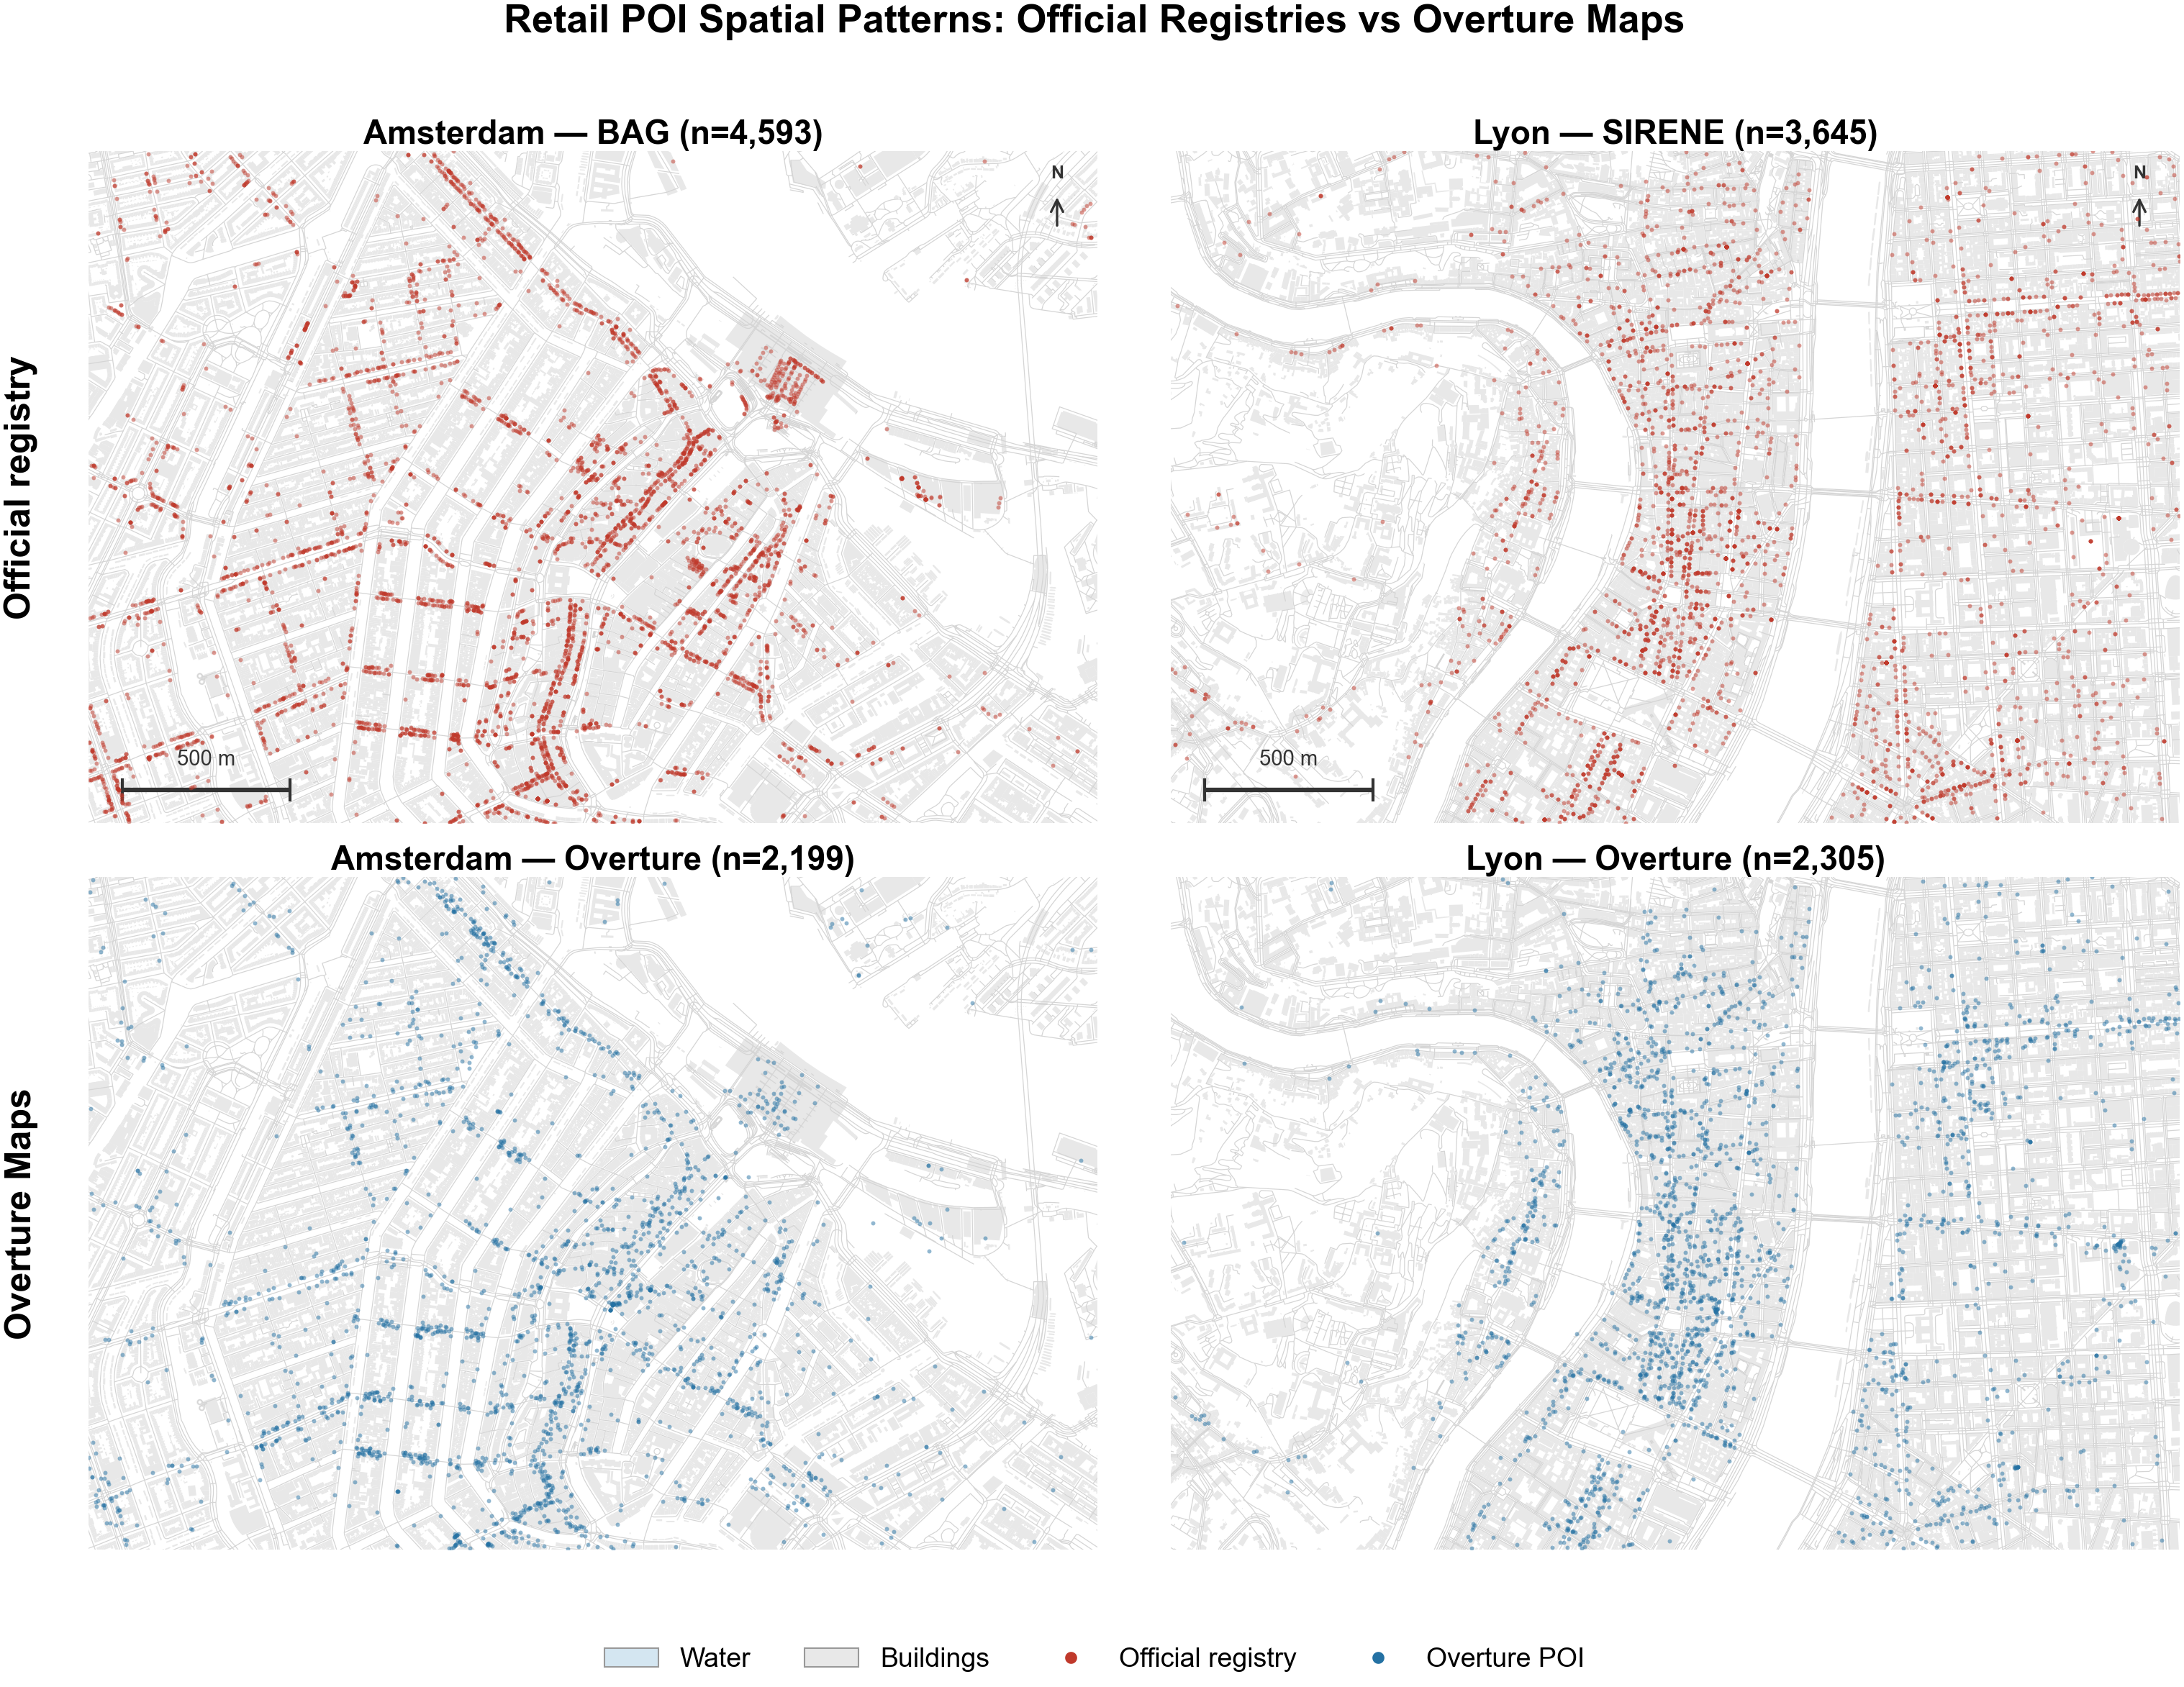
\includegraphics[width=\textwidth]{outputs/figures/fig_poi_spatial_comparison.png}
  \caption{\textbf{Retail POI locations from official registries (top) and Overture Maps (bottom)} for inner-city areas of Amsterdam (BAG; left) and Lyon (SIRENE; right). Point counts differ substantially between sources (Overture undercounts relative to the official registries), but the spatial clustering patterns are broadly consistent.}
  \label{fig:poi_spatial_comparison}
\end{figure}

\begin{figure}[p]
  \centering
  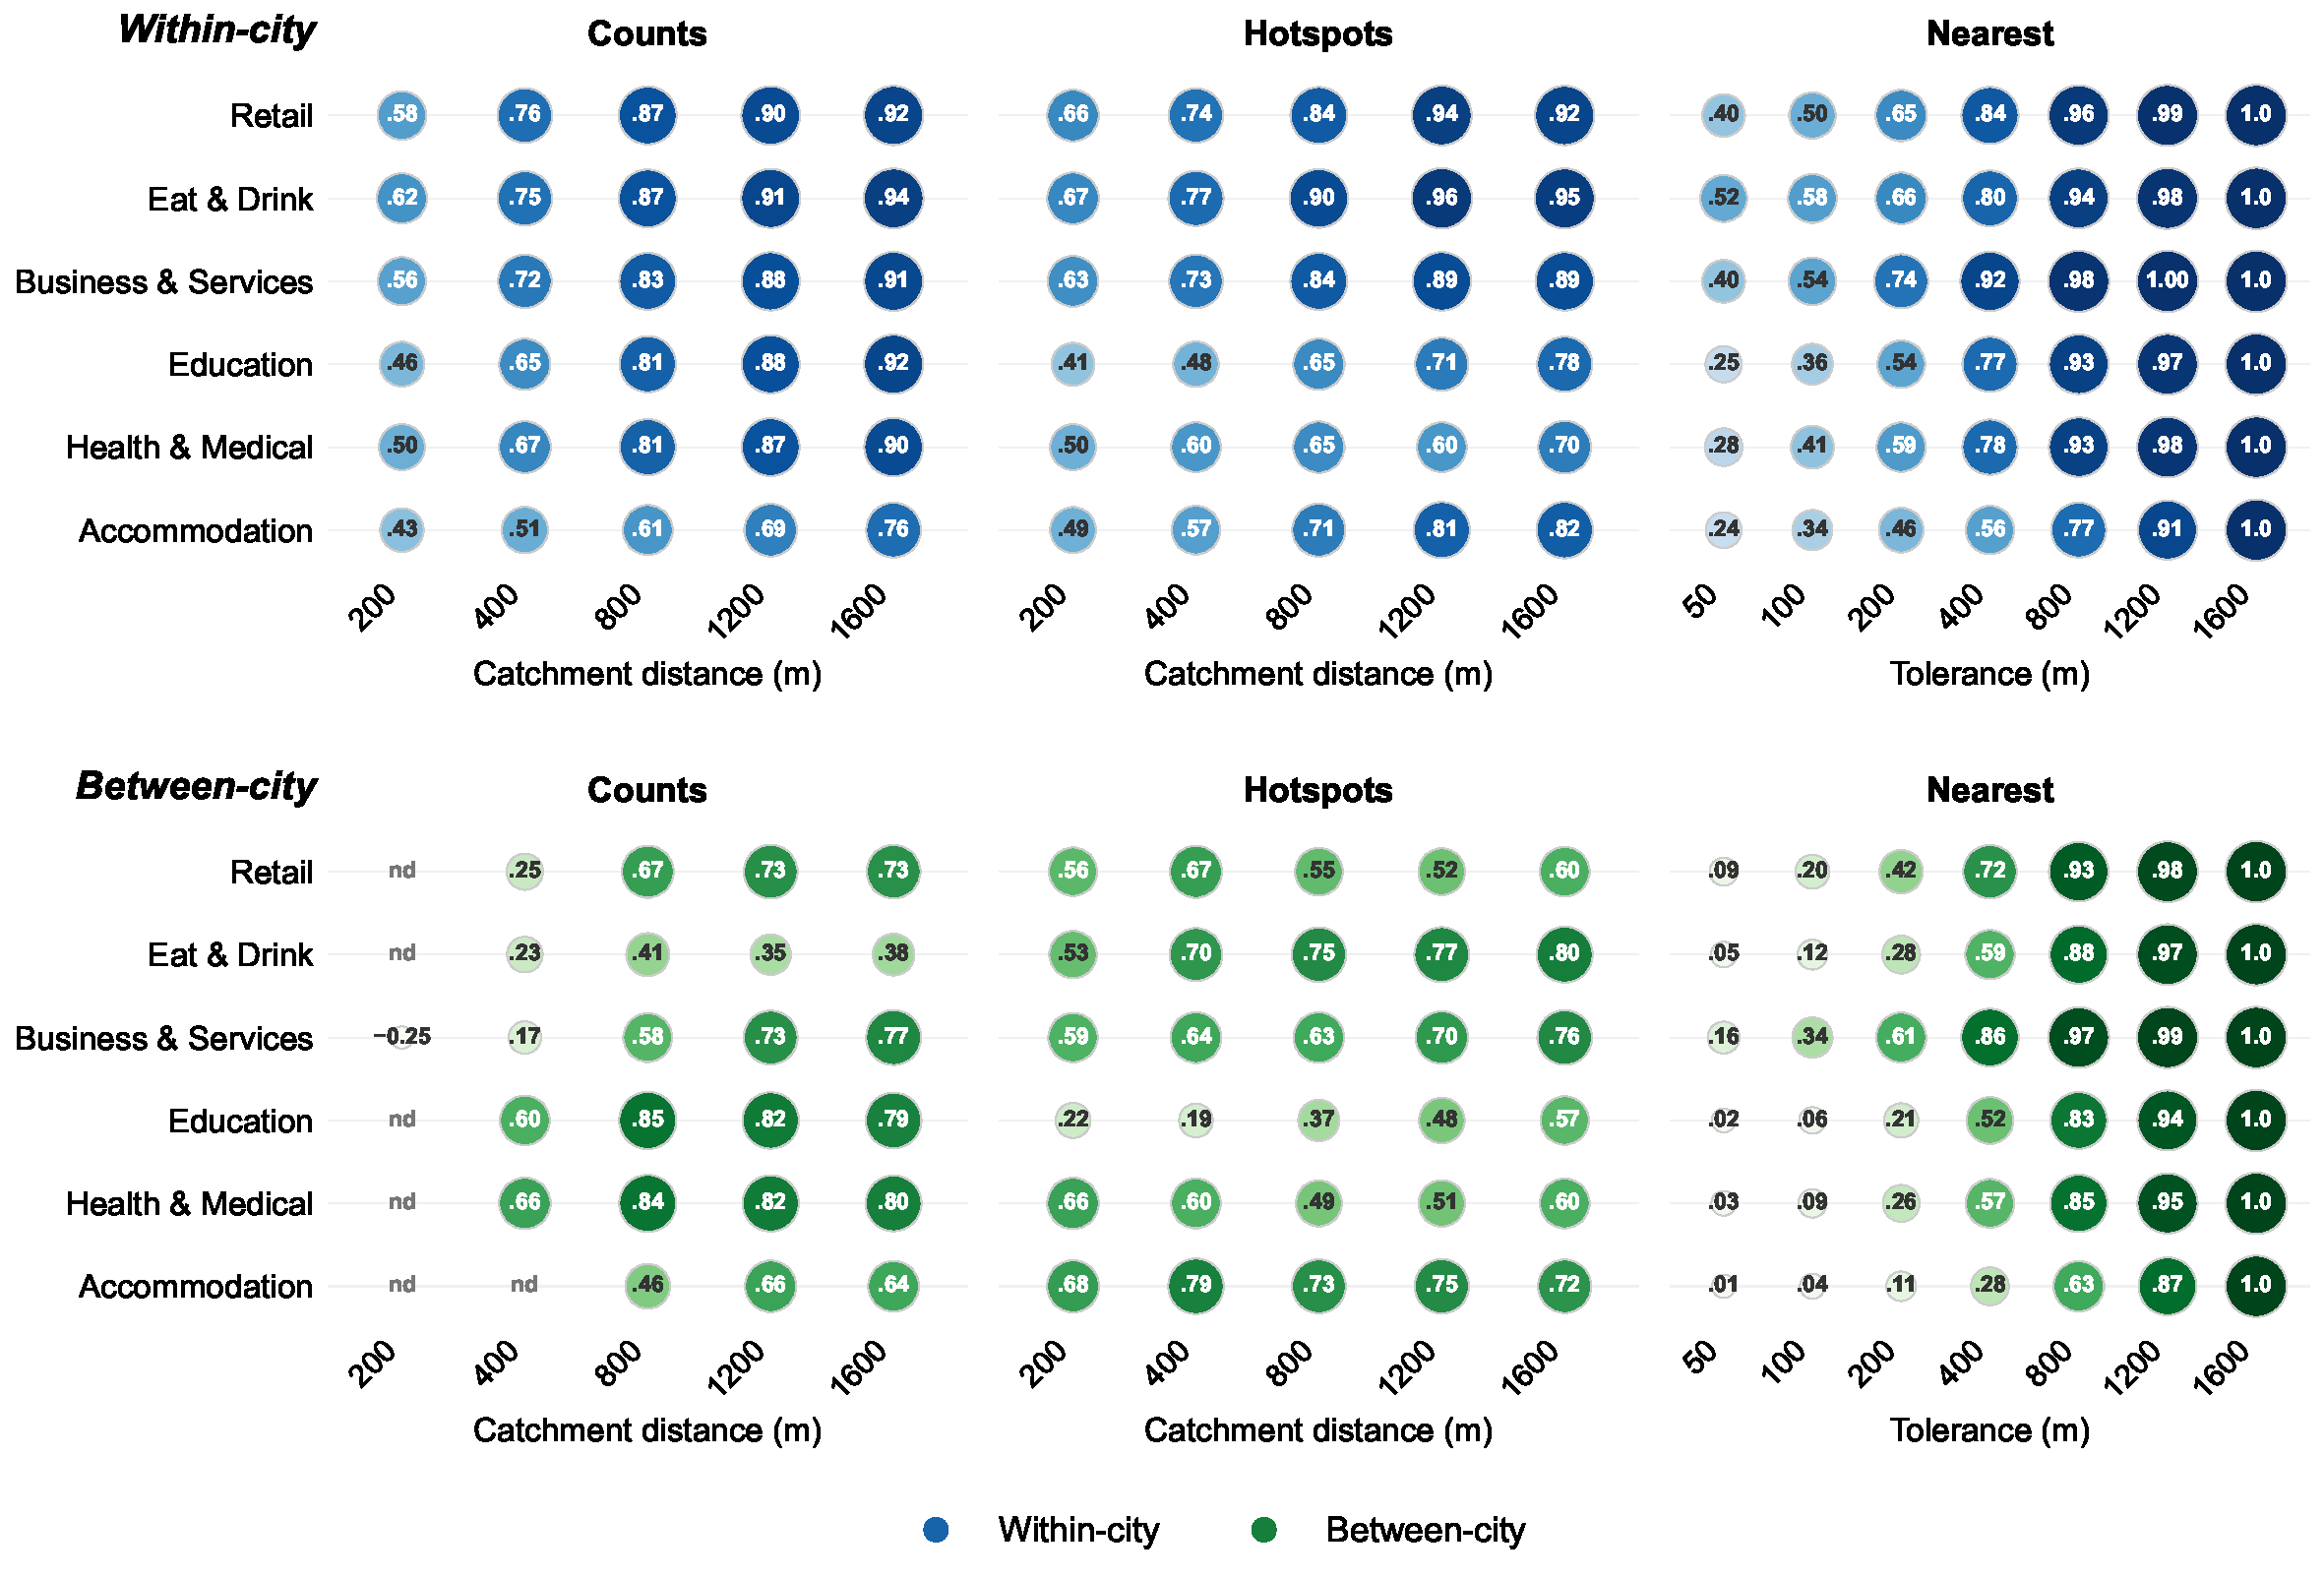
\includegraphics[width=\textwidth]{outputs/figures/fig_pointa_support_heatmap.pdf}
  \caption{\textbf{POI source-substitution agreement.}
    Agreement between Overture- and registry-based accessibility across all category--task--scale combinations. Top row (within-city): Spearman $\rho$ for segment-level rank correlation, top-10\% hotspot overlap, and nearest-distance F1. Bottom row (between-city): Spearman $\rho$ on city-level median counts and hotspot intensity, and harmonic-mean agreement of city-level nearest shares. Bubble size and annotation indicate the median score; colour distinguishes within-city from between-city scope. ``nd'' indicates insufficient data. Full agreement curves with bootstrap CIs appear in Supplementary Figure~\ref{fig:pointa_agreement_panels}.
  }
  \label{fig:pointa_support_heatmap}
\end{figure}

\begin{table}[p]
  \centering
  \caption{Minimum spatial scale (metres) at which each category's median agreement reaches $\geq$70\%, $\geq$75\%, $\geq$80\%, and $\geq$85\% concordance, grouped by scope (within-city, between-city) and metric family. For rank-correlation metrics, concordance is the fraction of observation pairs ranked identically by both sources, computed directly as $(1+\tau)/2$ where $\tau$ is the Kendall rank correlation (thresholds: $\tau \geq 0.40$, $0.50$, $0.60$, $0.70$). For overlap and F1 metrics the concordance fraction is used directly. Dashes indicate no tested scale reached that value.}
  \label{tab:pointa_minima}
  \scriptsize
  \begin{tabular}{@{}lcccccccccccc@{}}
\toprule
\textbf{Category} & \multicolumn{4}{c}{\textbf{Counts}} & \multicolumn{4}{c}{\textbf{Hotspots}} & \multicolumn{4}{c}{\textbf{Nearest}} \\
\cmidrule(lr){2-5}
\cmidrule(lr){6-9}
\cmidrule(lr){10-13}
 & $\geq$70\% & $\geq$75\% & $\geq$80\% & $\geq$85\% & $\geq$70\% & $\geq$75\% & $\geq$80\% & $\geq$85\% & $\geq$70\% & $\geq$75\% & $\geq$80\% & $\geq$85\% \\
\midrule
\textit{Within-city} & \multicolumn{4}{c}{\footnotesize rank concordance} & \multicolumn{4}{c}{\footnotesize top-10\% overlap} & \multicolumn{4}{c}{\footnotesize nearest F1} \\
Retail & 200 & 200 & 400 & 800 & 400 & 800 & 800 & 1200 & 400 & 400 & 400 & 800 \\
Eat \& Drink & 200 & 200 & 400 & 800 & 400 & 400 & 800 & 800 & 400 & 400 & 800 & 800 \\
Business \& Services & 200 & 400 & 800 & 1200 & 400 & 800 & 800 & 1200 & 200 & 400 & 400 & 400 \\
Education & 200 & 400 & 800 & 1200 & 1200 & 1600 & --- & --- & 400 & 400 & 800 & 800 \\
Health \& Medical & 200 & 400 & 800 & 1200 & 1600 & --- & --- & --- & 400 & 400 & 800 & 800 \\
Accommodation & 200 & 800 & 1600 & --- & 800 & 1200 & 1200 & --- & 800 & 800 & 1200 & 1200 \\
\midrule
\textit{Between-city} & \multicolumn{4}{c}{\footnotesize rank concordance (city medians)} & \multicolumn{4}{c}{\footnotesize rank concordance (hotspot intensity)} & \multicolumn{4}{c}{\footnotesize harmonic-mean share} \\
Retail & 800 & 800 & --- & --- & 200 & --- & --- & --- & 400 & 800 & 800 & 800 \\
Eat \& Drink & --- & --- & --- & --- & 200 & 400 & 1600 & --- & 800 & 800 & 800 & 800 \\
Business \& Services & 800 & 1200 & --- & --- & 200 & 1200 & --- & --- & 400 & 400 & 400 & 400 \\
Education & 400 & 400 & 800 & 800 & 1600 & --- & --- & --- & 800 & 800 & 800 & 1200 \\
Health \& Medical & 400 & 400 & 400 & --- & 200 & 200 & --- & --- & 800 & 800 & 800 & 800 \\
Accommodation & 800 & 1200 & --- & --- & 200 & 200 & 200 & --- & 1200 & 1200 & 1200 & 1200 \\
\bottomrule
\end{tabular}

\end{table}

We compute segment-level accessibility metrics twice for each reference city (\NRefCitiesFr{} in France via SIRENE \cite{sirene2026}; \NRefCitiesNl{} in the Netherlands via BAG \cite{bag2026}): once using Overture POIs and once using the official registry as input, holding the street network and all other inputs constant (see Figure~\ref{fig:poi_spatial_comparison} for an example). The question is not whether individual establishments match between sources, but whether the same network-based computations over different POI inputs produce consistent segment-level patterns of accessibility scores. Uncertainty is quantified at two levels: within-city spatial block bootstrap (distance-adaptive blocks, $B = 200$) captures segment-level spatial sampling variability, while a city-level bootstrap ($B = 2{,}000$) treats each city as an independent observation (see Supplementary~\S\ref{sec:poi-supp-bootstrap}). The reference set is concentrated in western Europe and country-specific results are in Supplementary~\S\ref{sec:poi-supp-city-variability}.

The two registries differ in granularity: SIRENE records individual business establishments with fine-grained activity codes that map relatively cleanly onto Overture's commercial categories. BAG records building-level usage \emph{purposes} in coarser classes that require more approximate mapping: a building tagged \texttt{winkelfunctie} (``retail function''), for instance, aggregates a wider activity range than Overture's retail slot. Differences in measured agreement between the two countries may therefore partly reflect harmonisation quality rather than Overture coverage alone, and BAG's coarser categories likely \emph{understate} Dutch agreement relative to a like-for-like comparison. Full harmonisation details, including the snapshot dates and filters used for each registry extract, are in Supplementary~\S\ref{sec:poi-supp-data}.

Six registry-comparable categories are covered: Retail, Eat \& Drink, Accommodation, Health \& Medical, Education, and Business \& Services. No equivalent registry data was available for the remaining categories (e.g., Active Life, Arts \& Entertainment). Formal definitions of all agreement metrics are in Supplementary~\S\ref{sec:poi-supp-metrics}.

\subsubsection{Scale-dependent results}

Agreement varies by category and scale; Figure~\ref{fig:pointa_support_heatmap} summarises all combinations using Spearman $\rho$ for rank-correlation cells, and Table~\ref{tab:pointa_minima} converts these to Kendall $\tau$ concordance for threshold comparison. Agreement curves with bootstrap CIs are in Supplementary Figure~\ref{fig:pointa_agreement_panels}.

We observe that within-city rank agreement increases with scale, while hotspot identification carries greater spatial uncertainty. In the reference cities, rank correlation rises steadily with catchment distance across all categories, with most reaching high concordance by neighbourhood scales (${\sim}$800\,m); Accommodation lags, requiring larger catchments for comparable agreement (Figure~\ref{fig:pointa_support_heatmap}, Table~\ref{tab:pointa_minima}). Hotspot overlap point estimates follow a similar trajectory, but spatial block bootstrap confidence intervals are substantially wider than for rank correlation, reflecting within-city heterogeneity in POI coverage. Nearest-distance F1 rises quickly and shows moderate CI widths. Health \& Medical is the weakest category across all within-city metrics: its sparse and unevenly registered POIs produce both lower point estimates and wider confidence intervals. Accommodation is a secondary outlier.

We find that the data preserves relative distributional patterns across cities, although absolute establishment counts are compressed relative to official registry totals. For between-city comparison across the \NRefCities{} French and Dutch reference cities, we treat each city as a single observation and compare city-level median accessibility scores. Figure~\ref{fig:pointa_support_heatmap} (bottom row) shows strong agreement for Education and Health \& Medical, with weaker but positive ordering for Retail, Eat \& Drink, and Business \& Services. Overture undercounts establishments relative to official registries, particularly for Retail and Eat \& Drink (Supplementary Figure~\ref{fig:pointa_cross_city_scatter}), compressing city-level absolute counts; between-city comparisons therefore reflect broad distributional ordering rather than precise positional ranking.

Among the metric families considered, nearest-distance measures show the strongest and most consistent agreement across both scopes. Within-city nearest-distance F1 rises quickly at moderate tolerances for most categories, and between-city nearest-share agreement is high for most categories by 800\,m (Accommodation requires larger tolerances). Because nearest-distance measures depend only on whether \emph{at least one} POI of the relevant type exists nearby, rather than on exact counts, they are more robust to incomplete coverage and show narrower block bootstrap CIs than hotspot overlap. Nearest-distance metrics therefore reach their agreement thresholds at smaller spatial scales than the count-based or hotspot metrics. These concordance levels are appropriate for analyses that compare distributional patterns across groups (morphological types, city clusters, density bands) rather than precise rankings of individual streets or cities.

%% ============================================================================
%% ETHICS AND DECLARATION
%% ============================================================================
\section*{Declaration of Competing Interest}

The authors declare that they have no known competing financial interests or personal relationships that could have appeared to influence the work reported in this paper.

\section*{Ethics Statement}

This research did not involve human subjects, animal experiments, or data collected from social media platforms. All source datasets are publicly accessible under their respective licenses.

\section*{Limitations of the Dataset}

Although the dataset spans \NCountries{} countries (EU-27 except Cyprus, plus Norway and Switzerland; Liechtenstein has no qualifying urban centre), the quality of contributing data sources, and therefore of derived metrics, is not uniform across this geography. The principal limitations are summarised below.

\begin{itemize}
  \item \emph{Building footprint source composition.} Polygon-precision metrics (shared wall ratio and, to a lesser extent, fractal dimension) are sensitive to whether footprints derive from cadastral or ML-segmented sources (Section~\ref{sec:provenance}). Per-city composition is reported in \texttt{building\_source\_by\_country.csv}, and the bilateral street-frontage ratio (\texttt{frontage\_max}) offers a more source-robust alternative for continuity analyses. Area-based block metrics (GSI, FSI) and shape metrics (compactness, orientation, shape index) show no meaningful association with source composition.

  \item \emph{Geographic scope of POI validation.} The source-substitution validation covers French and Dutch cities only (Section~\ref{sec:poi-pattern-characterisation}), where POI coverage is more mature than in southern and eastern Europe. The scale-dependent agreement curves (Section~S4) therefore characterise the concordance achievable within this benchmark region; cities in Eastern and Southern Europe may show additional category-specific undercounting that these curves do not directly bound.

  \item \emph{Temporal currency.} Source datasets span 2012--2026 (Table~\ref{tab:sources}). The 2012 Copernicus building height raster is the most outdated layer (\BldgHeightsAgeYears{} years old at time of writing), so morphology metrics for cities with substantial post-2012 construction reflect the pre-2012 built form. Because layers differ in vintage, areas of rapid change may show inconsistencies between layers.

  \item \emph{Coverage gaps.} Three metric groups have variable coverage (height-derived attributes, block contextual morphology at 200\,m, and employment demographics), as detailed in Section~\ref{sec:coverage}. Separately, census values are interpolated from 1\,km\textsuperscript{2} grids, which smooths within-cell variation.

  \item \emph{POI accuracy and uncertainty.} As characterised in Section~\ref{sec:poi-pattern-characterisation}, between-city POI-derived comparisons are reliable for broad distributional ordering rather than exact city rankings. Within-city spatial-block bootstrap CIs are substantially wider for hotspot identification (top-10\% overlap) than for rank correlation, particularly for Health \& Medical and Accommodation, where local data sources can help bound the residual uncertainty. Categories without registry comparators (e.g., Active Life, Arts \& Entertainment) lack formal validation.
\end{itemize}

\section*{Declaration of Generative AI and AI-assisted Technologies in the Writing Process}

The original research (pipeline design, data processing, and analysis) was undertaken with minimal AI-assistive technologies. The manuscript itself, together with manuscript-related code and figures, was completed with the aid of Claude (Anthropic). After using this tool, the authors reviewed and edited the content as needed and take full responsibility for the content of the publication.

\section*{CRediT Author Statement}

\noindent\textbf{Gareth Simons}: Conceptualisation, Methodology, Software, Data curation, Writing.\\
\textbf{Kayvan Karimi}: Conceptualisation, Supervision, Review.\\
\textbf{Sepehr Zhand}: Conceptualisation, Review.

\section*{Acknowledgements}

This project has received funding from the European Union's Horizon Europe Research and Innovation Programme under Grant Agreement No.\ \GrantNumber{}, UK Research and Innovation (UKRI) under the UK government's Horizon Europe funding guarantee under grant numbers 10052856 and 10050784.

\section*{Data Availability}

The dataset \cite{soar2026} is available at Zenodo: \ZenodoDoi{} / \ZenodoUrl{}, licensed under the \href{https://opendatacommons.org/licenses/odbl/1-0/}{Open Database License (ODbL 1.0)} to comply with share-alike requirements of the OpenStreetMap-derived content in the Overture Maps layers. The deposit contains the GHS-UCDB-derived \texttt{boundaries.gpkg} file (identifying which urban boundary corresponds to each city), \NCountries{} country-level ZIP archives bundling the \NCitiesTotal{} city GeoPackages with pre-computed metrics (streets, buildings, and blocks layers), and a \texttt{completeness\_coverage.csv} file documenting per-column non-null coverage for every city and layer; it does not redistribute upstream sources, which remain available from their original providers. The independent reference registries used for POI source-substitution testing are publicly available: SIRENE \cite{sirene2026} under Open License 2.0 and BAG \cite{bag2026} under CC Public Domain Mark 1.0.\footnote{Public-domain designations for the BAG vary across Dutch open-data portals (Creative Commons Public Domain Mark 1.0 and CC0 1.0); both dedicate the data to the public domain.}

The processing pipeline is available at \href{https://github.com/UCL/t2e-soar-eu}{github.com/UCL/t2e-soar-eu} (AGPL-3.0, tagged v1.2.0). To reproduce: install dependencies via \texttt{uv sync}, download input datasets per the README, and run the six-stage pipeline (Table~\ref{tab:pipeline}).

\textbf{Supplementary Material} is provided as an appendix: (S1)~complete streets layer schema; (S2)~full land-use classification mapping; (S3)~dataset metadata; (S4)~POI source-substitution methods, agreement curves, and per-city variability.

%% ============================================================================
%% REFERENCES
%% ============================================================================
\begin{thebibliography}{24}

  \bibitem{pesaresi2023} M. Pesaresi, P. Politis, GHS-BUILT-S R2023A -- GHS built-up surface grid [dataset], European Commission, Joint Research Centre, 2023. \url{https://doi.org/10.2905/JRC.939FACR}

  \bibitem{boeing2020} G. Boeing, A multi-scale analysis of 27,000 urban street networks: Every US city, town, urbanized area, and Zillow neighborhood, Environ. Plan. B Urban Anal. City Sci. 47~(4) (2020) 590--608. \url{https://doi.org/10.1177/2399808318784595}

  \bibitem{fleischmann2022} M. Fleischmann, A. Feliciotti, O. Romice, S. Porta, Methodological foundation of a numerical taxonomy of urban form, Environ. Plan. B Urban Anal. City Sci. 49~(4) (2022) 1283--1299. \url{https://doi.org/10.1177/23998083211059835}

  \bibitem{yap2023} W. Yap, F. Biljecki, A global feature-rich network dataset of cities and dashboard for comprehensive urban analyses, Sci. Data 10 (2023) 667. \url{https://doi.org/10.1038/s41597-023-02578-1}

  \bibitem{simons2023} G. Simons, The cityseer Python package for pedestrian-scale network-based urban analysis, Environ. Plan. B Urban Anal. City Sci. 50~(5) (2023) 1328--1344. \url{https://doi.org/10.1177/23998083221133827}

  \bibitem{simons2021thesis} G.D. Simons, Detection and prediction of urban archetypes at the pedestrian scale: computational toolsets, morphological metrics, and machine learning methods, Ph.D. thesis, UCL (University College London), 2021. \url{https://discovery.ucl.ac.uk/id/eprint/10134012/}

  \bibitem{openshaw1984} S. Openshaw, The modifiable areal unit problem, Concepts Tech. Mod. Geogr. 38 (1984). \url{https://www.qmrg.org.uk/catmog/}

  \bibitem{apparicio2008} P. Apparicio, M. Abdelmajid, M. Riva, R. Shearmur, Comparing alternative approaches to measuring the geographical accessibility of urban health services: Distance types and aggregation-error issues, Int. J. Health Geogr. 7 (2008) 7. \url{https://doi.org/10.1186/1476-072X-7-7}

  \bibitem{ghsl2024} European Commission, Joint Research Centre, GHS Urban Centre Database R2024A [dataset], 2024. \url{https://human-settlement.emergency.copernicus.eu/ghs_ucdb_2024.php}

  \bibitem{overture2026} Overture Maps Foundation, Overture Maps Data -- Release 2026-05-20.0 [dataset], 2026. \url{https://docs.overturemaps.org/release/2026-05-20.0/}

  \bibitem{eea2021ua} European Environment Agency, Urban Atlas 2021 [dataset], Copernicus Land Monitoring Service, 2021. \url{https://land.copernicus.eu/en/products/urban-atlas/urban-atlas-2021}. \url{https://doi.org/10.2909/05ae1ee1-e550-4e66-b74d-4926322d981a}

  \bibitem{eea2021stl} European Environment Agency, Street Tree Layer 2021 [dataset], Copernicus Land Monitoring Service, 2021. \url{https://land.copernicus.eu/en/products/urban-atlas/street-tree-layer-stl-2021}

  \bibitem{eea2012bh} European Environment Agency, Building Height 2012 [dataset], Copernicus Land Monitoring Service, 2012. \url{https://land.copernicus.eu/en/products/urban-atlas/building-height-2012}

  \bibitem{eurostat2024} Eurostat, Census 2021 -- Population Grid [dataset], 2024. \url{https://ec.europa.eu/eurostat/web/gisco/geodata/population-distribution/population-grids}

  \bibitem{hill1973} M.O. Hill, Diversity and evenness: a unifying notation and its consequences, Ecology 54~(2) (1973) 427--432. \url{https://doi.org/10.2307/1934352}

  \bibitem{fleischmann2019} M. Fleischmann, momepy: Urban morphology measuring toolkit, J. Open Source Softw. 4~(43) (2019) 1807. \url{https://doi.org/10.21105/joss.01807}

  \bibitem{haupt2010} M. Berghauser Pont, P. Haupt, Spacematrix: Space, Density and Urban Form, NAi Publishers, Rotterdam, 2010.

  \bibitem{herfort2023} B. Herfort, S. Lautenbach, J. Porto de Albuquerque, J. Anderson, A. Zipf, A spatio-temporal analysis investigating completeness and inequalities of global urban building data in OpenStreetMap, Nat. Commun. 14 (2023) 3985. \url{https://doi.org/10.1038/s41467-023-39698-6}

  \bibitem{barringtonleigh2017} C. Barrington-Leigh, A. Millard-Ball, The world's user-generated road map is more than 80\% complete, PLoS ONE 12~(8) (2017) e0180698. \url{https://doi.org/10.1371/journal.pone.0180698}

  \bibitem{minghini2024} M. Minghini, S. Thabit Gonzalez, L. Gabrielli, Pan-European open building footprints: analysis and comparison in selected countries, ISPRS Arch. XLVIII-4/W12-2024 (2024) 97. \url{https://doi.org/10.5194/isprs-archives-XLVIII-4-W12-2024-97-2024}

  \bibitem{sirene2026} INSEE, Base SIRENE des entreprises et de leurs \'{e}tablissements (SIREN, SIRET) [dataset], 2026. \url{https://www.data.gouv.fr/en/datasets/base-sirene-des-entreprises-et-de-leurs-etablissements-siren-siret/}. Open License 2.0 (Etalab).

  \bibitem{bag2026} Kadaster, BAG 2.0 Extract [dataset], 2026. \url{https://www.kadaster.nl/zakelijk/producten/adressen-en-gebouwen/bag-2.0-extract}. CC Public Domain Mark 1.0.

  \bibitem{abdeldayem2026} W.S. Abdeldayem, I. Geddes, A.H. Eldesoky, I. Stavroulaki, G. Simons, M. Berghauser Pont, N. Charalambous, Automated versus hybrid street network modelling for centrality and accessibility analysis, Environ. Plan. B Urban Anal. City Sci. (2026). \url{https://doi.org/10.1177/23998083261433647}

  \bibitem{soar2026} G. Simons, K. Karimi, S. Zhand, SOAR-EU: Scalable Open Automatable Reproducible European Urban Metrics [dataset], Zenodo, 2026. \url{https://doi.org/\ZenodoDoi{}}

\end{thebibliography}

%% ============================================================================
%% SUPPLEMENTARY MATERIAL
%% ============================================================================
\appendix
\renewcommand{\thesection}{S\arabic{section}}

\section{Complete Streets Layer Schema}
\label{sec:streets-schema}

The streets layer contains street segments with computed metrics. Distance thresholds vary by metric type: centrality at 400\,m, 800\,m, 1200\,m, 1600\,m, 4800\,m, 9600\,m; accessibility at 200\,m, 400\,m, 800\,m, 1200\,m, 1600\,m; morphology at 200\,m, 400\,m; green space proximity at 1600\,m; green area aggregation at 200\,m, 400\,m, 800\,m. Table~\ref{tab:complete_streets} provides the complete attribute schema.

\begin{landscape}
  \scriptsize
  \begin{longtable}{@{}L{7cm}L{2cm}L{8cm}L{3cm}@{}}
    \caption{Complete streets layer attribute schema. Suffix \texttt{\_DDD} indicates distance threshold in metres. Source abbreviations: Ovt net = Overture street networks; Ovt POI = Overture POIs; Ovt infra = Overture infrastructure; Ovt bldg = Overture building footprints; UA = Copernicus Urban Atlas; STL = Copernicus Street Tree Layer; CHM = Copernicus Height Model.} \label{tab:complete_streets} \\
    \toprule
    \textbf{Attribute} & \textbf{Type} & \textbf{Description} & \textbf{Source} \\
    \midrule
    \endfirsthead

    \multicolumn{4}{c}%
    {{\tablename\ \thetable{} -- continued from previous page}} \\
    \toprule
    \textbf{Attribute} & \textbf{Type} & \textbf{Description} & \textbf{Source} \\
    \midrule
    \endhead

    \midrule
    \multicolumn{4}{r}{{Continued on next page}} \\
    \endfoot

    \bottomrule
    \endlastfoot

    \multicolumn{4}{l}{\textbf{Geometry and Identifiers}} \\
    \midrule
    \texttt{geometry} & LineString & Street segment geometry (EPSG:3035) & Ovt net \\
    \texttt{ns\_node\_idx} & Integer & Internal network node index & Ovt net \\
    \texttt{x} & Float & Segment midpoint X coordinate (EPSG:3035) & Ovt net \\
    \texttt{y} & Float & Segment midpoint Y coordinate (EPSG:3035) & Ovt net \\
    \midrule

    \multicolumn{4}{l}{\textbf{Network Centrality (Segment-Based, DDD = 400, 800, 1200, 1600, 4800, 9600)}} \\
    \midrule
    \texttt{cc\_beta\_DDD} & Float & Beta-weighted closeness (gravity index with exponential decay) & Ovt net \\
    \texttt{cc\_cycles\_DDD} & Float & Cycle count within threshold & Ovt net \\
    \texttt{cc\_density\_DDD} & Float & Street segment density within threshold & Ovt net \\
    \texttt{cc\_farness\_DDD} & Float & Total network distance to reachable segments & Ovt net \\
    \texttt{cc\_harmonic\_DDD} & Float & Harmonic closeness (sum of inverse distances) & Ovt net \\
    \texttt{cc\_hillier\_DDD} & Float & Hillier-type closeness (node count / avg distance) & Ovt net \\
    \texttt{cc\_betweenness\_DDD} & Float & Segment betweenness centrality & Ovt net \\
    \texttt{cc\_betweenness\_beta\_DDD} & Float & Beta-weighted betweenness centrality & Ovt net \\
    \midrule

    \multicolumn{4}{l}{\textbf{Accessibility -- POI Counts (DDD = 200, 400, 800, 1200, 1600)}} \\
    \midrule
    \texttt{cc\_accommodation\_DDD\_nw} & Integer & Unweighted count of accommodation POIs & Ovt POI \\
    \texttt{cc\_accommodation\_DDD\_wt} & Float & Distance-weighted count of accommodation POIs & Ovt POI \\
    \texttt{cc\_accommodation\_nearest\_max\_1600} & Float & Distance to nearest accommodation POI (m) & Ovt POI \\
    \texttt{cc\_active\_life\_DDD\_nw/wt} & Float & Active life POI counts (unweighted/weighted) & Ovt POI \\
    \texttt{cc\_arts\_and\_entertainment\_DDD\_nw/wt} & Float & Arts and entertainment POI counts & Ovt POI \\
    \texttt{cc\_attractions\_and\_activities\_DDD\_nw/wt} & Float & Attractions and activities POI counts & Ovt POI \\
    \texttt{cc\_business\_and\_services\_DDD\_nw/wt} & Float & Business and services POI counts & Ovt POI \\
    \texttt{cc\_eat\_and\_drink\_DDD\_nw/wt} & Float & Eat and drink POI counts & Ovt POI \\
    \texttt{cc\_education\_DDD\_nw/wt} & Float & Education POI counts & Ovt POI \\
    \texttt{cc\_health\_and\_medical\_DDD\_nw/wt} & Float & Health and medical POI counts & Ovt POI \\
    \texttt{cc\_public\_services\_DDD\_nw/wt} & Float & Public services POI counts & Ovt POI \\
    \texttt{cc\_religious\_DDD\_nw/wt} & Float & Religious POI counts & Ovt POI \\
    \texttt{cc\_retail\_DDD\_nw/wt} & Float & Retail POI counts & Ovt POI \\
    \texttt{cc\_\{category\}\_nearest\_max\_1600} & Float & Distance to nearest POI in category (m) & Ovt POI \\
    \midrule

    \multicolumn{4}{l}{\textbf{Infrastructure Accessibility (DDD = 200, 400, 800, 1200, 1600)}} \\
    \midrule
    \texttt{cc\_transport\_DDD\_nw/wt} & Float & Transport stops/stations counts & Ovt infra \\
    \texttt{cc\_street\_furn\_DDD\_nw/wt} & Float & Street furniture counts (benches, fountains) & Ovt infra \\
    \texttt{cc\_parking\_DDD\_nw/wt} & Float & Parking facility counts & Ovt infra \\
    \midrule

    \multicolumn{4}{l}{\textbf{Mixed-Use Diversity Indices (DDD = 200, 400, 800, 1200, 1600)}} \\
    \midrule
    \texttt{cc\_hill\_q0\_DDD\_nw} & Float & Hill diversity (q=0, richness) unweighted & Ovt POI \\
    \texttt{cc\_hill\_q0\_DDD\_wt} & Float & Hill diversity (q=0, richness) distance-weighted & Ovt POI \\
    \texttt{cc\_hill\_q1\_DDD\_nw} & Float & Hill diversity (q=1, exp Shannon) unweighted & Ovt POI \\
    \texttt{cc\_hill\_q1\_DDD\_wt} & Float & Hill diversity (q=1, exp Shannon) distance-weighted & Ovt POI \\
    \texttt{cc\_hill\_q2\_DDD\_nw} & Float & Hill diversity (q=2, inv Simpson) unweighted & Ovt POI \\
    \texttt{cc\_hill\_q2\_DDD\_wt} & Float & Hill diversity (q=2, inv Simpson) distance-weighted & Ovt POI \\
    \midrule

    \multicolumn{4}{l}{\textbf{Building Morphology (DDD = 200, 400; stat = median, mad; suf = nw, wt)}} \\
    \midrule
    \texttt{cc\_area\_\{stat\}\_DDD\_\{suf\}} & Float & Building area statistics (m\textsuperscript{2}) & Ovt bldg \\
    \texttt{cc\_area\_sum\_DDD\_\{suf\}} & Float & Total building area within threshold (m\textsuperscript{2}) & Ovt bldg \\
    \texttt{cc\_perimeter\_\{stat\}\_DDD\_\{suf\}} & Float & Building perimeter statistics (m) & Ovt bldg \\
    \texttt{cc\_compactness\_\{stat\}\_DDD\_\{suf\}} & Float & Circular compactness ($A / A_{\text{encl}}$) & Ovt bldg \\
    \texttt{cc\_orientation\_\{stat\}\_DDD\_\{suf\}} & Float & Orientation angle (degrees) & Ovt bldg \\
    \texttt{cc\_mean\_height\_\{stat\}\_DDD\_\{suf\}} & Float & Building height (m) & CHM \\
    \texttt{cc\_volume\_\{stat\}\_DDD\_\{suf\}} & Float & Building volume (m\textsuperscript{3}) & Ovt bldg + CHM \\
    \texttt{cc\_volume\_sum\_DDD\_\{suf\}} & Float & Total building volume within threshold (m\textsuperscript{3}) & Ovt bldg + CHM \\
    \texttt{cc\_form\_factor\_\{stat\}\_DDD\_\{suf\}} & Float & Form factor ($S / V^{2/3}$, $S = Ph + A$) & Ovt bldg + CHM \\
    \texttt{cc\_corners\_\{stat\}\_DDD\_\{suf\}} & Float & Corner count & Ovt bldg \\
    \texttt{cc\_shape\_index\_\{stat\}\_DDD\_\{suf\}} & Float & Shape index & Ovt bldg \\
    \texttt{cc\_shared\_wall\_ratio\_\{stat\}\_DDD\_\{suf\}} & Float & Shared wall ratio (fraction of perimeter) & Ovt bldg \\
    \texttt{cc\_fractal\_dimension\_\{stat\}\_DDD\_\{suf\}} & Float & Fractal dimension & Ovt bldg \\
    \texttt{cc\_building\_DDD\_nw/wt} & Float & Building count (unweighted/weighted) & Ovt bldg \\
    \texttt{frontage\_max} & Float & Bilateral street-frontage ratio (0--1); max of left/right building edge coverage within 35\,m corridor & Ovt bldg \\
    \texttt{frontage\_avg} & Float & Mean of left and right frontage coverage & Ovt bldg \\
    \texttt{frontage\_left} & Float & Left-side frontage coverage & Ovt bldg \\
    \texttt{frontage\_right} & Float & Right-side frontage coverage & Ovt bldg \\
    \midrule

    \multicolumn{4}{l}{\textbf{Green Space Proximity (DDD = 200, 400, 800)}} \\
    \midrule
    \texttt{cc\_green\_nearest\_max\_1600} & Float & Distance to nearest green space (m) & UA \\
    \texttt{cc\_trees\_nearest\_max\_1600} & Float & Distance to nearest tree canopy (m) & STL \\
    \texttt{cc\_green\_area\_sum\_DDD\_nw/wt} & Float & Green space area within threshold (km\textsuperscript{2}) & UA \\
    \texttt{cc\_trees\_area\_sum\_DDD\_nw/wt} & Float & Tree canopy area within threshold (km\textsuperscript{2}) & STL \\
    \midrule

    \multicolumn{4}{l}{\textbf{Demographics (interpolated from census grid)}} \\
    \midrule
    \texttt{t} & Float & Total population & Eurostat 2021 \\
    \texttt{density} & Float & Population density (pop / land surface) & Eurostat 2021 \\
    \texttt{m}, \texttt{f} & Float & Male / female population counts & Eurostat 2021 \\
    \texttt{m\_\%}, \texttt{f\_\%} & Float & Male / female percentages & Eurostat 2021 \\
    \texttt{y\_lt15}, \texttt{y\_1564}, \texttt{y\_ge65} & Float & Age cohort counts (under 15, 15--64, 65+) & Eurostat 2021 \\
    \texttt{y\_lt15\_\%}, \texttt{y\_1564\_\%}, \texttt{y\_ge65\_\%} & Float & Age cohort percentages & Eurostat 2021 \\
    \texttt{emp} & Float & Employment count & Eurostat 2021 \\
    \texttt{emp\_\%} & Float & Employment percentage & Eurostat 2021 \\
    \texttt{nat}, \texttt{eu\_oth}, \texttt{oth} & Float & Nationality counts (national, EU other, non-EU) & Eurostat 2021 \\
    \texttt{nat\_\%}, \texttt{eu\_oth\_\%}, \texttt{oth\_\%} & Float & Nationality percentages & Eurostat 2021 \\
    \texttt{same}, \texttt{chg\_in}, \texttt{chg\_out} & Float & Migration counts (same residence, in, out) & Eurostat 2021 \\
    \texttt{same\_\%}, \texttt{chg\_in\_\%}, \texttt{chg\_out\_\%} & Float & Migration percentages & Eurostat 2021 \\
    \midrule

    \multicolumn{4}{l}{\textbf{Block Characteristics (DDD = 200, 400; stat = median, mad; suf = nw, wt)}} \\
    \midrule
    \texttt{cc\_block\_area\_\{stat\}\_DDD\_\{suf\}} & Float & Block area statistics (m\textsuperscript{2}) & UA \\
    \texttt{cc\_block\_perimeter\_\{stat\}\_DDD\_\{suf\}} & Float & Block perimeter statistics (m) & UA \\
    \texttt{cc\_block\_compactness\_\{stat\}\_DDD\_\{suf\}} & Float & Block circular compactness & UA \\
    \texttt{cc\_block\_orientation\_\{stat\}\_DDD\_\{suf\}} & Float & Block orientation (degrees) & UA \\
    \texttt{cc\_block\_covered\_ratio\_\{stat\}\_DDD\_\{suf\}} & Float & Building coverage ratio (GSI) & UA + Ovt bldg \\
    \texttt{cc\_block\_far\_\{stat\}\_DDD\_\{suf\}} & Float & Floor space index (FSI) & UA + Ovt bldg + CHM \\
    \texttt{cc\_block\_osr\_\{stat\}\_DDD\_\{suf\}} & Float & Open space ratio ($= (1 - \text{GSI}) / \text{FSI}$) & UA + Ovt bldg + CHM \\
    \texttt{cc\_block\_l\_\{stat\}\_DDD\_\{suf\}} & Float & Mean storeys ($= \text{FSI} / \text{GSI}$) & UA + Ovt bldg + CHM \\
    \texttt{cc\_block\_mean\_height\_\{stat\}\_DDD\_\{suf\}} & Float & Area-weighted mean building height (m) & UA + Ovt bldg + CHM \\
    \texttt{cc\_block\_DDD\_nw/wt} & Float & Block count (unweighted/weighted) & UA \\

  \end{longtable}
\end{landscape}

\section{Complete Land-Use Classification Schema}
\label{sec:landuse-schema}

Table~\ref{tab:complete_landuse} provides the complete mapping from Overture Maps categories to the 11 analytical land-use classes.

\footnotesize
\begin{longtable}{@{}L{3cm}L{4.5cm}L{5cm}@{}}
  \caption{Complete land-use classification schema mapping Overture categories to analytical classes.} \label{tab:complete_landuse} \\
  \toprule
  \textbf{Analytical Class} & \textbf{Intermediate Class} & \textbf{Overture Categories (examples)} \\
  \midrule
  \endfirsthead

  \multicolumn{3}{c}%
  {{\tablename\ \thetable{} -- continued from previous page}} \\
  \toprule
  \textbf{Analytical Class} & \textbf{Intermediate Class} & \textbf{Overture Categories (examples)} \\
  \midrule
  \endhead

  \midrule
  \multicolumn{3}{r}{{Continued on next page}} \\
  \endfoot

  \bottomrule
  \endlastfoot

  \multirow{3}{*}{eat\_and\_drink} & restaurant & restaurant, bistro, diner \\
  & bar & bar, pub, lounge \\
  & cafe & coffee\_shop, coffee\_roastery \\
  \midrule

  retail & retail & supermarket, grocery\_store, bookstore, florist, pharmacy \\
  \midrule

  \multirow{11}{*}{business\_and\_\allowbreak{}services} & automotive & car\_dealer, car\_wash \\
  & beauty\_and\_spa & hair\_salon, nail\_salon, beauty\_salon \\
  & financial\_service & bank\_credit\_union, insurance\_agency, accountant, tax\_services \\
  & professional\_services & lawyer, cleaning\_services \\
  & real\_estate & real\_estate, real\_estate\_agent \\
  & travel & travel\_agents, visitor\_center \\
  & home\_service & electrician, contractor, roofing \\
  & business\_to\_business & coworking\_space, business \\
  & private\_establishments\_\allowbreak{}and\_corporates & corporate\_office \\
  & mass\_media & print\_media, radio\_station \\
  & pets & veterinarian, pet\_services \\
  \midrule

  public\_services & public\_service\_\allowbreak{}and\_government & town\_hall, courthouse, post\_office, library, community\_center \\
  \midrule

  health\_and\_medical & health\_and\_medical & hospital, doctor, dentist, optometrist \\
  \midrule

  education & education & school, elementary\_school, high\_school, college\_university, driving\_school \\
  \midrule

  accommodation & accommodation & hotel, hostel, motel, guest\_house, bed\_and\_breakfast \\
  \midrule

  active\_life & active\_life & gym, swimming\_pool, playground, bowling\_alley \\
  \midrule

  arts\_and\_\allowbreak{}entertainment & arts\_and\_\allowbreak{}entertainment & cinema, theatre, arcade, auditorium \\
  \midrule

  attractions\_and\_\allowbreak{}activities & attractions\_and\_\allowbreak{}activities & museum, art\_gallery, monument, zoo, aquarium \\
  \midrule

  religious & religious\_organization & church\_cathedral, mosque, synagogue, temple \\
  \midrule

  \multicolumn{3}{l}{\textbf{Infrastructure Categories}} \\
  \midrule

  transport & (aggregated) & bus\_stop, bus\_station, railway\_station, subway\_station, ferry\_terminal, airport, aerialway\_station, helipad \\
  \midrule

  street\_furn & (aggregated) & bench, drinking\_water, fountain, plant, planter, post\_box, picnic\_table \\
  \midrule

  parking & (aggregated) & parking, motorcycle\_parking \\

\end{longtable}
\normalsize

\section{Dataset Metadata}
\label{sec:metadata}

\subsection{GHSL Urban Centre Database (GHS-UCDB) R2024A}

\begin{itemize}
  \item \textbf{Source}: European Commission Joint Research Centre (JRC), Global Human Settlement Layer
  \item \textbf{URL}: \url{https://human-settlement.emergency.copernicus.eu/ghs_ucdb_2024.php}
  \item \textbf{Resolution}: 1km $\times$ 1km grid (DEGURBA methodology)
  \item \textbf{Definition}: Contiguous cells with $\geq$1,500 inhabitants/km$^2$ (or $\geq$50\% built-up surface) and cumulative population $\geq$50,000
  \item \textbf{Reference Year}: 2025 epoch
  \item \textbf{Coverage}: Global (11,422 urban centres; filtered to continental Europe for SOAR-EU)
  \item \textbf{License}: European Commission reuse policy (Decision 2011/833/EU)
  \item \textbf{Processing}: Filtered to continental Europe (EPSG:3035), UK excluded
\end{itemize}

\subsection{Overture Maps Foundation -- Release 2026-05-20.0}

\begin{itemize}
  \item \textbf{Source}: Overture Maps Foundation
  \item \textbf{URL}: \href{https://overturemaps.org/}{overturemaps.org}
  \item \textbf{Release Date}: 2026-05-20
  \item \textbf{Themes Used}:
    \begin{itemize}
      \item Places (POIs): 2,000+ categories
      \item Buildings: Footprints with attributes
      \item Transportation: Road network (connectors and segments)
      \item Infrastructure: Transit stops, street furniture, parking
    \end{itemize}
  \item \textbf{Access Method}: STAC (SpatioTemporal Asset Catalog)
  \item \textbf{License}: ODbL (Transportation, Buildings, Base); CDLA-Permissive-2.0 (Places)
  \item \textbf{Processing}: Clipped to urban boundaries, transformed to EPSG:3035
\end{itemize}

\subsection{Copernicus Urban Atlas 2021}

\begin{itemize}
  \item \textbf{Source}: European Environment Agency / Copernicus Land Monitoring Service
  \item \textbf{URL}: \url{https://land.copernicus.eu/en/products/urban-atlas/urban-atlas-2021}
  \item \textbf{DOI}: \href{https://doi.org/10.2909/05ae1ee1-e550-4e66-b74d-4926322d981a}{10.2909/05ae1ee1-e550-4e66-b74d-4926322d981a}
  \item \textbf{Reference Year}: 2021
  \item \textbf{Resolution}: Minimum Mapping Unit (MMU) 0.25 ha for artificial surfaces
  \item \textbf{Classification}: 28 land cover/use classes (19 urban at 0.25\,ha MMU, 9 rural at 1\,ha MMU)
  \item \textbf{Coverage}: 790 Functional Urban Areas (FUAs) across EU
  \item \textbf{License}: Copernicus data policy (Regulation (EU) No 1159/2013)
  \item \textbf{Processing}: Extracted urban blocks, green spaces; clipped to GHS-UCDB boundaries
  \item \textbf{Green space classes used}: Green urban areas -- public access (14110) and unknown access (14130); Forests (31000), Herbaceous vegetation associations (32000), Open spaces with little or no vegetation (33000), Wetlands (40000), Water (50000), Pastures (23000), Arable land -- annual crops (21000), Permanent crops -- vineyards, fruit trees, olive groves (22000), Complex and mixed cultivation patterns (24000), Orchards at the fringe of urban classes (25000). Sports and leisure facilities (14200) are conditionally included when building coverage is below 20\%
\end{itemize}

\subsection{Copernicus Street Tree Layer 2021}

\begin{itemize}
  \item \textbf{Source}: European Environment Agency / Copernicus Land Monitoring Service
  \item \textbf{URL}: \url{https://land.copernicus.eu/en/products/urban-atlas/street-tree-layer-stl-2021}
  \item \textbf{Reference Year}: 2021
  \item \textbf{Resolution}: 0.5\,m spatial resolution
  \item \textbf{Method}: Very High Resolution imagery interpretation
  \item \textbf{Coverage}: Street trees in Urban Atlas FUAs
  \item \textbf{License}: Copernicus data policy (Regulation (EU) No 1159/2013)
  \item \textbf{Processing}: Clipped to GHS-UCDB boundaries; used for tree proximity calculations
\end{itemize}

\subsection{Copernicus Building Height 2012}

\begin{itemize}
  \item \textbf{Source}: European Environment Agency / Copernicus Land Monitoring Service
  \item \textbf{URL}: \url{https://land.copernicus.eu/en/products/urban-atlas/building-height-2012}
  \item \textbf{Reference Year}: 2012
  \item \textbf{Resolution}: 10\,m $\times$ 10\,m raster
  \item \textbf{Method}: Digital Height Model (DHM) derived from stereo imagery
  \item \textbf{Units}: Metres above ground
  \item \textbf{Coverage}: Urban Atlas FUAs
  \item \textbf{License}: Copernicus data policy (Regulation (EU) No 1159/2013)
  \item \textbf{Processing}: Sampled by buffering each building footprint by 10\,m and averaging valid (non-null) overlapping pixel values; footprints with no valid pixel coverage receive NaN
\end{itemize}

\subsection{Eurostat Census Grid 2021}

\begin{itemize}
  \item \textbf{Source}: Eurostat GEOSTAT project
  \item \textbf{URL}: \url{https://ec.europa.eu/eurostat/web/gisco/geodata/}\\\url{population-distribution/population-grids}
  \item \textbf{Reference Year}: 2021 (Census round)
  \item \textbf{Resolution}: 1km $\times$ 1km grid (INSPIRE compliant)
  \item \textbf{Variables}: Population, employment, demographics, migration
  \item \textbf{Coverage}: EU27 + EFTA
  \item \textbf{License}: European Commission reuse policy (Decision 2011/833/EU); note that Eurostat applies additional dataset-specific download terms for the census population grids (\texttt{TOT\_P\_2006}, \texttt{TOT\_P\_2011}, \texttt{TOT\_P\_2018}, \texttt{TOT\_P\_2021}) on top of the general reuse policy; users redistributing or extending derivative work should consult the GISCO metadata page above for the current population-grid terms.
  \item \textbf{Processing}: Interpolated to street-segment midpoints via grid cell centroids
\end{itemize}

\section{POI Source-Substitution: Methods and Additional Results}
\label{sec:poi-supp}

This supplement provides methodological detail for the POI-source substitution replication described in \S\ref{sec:poi-pattern-characterisation}.

\subsection{Data sources and harmonisation}
\label{sec:poi-supp-data}

The granularity difference between SIRENE and BAG, and its implications for interpreting the cross-country results, is discussed in the main text (\S\ref{sec:poi-pattern-characterisation}). This subsection documents the registry extracts and category mapping used in the replication. Reference set: \NRefCities{} cities (\NRefCitiesFr{} via SIRENE \cite{sirene2026}; \NRefCitiesNl{} via BAG \cite{bag2026}). The codebase records the exact registry extracts used (snapshot dates and filters) alongside the generated outputs.

\subsection{Agreement metrics}
\label{sec:poi-supp-metrics}

Agreement is computed on the SOAR-EU street-segment set for each city, category, and distance threshold. Catchment-based metrics are evaluated at distances of 200, 400, 800, 1200, and 1600\,m; nearest-distance metrics at tolerances of 50, 100, 200, 400, 800, 1200, and 1600\,m. Let $a_u$ and $b_u$ denote the accessibility values (or derived indicators) at segment $u$ under the Overture and registry POI sources, respectively.

\paragraph{Segment-level rank agreement ($\rho$)} For catchment-based accessibility measures (counts and weighted counts), we compute Spearman's rank correlation between $\{a_u\}$ and $\{b_u\}$ across segments. Because Spearman $\rho$ is rank-based and invariant to monotone rescaling, we report values on raw counts.

\paragraph{Hotspot overlap} For each city we identify the top 10\% of segments under each source (by accessibility value; ties broken deterministically) and compute the overlap
\[
  \mathrm{overlap}=\frac{|A\cap B|}{|A|},\quad |A|=|B|=\lceil 0.1\,|U|\rceil
\]
where $U$ is the set of live segments (segments falling within the city boundary, excluding buffer-zone segments used only for computational context) and $A$ and $B$ are the top-decile segment sets under each source. An overlap of 0.6 means roughly 6 in 10 high-accessibility locations are consistently identified across sources.

\paragraph{Nearest-within-tolerance agreement (F1)} For tolerance $t$ (50--1600\,m), define the binary indicator $p_u(t)=\mathbb{1}[\mathrm{nearest}_a(u)\leq t]$ and $q_u(t)=\mathbb{1}[\mathrm{nearest}_b(u)\leq t]$. We report the F1 score (harmonic mean of precision and recall) between $\{p_u(t)\}$ and $\{q_u(t)\}$ across segments, alongside precision/recall diagnostics.

\paragraph{Between-city ordering} For catchment-based metrics, we test whether city-level summaries are consistent across sources. Each city's accessibility distribution is summarised by its median count (for count comparisons) and the median of its top-decile counts (for hotspot intensity comparisons). We report Spearman $\rho$ computed across the \NRefCities{} cities, treating each city's summary statistic as a single observation. Bootstrap confidence intervals are obtained by resampling cities with replacement ($B=2{,}000$).

\paragraph{City-level nearest share agreement (harmonic mean)} For each city, the ``share within tolerance'' is the proportion of segments with $\mathrm{nearest} \leq t$. We summarise agreement in these shares using their harmonic mean
\[
  H(p,q)=\frac{2pq}{p+q},
\]
where $p$ and $q$ are the per-city shares under each source. This symmetric agreement score on prevalence levels, which we term the \emph{share harmonic mean}, is analogous to the S{\o}rensen--Dice coefficient. We report the median across cities.

\subsection{Bootstrap uncertainty}
\label{sec:poi-supp-bootstrap}

Uncertainty is estimated at two levels.

\emph{Within-city}: per-city agreement statistics (Spearman $\rho$, hotspot overlap, nearest F1) are accompanied by spatial block bootstrap confidence intervals. Segments are assigned to square grid cells whose side length equals the catchment distance being tested (e.g.\ 200\,m blocks for the 200\,m metric, 1{,}600\,m blocks for the 1{,}600\,m metric), blocks are resampled with replacement ($B=200$), and the statistic is recomputed on each resample. This distance-adaptive blocking matches the spatial autocorrelation range at each scale, avoiding both under-estimation of uncertainty (blocks too small relative to the catchment, failing to account for the spatial dependence the metric induces) and unnecessary loss of power (blocks too large, discarding within-block information). For the summary plots and heatmap, we report the median score across cities alongside the median of the per-city block-bootstrap CI bounds, so that the displayed confidence band reflects typical within-city spatial uncertainty rather than a single city's interval.

\emph{Between-city}: the city-level bootstrap ($B=2{,}000$ resamples with replacement) treats each city as an independent observation, quantifying the sensitivity of the cross-city median to the composition of the reference set.

These intervals quantify sampling variability within the French--Dutch reference set; they do not bound potential differences in Overture coverage patterns for cities outside this reference region.

\subsection{Reference thresholds}
\label{sec:poi-supp-decision}

Agreement scores are reported continuously with bootstrap CIs. For convenience, Table~\ref{tab:pointa_minima} shows the minimum spatial scale at which the median score first reaches four concordance thresholds ($\geq$70\%, $\geq$75\%, $\geq$80\%, $\geq$85\%). Concordance expresses the fraction of pairwise comparisons on which both sources agree: for rank-correlation metrics it equals $(1+\tau)/2$ where $\tau$ is the Kendall rank correlation, computed directly from the data (corresponding $\tau$ thresholds: $\geq$0.40, 0.50, 0.60, 0.70). This gives the proportion of observation pairs (nodes within a city, or cities in the cross-city comparison) ranked in the same order by both Overture and the official registry. For hotspot overlap and F1 metrics, the score is already a proportion and the concordance fraction is used directly as the threshold.

\subsection{Agreement curves}
\label{sec:poi-supp-agreement-curves}

\begin{figure}[!htb]
  \centering
  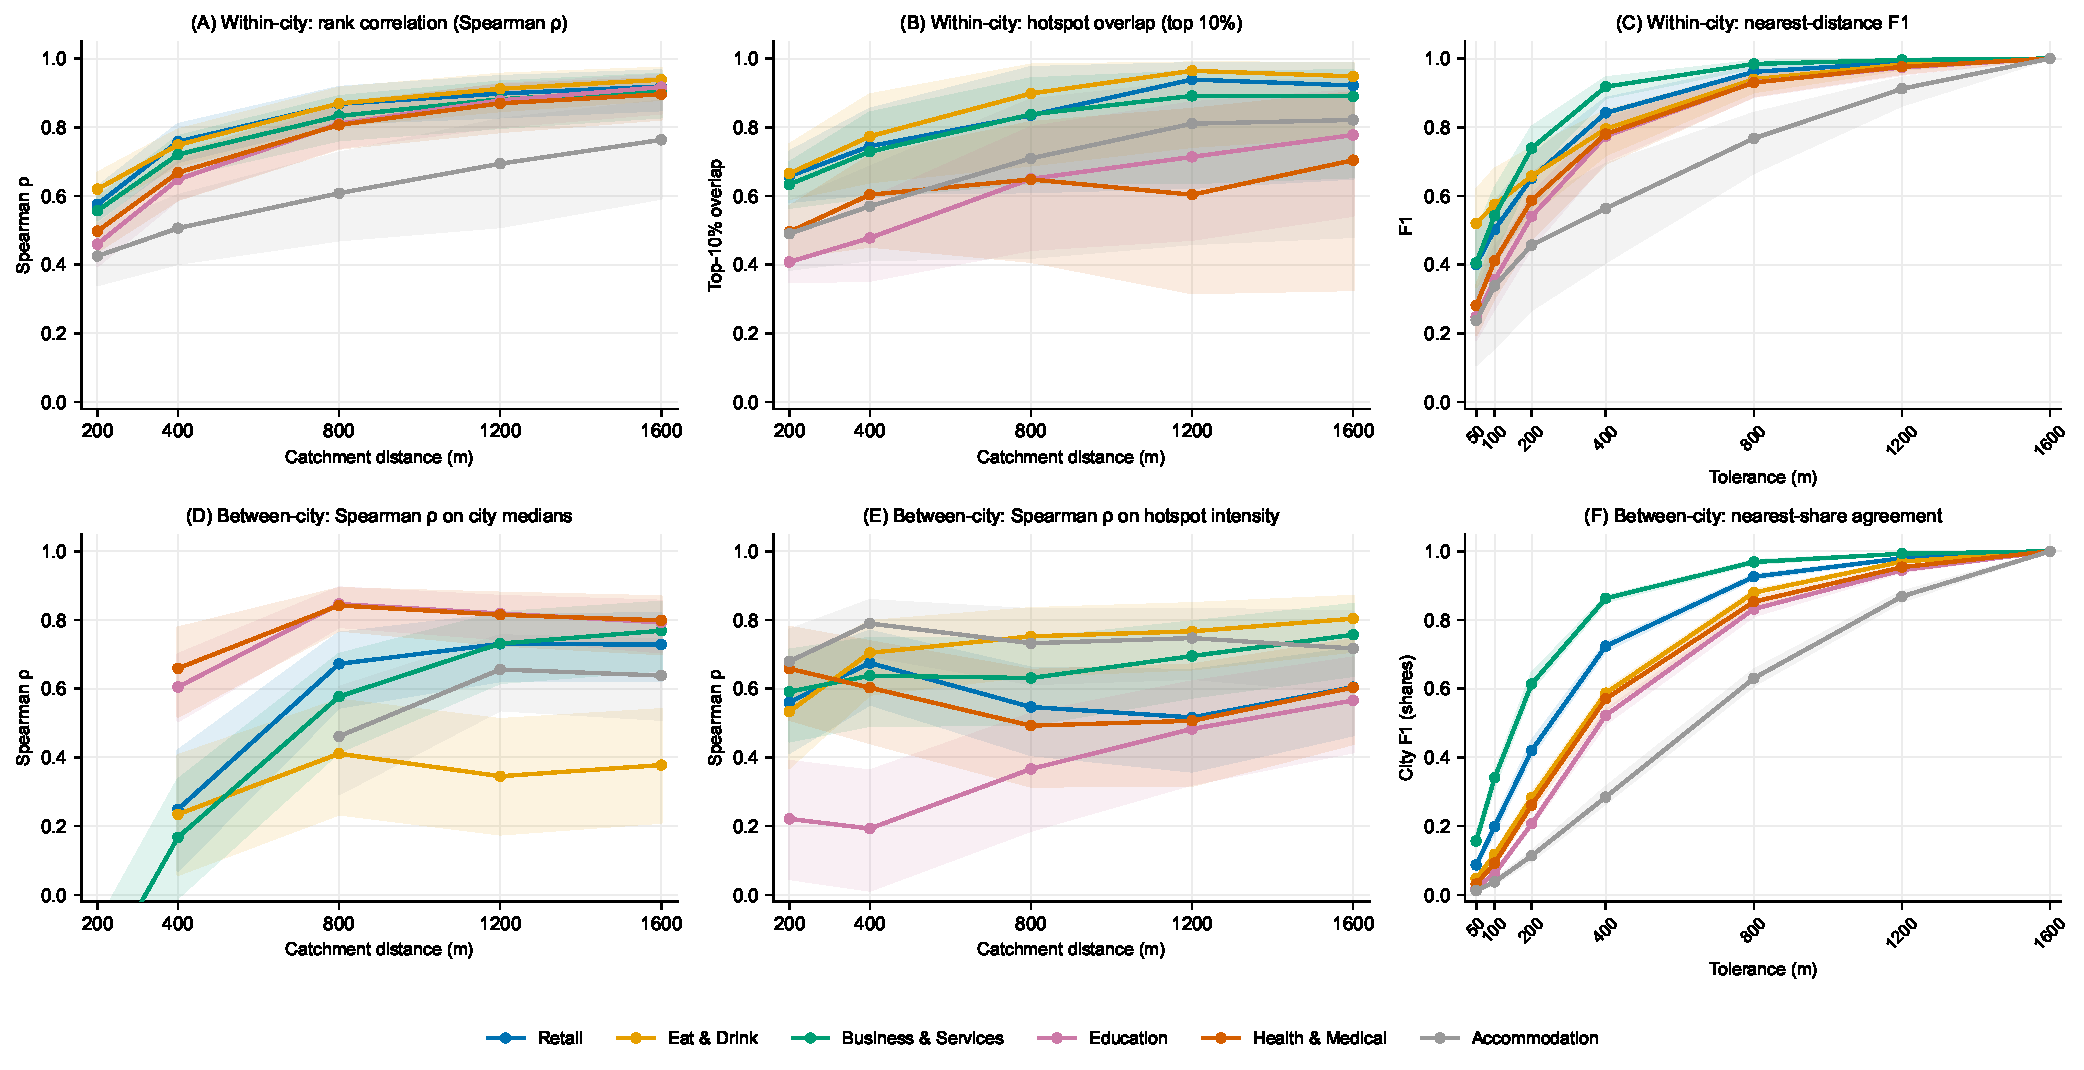
\includegraphics[width=\textwidth]{outputs/figures/fig_pointa_agreement_panels.pdf}
  \caption{\textbf{POI source-substitution agreement by category, task, and spatial scale.}
    \NRefCities{} reference cities. Top row (within-city): (A)~rank correlation (Spearman $\rho$), (B)~hotspot overlap, and (C)~nearest-within-tolerance F1; shaded bands show 95\% spatial block bootstrap CIs (distance-adaptive blocks, $B=200$). Bottom row (between-city): (D)~Spearman $\rho$ on city-level median counts, (E)~Spearman $\rho$ on city-level hotspot intensity, and (F)~harmonic-mean agreement of city-level nearest shares; shaded bands show 95\% city-level bootstrap CIs ($B=2{,}000$).
  }
  \label{fig:pointa_agreement_panels}
\end{figure}

\subsection{Per-city variability}
\label{sec:poi-supp-city-variability}

The main-text figures report median agreement across reference cities. Figure~\ref{fig:pointa_city_variability} shows the underlying per-city distributions at two representative catchment distances (400\,m and 800\,m). The strip plots confirm that the medians are not driven by a small number of outlier cities: at 800\,m most categories have tight distributions for rank correlation, with the bulk of cities exceeding 80\% concordance. Accommodation and Health \& Medical remain consistently the weakest categories with the widest spreads. Figure~\ref{fig:pointa_cross_city_scatter} complements this by plotting city-level median accessibility (log-transformed counts) from Overture against registry values at 800\,m; points falling below the identity line indicate systematic undercounting by Overture, particularly for Retail and Eat \& Drink.

\begin{figure}[p]
  \centering
  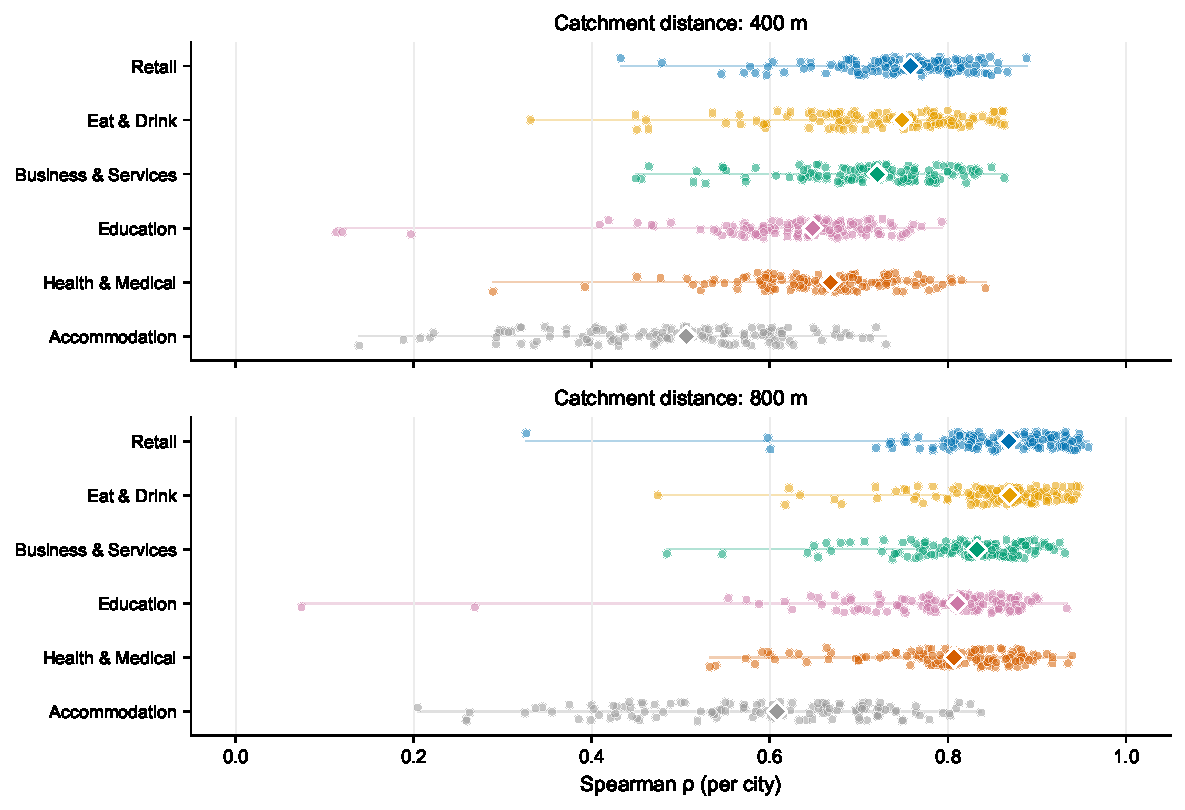
\includegraphics[width=0.88\textwidth]{outputs/figures/fig_pointa_city_variability.pdf}
  \caption{\textbf{Per-city rank correlation spread.}
    Distribution of Spearman $\rho$ (segment-level unweighted counts) across \NRefCities{} reference cities at 400\,m and 800\,m catchments. Points show individual cities; diamonds mark medians.
  }
  \label{fig:pointa_city_variability}

  \vspace{0.5em}

  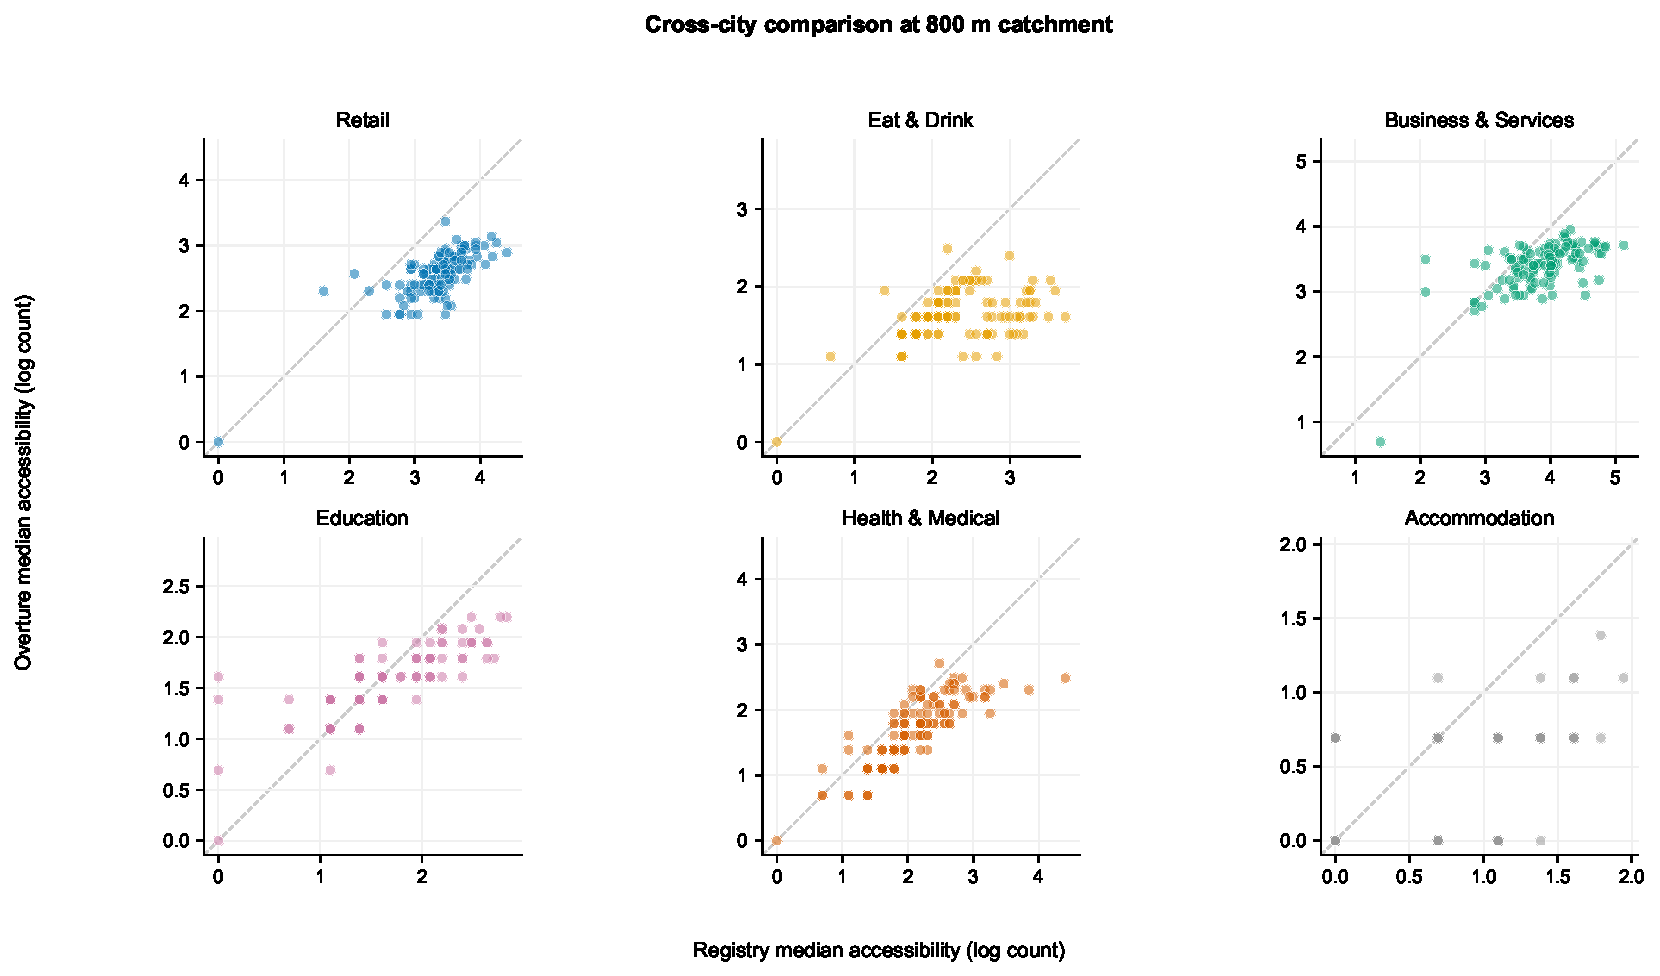
\includegraphics[width=0.88\textwidth]{outputs/figures/fig_pointa_cross_city_scatter.pdf}
  \captionof{figure}{\textbf{Cross-city comparison at 800\,m catchment.}
    Each point is one reference city. Axes show median log-transformed POI counts from registry and Overture sources; the dashed line marks identity. The predominance of points below the line indicates systematic undercounting by Overture, especially for Retail and Eat \& Drink.
  }
  \label{fig:pointa_cross_city_scatter}
\end{figure}

\subsection{Distance-weighted accessibility}
\label{sec:poi-supp-weighted}

The main-text results use unweighted POI counts (the number of establishments reachable within each catchment distance). An alternative is distance-weighted counts, where each POI's contribution decays with network distance, giving greater weight to nearer establishments.

At the same catchment distance, weighted counts produce lower concordance than unweighted counts (typically 3--5 percentage points for rank correlation, 5--8 for hotspot overlap), because the gravity weighting amplifies the effect of small geocoding offsets between sources. However, the weighted measure at 800\,m still exceeds the unweighted measure at 400\,m across all categories, since the larger catchment more than compensates for the concordance lost to weighting. This is relevant for applications that prefer distance-weighted accessibility: reliable concordance is achievable at 800\,m or above. The nearest-distance columns are unchanged, as they do not involve count aggregation.

\clearpage
\section{Building Footprint Source Composition and Metric Sensitivity}
\label{sec:bldg-supp}

This supplement documents the provenance composition of the Overture Maps building footprints used in SOAR-EU and quantifies its effect on derived morphometric indicators.

\subsection{Source classification}
\label{sec:bldg-supp-classification}

Each Overture building footprint carries a \texttt{sources} JSON array whose first element identifies the contributing dataset. We classify these into two groups: \emph{community-contributed} (OpenStreetMap, Esri Community Maps, national cadastral agencies) and \emph{ML-derived} (Microsoft ML Buildings, Google Open Buildings). Community-contributed footprints are digitised or imported from authoritative cadastral sources and generally preserve individual building boundaries; ML-derived footprints are segmented from satellite imagery and may merge adjacent buildings into single polygons or introduce unintended gaps between genuinely attached structures.

Across the \NCitiesTotal{} cities, the footprints draw on several source datasets: OpenStreetMap (dominant in most European cities), Esri Community Maps, Microsoft ML Buildings, and, in Spain, the Instituto Geogr\'{a}fico Nacional cadastre. Country-level aggregates reveal a clear geographic gradient (Table~\ref{tab:building_source_country}; Figure~\ref{fig:building_source_map}): the Netherlands, France, Switzerland, and Belgium are dominated by community sources, while Romania, Spain, Greece, and Bulgaria rely substantially on ML-derived footprints. The per-city ML fraction (Min and Max columns of Table~\ref{tab:building_source_country}) spans from zero in several cadastral-import cities to a large majority in the most ML-reliant. Per-city counts by dataset and country-level summaries are provided in the accompanying CSV files.

\begin{table}[!htb]
  \centering
  \caption{Building footprint source composition by country, sorted by ML-derived fraction (ascending). ML~(\%) is the proportion of footprints from ML-derived sources (primarily Microsoft ML Buildings); Min and Max show the per-city range within each country.}
  \label{tab:building_source_country}
  \scriptsize
  \begin{tabular}{@{}lrrrrr@{}}
  \toprule
  \textbf{Country} & \textbf{Cities} & \textbf{Buildings} & \textbf{ML (\%)} & \textbf{Min (\%)} & \textbf{Max (\%)} \\
  \midrule
  Netherlands & 43 & 6,209,242 & 1.6 & 0.0 & 20.6 \\
  Switzerland & 17 & 794,674 & 4.1 & 0.0 & 11.6 \\
  Luxembourg & 1 & 40,614 & 4.4 & 4.4 & 4.4 \\
  France & 73 & 10,245,743 & 4.5 & 0.0 & 15.2 \\
  Belgium & 16 & 2,627,084 & 5.2 & 1.0 & 16.2 \\
  Ireland & 5 & 769,998 & 5.4 & 3.3 & 8.4 \\
  Norway & 7 & 606,824 & 6.6 & 4.8 & 10.1 \\
  Finland & 6 & 367,553 & 7.8 & 6.2 & 13.5 \\
  Austria & 8 & 688,439 & 8.1 & 4.6 & 18.4 \\
  Denmark & 5 & 647,562 & 8.4 & 5.7 & 9.4 \\
  Estonia & 2 & 102,363 & 8.5 & 6.1 & 13.5 \\
  Germany & 99 & 11,601,375 & 8.8 & 0.1 & 35.7 \\
  Slovakia & 7 & 303,986 & 13.9 & 10.6 & 19.4 \\
  Slovenia & 2 & 98,624 & 15.3 & 13.4 & 19.0 \\
  Lithuania & 4 & 228,098 & 15.7 & 7.8 & 27.1 \\
  Latvia & 2 & 180,865 & 16.1 & 15.8 & 16.7 \\
  Czechia & 12 & 763,959 & 16.7 & 11.6 & 22.1 \\
  Italy & 88 & 4,246,128 & 17.4 & 3.0 & 81.0 \\
  Sweden & 17 & 793,793 & 18.5 & 0.7 & 50.7 \\
  Poland & 63 & 3,612,250 & 18.6 & 4.8 & 37.1 \\
  Croatia & 5 & 272,798 & 24.6 & 16.6 & 33.8 \\
  Hungary & 13 & 944,965 & 27.3 & 16.8 & 61.3 \\
  Portugal & 8 & 916,488 & 27.6 & 18.5 & 57.3 \\
  Bulgaria & 6 & 290,571 & 30.8 & 23.8 & 46.9 \\
  Greece & 8 & 871,146 & 31.3 & 7.5 & 94.9 \\
  Spain & 79 & 3,363,448 & 46.3 & 4.7 & 94.9 \\
  Romania & 29 & 1,319,339 & 48.0 & 23.6 & 86.1 \\
  Malta & 1 & 49,893 & 54.8 & 54.8 & 54.8 \\
  \bottomrule
\end{tabular}
\end{table}

\begin{figure}[!htb]
  \centering
  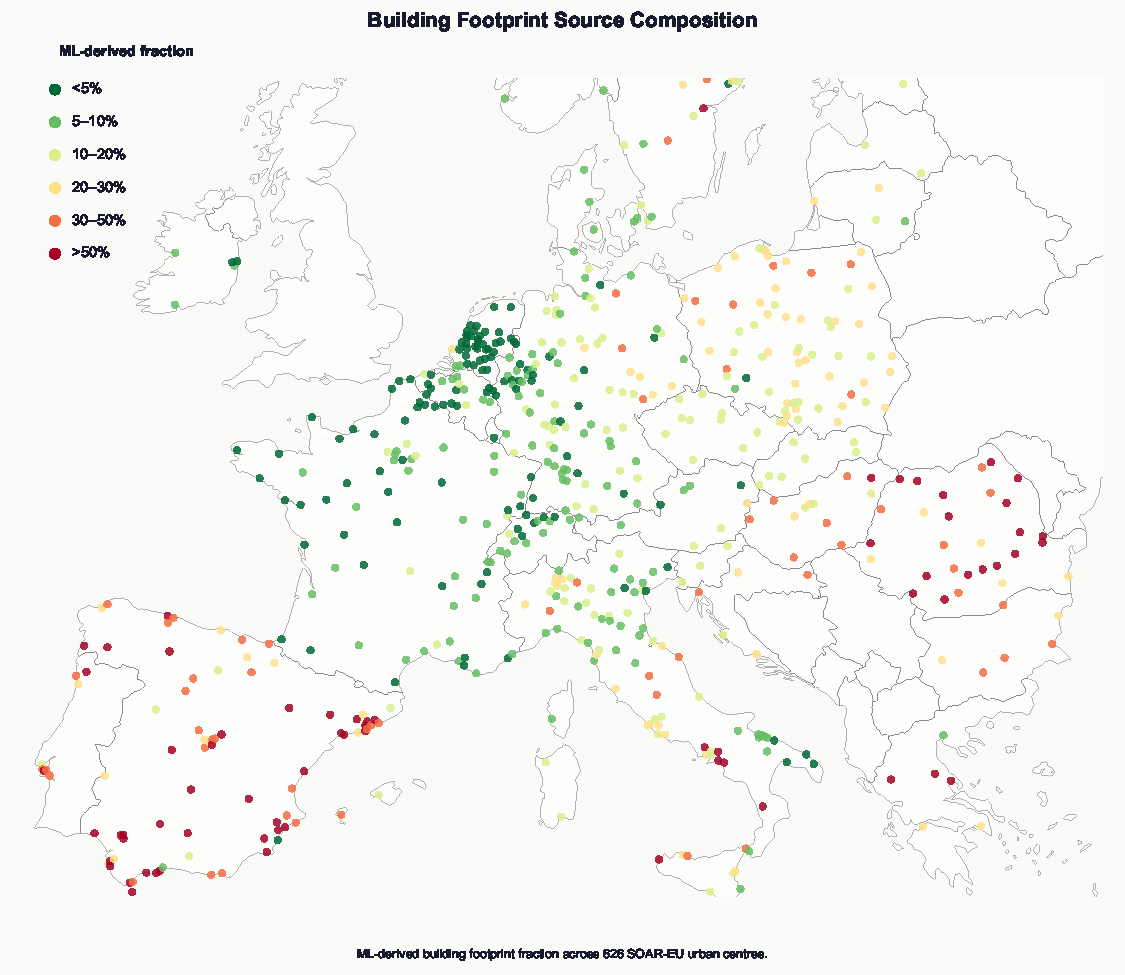
\includegraphics[width=\textwidth]{outputs/figures/fig_building_source_map.pdf}
  \caption{ML-derived building footprint fraction across the \NCitiesTotal{} SOAR-EU urban centres. Cities in western and northern Europe (France, Netherlands, Belgium, Germany) are dominated by community-contributed sources; cities in southern and eastern Europe (Romania, Spain, Greece, Bulgaria) rely more heavily on ML-derived footprints.}
  \label{fig:building_source_map}
\end{figure}

\subsection{Effect on morphometric indicators}
\label{sec:bldg-supp-sensitivity}

We test for source-driven bias at two levels.

\paragraph{Cross-city correlations.} For each morphometric indicator, we compute the Spearman correlation between each city's ML fraction and its median metric value across the \NCitiesTotal{} cities (Table~\ref{tab:building_metric_sensitivity}). Shared wall ratio shows the strongest negative association: cities with more ML-derived buildings have lower shared wall ratios. This cross-city correlation conflates two effects: a genuine morphological gradient (countries with higher ML fractions---Romania, Bulgaria, Greece---also have more freestanding housing stock) and a data artefact (ML-derived footprints underestimate shared walls due to polygon boundary gaps). The within-city test below isolates the artefact component. Perimeter, area, and volume are also positively associated, partly reflecting the tendency of ML segmentation to merge adjacent buildings into larger polygons and partly reflecting genuinely larger building footprints in lower-density settings. Fractal dimension and corner count show weaker but significant associations, while compactness, shape index, and orientation show no significant association with source composition.

\paragraph{Within-city comparisons.} To isolate the data artefact from genuine morphological differences between countries, we compare community and ML-derived buildings \emph{within the same city} using Mann-Whitney $U$ tests, restricted to cities containing both source types (Table~\ref{tab:building_metric_sensitivity}). Shared wall ratio shows a consistent within-city difference, significant in nearly all such cities: ML-derived buildings have lower shared wall ratios than community-contributed buildings in the same urban context, confirming a per-building artefact independent of cross-country morphological variation. Corner count and fractal dimension are also affected within cities, while compactness and shape index show small but widespread differences.

Block-level density metrics (GSI, FSI) show no meaningful cross-city association with ML fraction, likely because ML footprints add buildings in areas where community mapping is sparse, compensating for any area inflation from polygon merging. Table~\ref{tab:building_metric_sensitivity} summarises all cross-city and within-city results.

\begin{table}[!htb]
  \centering
  \caption{Sensitivity of building morphometric indicators to data source composition. Cross-city $\rho$: Spearman correlation between city ML fraction and city median metric value, across all \NCitiesTotal{} cities. Within-city $r$: median rank-biserial correlation from Mann-Whitney $U$ tests comparing community and ML-derived buildings within each city, restricted to cities containing both source types. Significance: {*}{*}{*}\,$p < 0.001$, {*}{*}\,$p < 0.01$, {*}\,$p < 0.05$.}
  \label{tab:building_metric_sensitivity}
  \scriptsize
  \begin{tabular}{@{}lrrrl@{}}
  \toprule
  \textbf{Metric} & \textbf{Cross-city $\rho$} & \textbf{$p$} & \textbf{Within-city $r$} & \textbf{Sig.} \\
  \midrule
  Perimeter & +0.534 & $<$0.001 & --- & *** \\
  Shared Wall Ratio & -0.515 & $<$0.001 & -0.36 & *** \\
  Area & +0.513 & $<$0.001 & --- & *** \\
  Volume & +0.508 & $<$0.001 & --- & *** \\
  Shared Walls & -0.437 & $<$0.001 & --- & *** \\
  Block FSI & +0.372 & $<$0.001 & --- & *** \\
  Form Factor & -0.217 & $<$0.001 & --- & *** \\
  Fractal Dimension & -0.196 & $<$0.001 & -0.12 & *** \\
  Frontage Max & -0.178 & $<$0.001 & --- & *** \\
  Block GSI & +0.111 & 0.006 & --- & ** \\
  Corners & +0.098 & 0.015 & -0.26 & * \\
  Mean Height & +0.098 & 0.016 & --- & * \\
  Orientation & -0.060 & 0.136 & --- &  \\
  Compactness & +0.055 & 0.171 & +0.13 &  \\
  Shape Index & +0.055 & 0.171 & +0.13 &  \\
  \bottomrule
\end{tabular}
\end{table}

\subsection{Street-frontage ratio}
\label{sec:bldg-supp-frontage}

To provide a source-robust continuity measure, we compute a bilateral street-frontage ratio for each street segment. The computation proceeds as follows: (1)~buffer the street centreline by 35\,m to define a corridor (wide enough to capture building edges that address the street across a typical European front-garden or setback depth, narrow enough to exclude buildings on the next parallel street); (2)~identify all building edges whose midpoint falls inside the corridor and whose nearest street is this one (preventing cross-street contamination); (3)~classify each edge as left or right of the centreline using the local street tangent; (4)~per side, retain only edges within 5\,m of the closest edge, filtering out rear extensions and garages while preserving the primary facade line (5\,m is chosen to span typical facade step-ins and arcades without admitting rear-yard structures); (5)~project retained edges onto the centreline, merge overlapping intervals, and compute coverage as the fraction of street length covered (3\,m trimmed from each end as a junction guard, removing the short overlap where a corner property's facade would otherwise count toward both intersecting streets); (6)~the reported score (\texttt{frontage\_max}) is the maximum of the two sides. Per-side scores (\texttt{frontage\_left}, \texttt{frontage\_right}), their mean (\texttt{frontage\_avg}), and per-side edge counts (\texttt{frontage\_edges\_left}, \texttt{frontage\_edges\_right}) are also retained.

Unlike shared wall ratio, which requires exact topological contact between adjacent polygon boundaries, frontage ratio depends only on building \emph{presence} along the street edge. Whether two adjacent terraced houses are represented as separate touching polygons (community-digitised) or as a single merged polygon (ML-derived), the frontage coverage is the same. Across the \NCitiesTotal{} cities, the association between city-level ML fraction and median frontage ratio is substantially weaker than the corresponding shared-wall-ratio association (Table~\ref{tab:building_metric_sensitivity}). Because frontage is largely immune to the polygon-merging artefact that the within-city test identifies for shared wall ratio, this weaker residual association most likely reflects a predominantly genuine morphological gradient (countries with higher ML fractions also tend toward more freestanding housing) rather than a measurement artefact.

\end{document}
